\documentclass[a4paper,11pt,twoside]{book}
\usepackage[utf8]{inputenc}
\usepackage[margin=0.8in]{geometry}
\usepackage{subfiles} %allows for other chapters in other files

\usepackage{makecell} %centering tables
\usepackage{longtable}
\usepackage{tabu, booktabs}

\usepackage[demo]{graphicx} %figures
%\usepackage{graphicx} %figures
%\usepackage{subfig}
\usepackage{caption}
\usepackage{subcaption}
\usepackage{appendix}

\usepackage{amsmath} %write in math mode
\usepackage{xcolor} %add colored text

\usepackage{comment}  % easy to comment things out



\usepackage{fancyhdr}
%\pagestyle{headings}
\pagestyle{fancy}
\fancyhf{}
\fancyhead[LE]{\leftmark}
%\\fancyhead[LE,RO]{Overleaf}
\fancyhead[OR]{\rightmark}%Hannah L. O. Ekeberg}
%\rhead{Hannah L. O. Ekeberg}
%\lhead{FYS-STK4155 | Section \thesection}
\fancyfoot[C]{Page \thepage}

\usepackage{listings} %make pseudocoding
\lstdefinestyle{customasm}{
  belowcaptionskip=1\baselineskip,
  frame=L,
  xleftmargin=\parindent,
  language=[x86masm]Assembler,
  basicstyle=\footnotesize\ttfamily,
  commentstyle=\itshape\color{purple!40!black},
}

%\lstset{escapechar=@,style=customc}



\title{Nuclear Excitation Functions for Medical Isotope Production: Targeted Radionuclide Therapy via $^{\text{nat}}$Ir(d,2n)$^{\text{193m}}$Pt}
\author{Hannah Lovise Okstad Ekeberg }
\date{May 2020}

\begin{document}


\maketitle

%\subfile{Abstract}
%\subfile{Acknowledgements}
\tableofcontents
\newpage

%\cleardoublepag
%\section{Introduction}
\chapter{Introduction}\label{Chapter:Introduction}
\noindent



%An introduction where you explain the aims and rationale for the physics case and what you have done. At the end of the introduction you should give a brief summary of the structure of the report

%When you write the introduction you could focus on the following aspects: -Motivate the reader, the first part of the introduction gives always a motivation and tries to give the overarching ideas. -What I have done. -The structure of the report, how it is organized etc
\noindent

\begin{enumerate}
    \item Motivation, radionuclide therapy
    \item History (LBNL)
    \item Where we are today 
    \item What I have done; Stacked target irradiation to find experimental cross sections
    \item Structure of the report
\end{enumerate}

Targeted radionuclide therapy is an emerging alternative to external beam therapy
%, as it allows for a accustumed dose deposition in the healthy tissue 

\chapter{Theory}

\section{Nuclear medicine}

Today, multiple options are available for treatment of cancerous cells, where the most commonly used methods are chemotherapy, surgery, external beam therapy, brachytherapy and immunotherapy \textcolor{red}{find a citation}. Targeted radionuclide therapy is an emerging alternative to the traditional treatment options, and offers a patient-specific treatment dependent on choice of radionuclide and tracer, along with treatment of metastasis.  Targeted radionuclide therapy utilizes the biochemical pathways in the body, thus with a suited tracer, the uptake in tumor (and metastasis if the cancer has spread) will be high, and low in healthy tissue, thus sparing healthy tissue from radiation dose \textcolor{red}{find a citation}.   \\ 



\subsection*{\center{Radiation used in therapy}}

The use of ionizing radiation to treat malignant tissue has evidently shows to be effective \textcolor{red}{find a citation}. External beam therapy, brachytherapy and targeted radionuclide therapy utilizes radiation, where external beam therapy uses accelerated particles, brachytherapy uses a contained radioactive source, which is placed in proximity to tumor, and targeted radionuclide therapy uses the biochemical distribution in the body to deliver a radioactive payload, inside or attached to cancerous cells. \\

Ionizing radiation are particles with sufficient energy to cause ionizations along the particle track, thus separating an atom and one or more electrons. The consequence is one or more free electron(s) with the possibility to ionze other atoms, and a positive ion which can cause undesired reactions \textcolor{red}{find a citation}. DNA is a large molecule with two strands, bound in a double helix structure. Each strand is composed of sugar and phosphate groups, and nitrogeneos bases which bind the two strands together. These bases are called \textit{Adenine \& Guanin} and \textit{Cytosine \& Thyamine} (the  bases are always bound to the same base). These bases are bound through weak hydrogen bonds and are easely exposed to strand breaks. The cell has an impressive repair mechanism, and unless both DNA strands are damaged, called a \textit{double stranded break}, most damages are repaired. Radiation-damages can be caused directly by the incoming particle, or indirectly via free radicals which are subject to other ionizations. Since the body contains a lot of water, ionization of water molecules giving H$^\bullet$, $e_\text{aq}^-$ or OH$^-$ are important damaging factors. Damages induced in the DNA can be lethal to the cell, and either cause apoptosis (cell death) or mutation which can cause cancer. In therapy, the goal is to cause cell death for cancerous cells, and choosing a particle which has a high linear energy transfer (LET) will induce double stranded breaks in the DNA if it passes nearby. Figure \ref{fig:DNA_damage} shows how beta-particles, alpha particles and auger electrons deposit energy on the scale of DNA.  \\

\begin{figure}
	\centering
	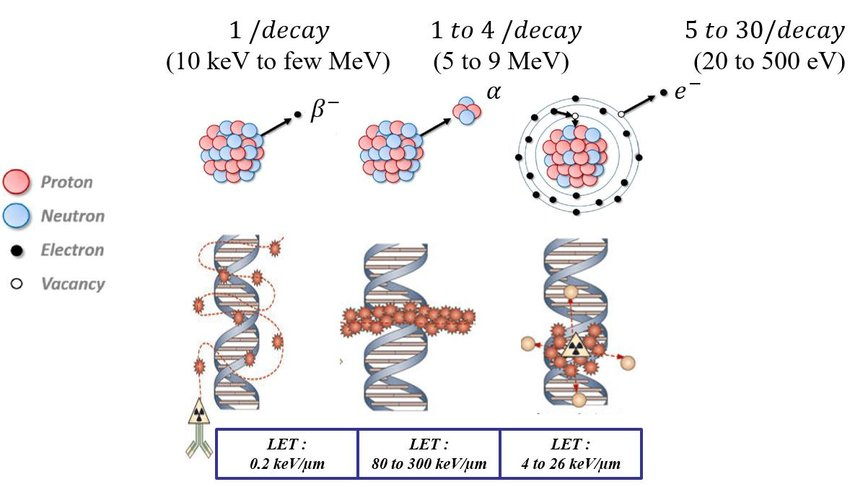
\includegraphics[scale=1]{Theory/DNA_LET.jpg} 
	\caption{Figure shows DNA .. \textcolor{red}{Cannot find citation anymore?} }
	\label{fig:DNA_damage}
\end{figure}



External beam therapy utilizes the stoppingpower \textcolor{blue}{(is stoppingpower for photons as well?)} of particles like photons (X-rays), electrons and hadrons \textcolor{red}{find a citation}, so that most of the energy is deposited at the site of the tumor. Particles interact differently dependent on their mass and charge. Figure \ref{fig:particles_Edeposition} shows an overview of how different particles deposit energy in a medium. Photons has a long build-up where the secondary electrons increas the dose up to a certain depth. The depth of the maximum dose is dependent on the energy, and thus by varying the energy, the tumor can be exposed to most of the radiation. 


\begin{figure}
	\centering
	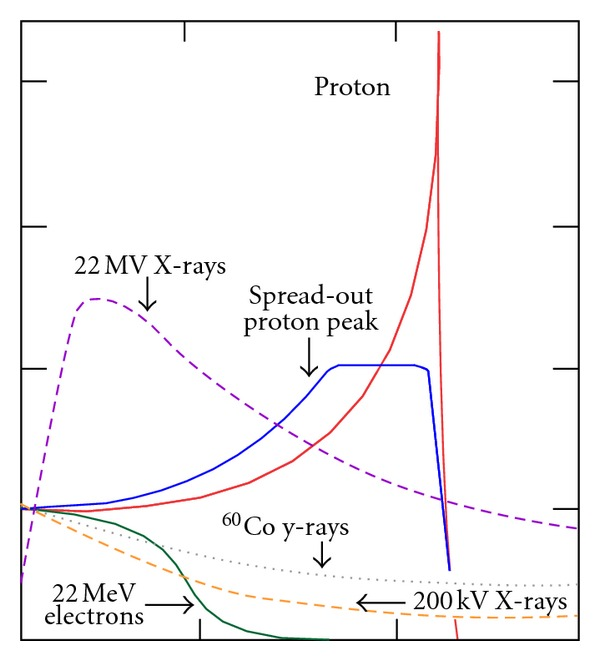
\includegraphics[scale=1]{Theory/Bragg-peak-and-Spread-Out-Bragg-Peak-SOBP-for-a-proton-beam-in-comparison-with-photon.jpg}  
	\caption{Particles energy deposition in a medium. Lacks axis. \textcolor{red}{find citation in special curriculum} }
	\label{fig:particles_Edeposition}
\end{figure}









here write about external beam therapy and targeted radionuclide therapy. 
Write about the LET curve. LET stoppingpower. 




\chapter{The use of medical isotopes in imaging and therapy}\label{Chapter:Medical_Isotopes}
\noindent


\section{History + Where we are today}

\subsection{External and internal radiotherapy }
General about external, internal, how they differ. Write most about internal, and the use of tracers, the different possibilities. 


Today, several treatments are used to cure cancer, among the most commonly used methods; chemotherapy, surgery, external beam therapy and immunotherapy.  External beam therapy utilizes the stopping power of particles like photons (X-rays), electrons, protons and heavier ions, to deposit most of the energy at the site of the tumor. Depending on the tissue, depth and shape of tumor and the energy of the particles, a dose plan can be made which will maximize the effect over the tumor and spare as much as the healthy tissue as possible. However, it has its limitations. Firstly it can only give dose to one single tumor, so the the specific use of external beam is not enough if the cancer has spread. The exposure of healthy tissue will be present, although methods using heavy ions can give a more specific dose, due to the Bragg-peak from Bethe-Block. \newline

\noindent
The idea behind targeted radionuclide therapy is to use radiopharmaceuticals which consist of a radionuclides which emit short-range ionizing particles, and a cell-targeting vector which can target specific cancer cells. Figure \ref{fig:interna_external} shows an illustration of how internal and external therapy differs. Using this type of treatment, it is possible to give a more localized dose, and even treat metastasis. But it does require knowledge of the biology, and how the biological update and half life is. Characteristics which are typical for all radionuclides used in therapy is that it should have sufficient long half life, so that it can be targeted in cancer cells but washed out of the body before too much dose is deposited. For imaging  where you would like to have short half life, so that the patient will not remain radioactive after the imaging. The size of the radiopharmaceutical should not be too large, especially if brain is targeted, because of the blood brain barrier. 

A limitation of targeted radionuclide therapy is that we can not see where the dose is actually deposited. This is why looking for theranostic pairs; one radionuclide which emit gammas or positrons for imaging (PET or SPECT) and one radionuclide used for treatment, emitting short range particles. The pair should have similar physical and chemical properties so they are taken up in equal quanta in the body, the imaging agent should have a short half life and treatment agent should have a longer half life. \textcolor{red}{look up what the actual half lives should be.} 

\begin{figure}
    \centering
    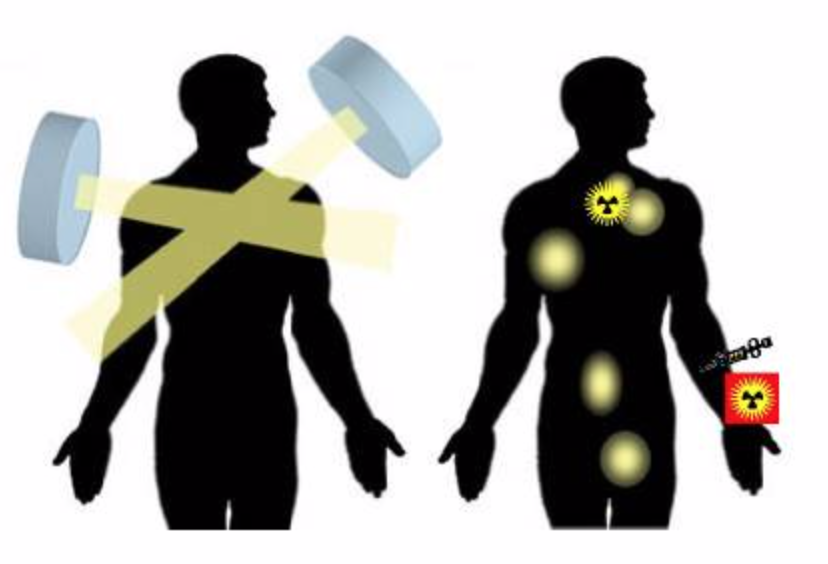
\includegraphics[width=0.5\textwidth]{Theory/internal_vs_external.png}
    \caption{Figure shows how external beam therapy works in comparison to targeted radionuclide therapy. Picture is accessed from \cite{figure_internal_external}}
    \label{fig:interna_external}
\end{figure}


\section{Medical isotopes}

\subsection{General characteristics}
Biological and physical properties. 
LET
Decay types 





\section{Platinum isotopes used in medicine} 

\subsection{Pt-193m}
potential, decay, how it is thought to be used. 

\section{History + Where we are today}

\subsection{External and internal radiotherapy }
General about external, internal, how they differ. Write most about internal, and the use of tracers, the different possibilities. 


Today, several treatments are used to cure cancer, among the most commonly used methods; chemotherapy, surgery, external beam therapy and immunotherapy.  External beam therapy utilizes the stopping power of particles like photons (X-rays), electrons, protons and heavier ions, to deposit most of the energy at the site of the tumor. Depending on the tissue, depth and shape of tumor and the energy of the particles, a dose plan can be made which will maximize the effect over the tumor and spare as much as the healthy tissue as possible. However, it has its limitations. Firstly it can only give dose to one single tumor, so the the specific use of external beam is not enough if the cancer has spread. The exposure of healthy tissue will be present, although methods using heavy ions can give a more specific dose, due to the Bragg-peak from Bethe-Block. \newline

\noindent
The idea behind targeted radionuclide therapy is to use radiopharmaceuticals which consist of a radionuclides which emit short-range ionizing particles, and a cell-targeting vector which can target specific cancer cells. Figure \ref{fig:interna_external} shows an illustration of how internal and external therapy differs. Using this type of treatment, it is possible to give a more localized dose, and even treat metastasis. But it does require knowledge of the biology, and how the biological update and half life is. Characteristics which are typical for all radionuclides used in therapy is that it should have sufficient long half life, so that it can be targeted in cancer cells but washed out of the body before too much dose is deposited. For imaging  where you would like to have short half life, so that the patient will not remain radioactive after the imaging. The size of the radiopharmaceutical should not be too large, especially if brain is targeted, because of the blood brain barrier. 

A limitation of targeted radionuclide therapy is that we can not see where the dose is actually deposited. This is why looking for theranostic pairs; one radionuclide which emit gammas or positrons for imaging (PET or SPECT) and one radionuclide used for treatment, emitting short range particles. The pair should have similar physical and chemical properties so they are taken up in equal quanta in the body, the imaging agent should have a short half life and treatment agent should have a longer half life. \textcolor{red}{look up what the actual half lives should be.} 

\begin{figure}
    \centering
    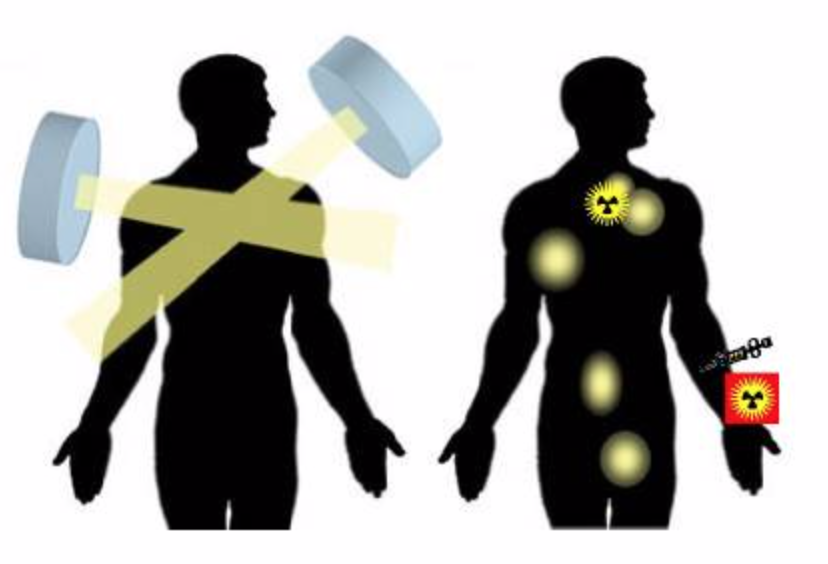
\includegraphics[width=0.5\textwidth]{Theory/internal_vs_external.png}
    \caption{Figure shows how external beam therapy works in comparison to targeted radionuclide therapy. Picture is accessed from \cite{figure_internal_external}}
    \label{fig:interna_external}
\end{figure}


\section{Medical isotopes}

\subsection{General characteristics}
Biological and physical properties. 
LET
Decay types 





\section{Platinum isotopes used in medicine} 

\subsection{Pt-193m}
potential, decay, how it is thought to be used. 

\section{General nuclear reaction theory}

\subsection{Nuclear reactions and reaction cross sections}

A nuclear reaction in the energy ranges of isotope production via the Compound nucleus conserves quantities such as mass-energy, linear momentum, the total number of nucleons, angular momentum and parity. A nuclear reaction is denoted as
\begin{equation}
    X(a,b)Y
\end{equation}


\noindent where X is the target, a is the incoming projectile, b is the outgoing decay channel and Y is the product of the nuclear reaction (Krane, chapter 11.1). There are multiple processes which can occur, radiative capture is the process where a particle is captured and a $\gamma$-ray is emitted in a (x,$\gamma$) process. If the incoming and outgoing particle is the same, it is a scattering process, where elastic scattering leaves the target nucleus in the energy same state, and inelastic if the target nucleus is in an excited state. In these type of experiments however, we are interested in emission of particles to create products in which we can measure the reaction cross section. \\

\noindent 
The cross section for a reaction can be divided into the cross section of the formation of the compound nucleus via interaction with the incoming projectile a, and the probability that the compound nucleus decay by decay channel b. The total reaction cross section is thus the sum of all the different reaction channels, 
\begin{equation}
    \sigma = \sum_b \sigma(a,b)
\end{equation}
where b can be multiple particles. The general equation which is used to calculate cross sections in this experiment is the following equation

\begin{equation}
    \sigma(E) = \frac{A_0 \cdot t_\text{irr}}{N_T \cdot \Phi(E)(1-e^{-\lambda t_\text{irr}})}
\end{equation}
\noindent where $A_0$ is the end of beam activity of the resulting product nucleus (Y), $t_\text{irr}$ is the irradiation time, $N_T$ is the number of target nuclei (X), $\Phi(E)$ is the projectile flux (a), and $\lambda$ is the decay constant of the product nucleus. \\ 

\noindent The compound nucleus model (Bohr, 1936) is a model which describes the formation of a compound nucleus by absorption of an incoming projectile by a nucleus close enough to interact with the strong nuclear force, and the decay of the compound nucleus. The kinetic energy shared between the incoming projectile and the nucleon which was struck leads to multiple collisions with other nucleons and rapid exchange of energy. The energy is distributed throughout the nucleus, leaving the original nucleus in an highly excited state. The average energy per nucleon is not sufficient to overcome the binding energy of the nucleus, but due to the statistical distribution in energies there is a probability that one or more nucleons may get sufficient energy to escape the nuclear potential (Krane, chapter 11.10, p. 416). This is decay of the compound nucleus, and this will lower the excitation energy. We can include the formation of the compound nucleus in the nuclear reaction as \begin{equation}
    X + a \rightarrow C^* \rightarrow Y + b
\end{equation} where $C^*$ is the excited compound nucleus (Krane, chapter 11.10, p. 416)  \\

\noindent For each possible decay channel of the compound nucleus, there is an associated probability or cross section, which is dependent on the energy of the incoming projectile. A function which evaluates the various cross sections at different energies is called an excitation function. In figure \ref{fig:pt_reactionchannels}, the excitation function of the reactions channels for the platinum isotopes $^{188, 189, 191,193m}$Pt resulting from deutrons on natural iridium is plotted. The nuclear chart for these reaction channels can be seen in figure \ref{fig:chart_irpt}. Natural iridium consists of two stable isotopes, $^{191}$Ir (37.3\% abundance) and $^{193}$Ir (62.7\% abundance). $^{193m}$Pt can only be produced from $^{193}$Ir, ejecting 2 neutrons in the process, which can be denoted as $^{193}$Ir(d,2n)$^{193m}$Pt ($^{193}$Pt is the compound nucleus formation of deutron on $^{191}$Ir, which has a low production cross section). The other platinum isotopes can be produced as $^{191}$Ir(d,2n)$^{191}$Pt or $^{193}$Ir(d,4n)$^{191}$Pt, $^{191}$Ir(d,4n)$^{189}$Pt or $^{193}$Ir(d,6n)$^{189}$Pt and $^{191}$Ir(d,5n)$^{188}$Pt or $^{193}$Ir(d,7n)$^{188}$Pt. For each reaction route possible, there is a local maxima for the specific route \textcolor{red}{what is the edges on 188, 189 and 191Pt?}. Hence, $^{193m}$Pt has only one maxima, and the other platinum isotopes has two. The desired particle emission is energy dependent, and the higher energy given to the compound nucleus, the probability that more particles will be emitted is higher (Krane, chapter 11.10, p. 419). When a specific isotope is desired, the excitation function can tell us which energy window that maximizes the production and most importantly minimizes particularly other isotopes of the same element, due to the difficulty of separating same chemical elements. \\


\begin{figure}
    \centering
    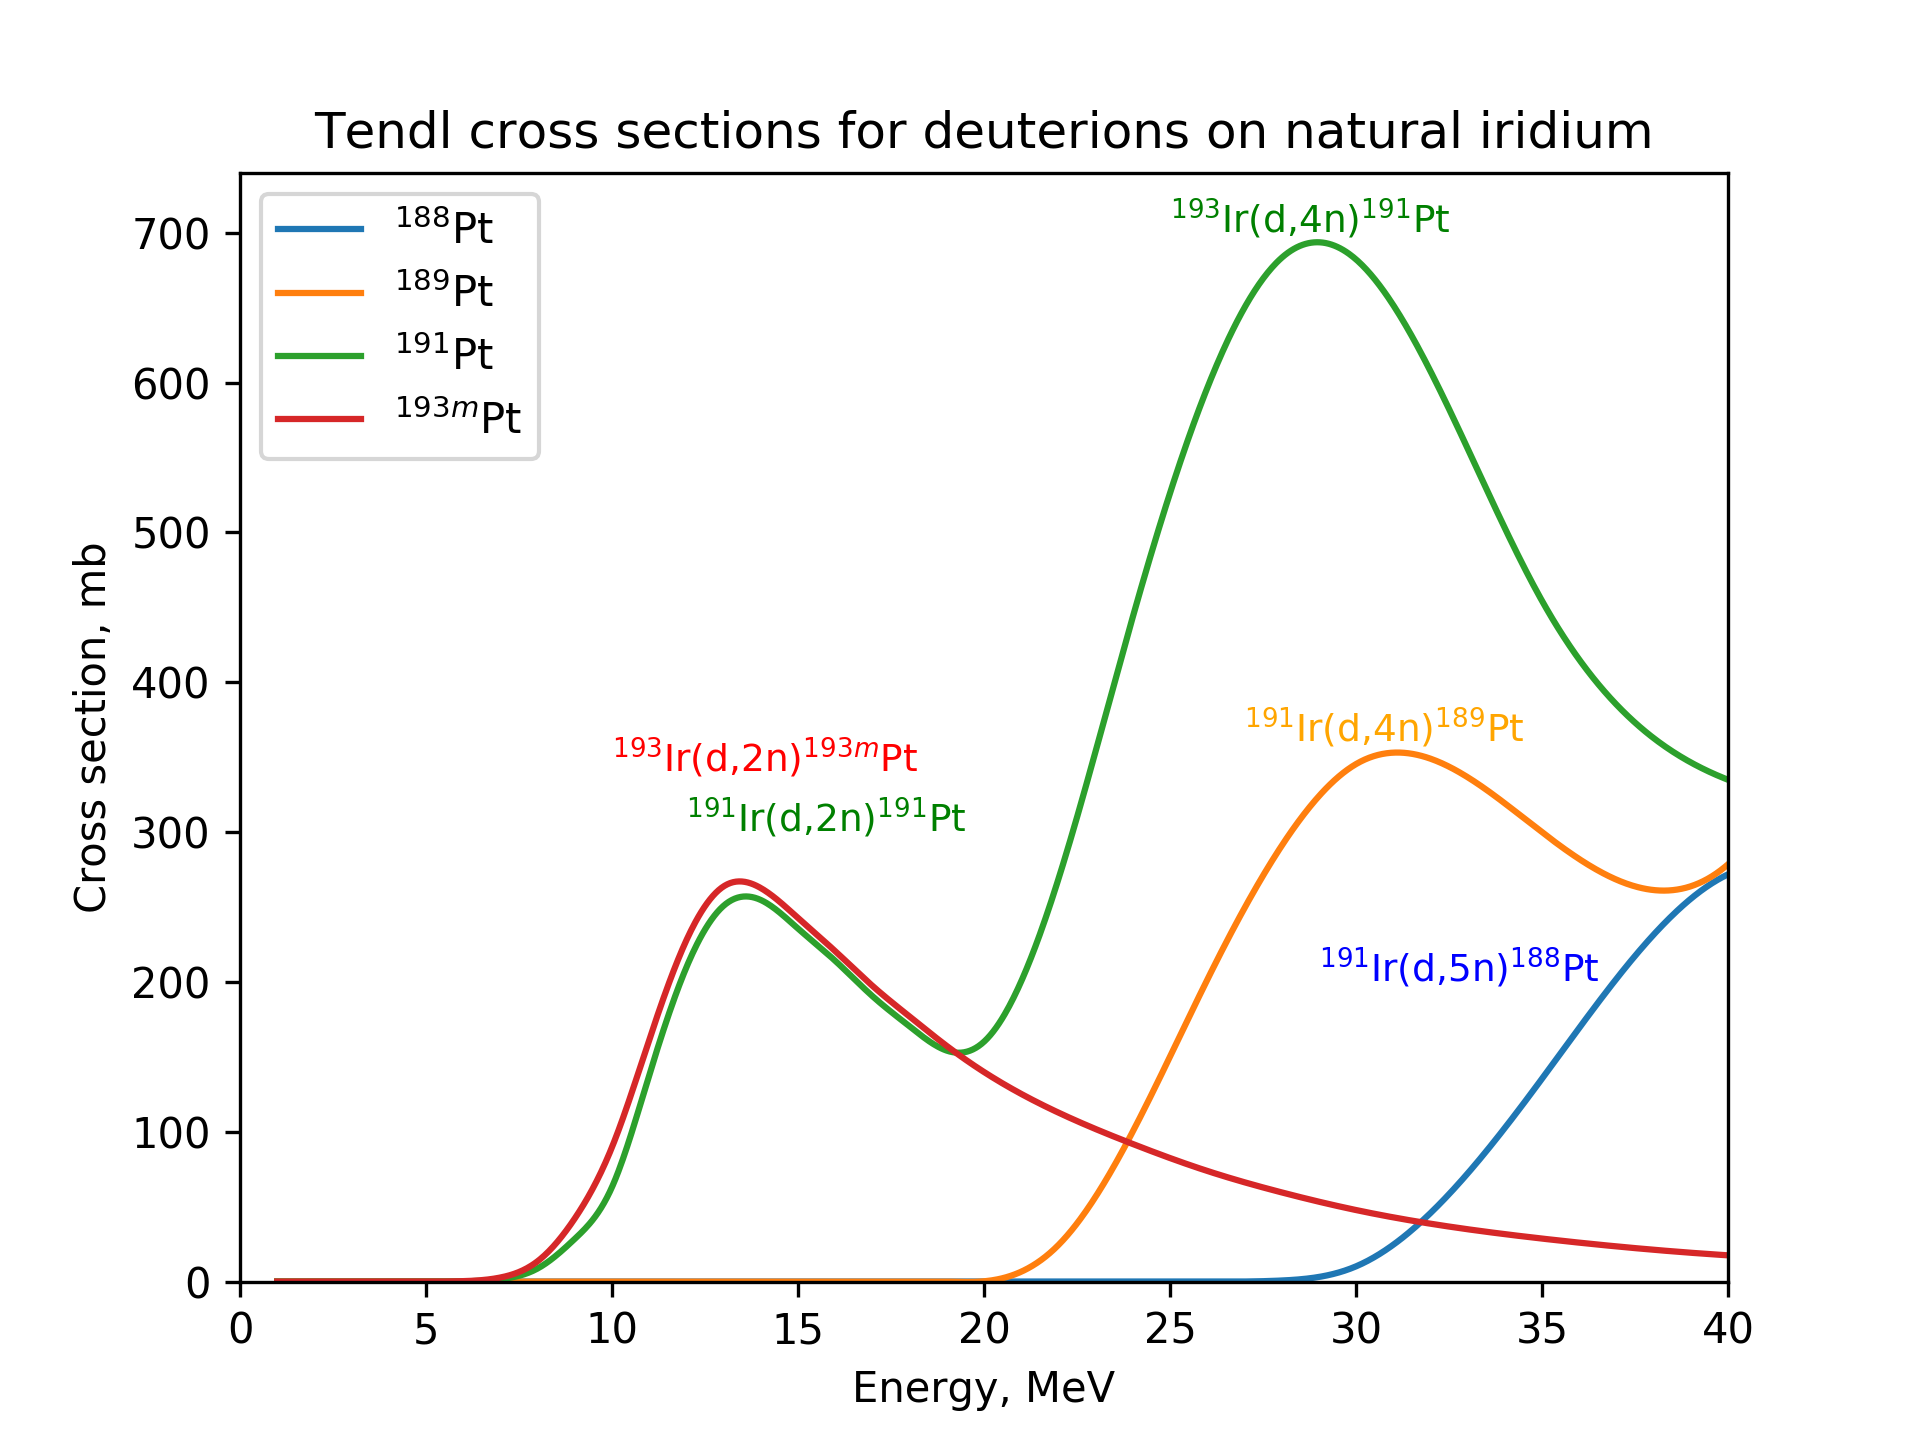
\includegraphics{Theory/reactionchannels_pt.png}
    \caption{Reaction cross sections provided by Tendl for the reactions $^\text{nat}$Ir(d,x)$^{188,189,191,193m}$Pt}
    \label{fig:pt_reactionchannels}
\end{figure}

\begin{figure}
    \centering
    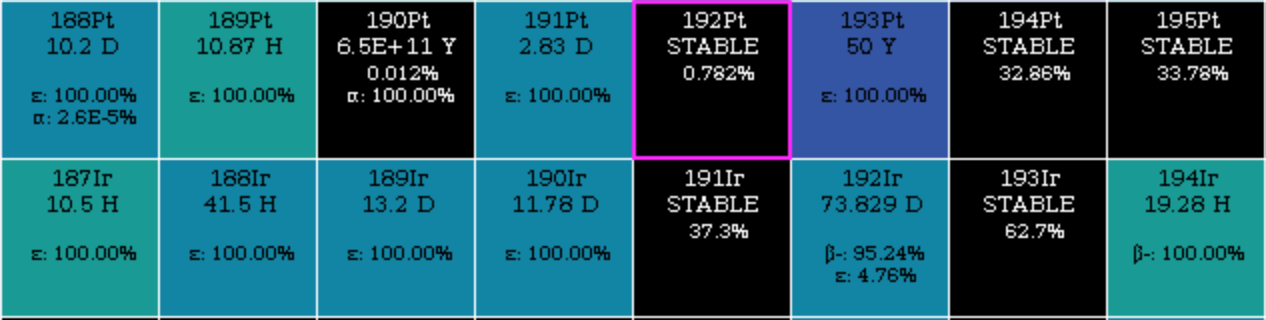
\includegraphics[width=12cm]{Theory/Ir(d)Pt.png}
    \caption{Nuclear chart for the platinum isotopes which can be produced from natural iridium }
    \label{fig:chart_irpt}
\end{figure}



%\noindent A nuclear reaction
%The nucleus is built up on protons and neutrons, and these are bound through the strong nuclear force. 
\subsection{Energetic factors in nuclear reactions}



%\noindent The binding energy depends on multiple parameters, which are based upon two models, the shell model and the liquid drop model (Krane, chapter 3.3, p. 68). The binding energy thus depends on the volume, which is constant throughout the nucleus, hence a volumeterm $a_V\cdot A$, a the surface of the nucleus which needs to be taken into account, since the nucleons on the surface is less tightly bound, $a_s\cdot A^{2/3}$. 
The nucleus is bound together by the strong nuclear force in the nuclear potential well, with a radius up to a few femtometer. The nuclear potential can be illustrated in figure \ref{fig:sumOfPotentials}, denoted as \textit{nuclear potential}. The Coulomb barrier is a repulsive barrier for charged particles. For a charged particle induced nuclear reaction, the energy should exceed to potential, or there will be an elastic scatter. However, there is a chance of tunneling, which drops with a factor 1/r where r is the distance from the center of the nucleus (Handbook of Nuclear Chemistry, chapter 3 - Nuclear Reactions, section, 3.2.3). The barrier also constraints the emission of particles for a decay channel of the compound nucleus, as the energy for an outgoing decay channel of positive particles must exceed the barrier. There is also a centrifugal barrier, which is dependent on the orbital angular momentum of the the nucleus. The orbital angular momentum is dependent on the mass and energy of the particle, but also the impact parameter of the reaction, which is the "distance" between the projectile and the nucleus

\begin{equation}
    \ell\hbar = (mv)b, \quad b\leq r_a + r_X
\end{equation}

\noindent where $r_a$ and $r_X$ are the radii of projectile and target nucleus. If $\ell=0$, the impact parameter is zero. If $\ell\neq 0$, then some of the energy of the projectile will go to rotational energy of the nucleus (Handbook of Nuclear Chemistry, chapter 3 - Nuclear Reactions, section, 3.2.4). The probability of this drops with $1/r^2$, and if the impact parameter is large, this will constraint some of the energy that would have gone to the nuclear reaction. Figure \ref{fig:sumOfPotentials} shows an overview of the various potentials; centrifugal barrier, Coulomb barrier and nuclear potential. The figure is for $^{58}$Zn, but the figure is only an example. \textcolor{red}{maybe make figure self?}. 


\begin{figure}
    \centering
    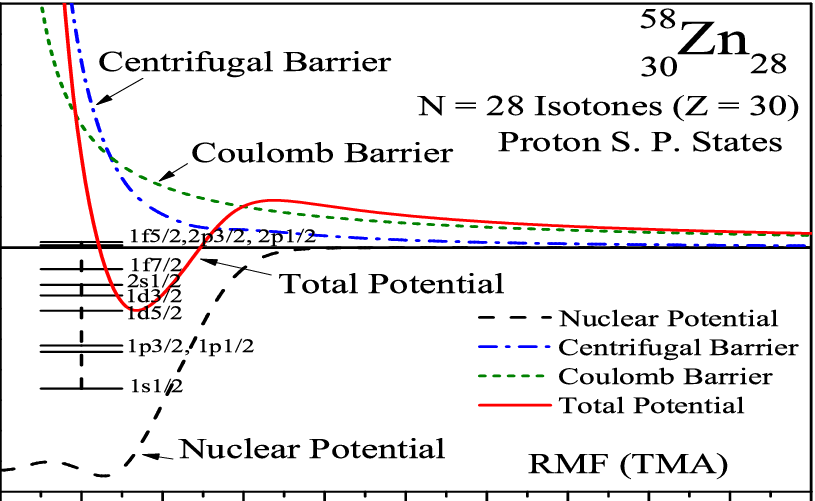
\includegraphics[width=8cm]{Theory/sum_of_potentials.png}
    \caption{The figure shows the nuclear potential well for the strong nuclear force, along with the Coulomb repulsion barrier and the centrifugal barrier for $^{58}$Zn. The figure is only meant as an illustration. %\url{https://www.researchgate.net/figure/The-RMF-potential-energy-sum-of-the-scalar-and-vector-potentials-for-the-nucleus-58-30_fig6_257811951} }
    }
    \label{fig:sumOfPotentials}
\end{figure}



\begin{comment}
\noindent The separation energy is the energy required to remove a particle from the nucleus. That is the difference in the binding energy for the two nuclei. The neutron separation energy is 
\begin{equation}
    S_n = B(^A_z X_n)-B(^{A-1}_z X_{n-1}) = c^2(m(X^{A-1}_zX_n)-()
\end{equation}\\ 
\end{comment}

\noindent In a nuclear reaction, the mass-energy is conserved, which is denoted as the Q-value. The reaction Q-value is the difference is masses between before and after the nuclear reaction occurred (Krane, chapter 11.2). It is defined as 

\begin{equation}
    Q = (m_i - m_f)c^2 = (m_X + m_a - m_Y - m_b)c^2
\end{equation}

\noindent where $m_i$ is the initial mass, $m_f$ is the final mass and c is the speed of light. If $Q>0$, then the reaction is exoergic, which means that energy is released in the reaction. There is no threshold energy of the projectile required for the reaction to occur, if only the projectile is present the reaction can occur. If $Q<0$, then the reaction is endoergic, which means that the kinetic energy of the incoming projectile is converted into nuclear mass or binding energy. For endoergic reactions to occur, there is a minimum threshold energy of the projectile in order for the reaction to happen, which is defined as (Krane, 11.2, p. 382)

\begin{equation} \label{eq:reaction_threshold}
    E_\text{threshold} = (-Q) \cdot \frac{m_Y +m_b}{m_Y + m_b -m_a}
\end{equation}


\noindent The energy threshold thus depend on the Q-value, the Coulomb barrier for charged particles, and the centrifugal barrier if angular momentum $\ell\neq 0$. The parity though depend, even numbers of $\ell$ mix with even, and odd with odd (Handbook of Nuclear Chemistry, chapter 3Nuclear Reactions, section, 3.2.3). This gives an indication on when a reaction can energetically occur, but does not tell us how probable the reaction is. Equation \ref{eq:reaction_threshold} indicates that a higher mass for the particle in the outgoing channel $m_b$, will lower the energy threshold.\\ 

The nuclear binding energy is a number which tells us how tightly bound the nucleus is, and much energy is required to separate nucleons from the nucleus. The nuclear binding energy is related to the mass of the nucleus, through the famous equation 
\begin{equation}
    E = mc^2
\end{equation}

\noindent 
The binding energy is the mass-difference between the nucleus as a whole, and the number of protons and neutrons added
\begin{equation} \label{eq:Binding_energy1}
    B = c^2(z\cdot m_p + n \cdot m_n - m_N)
\end{equation}
\noindent where z is the number of protons, n is the number of neutrons, $m_p$ is the proton mass, $m_n$ is the neutron mass, $M_N$ is the mass of of the nuclide, which is the number of nucleons A minus the number of electrons, $M_P = m_A - z\cdot m_e$ (the electronic binding energy per electron is excluded). From Krane's derivation of the nuclear binding energy (Krane, chapter 3.3, p. 65), the equal number of protons and neutrons make up $z\cdot^1H$, thus we can rewrite equation \ref{eq:Binding_energy1} to 

\begin{equation}
    B = z\cdot m_{^{1}H} + n\cdot m_n - m_{A}
\end{equation}

\noindent 
Separation energy of a particle is the energy required to be removed from the nucleus. This is defined as the difference in binding energy between the nucleus with the particle and the nucleus without the emitted particle. Since heaavier particles such as tritrium has a lower binding energy, more energetically easy to separate. n and p require more. 

\textcolor{red}{Write about the semi-empirical mass formula, and what terms that affects the decay of compound. Especially the parity term? Odd A or even A. If A odd, decay by proton, since then A is even. If A is even, then decay by alpha for A to remain even. But why is n,p favoured over for instance t?? }

\subsection{Nuclear cross sections}

The cross section for a reaction can be divided into the cross section of the formation of the compound nucleus via interaction with the incoming projectile a, and the probability that the compound nucleus decay by decay channel b. The total reaction cross section is thus the sum of all the different reaction channels, 
\begin{equation}
    \sigma = \sum_b \sigma(a,b)
\end{equation}
where b can be multiple particles. The general equation which is used to calculate cross sections in this experiment is the following equation

\begin{equation}
    \sigma(E) = \frac{A_0 \cdot t_\text{irr}}{N_T \cdot \Phi(E)(1-e^{-\lambda t_\text{irr}})}
\end{equation}
\noindent where $A_0$ is the end of beam activity of the resulting product nucleus (Y), $t_\text{irr}$ is the irradiation time, $N_T$ is the number of target nuclei (X), $\Phi(E)$ is the projectile flux (a), and $\lambda$ is the decay constant of the product nucleus. 

\newpage

Why we are interested, why is there a need for nuclear production cross sections. 



The Q-value for nuclear reactions 

Compound nucleus, what happens. 
Q value, binding energy, particle emission, probabilities (why does n, p/alpha emission require higher energy, but is more favoured than T emission if both possible.)


\subsection{Expected products from deuterions on iridium, iron, cupper and nc}

Include figure of different nuclear charts, and write about Q values, and reaction channels, which makes it more probable that we observe it (eg. when neutron, proton/alpha channels opens).





\chapter{Experimental setup} \label{Experiment}




\section{Lawrence Berkeley National Laboratory's 88" Cyclotron} \label{sec:Cyclotron}
\noindent

\textcolor{red}{Writing about the facility, and what is done there. Major accomplishments. Then about the type of experiment, stacked-target. They have done this before. Cyclotron facilities. }

Lawrence Berkeley National Laboratory (LBNL) is a national research laboratory on behalf of the Us. Department of Energy, and is operated by University of California, Berkeley. The laboratory starter up in 1928 by founder Ernest O. Lawrence, who is also the inventor of the cyclotron. \textcolor{red}{What other fields are researched upon in LBNL.} \textit{from wiki: Several great discoveries were done at LBNL, among some, oberservation of the antiproton, discovery of accelerating universe and transuranic elements. }

\noindent
The Lawrence Berkeley's 88" Cyclotron has many purposes, eg. isotope production for medical applications and heavy element search, and commercial use.  \textcolor{red}{Correct?} \\

\noindent
The  facility is figured in \ref{fig:LBNL_88}, and consist of a cyclotron vault, and experimental caves in which the beam can be bent to with bending magnets. Faraday cups can measure the beam current at different steps along the way, which makes it possible to measure the transition efficiency of the beam. Faraday cups are dense metal block, usually 6-7 cm broad Cupper and tantilum. It works as a beam stopper, and can be lowered into the beam line to measure the current. It is electrically isolated, which makes it possible to measure the current, since we know the number of initial particles accelerated. Due to electrons close to surface might be scattered of, can read of higher positive charge than what is correct. Put magnet around the cup to bend the electrons back to the Faraday cup in what is called magnetic suppression.
\noindent
Cave 0 is used mainly for neutron beam, chemistry, and isotope production, and was used for irradiation of the target stack. 

\begin{figure}
    \centering
    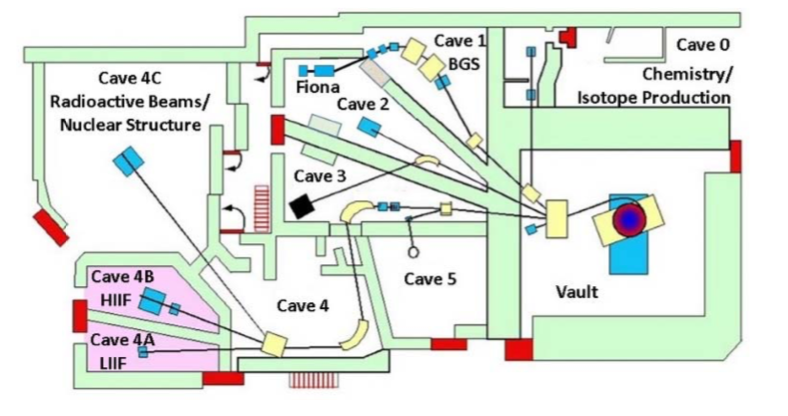
\includegraphics[width=0.5\textwidth]{Experiment/LBL_88.png}
    \caption{An overview of the facility.  Picture is from \cite{KireeffCovo2018}}
    \label{fig:LBNL_88}
\end{figure}

\subsection{General functionality of a Cyclotron}
Cyclotrons consist of two D-shaped electrodes shaped as a circle with a gap between, and an electromagnet consisting of two coils in which the electrode is placed between. This creates a magnetic field perpendicular to the electrodes. 
From the Lorentz Force, with a magnetic field perpendicular to an electric field will give a circular movement of a particle of charge $q$,

\begin{equation} \label{eq:Lorentz}
    \textbf{F} = q\textbf{E} + q\textbf{v} \times \textbf{B}
\end{equation}

An oscillating electric field is applied between the electrodes, which makes the particles accelerate over the gap between the electrode, be bent in a circular motion and accelerated back with the shifting electrical field. The frequency of the field is called the radio-frequency (RF), or the cyclotron resonance
\begin{equation}
    f = \frac{qB}{2\pi m}
\end{equation}
Particles which are not synchronized with the RF-field is lost \cite{KireeffCovo2018}. \textcolor{red}{Include figure of cyclotron?}  

We can rewrite equation \label{eq:Lorentz}, using the centripetal force, $F_c = \frac{mv^2}{r}$. Since the centripetal force works in the same direction as the magnetic field, we can set $F_c=qvB$, which gives the radius of the particle path 
\begin{equation}
    r = \frac{mv}{qB}
\end{equation}
With increasing velocity, the radius of the path increases. But to obtain the RF, the velocity of the particle must also increase, hence the acceleration over the gap. This way, particles moves in an outward spiral, until they have gained sufficient energy wanted. The cyclotron must be operated in a vacuum, so the beam is not attenuated due to air particles. 


%Description: Describe cross section equation and the different stuff that goes into the equation. Then why we care about the mass density, efficiency. 


\section{The experiment}



The experimental cross section for a nucleus is described in the following equation

\begin{equation} \label{eq:CrossSection_general}
    \sigma(\langle E \rangle) = \frac{A_0}{\rho\Delta r I (1-e^{-\lambda \Delta t})}
\end{equation}



where $\langle E \rangle$ is the average energy across the foil, $A_0$ (Bq) is the activity after end of beam, $\rho \Delta r$ is the areal density of the target (nuclei/cm$^2$), I is the beam current (A), $\lambda$ is the decay constant ($s^{-1}$) of the nucleus and $\Delta t$ (s) is the length of the irradiation. %$A_0$ is found through by backpropagation of activities measured at multiple timepoints after end of beam, and will be further described in section \textcolor{red}{end of beam activity section}. The mass density of an 

Description: Describe cross section equation and the different stuff that goes into the equation. Then why we care about the mass density, efficiency. 



\subsection{Target design}
\textit{\textcolor{red}{Also, write about thin targets, underfilled beam, advantageous.}}\\

\noindent 
In this experiment, a stack of ten thin $^{\text{nat}}$Ir (99.9\%), ten $^{\text{nat}}$Ni, ten $^{\text{nat}}$Cu and three $^{\text{nat}}$Fe foils were irradiated with 33 MeV deuterions to induce nuclear reactions  \textcolor{red}{(provide info about foils, like where they were bought, and abundance and purity of the metal)}. The design of the target stack is well described in the literature (Voyles2018). Using a stacked target in a cross section experiment provides cross sections at multiple energies due to the energy degradation of the beam in the stack. With each foil being approximately 25 $\mu$m in thickness, cross sections were measured within high precision on the energy. Deuterions on Nickel, Cupper and Iron have several well known cross sections, which was used to determine the beam current throughout the stack, by solving equation \ref{eq:CrossSection_general} for beam current, and using these cross sections. These reactions are called monitor reactions, and we were particularly interested in $^{\text{nat}}$Ni(d,x)$^{56,58}$Co, $^{\text{nat}}$Cu(d,x)$^{62, 63, 75}$Zn and $^{\text{nat}}$Fe(d,x)$^{56}$Co.  \\ 

%The targets are larger than the beam, hence underfilled. Then the correct nuc/cmˆ2 
\noindent
In this experiment, the beam was underfilled, meaning that the area of the target was larger than the beamspot. Hence the areal density was then used to calculate the quantity of how many nuclei per cm$^2$. Areal density is given as 
\begin{equation}
    \rho \Delta r = \frac{m}{A}
\end{equation}
\noindent
where m is the mass and A is the area. The uncertainty in each parameter was calculated using the standard deviation
\begin{equation}
    \sigma = \sqrt{\frac{1}{N}\sum_{i=1}^N (x_i - \overline{x})^2}
\end{equation}
\noindent
where N is the number of measurements, $x_i$ is a measurement and $\overline{x}$ is the average over all measurements. 

\noindent
The uncertainty in each parameter was estimated using the approximation for standard deviation for independent parameters, derived in equation \ref{eq:uncertainty_simplification}

\begin{equation}
    \Big(\frac{\delta \rho \Delta r}{\rho \Delta r}\Big)^2= \Big(\frac{\delta m}{m}\Big)^2 \Big(\frac{\delta A}{A}\Big)^2
\end{equation}

\noindent 
The foils were cut into approximately 25 by 25 mm squares. Each foil was characterized using a caliper\footnote{MITUTOYO, ABSOLUTE DIGIMATIC} to measure the length of each side, a gauge caliper\footnote{MITUTOYO, IP65 COOLANT PROOF} to measure the thickness, and a weight\footnote{METTLER TOLEDO} was used to weight each foil which were pre-washed with isopropanol. For each foil, the length (across all sides) and thickness was measured at four different locations along the foils (they were not completely uniform). The foils were weighted four times as well. The thickness was not used in the calculation of the mass density, but was a good indication that the foil thicknesses were consistent. Conversion of the areal density to nuclei/$cm^2$ was done numerically, by multiplying by Avogadro's number and dividing by the mol-mass of the target.

\noindent
Table \ref{table:foil_characterization} shows the target stack with average values for length, thickness and areal density, and calculated areal density (in the order they were irradiated). After characterization, each foil was mounted on a plastic frame, and attached with capton tape along the edges. The target frames can be seen in figure \ref{fig:targetframe}. 


\begin{table}[h!]
%\centering
\caption{Characterization of each foil, along with calculated mass density. Each length is measured in mm, and mass in grams. }
\label{table:foil_characterization}
\small
\begin{tabular}{lllllll}
\makecell{\textbf{Foil}} & \makecell{Length1 (mm)}  &  \makecell{Length2 (mm)} & \makecell{Thickness (mm)} & \makecell{Mass (g)} & \makecell{\textbf{Mass density (mg/cm$^2$)}} \\ 
\hline
\makecell{SS1} & \makecell{} & \makecell{} & \makecell{} & \makecell{} & \makecell{\textbf{...}} \\
\hline
\makecell{Ni01} & \makecell{25.228} & \makecell{25.293} & \makecell{0.0285} & \makecell{0.1453} & \makecell{22.772 $\pm$ 0.138} \\
\makecell{Ir01} & \makecell{24.943} & \makecell{24.968} & \makecell{0.0295} & \makecell{0.3436} & \makecell{55.174 $\pm$ 0.053} \\
\makecell{Cu01} & \makecell{25.553} & \makecell{24.883} & \makecell{0.0341} & \makecell{0.1420} & \makecell{22.338 $\pm$ 0.048} \\
\makecell{Fe01} & \makecell{24.400} & \makecell{26.068} & \makecell{0.0278} & \makecell{0.1274} & \makecell{20.030 $\pm$ 0.110} \\
\hline
\makecell{Ni02} & \makecell{25.288} & \makecell{25.428} & \makecell{0.0295} & \makecell{0.1487} & \makecell{23.118 $\pm$ 0.096} \\
\makecell{Ir02} & \makecell{24.923} & \makecell{25.005} & \makecell{0.0278} & \makecell{0.3465} & \makecell{55.601 $\pm$ 0.238} \\
\makecell{Cu02} & \makecell{25.443} & \makecell{25.550} & \makecell{0.0348} & \makecell{0.1451} & \makecell{22.325 $\pm$ 0.028} \\
\makecell{Fe02} & \makecell{25.525} & \makecell{23.800} & \makecell{0.0274} & \makecell{0.1216} & \makecell{20.017 $\pm$ 0.034} \\
\hline
\makecell{Ni03} & \makecell{25.295} & \makecell{25.210} & \makecell{0.0270} & \makecell{0.1425} & \makecell{22.338 $\pm$ 0.066} \\
\makecell{Ir03} & \makecell{24.885} & \makecell{24.983} & \makecell{0.0243} & \makecell{0.3459} & \makecell{55.643 $\pm$ 0.121} \\
\makecell{Cu03} & \makecell{25.560} & \makecell{25.508} & \makecell{0.0343} & \makecell{0.1455} & \makecell{22.313 $\pm$ 0.043} \\
\makecell{Fe03} & \makecell{26.113} & \makecell{25.235} & \makecell{0.0310} & \makecell{0.1315} & \makecell{19.948 $\pm$ 0.114} \\
\hline
\makecell{Ni04} & \makecell{25.303} & \makecell{24.888} & \makecell{0.0273} & \makecell{0.1304} & \makecell{20.704 $\pm$ 0.068} \\
\makecell{Ir04} & \makecell{24.960} & \makecell{24.833} & \makecell{0.0261} & \makecell{0.3471} & \makecell{56.000 $\pm$ 0.109} \\
\makecell{Cu04} & \makecell{25.153} & \makecell{25.603} & \makecell{0.0333} & \makecell{0.1435} & \makecell{22.284 $\pm$ 0.027} \\
\hline
\makecell{Ni05} & \makecell{25.325} & \makecell{25.495} & \makecell{0.0263} & \makecell{0.1406} & \makecell{21.768 $\pm$ 0.045} \\
\makecell{Ir05} & \makecell{24.948} & \makecell{24.958} & \makecell{0.0256} & \makecell{0.3435} & \makecell{55.161 $\pm$ 0.081} \\
\makecell{Cu05} & \makecell{25.213} & \makecell{25.573} & \makecell{0.0334} & \makecell{0.1447} & \makecell{22.443 $\pm$ 0.028} \\
\hline
\makecell{Ni06} & \makecell{25.530} & \makecell{25.195} & \makecell{0.0285} & \makecell{0.1471} & \makecell{22.861 $\pm$ 0.123} \\
\makecell{Ir06} & \makecell{24.760} & \makecell{24.960} & 
\makecell{0.0240} & \makecell{0.3444} & \makecell{55.731 $\pm$ 0.088} \\
\makecell{Cu06} & \makecell{25.343} & \makecell{25.513} & \makecell{0.0340} & \makecell{0.1448} & \makecell{22.396 $\pm$ 0.012} \\
\hline
\makecell{Ni07} & \makecell{25.338} & \makecell{25.278} & \makecell{0.0268} & \makecell{0.1479} & \makecell{23.092 $\pm$ 0.078} \\
\makecell{Ir07} & \makecell{24.955} & \makecell{25.008} & \makecell{0.0278} & \makecell{0.3538} & \makecell{56.685 $\pm$ 0.085} \\
\makecell{Cu07} & \makecell{25.625} & \makecell{25.248} & \makecell{0.0326} & \makecell{0.1444} & \makecell{22.320 $\pm$ 0.014} \\
\hline
\makecell{Ni08} & \makecell{25.205} & \makecell{24.950} & \makecell{0.0256} & \makecell{0.1409} & \makecell{22.409 $\pm$ 0.124} \\
\makecell{Ir08} & \makecell{24.723} & \makecell{24.985} & \makecell{0.0281} & \makecell{0.3585} & \makecell{58.030 $\pm$ 0.130} \\
\makecell{Cu08} & \makecell{25.370} & \makecell{24.885} & \makecell{0.0333} & \makecell{0.1414} & \makecell{22.401 $\pm$ 0.033} \\
\hline
\makecell{Ni09} & \makecell{25.220} & \makecell{25.378} & \makecell{0.0257} & \makecell{0.1392} & \makecell{21.741 $\pm$ 0.073} \\
\makecell{Ir09} & \makecell{24.670} & \makecell{24.993} & \makecell{0.0273} & \makecell{0.3494} & \makecell{56.669 $\pm$ 0.043} \\
\makecell{Cu09} & \makecell{25.390} & \makecell{26.455} & \makecell{0.0331} & \makecell{0.1506} & \makecell{22.425 $\pm$ 0.041} \\
\hline
\makecell{Ni10} & \makecell{25.285} & \makecell{24.405} & \makecell{0.0271} & \makecell{0.1425} & \makecell{23.093 $\pm$ 0.024} \\
\makecell{Ir10} & \makecell{24.973} & \makecell{24.980} & \makecell{0.0270} & \makecell{0.3435} & \makecell{55.065 $\pm$ 0.055} \\
\makecell{Cu10} & \makecell{25.470} & \makecell{25.338} & \makecell{0.0355} & \makecell{0.1440} & \makecell{22.314 $\pm$ 0.047} \\
\hline


\hline
\makecell{SS2} & \makecell{} & \makecell{} & \makecell{} & \makecell{} & \makecell{\textbf{...}} \\
\makecell{P-degrader} & \makecell{} & \makecell{} & \makecell{} & \makecell{} & \makecell{\textbf{...}} \\
\makecell{Ni neutron monitor} & \makecell{} & \makecell{} & \makecell{} & \makecell{} & \makecell{\textbf{...}} \\
\hline
\end{tabular}
\end{table}

\begin{figure}
    \centering
    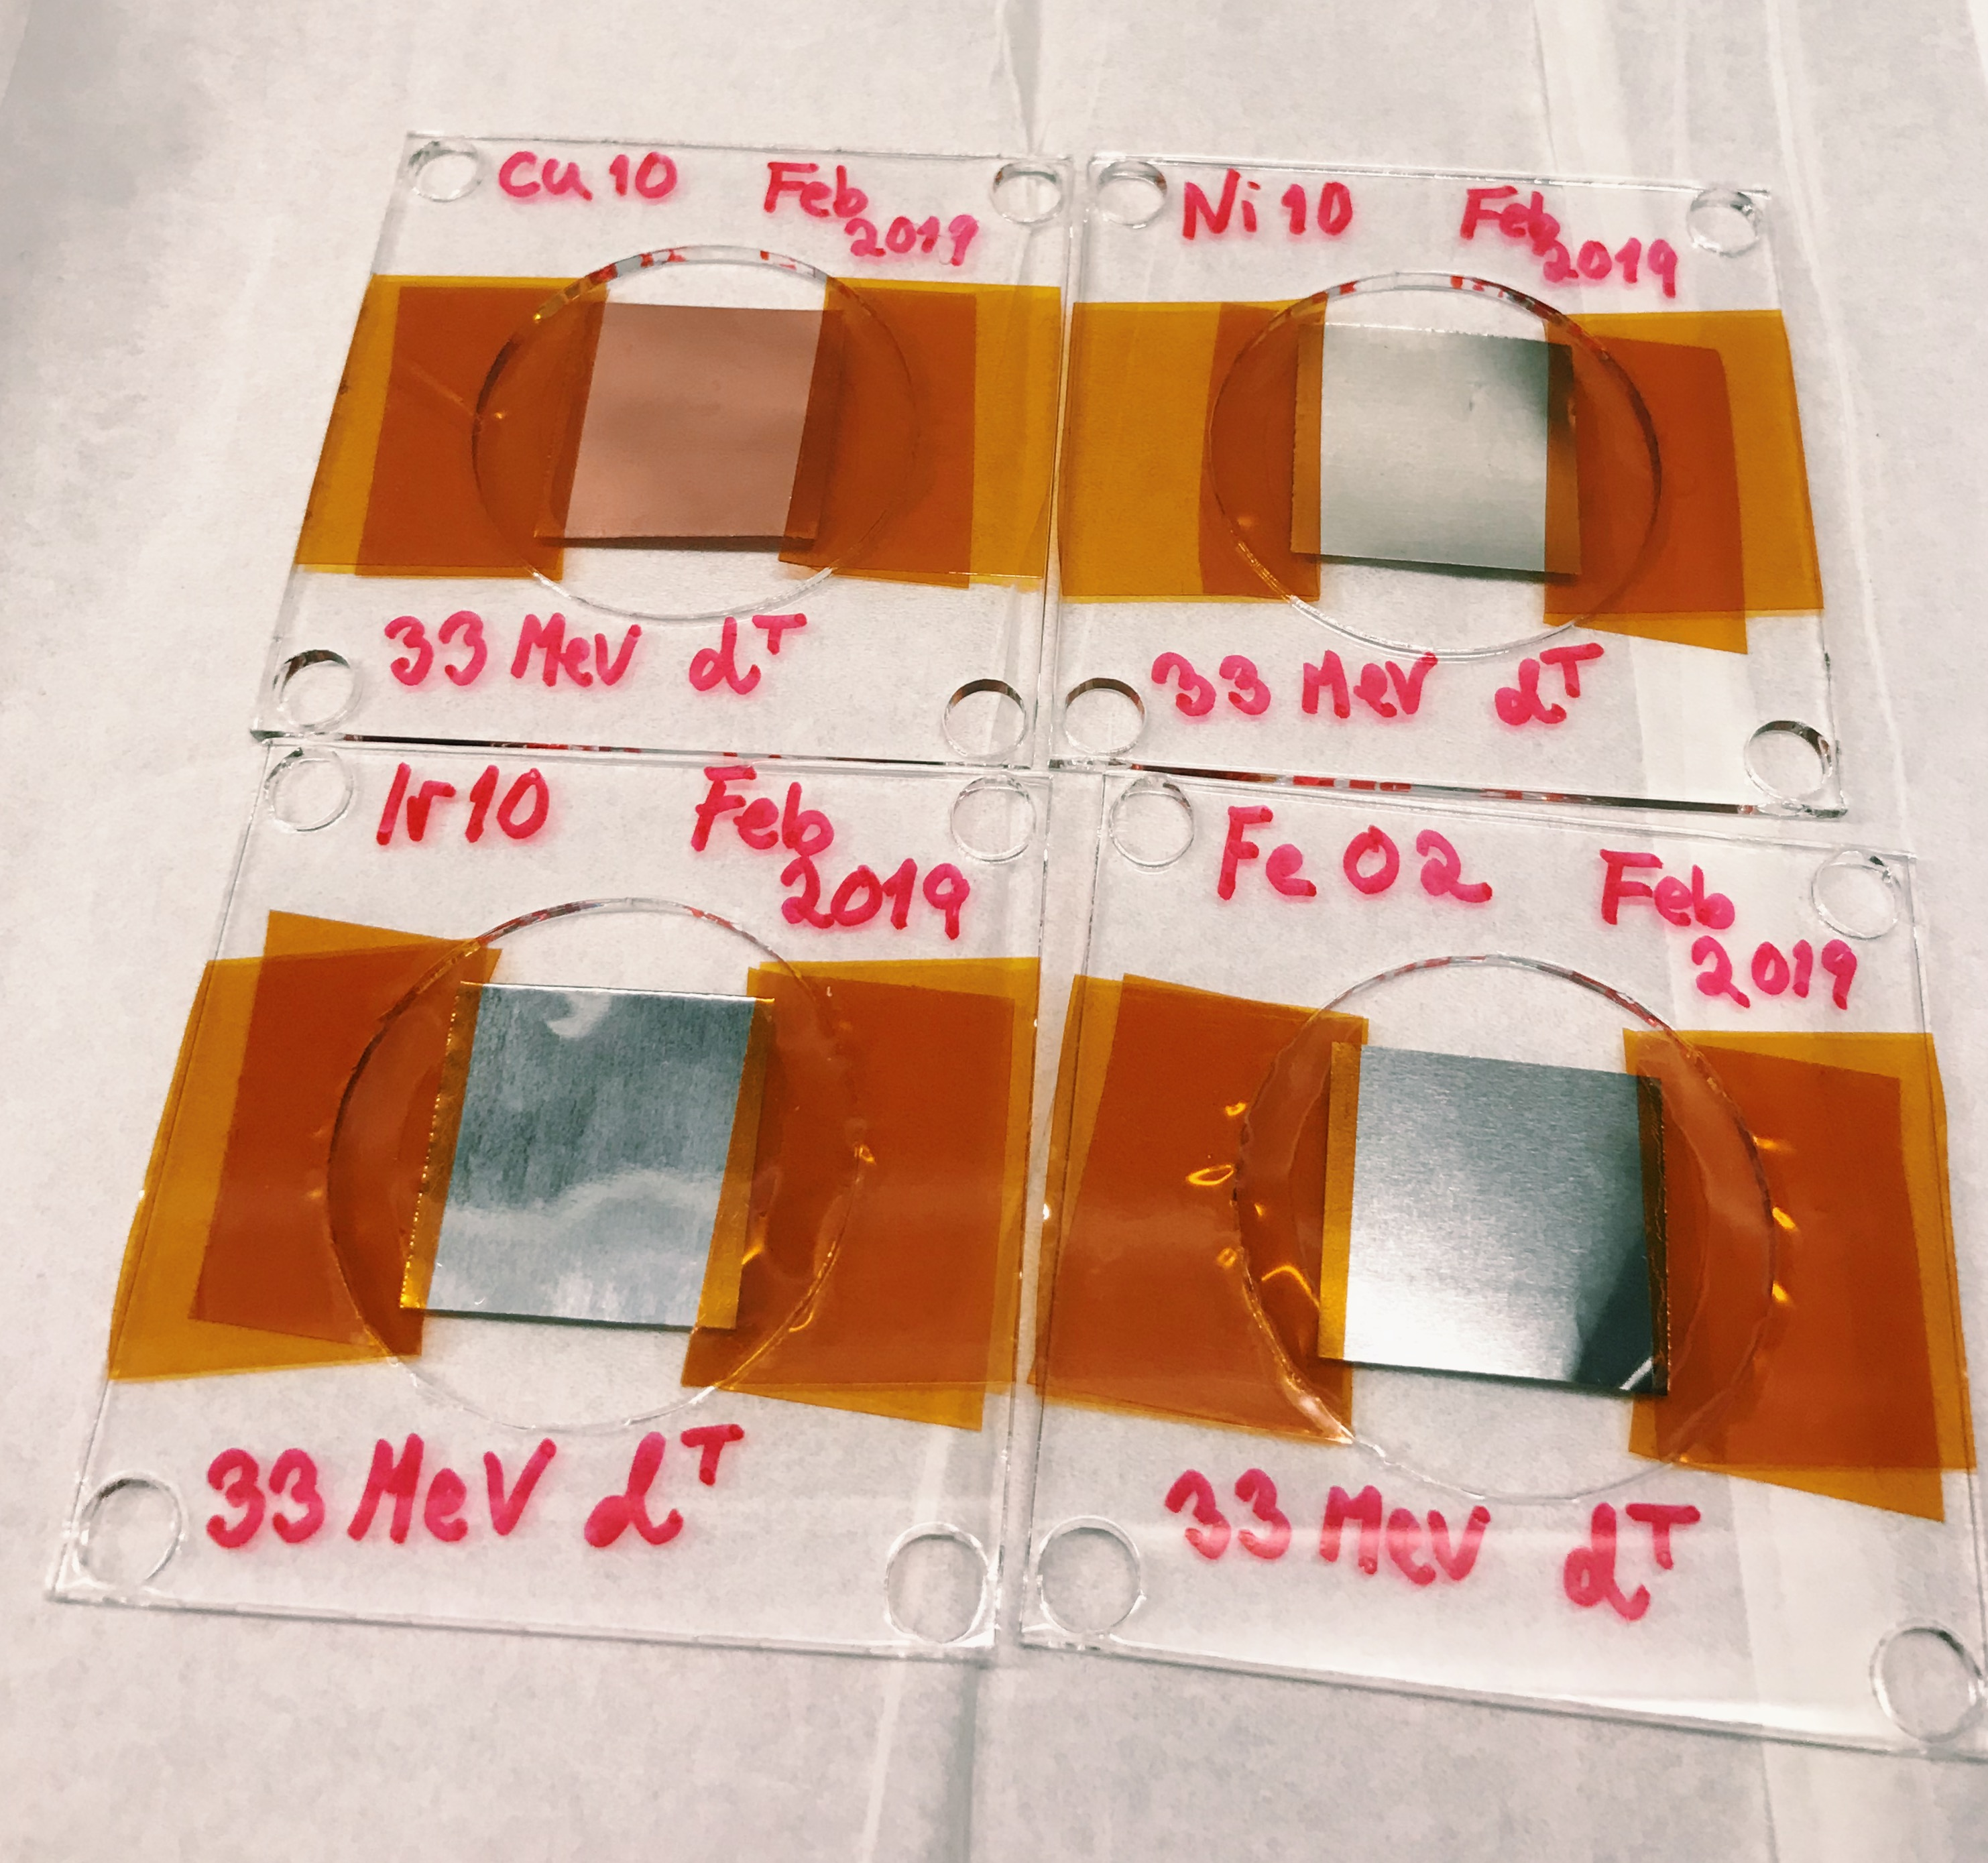
\includegraphics[width=8cm]{Experiment/targetframe.JPG}
    
    \caption{The target foils were mounted on plastic frames using capton tape. }
    \label{fig:targetframe}
\end{figure}

\subsection{Detector calibration}
In this experiment, seven different high purity Germanium detectors (HPGe) were used to measure the activity in each foil at multiple timepoints after end of beam. The HPGe-detector is a type of semiconductor, which is a material where the energy required to remove an electron from the valence band (in the outer atomic shell) to the conduction band is small. A Germanium atom has atomic number 32, and 4 valence electrons in the outer p4 shell. The atoms are bound through covalent bonds in a crystal structure. The main mechanism of a semiconductor detector is creation of electron-hole pairs after energy deposition of an ionizing particle in the crystal. If an electron is excited to the conduction band, a hole is left. The hole can move as a neighbooring electron fills this spot, and it can cause a chain reaction, and the hole will move in the crystal. Both the electron in the conduction band and the hole in  the valence band contributes to an electric current. Under influence of an electric field, the electron-hole pairs will be collected, and we can measure the incidence as a count. The major advantage with semiconductor detector is that the average energy to create an electron-hole pair is very low, which results in a superior energy resolution in comparison to other detectors like gas and scintillation detectors. \textcolor{red}{High energy resolution advantageous in gamma-ray spectroscopy which makes it possible to separate to gamma-ray peaks within less than a keV.} At room temperature,  thermal energy can excite the electron from the valence to the conduction band and cause noise in spectra. Therefor, Germanium detectors are operated at 0 Kelvin. \textcolor{red}{Write about recombination and trapping, noise, np semiconductor junction, depletion depth??}. (Techniques for Nuclear and Particle Physics Experiments. William R. Leo. Second Revised Edition. Springer.Verlag Berkling Heidelberg GmbH, New York (1994). p. 215-216 )\\

\textcolor{red}{Write about detector statistics, uncertainty and how the spectra is made. }

\noindent
\textcolor{red}{
The detectors along with crystal geometry and dimension is listed in table \ref{tab:detector_characteristics}. Detector 1-6 was counted in cave 4c, which is an old beam chamber. Hence, background radiation from ........ are present in the room. Detector 7 was counted in a room with little backgrond, and also led shielding surronding the detector. }


\subsubsection{Detector efficiency}
The detector efficiency is the number of events registered divided by the events emitted by the source. The absolute efficiency can be divided into intrinsic and geometrical efficiency, where the intrinsic efficiency is the number of evens registered divided by the number of evens hitting the detector. The intrinsic efficiency thus depends on the interaction cross section between incident particle and detector material. For neutral particles, the size of the detector affects the intrinsic efficiency, the larger crystal the larger the probability of interaction is. The geometrical efficiency is the radiation emitted by the source which hits the detector. (Techniques for Nuclear and Particle Physics Experiments. William R. Leo. Second Revised Edition. Springer.Verlag Berkling Heidelberg GmbH, New York (1994). p. 121-122 )\\ 




\noindent 
In calculation of the efficiency of each detector, calibration point sources $^{137}$Cs ($t_{1/2}$=30.08 years), $^{133}$Ba ($t_{1/2}$=10.551 years) and $^{152}$Eu ($t_{1/2}$=13.517 years) was used. Figure \ref{fig:cal_sources} shows the sources along with activity at reference date which was January 1$^{\text{st}}$, 2009. \textcolor{red}{ $^{22}$Na was initially planned to be used, however was excluded due to difficulties with the gamma line}. Table \ref{table:calibration_gammas} shows an overview of the different gamma lines that was used in order to calculate the efficiency. The calibration sources were counted on all the different detectors at specific distances from the detector. Maestro\footnote{https://www.ortec-online.com/products/application-software/maestro-mca} (Multichannel Analyzer Emulation Software) was used in spectroscopy.  \\

\noindent 
\textcolor{red}{
A detector has a dead layer, and the radiation needs sufficient energy to penetrate through this window. }


\begin{figure}
    \centering
    \includegraphics[width=8cm]{Experiment/cal_sources.png}
    \caption{Calibration sources that were used in the calibration of the detectors.}
    \label{fig:cal_sources}
\end{figure}

\noindent 
The activity of the calibration sources at the time between the reference date and the date measurement (referred to as delay time) is 
\begin{equation}
    A(t) = A_0 e^{-\lambda \Delta t_\text{delay}}
\end{equation}
\noindent
where $A_0$ is the activity on the reference date and $\lambda$ is the decay constant. The total number of decayed nuclei since the reference date and during the count is 
\begin{equation}
\Delta D = -\int_{\Delta t_\text{delay}}^{\Delta t_\text{delay}+\Delta t_\text{livetime}} A(t)dt
\end{equation}
\noindent 
Solving the integral, the number of decayed nuclei since the reference date is 
\begin{equation}
    \Delta D = \frac{A_0}{\lambda}e^{-\lambda \Delta t_\text{delay}}(1-e^{-\lambda \Delta t_\text{live}})
\end{equation}

\noindent
where the live is the livetime of the spectrum is the time it was counting events \textcolor{red}{(the real time which has accounted for the deadtime, the time where the system is enable to register events after an event)}. 
The net area of the peak is described as 
\begin{equation}
    N_C = \Delta D I_\gamma \epsilon(E_\gamma)
\end{equation} 

\noindent 
which gives us an efficiency as a function of $E_\gamma$

\begin{equation} \label{eq:efficiency}
\epsilon(E_\gamma)=\frac{\lambda N_C}{A_0 I_\gamma(1-e^{-\lambda \Delta t_\text{live}})e^{-\lambda \Delta t_\text{delay}}}
\end{equation}

\noindent
Equation \ref{eq:efficiency} gives the efficiency value at one specific $E_\gamma$. In order to find a general efficiency curve for the detector, a model based upon  Gallagher, W.J., \& Cipolla, S.J. (1974) was applied, which takes the probability of penetration through the deadlayer of the detector and the probability of interaction in detector volume into account: 

\begin{equation} \label{eq:efficiency_estimated}
\epsilon(E_\gamma) =  B_0 + \underbrace{(e^{-B_1 E_\gamma^{B_2}})}_\text{dead layer}  \underbrace{(1-e^{-B_3 E_\gamma^{B_4}}))}_\text{interacting with volume} 
\end{equation}
\noindent
%where $B_0, B_1, B_2, B_3, B_4$ are guessing parameters which were found through the scipy curve fit function\footnote{\url{$https://docs.scipy.org/doc/scipy/reference/generated/scipy.optimize.curve_fit.html$}}. An example of an efficiency curve can be seen in figure \ref{fig:efficiency_curve}.  %Figure \ref{fig:ex_eff_curve} shows an example for such a fitted efficiency curve. When guessing parameters are found, we have efficiency for the detector at any gamma energy.

\begin{figure}
    \centering
    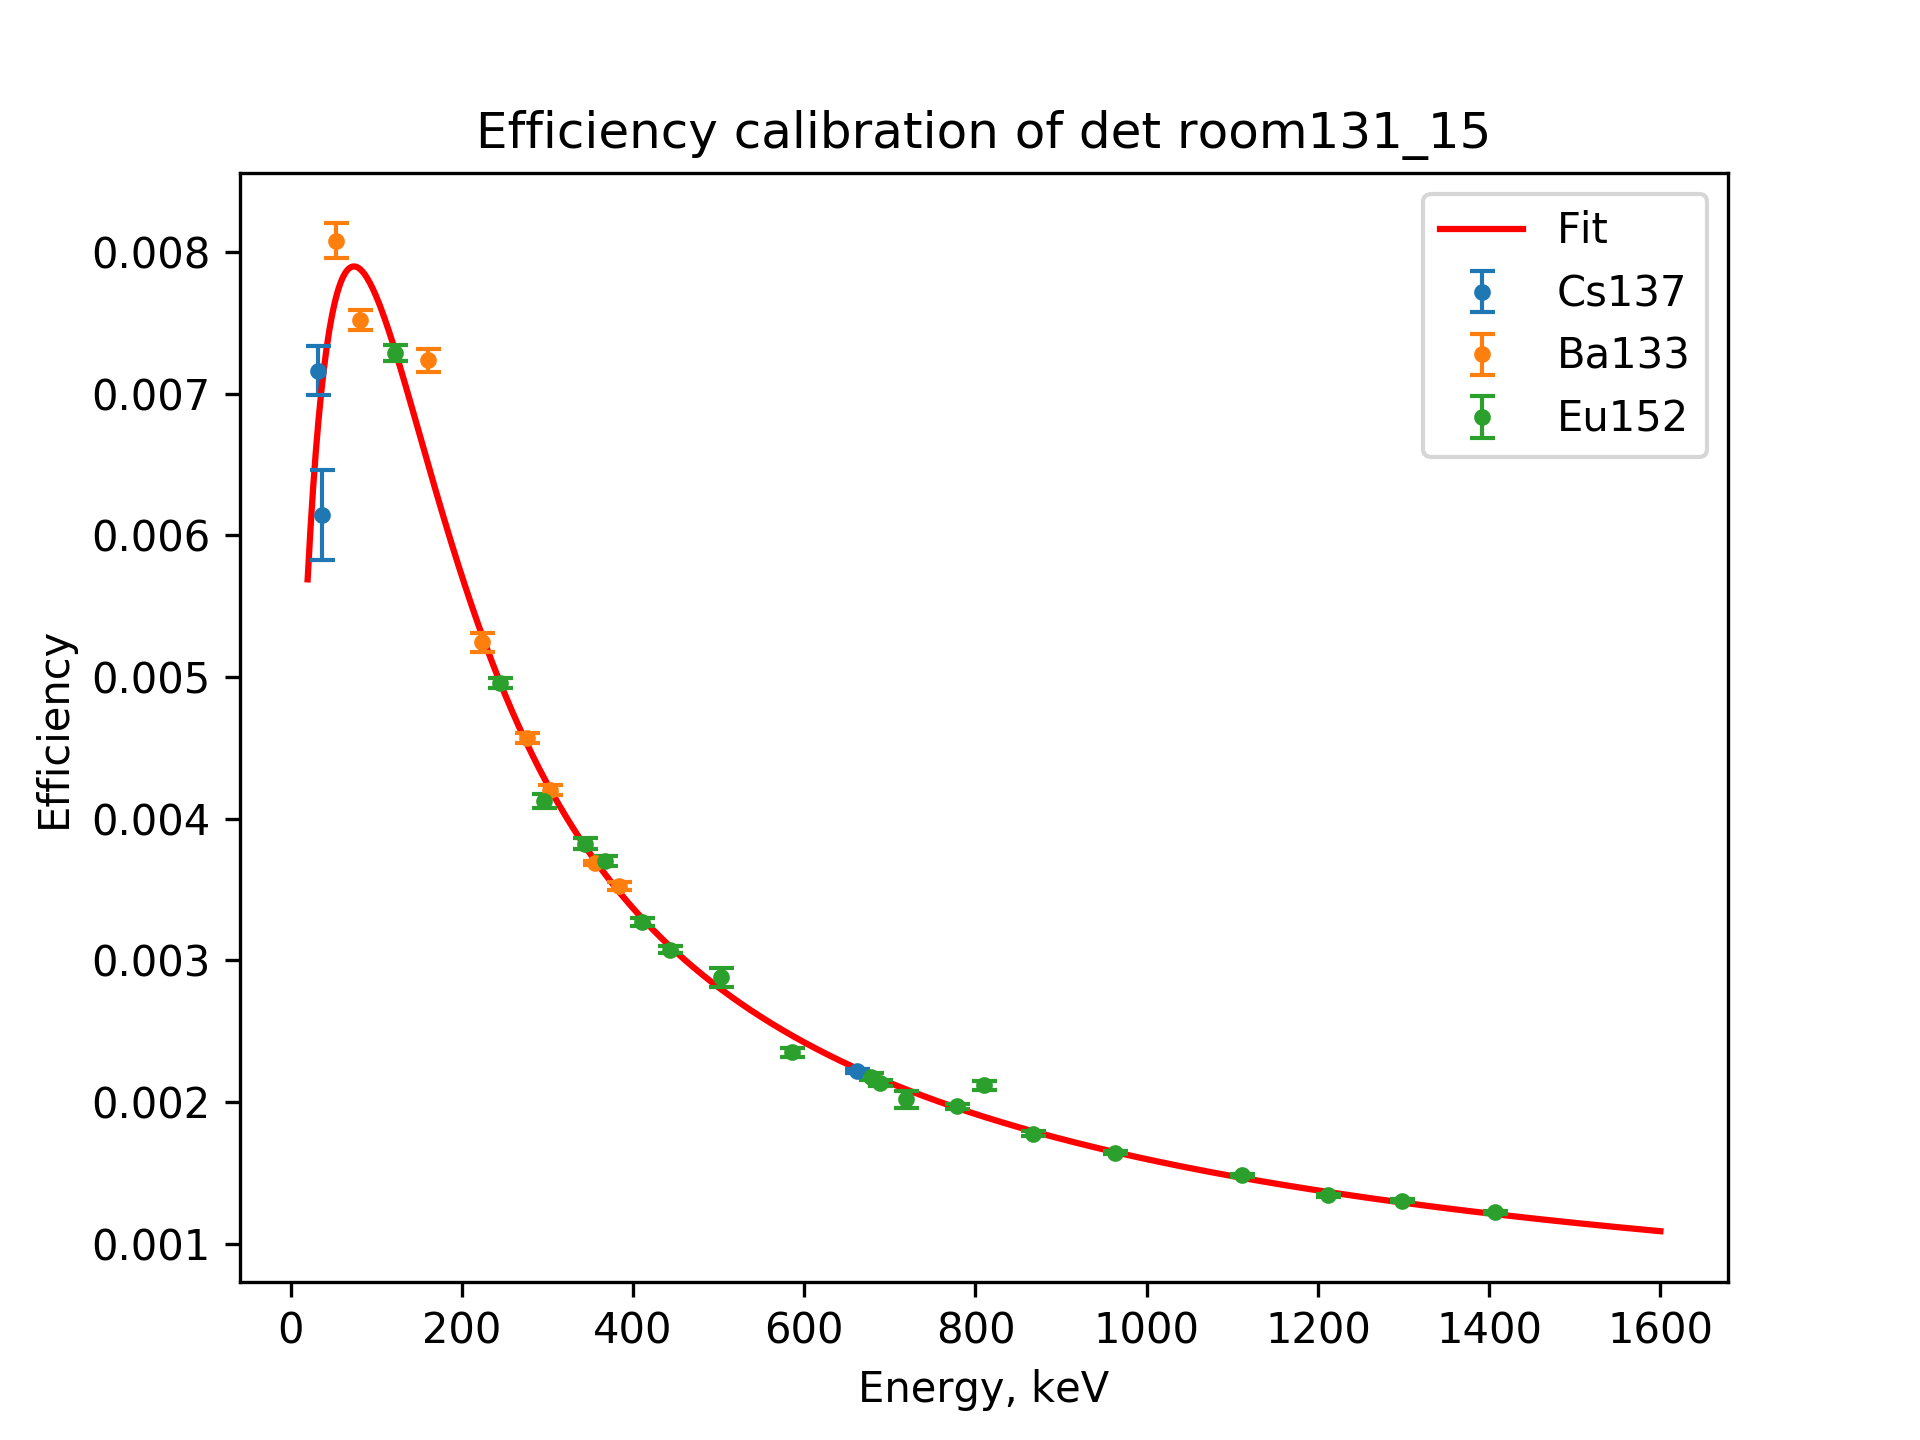
\includegraphics[width=8cm]{Experiment/room131_15.png}
    \caption{An example of an efficiency curve}
    \label{fig:efficiency_curve}
\end{figure}

\begin{comment}
\begin{table}[]
    \centering
    \caption{The calibration point sources along with gamma lines used. * indicates that the value has been averaged over two peaks with similar energy. For the intensity its just added together. }
    \begin{tabular}{|cc|cc|cc|}
        \hline
        
         \multicolumn{2}{|c}{\makecell{^{137}Cs}} & \multicolumn{2}{c}{\makecell{^{133}Ba}} & \multicolumn{2}{c|}{\makecell{^{152}Eu}}\\
         %\hline 
         \Xhline{2\arrayrulewidth}
         \makecell{E_\gamma}& \makecell{I_\gamma}&\makecell{E_\gamma}& \makecell{I_\gamma}& \makecell{E_\gamma}& \makecell{I_\gamma}\\
         \hline
         \makecell{32.005^*} & \makecell{5.63\%^*} & \makecell{53.1622} & \makecell{2.14\%} & \makecell{121.7817} & \makecell{28.53\%}\\
         
         \makecell{36.3405^*} & \makecell{1.02\%^*} & \makecell{80.9979} & \makecell{32.9\%} & \makecell{244.6979} & \makecell{7.55\%}\\
         
         \makecell{661.657} & \makecell{85.10\%} & \makecell{160.6120} & \makecell{0.638\%} & \makecell{295.9387} & \makecell{0.440\%}\\
         
          &  & \makecell{223.2368} & \makecell{0.453\%} & \makecell{344.2785} & \makecell{26.5\%}\\
         
          &  & \makecell{276.3989} & \makecell{7.16\%} & \makecell{367.7891} & \makecell{0.859\%}\\
         
          &  & \makecell{302.8508} & \makecell{18.34\%} & \makecell{411.1165} & \makecell{2.237\%}\\
          
          
          & \textcolor{red}{FINISH IF INCLUDING} & \makecell{302.8508} & \makecell{18.34\%} & \makecell{411.1165} & \makecell{2.237\%}\\
  
        %\makecell{^{137}Cs} & \makecell{^{133}Ba} & \makecell{^{152}Eu} \\
        \hline 
   
        \hline
    \end{tabular}
    \label{table:calibration_gammas}
\end{table}

\begin{table}[]
    \centering
    \caption{Table shows the geometry of the different detectors. }
    \begin{tabular}{|c|c|c|}
        \hline\textbf{}
        Detector & Geometry & Dimension \\
        \hline 
        \makecell{Detector 1} & \makecell{..} & \makecell{..} \\
        \makecell{Detector 1} & \makecell{..} & \makecell{..} \\      
        \makecell{Detector 3} & \makecell{..} & \makecell{..} \\     
        \makecell{Detector 4} & \makecell{..} & \makecell{..} \\  
        \makecell{Detector 5} & \makecell{..} & \makecell{..} \\    
        \makecell{Detector 6} & \makecell{..} & \makecell{..} \\      
        \makecell{Detector 7} & \makecell{..} & \makecell{..} \\     
        \hline
    \end{tabular}
    \label{tab:detector_characteristics}
\end{table}
\end{comment}

\noindent 
\subsubsection{Energy and peakshape calibration}
Each spectra that was taken was analyzed using FitzPeakz\footnote{https://www.jimfitz.co.uk/fitzpeak.htm}. \textcolor{red}{Write about how the program identifies peaks (read the article). The main mechanism  to search for peaks.  Explain how the detectors were calibrated using energy and peak shape. Each detector was calibrated using a..... }


\subsection{Irradiaton of target stack}
The irradiation of the target stack included a tuning of the beam and one hour of irradiation. Before we could turn on beam, we had to pump down the tube to a vacuum, to not attenuate the beam. \textcolor{red}{check the vacuum in notes}


\subsection{Tuning of the beam}
Before irradiation, the beam was tuned to have the \textcolor{red}{correct energy and beam spot}. The first step was to visualize the beam spot. \textcolor{red}{A glass plate with a 1 cm cross in the center that was painted with phosphorus was placed in the end of the beam tube}. With a camera placed in Cave 0 (not in the beamline), we could visualize the beamspot in the control room. This way, it was possible to steer the beam to be perfectly centered, which was important for the following experiment which used small targets. The next step was to visualize the beam over the target stack, \textcolor{red}{to make sure that the beam did not converge/diverge, spread?}. Gafchromic film changes color when exposed to ionizing radiation. A film was placed in the front and in the back of the target holder, and exposed for a brief seconds. This was done a couple of times before we were satisfied with the beamspot. \\

\noindent 
The last part of the beam tuning was to find beam efficiency of transmission which was done measuring the current at the Faraday cup right after the cyclotron vaul (BS-2) and right before cave 0 (FC-01). BS-2 was measured to be 420 nA, and FC-01 was measured to be 285 nA. This gave a beam efficiency of transmission
\begin{equation*}
    \frac{FC-01}{BS-02}=67\%
\end{equation*}
\noindent 
\textcolor{red}{In reference, .... Se over notater en gang til!}
\begin{comment}
Faraday cup right after Cyclotron vault $$BS-2 = 420 nA$$, and right before cave 0 was $$FC-01=285 nA$$

That gives a beam efficiency of transmission 

$$\frac{FC-01}{BS-02}=67.9\%$$
\end{comment}
\subsection{The irradiation of the target stack}

Figure \ref{fig:stack} shows the targets stacked in the beam holder, and figure \ref{fig:tube} shows how it was placed in the beam tube. 

\begin{figure}
    \centering
    \begin{subfigure}[b]{0.3\textwidth}
        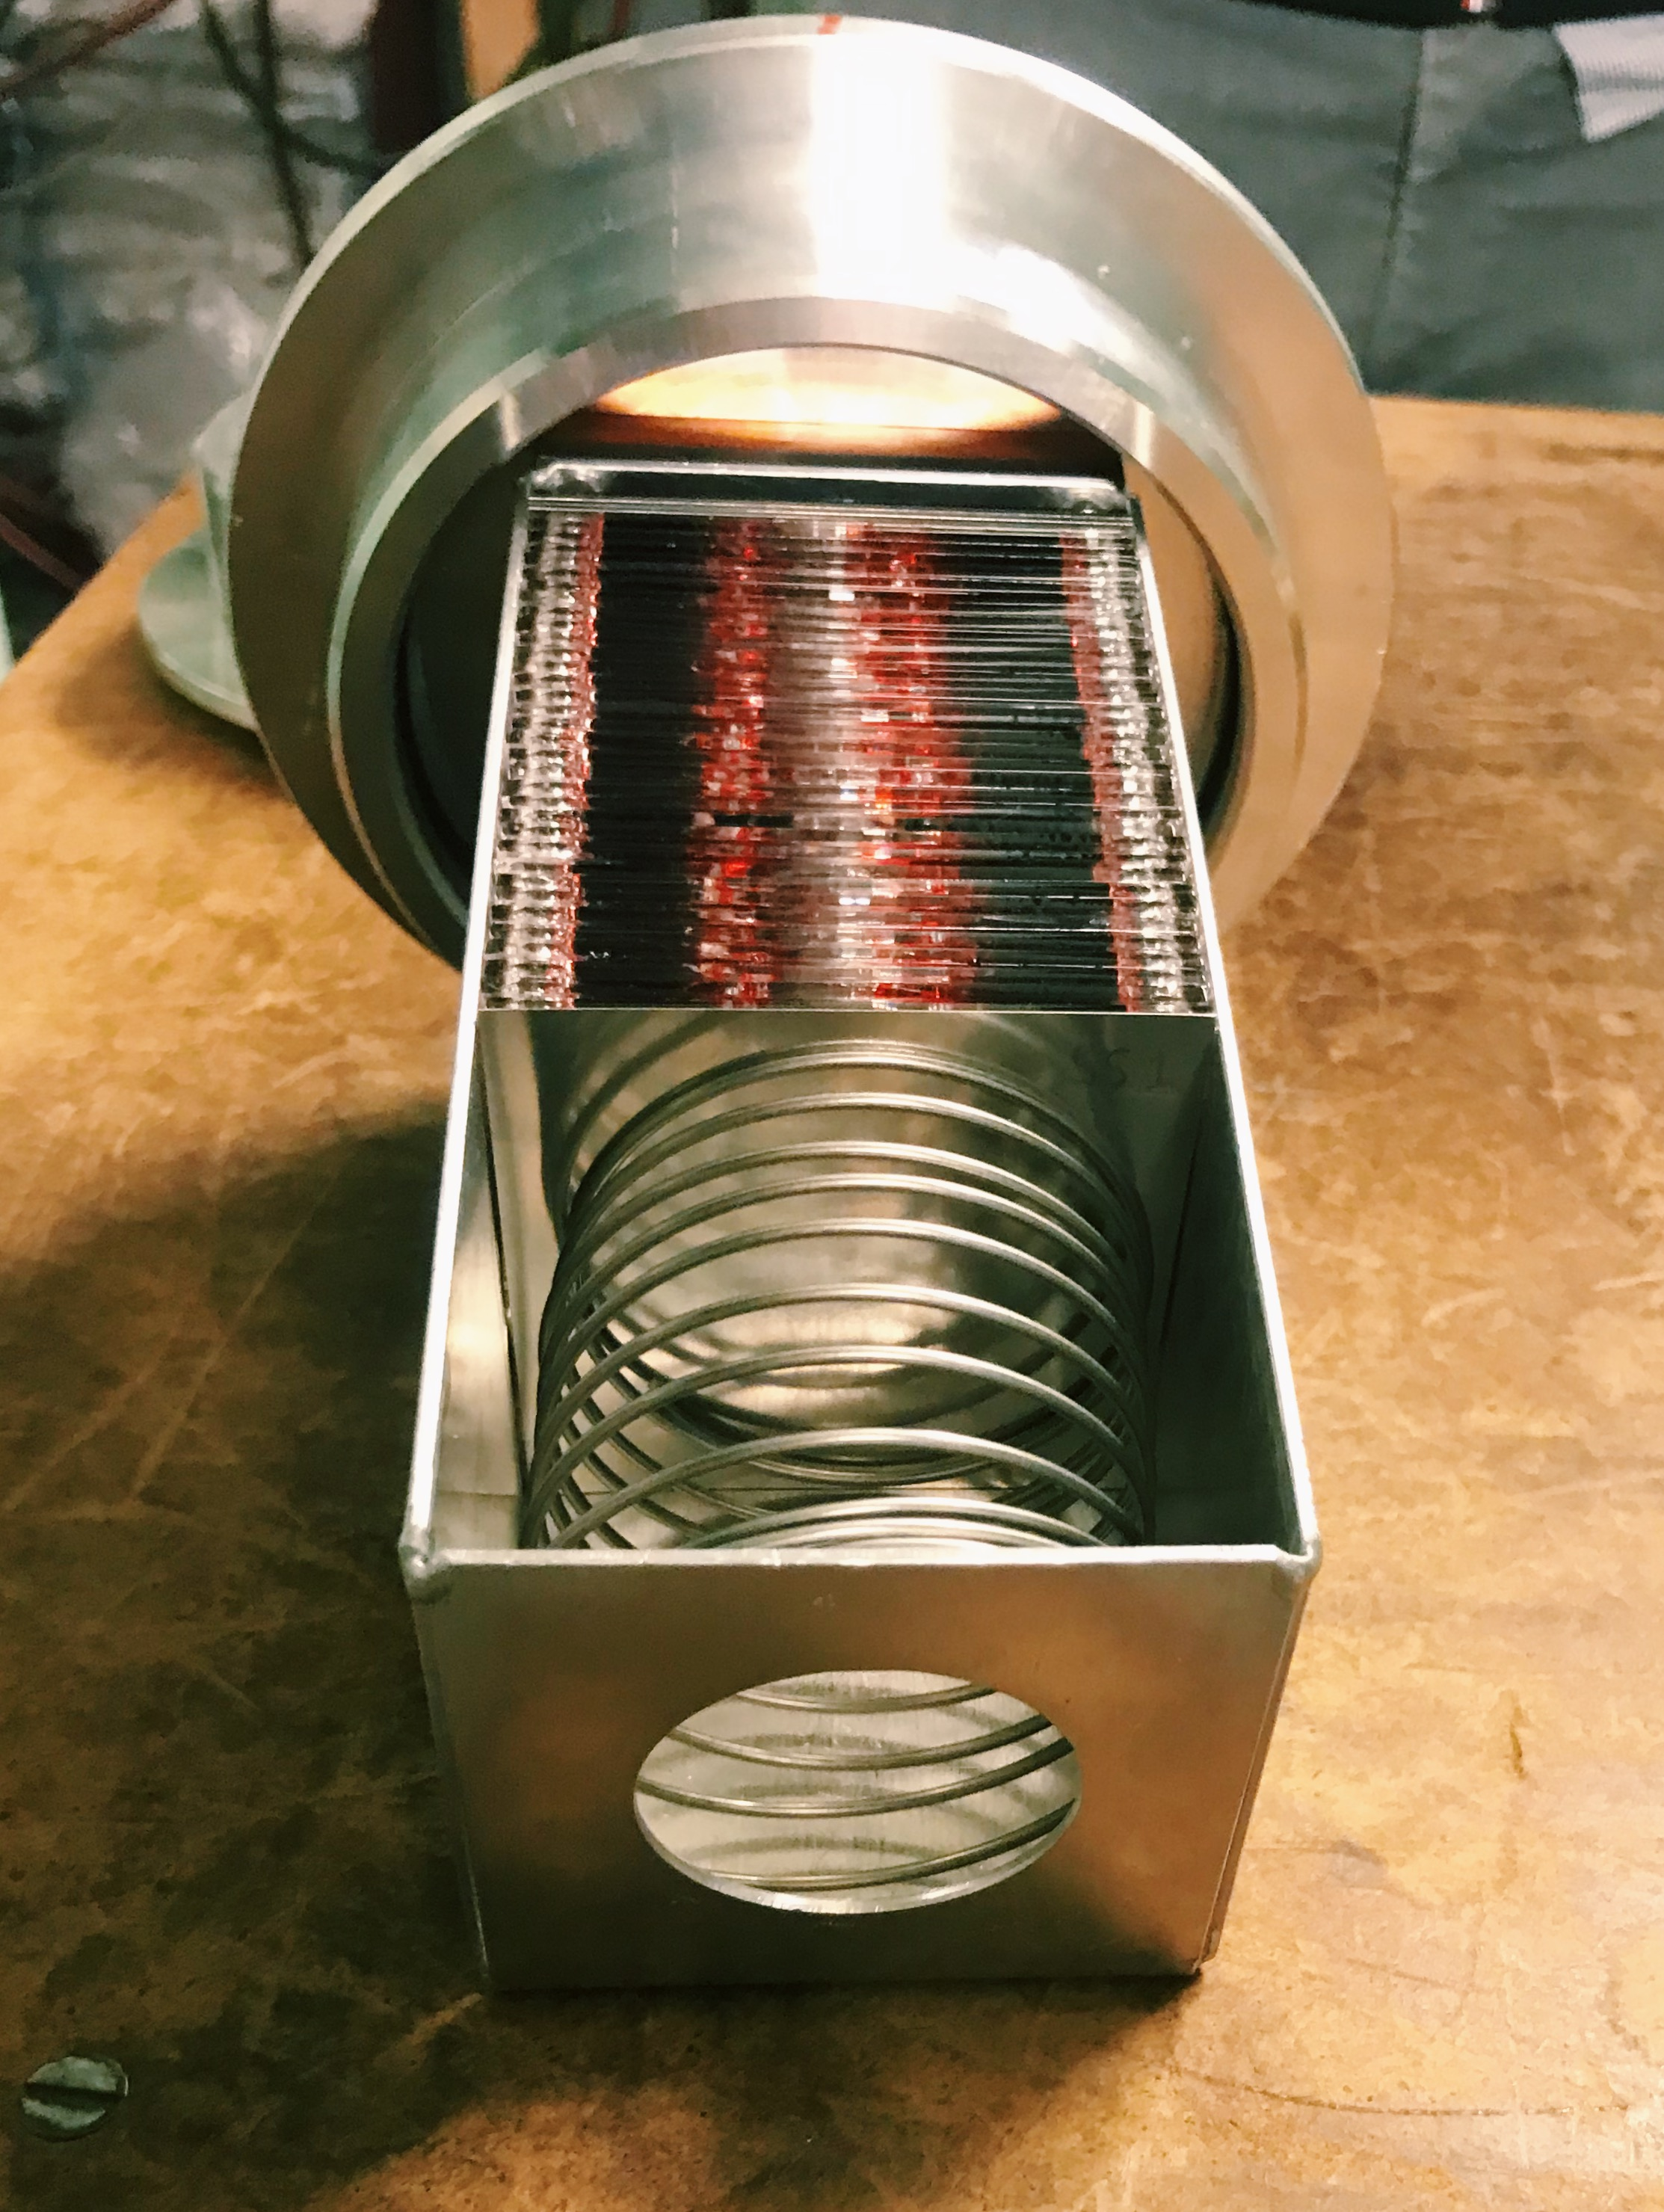
\includegraphics[width=\textwidth]{Experiment/stack.JPG}
        \caption{Foil stack}
        \label{fig:stack}
    \end{subfigure}
    ~ %add desired spacing between images, e. g. ~, \quad, \qquad, \hfill etc. 
      %(or a blank line to force the subfigure onto a new line)
    \begin{subfigure}[b]{0.3\textwidth}
        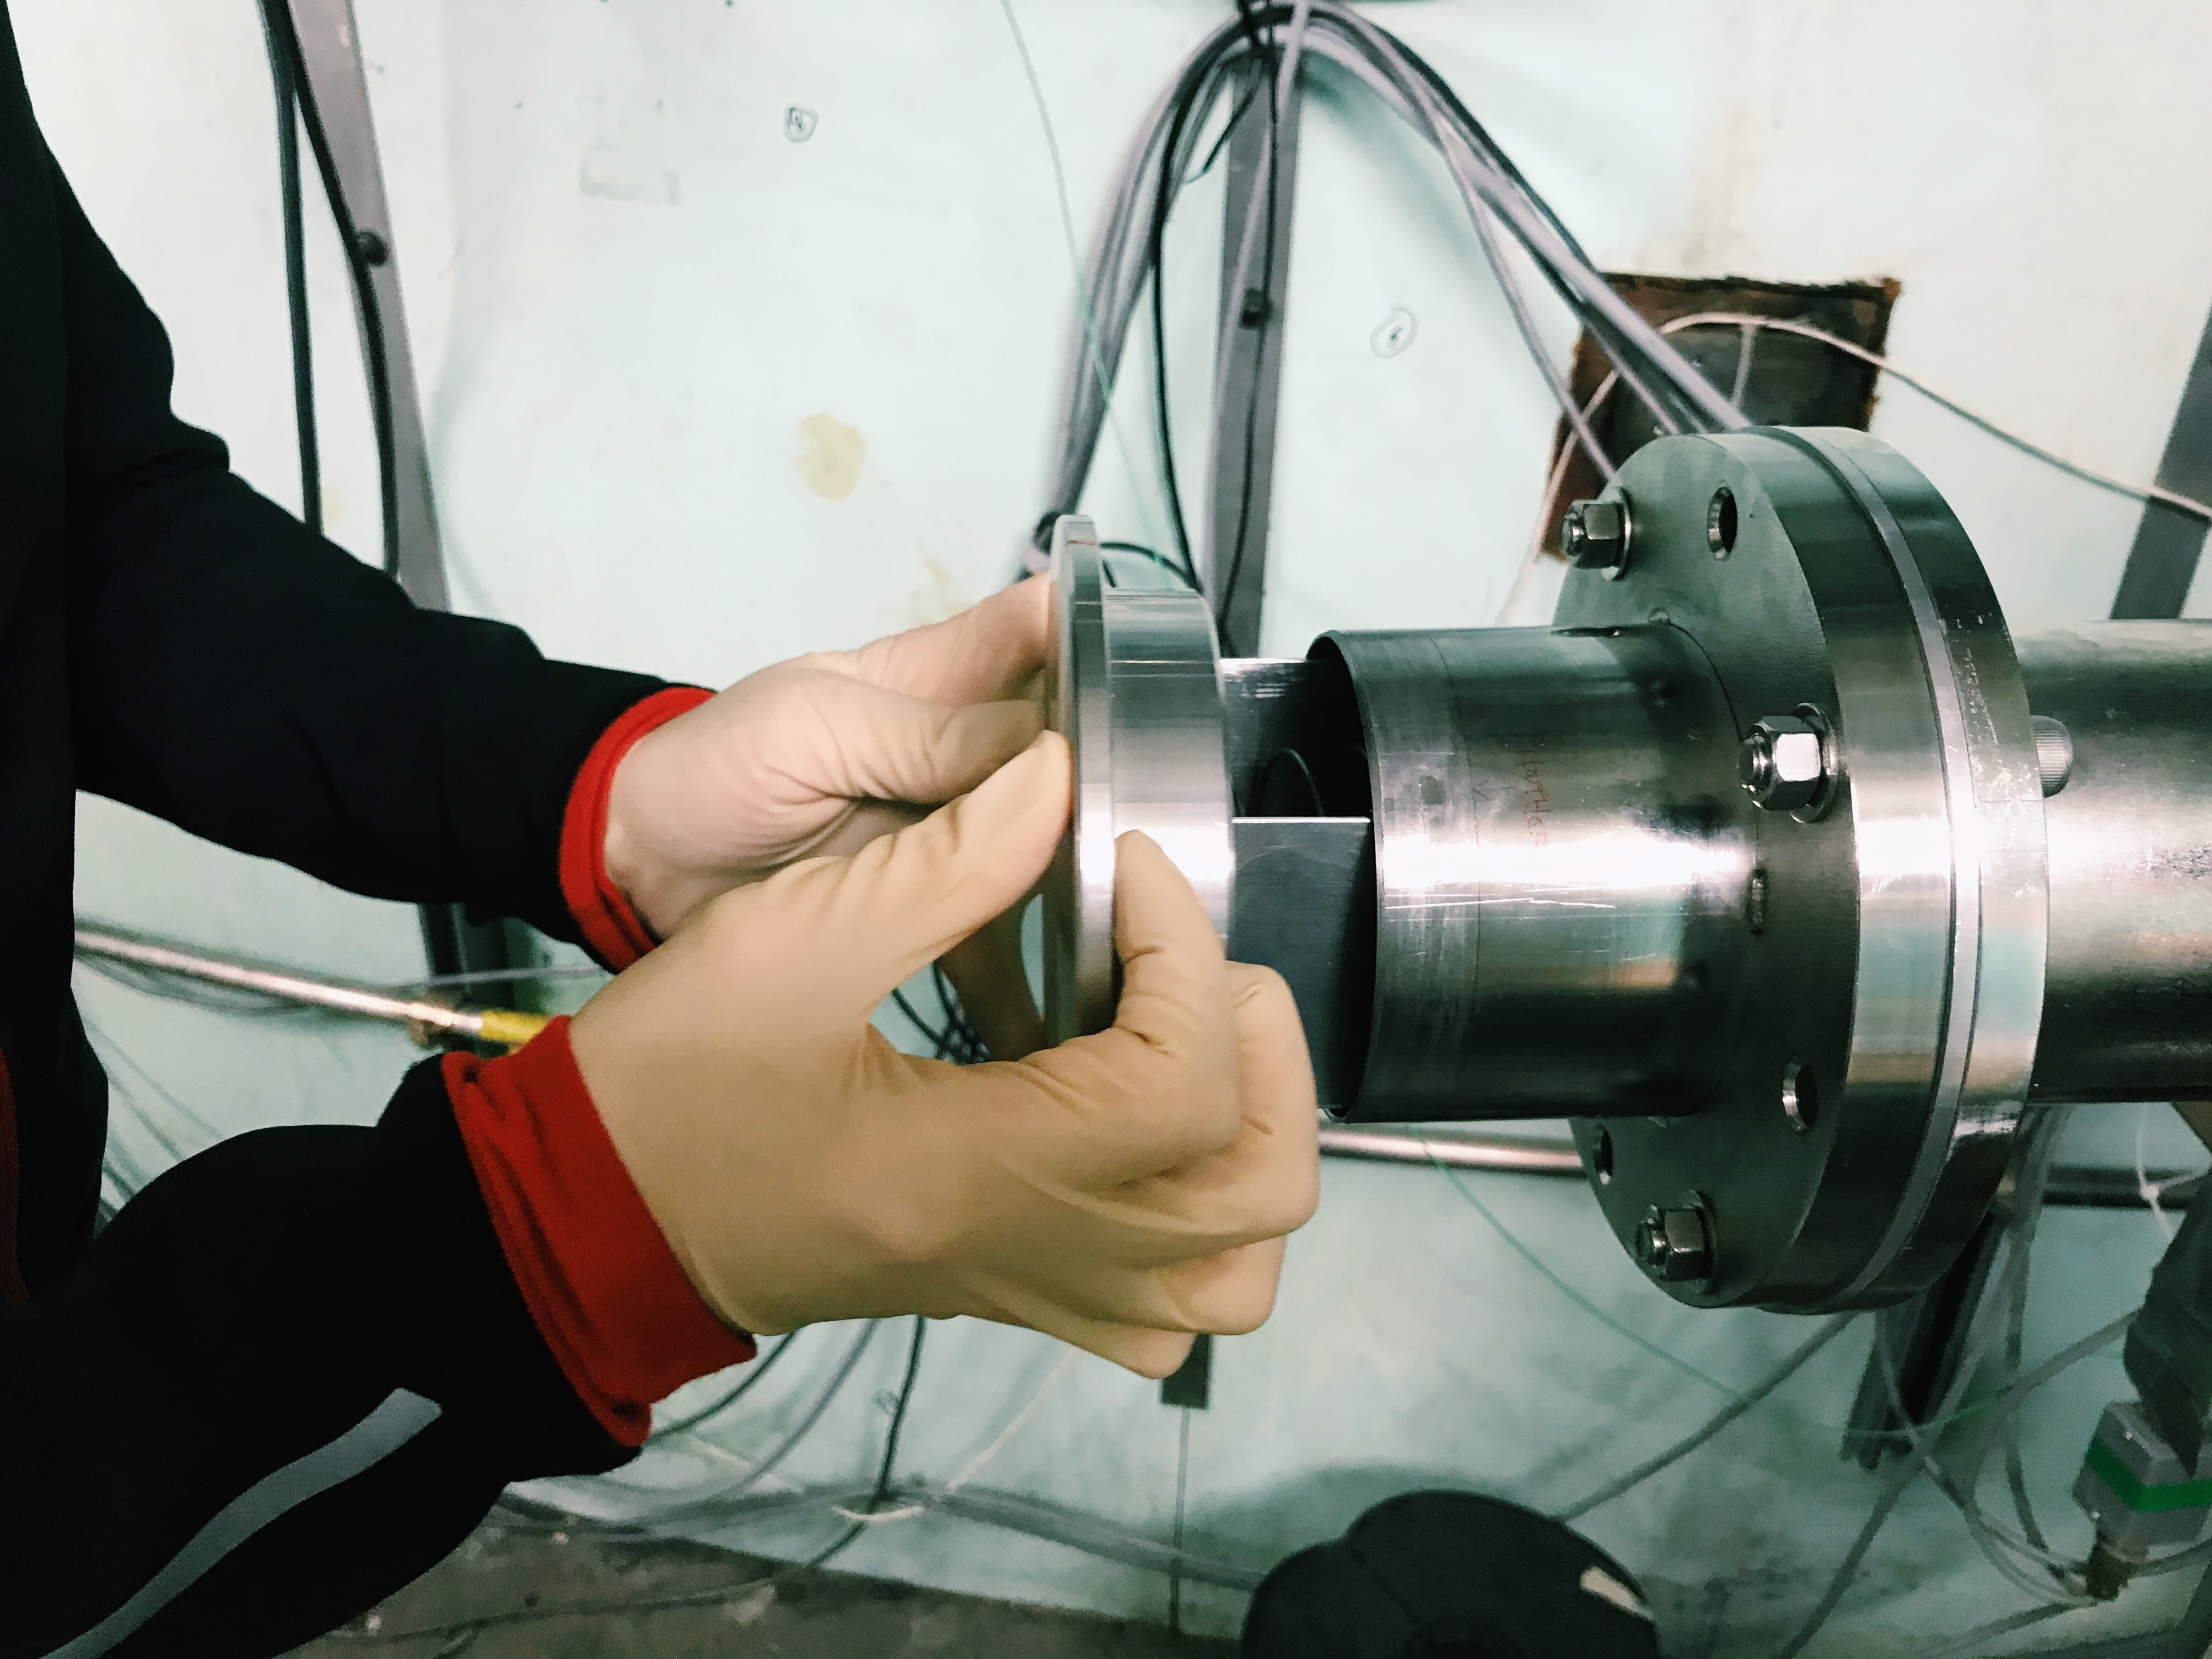
\includegraphics[width=\textwidth]{Experiment/tube.JPG}
        \caption{Beam tube}
        \label{fig:tube}
    \end{subfigure}
    ~ %add desired spacing between images, e. g. ~, \quad, \qquad, \hfill etc. 
    %(or a blank line to force the subfigure onto a new line)
    \caption{The figure shows the finished stacked target, on how it was placed in the tube. }\label{fig:finished_stack}
\end{figure}
\noindent
The target was irradiated for exactly an hour, and the current read of the beam integrator evenly, so assure it increases constantly. Beam current from beam integrator was 128.5 nA. Full scale amperes was $2\cdot 10^{-7} $ A. Right after end of beam, the targets were sealed in small plastic bags to avoid contamination, and counted immediately. 

%Setup (cyclotron, caves, bending magnets, faraday cup, beam integrator, vacuum)

\subsection{Beam profile}
The stainless steel in the front and back of the target stack was attached to a gafchromic film after irradiation, and we were able to measure the actual beamprofile throgh the target stack. Due to scattering, the beam profile tends to broaden through the stack. However, the beam was stopped in the stack, hence the profile that was measured is not valid for the spread in the stack. \textcolor{red}{Image-J\footnote{https://imagej.nih.gov/ij/download.html} is an imaging process program that allowed us to measure the beam spot, finding the relative intensity of the beam spot on the gafchromic films. Radius of the activity from stainless on gafchromic film is used in program Image-J. The intesity profile is Gaussian, and the beamprofile had a full width half maximum of ...., and in the back was .... }. By measuring the beam profile, we were able to build confidence in the size of the beam spot. The stainless steel \textcolor{red}{(which consist of )} has fast decay time. It emits beta particles. Since beta particles do not emit straight, thus the actual beam spot is slightly smaller.   

\subsubsection{Counting on detectors}
Since counts are based upon Poisson statistics, \textcolor{red}{check notes!!!}, the more counts each peak has, the better statistics. Right after end of beam all the foils were counted for a short period of time to assure to measure the short-lived activities. Since the decay-rate for these nuclei are high, the statistics were ok. The longer after end of beam, the longer counts to assure good statistics for the longer-lived products. The foils were counted for a period of 4 weeks after end of beam. Backgrond spectra were taken for each detector as well. This was especially important for detectors 1-6 which were located in cave 4C, where background was present. 


%\subfile{Introduction.tex}
%\subfile{Theory.tex}
%\subfile{Experiment.tex}
%\subfile{Analysis.tex}
%\subfile{Results.tex}
%\subfile{Discussion.tex}
%\subfile{Conclusion.tex}



\chapter{Analysis}\label{Chapter:Analysis}
\noindent

\subsection{Theory on radioactivity and production}

\subsection{Statistics}

\subsection{Efficiency curves}

\section{Gamma-ray spectroscopy}

FitzPeakz was used to find peaks in each spectra. From each spectrum, FitzPeakz provided a report file with the detector the correct detector calibration, datetime, livetime. For each peak, a peak energy, centre channel, full width half maximum of the peak, significanse, goodness of fit, peak area, uncertainty in peak area, gammas per second, and uncertainty in gammas per second, and an backgrond estimation was provided. The most important parameters were the energy and peak area ($N_C$), along with uncertainty in peak area. Gammas per second (also called count rate) was used get an indication of the rate of gammas, which in cases where backgrond was a question, a comparison along with background spectra could determine whether we needed to do a background subtraction.  \\

\noindent 
A program ran through all report files for each target, and gave a list of energies within a tolerance. If the energies were \textcolor{red}{within a tolerance of 0.5 keV??}, then energies were averaged.  On The Lund/LBNL Nuclear Data Search \footnote{http://nucleardata.nuclear.lu.se/toi/}, energies could be searched for within a tolerance for mass numbers ranging from the lowest stable isotope of the target - approximately 12 (which was calculated via the Q-value for possible reactions with 33 MeV deuterions) and up to two mass numbers (1 deuterions with one proton and one neutron) from the highest stable isotope. Each of the energies were tested and most assigned to a nucleus. 

\subsection{Background subtraction}

\noindent 
In a few number of cases, background subtraction was necessary, due to the presence of some nuclei in the background. \textcolor{red}{This was especially necessary for some isotopes of Cobalt, which are high in production for both nickel and iron. Other background??}. The general rule of thumb was only to use background subtraction when all gamma lines for the nucleus was also present in the background with a count rate of the same order. If it was only a shared gamma line, we would try to avoid using it at all. \\

\noindent 
The calculation was done the following way: 
Countrate is defined as the number of counts divided by the livetime of the spectrum, in units counts/second. 
$$C=\frac{N_C}{\Delta t_\text{live}}$$
The number of observed counts is the sum of the true gammas and the background. 
\begin{equation}
    C_\text{observed}=C_\text{true} + C_\text{background}
\end{equation}

\begin{equation}
 C_\text{observed}= \Big(\frac{N_\text{true} }{\Delta t_\text{live}} \Big)_\text{current spectrum}  + \underbrace{\Big( \frac{N_\text{background}}{\Delta t_\text{live}} \Big)_\text{background spectrum}}_\text{=constant}
 \end{equation} %_\text{background spectrum}


%\end{equation}


From above we have that 
\begin{equation}
    N_\text{observed}=C_\text{observed}\Delta t_\text{live} = \Delta t_\text{live}(C_\text{true}+C_\text{background})
\end{equation}
\begin{equation}
    C_\text{true} = C_\text{observed}-C_\text{background}
\end{equation}

Finally, the true number of counts is

\begin{equation}
    N_\text{true}=N_\text{obs}- (\Delta t_\text{live} C_\text{background})
\end{equation}


\subsection{Cross section}
\begin{equation} \label{eq:CS_ch3}
    \sigma(\langle E \rangle) = \frac{A_0}{N_T \Phi (1-e^{-\lambda \Delta t_\text{irr}})}
\end{equation}


\subsection{Activities}
\textcolor{red}{Make a table which includes the various gamma lines that were used in the experiment}

The following section is based on Krane chapter 6\footnote{https://faculty.kfupm.edu.sa/phys/aanaqvi/Krane-Ch-6.pdf}: \\

\noindent 
The activity of a radioactive nucleus is equal to the radioactive decay rate 

\begin{equation}
    A = \frac{dN}{dt} = -\lambda N
\end{equation}
\noindent where N is the number of nuclei, t is the time and $\lambda$ is the decay constant. If we assume a target of a stable nucleus, which is exposed to a particle beam which induces various nuclear reactions, the constant rate of production of a specific reaction is dependent on the number of target nuclei, the current of flux of the particle beam and the reaction cross section 
\begin{equation} \label{eq:prod_rate}
    R = N_T \Phi \sigma
\end{equation}
\noindent 
where R is the production rate, $N_T$ is the number of target nuclei, $\Phi$ is the beam current or flux, and $\sigma$ is reaction cross section. In the assumption of the production rate being a constant value, the number transformed target nuclei is small in comparison to the total number during the irradiation time. The number of produced nuclei from a specific reaction is thus 

\begin{equation}
    dN = Rdt -\lambda N dt
\end{equation}

\noindent which has the solution 

\begin{equation}
    N(t) = \frac{R}{\lambda} (1-e^{-\lambda t})
\end{equation}

\noindent The total activity produced is thus 
\begin{equation}
    A(t) = R(1-e^{-\lambda t})
\end{equation}

\noindent When a target is irradiated, the activity of the product nucleus will increase until \textit{secular equilibrium} is achieved, which is when the product rate and decay rate are constant. Hence it is not necessary to irradiate a target for more than 2-3 half lives. \\ 

\noindent It is common that a radioactive nucleus decay into another radioactive nucleus. Hence the daughter activity will increase due to feeding from the parent. For multiple decay, \textit{Bateman equation} is used describing the activity in nucleus n of the decay chain \textcolor{blue}{(Voyles2018)}.

\begin{equation} \label{eq:Bateman}
    A_n(t) = \lambda_n \sum_{i=1}^{n} \Big[ \Big(N_{i,0} \prod_{j=i}^{n-1}\lambda_j\Big) \cdot \Big( \sum_{j=i}^{n}\frac{e^{-\lambda_j t}}{\prod_{i\neq j}^{n}(\lambda_i - \lambda_j) }\Big) \Big]
\end{equation}

\noindent 
where $A_n$ is the activity of nuclei n in the decay chain, with the corresponding decay constant $\lambda_n$. The equation sums over all nuclei in the decay chain. $N_{i,0}$ is the initial number of nucleus i, and j is the nucleus which is feeding into nucleus i.




\subsubsection{End of beam activities}
From equation \ref{eq:CS_ch3}, we need to estimate the end of beam activity for each nuclei. The end of beam activities were estimated using curvefit of multiple gamma-rays measured at different time points after end of beam. The activity measured a time t is calculated using one gamma-ray
\begin{equation} \label{eq:activity_spectra}
    A(t)=\frac{N_C \lambda}{\epsilon I_\gamma (1-e^{-\lambda \Delta t_\text{live}})e^{-\mu\rho\Delta r/2}}
\end{equation}
\noindent
where $N_C$ is the number of counts observed in the peak, $\epsilon$ is the detector efficiency, $I_\gamma$ is the intensity of the gamma-line, $\lambda$ is the decay constant of the nucleus, $\Delta t_\text{live}$ is the livetime of the spectrum. \textcolor{red}{The term $e^{-\mu \rho \Delta r/2}$ is the attenuation of the foil which is taken from \textcolor{red}{XCOM}, and $\rho\Delta r$ is a correction term due to thin foils which are not point sources, where we assume that only half of the mass density is detected since there is some attenuation in the foil as well.?????}.\\

\noindent 

\begin{enumerate}
    \item Activity 
    \item Uncertainty 
    \item Cumulative vs independent 
    \item False peaks
    \item Shared peaks and feeding. 
\end{enumerate}

\noindent
The scipy-curvefit method takes in all activities and uncertainties and minimizes the $\chi^2$ per degree of freedom, with an uncertainty weighting favouring the lowest uncertainties. \\

%\noindent 
%A decay chain is a decay where a parent product decays into a chain of daughter products, via $\alpha$ or $\beta$-decay. In the cases here, it is $\beta$-feeding. This means that the abundance of a particular isotope with feeding increases after the end of beam. 

\noindent 
If the first nucleus we observe in a decay chain has a parent that was produced but has too short half life to be observed, the first nucleus is reported as cumulative cross section. If there are independent observations in the next levels of the decay chain, they will be reported as independent and along with cumulative values.  

\noindent 
In the cases of this experiment, there was one step and two step decay that was calculated. With no feeding the simplest form of radioactive decay is sufficient

\begin{equation} \label{eq:radioactive_decaylaw}
    A(t)=\frac{dN}{dt}= \lambda N
\end{equation}

\noindent which simplies to when solving the differential equations

\begin{equation} \label{eq:onestep_activity}
    A(t) = A_0 e^{-\lambda t}
\end{equation}
\noindent 
In the cases of two step decay (n=2), the activity of the daughter is calculated from equation \ref{eq:Bateman}

\begin{equation} \label{eq:twostep_activity}
    A_2(t)= \lambda_ 2 \Big[ N_{1,0}\lambda_1 \frac{(e^{-\lambda_1} + e^{-\lambda_2})}{\lambda_1 - \lambda_2} + N_{2,0}e^{-\lambda_2 t}  \Big]
\end{equation}

\noindent from equation \ref{eq:radioactive_decaylaw}, the activity $A=\lambda N$, and two step decay is written as 

\begin{equation}
    A_2(t) = \frac{A_{1,0}\lambda_2}{\lambda_1-\lambda_2 } (e^{-\lambda_1 t} + e^{-\lambda_2 t }) + A_{2,0}e^{-\lambda_2 t}
\end{equation}

\noindent 
If the parent activity is known, the activity and cross section will be reported as independent and cumulative. If the parent activity is not known (due to lack of gamma lines for instance), the daughter activity and parent activity will be reported as cumulative. Figure \ref{fig:193mPt_activitycurve} shows an activity curve using single decay, for $^{193m}$Pt in foil 6. 

\begin{figure}
    \centering
    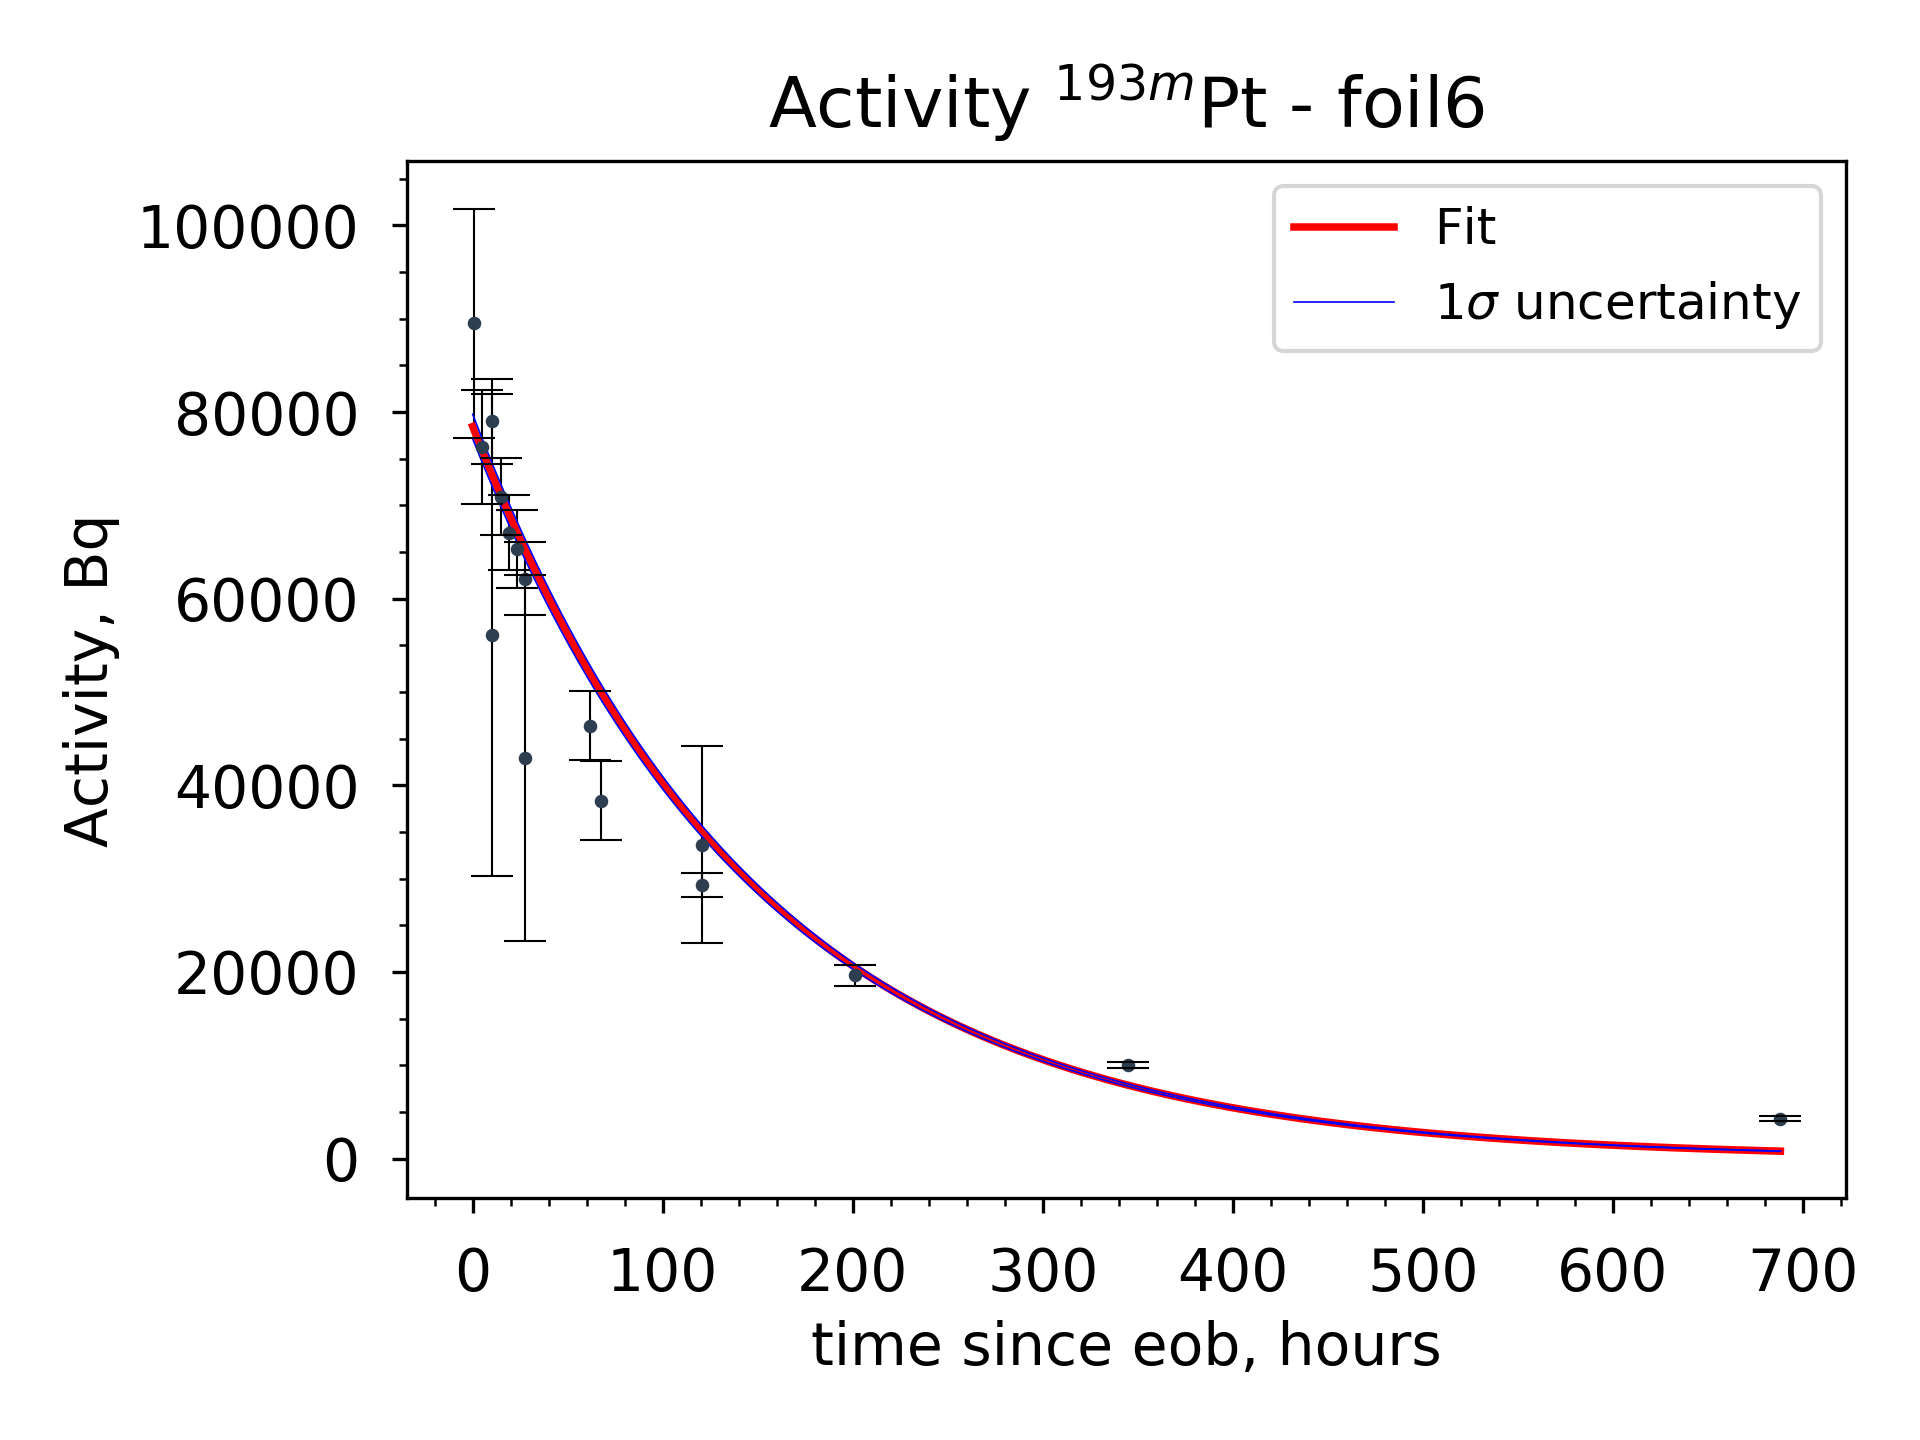
\includegraphics{Analysis/_activity_193mPt_677.png}
    \caption{An example of an activity curve using foil number 6 of $^{193m}$Pt with activities measured from the gamma ray spectroscopy using equation \ref{eq:activity_spectra}. The fitted curve is the single decay \textcolor{red}{Include two step decay also to give an example. } }  
    \label{fig:193mPt_activitycurve}
\end{figure}


\subsection{Beam Current}

The beam integrator gave a current of tube hitting the stack with $128.5$ nA. However, due to the large energy degradation in the energy stack, there will be a certain spread in the beam, following scattering. This is also the first experiment which have used deuterium on a stack of targets, so beforehand, we did not know how much deuteron break-up would affect the current throughout the stack. Reactions from the copper, nickel and iron foils were used as monitor reactions to estimate the weighted average beam current which was used in the cross section calculation in equation \ref{eq:CS_ch3}. Well-known cross sections from IAEA were used\footnote{$https://www-nds.iaea.org/medical/monitor_reactions.html$. Need to add citation for each datapoint used.}; $^{\text{nat}}$Fe(d,x)$^{56}$Co, $^{\text{nat}}$Ni(d,x)$^{56,58}$Co and $^{\text{nat}}$Cu(d,x)$^{62,63,64}$Zn. \textcolor{red}{This method provides a more sensitive beam current calculation}. \\ 

\noindent 
In order to calculate the cross sections, we need an accurate measure of the beam current. Thus, with well-known cross sections from the monitor reactions, we can estimate the beam current: 

\begin{equation} \label{eq:BC_nodiff}
    \Phi = \frac{A_0}{N_T (1-e^{-\lambda \Delta t_\text{irr}})\sigma(\langle E\rangle)}
\end{equation}

\noindent 
In cross section experiments\footnote{based on special curriculum, p. 14}, the suggested value is a \textit{flux average cross section}, which implies that the cross section is dependent on the flux-weighted average beam energy. One single foil thus provides one cross section measurement, with the energy uncertainty only being dependent on the energy distribution in each foil. For thin targets, we assume a stopping power $dE/dx=0$ (a good approximation for targets which are less than 50 mg/cm$^2$ \textcolor{red}{citation?}), hence we can replace the cross section in equation \ref{eq:BC_nodiff} with the normalized 

\begin{equation}
    \sigma(\langle E \rangle) = \frac{\int \sigma(\langle E \rangle) \frac{d\phi(\langle E \rangle)}{dE}dE}{\int \frac{d\phi(\langle E \rangle)}{dE}dE}
\end{equation}

\noindent where $\sigma(\langle E \rangle)$ is the well-known monitor cross section from IAEA, $\phi/dE$ is the differential deuterium fluence.  Using the above expression, beamcurrent can be written on the form 

\begin{equation}
    \Phi(\langle E \rangle) = \frac{A_0}{N_T (1-e^{-\lambda \Delta t_\text{irr}})\frac{\int \sigma(\langle E \rangle) \frac{d\phi(\langle E \rangle)}{dE}dE}{\int \frac{d\phi(\langle E \rangle)}{dE}dE}}
\end{equation}

\noindent 
The energy degradation was measured using NPAT's (nuclear physics analysis tool) Ziegler simulation. The code is based on Ziegler stoppingpower formalism and Monte Carlo simulations \textcolor{red}{Write more about npat, and what type of formalism its based on}. However, the large challenges to the simulation is to assign the correct energy bins. Especially, in energy ranges where the cross section is very sensitive to changes (changes rapidly as a function of energy). Figure \ref{fig:Ir_Flux_Distr} shows the energy distribution in the foils, where the flux is along the y-axis. The further back in the stack the harder it is to model, hence the full width half maximum increases

Thus, a need of variance minimization was necessary to assure that the correct energy bins was assigned to the stack. 

\begin{figure}
    \centering
    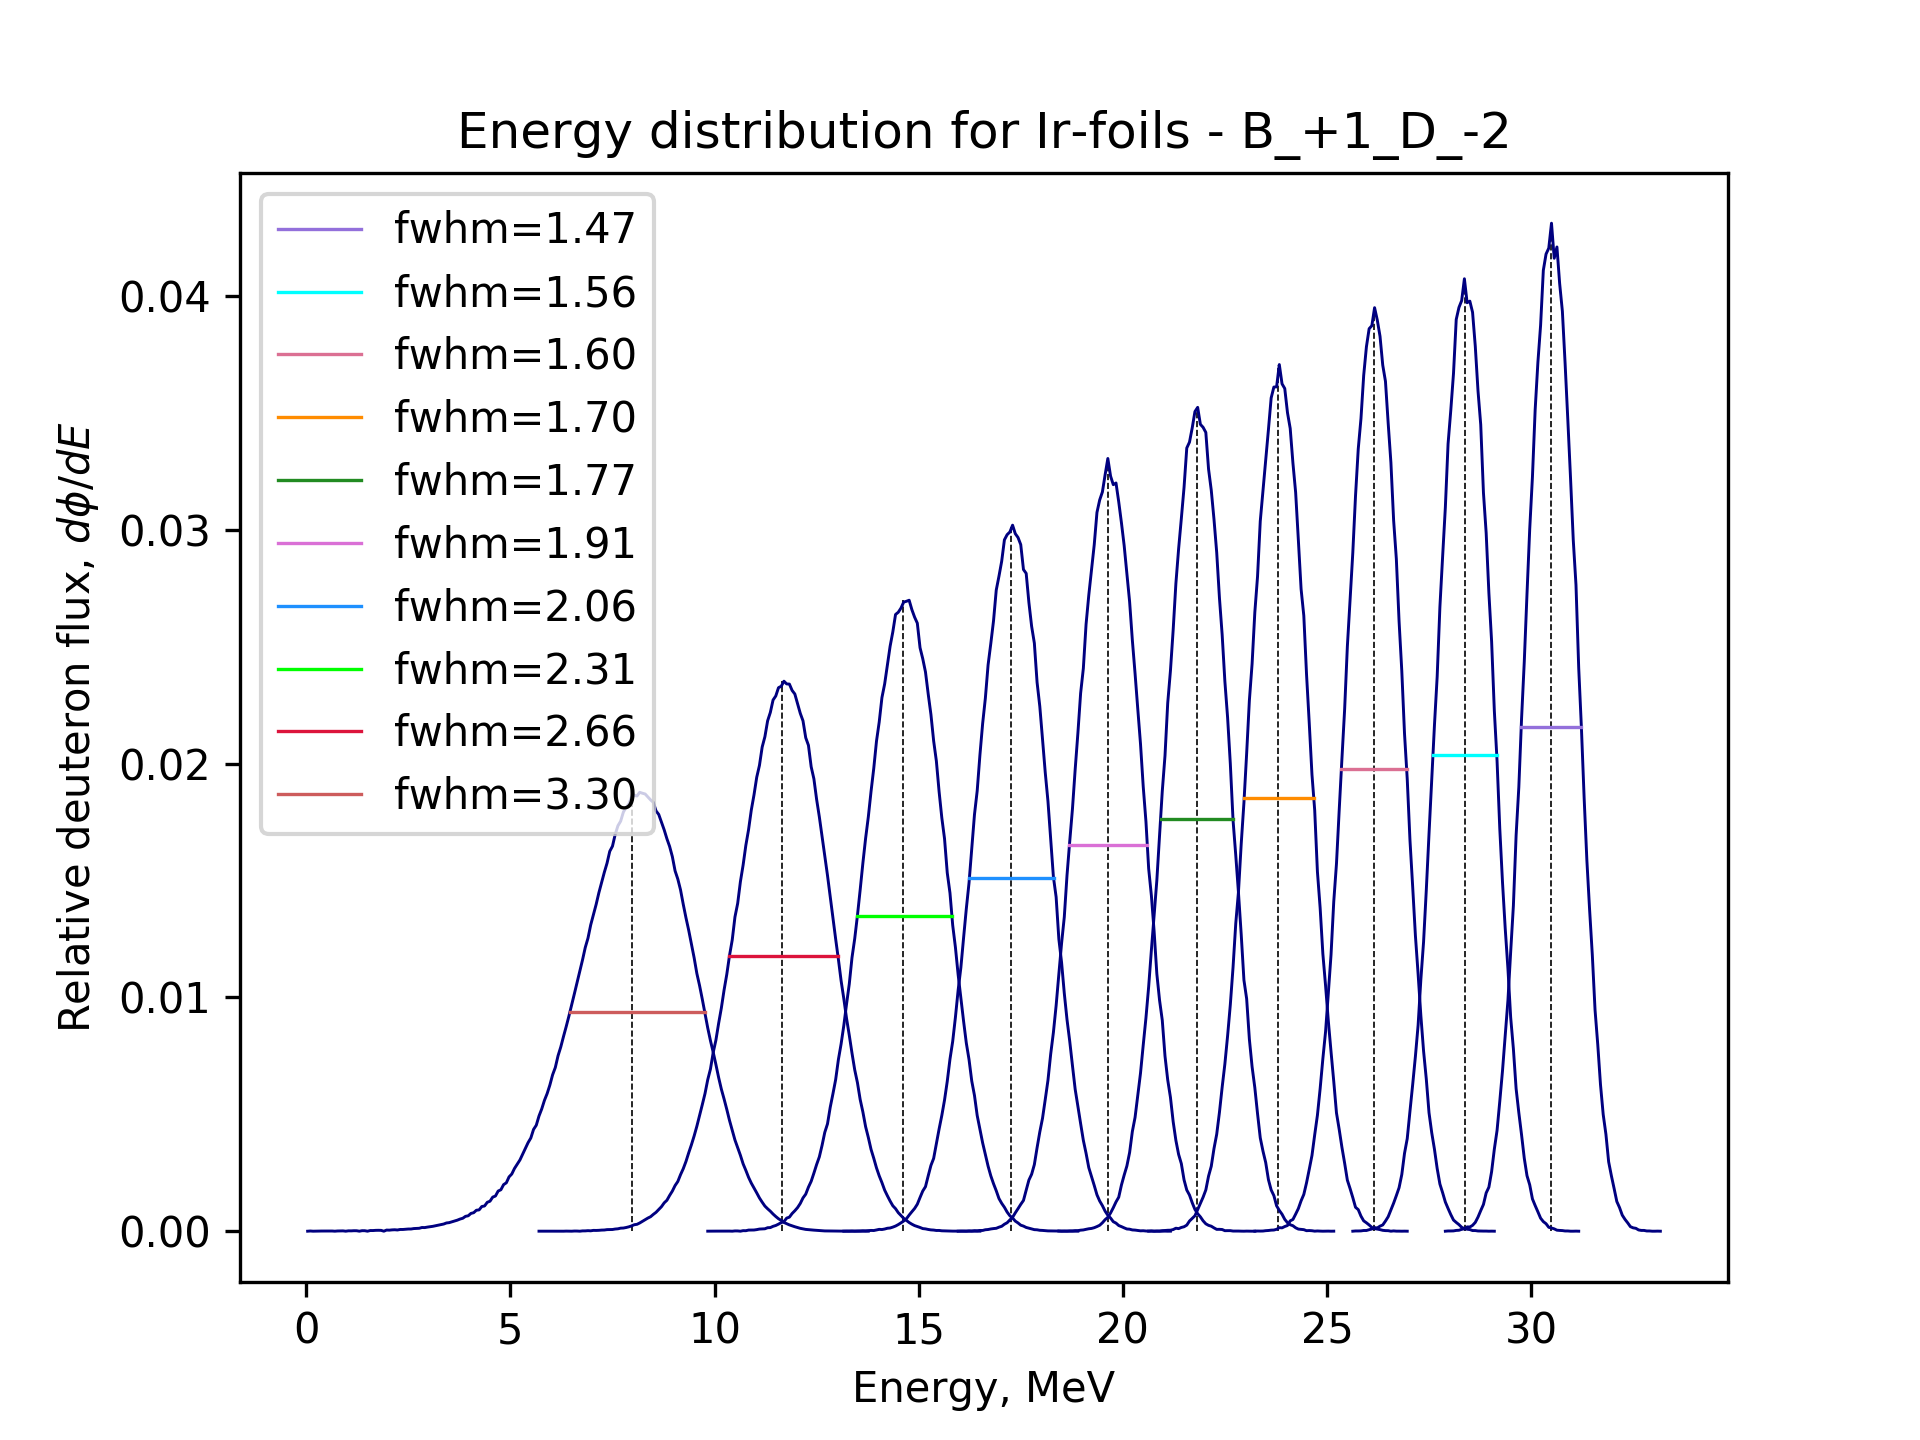
\includegraphics{Analysis/Ir_flux_distribution_B_+1_D_-2.png}
    \caption{The energy distribution of the iridium foils throughout the stack. \textcolor{red}{Should be very sure that it the beamcurrent in the end. } }
    \label{fig:Ir_Flux_Distr}
\end{figure}


\subsection{Variance minimization}
Ziegler files provides a set of energy and fluxes through the different foils. 
Did a areal density and beam energy increase and dicrease to see how it affected the current. Gives an energy distribution. Show figures.  \\

$\chi^2$ is an estimation of the goodness of fit which weight includes weight of error. The value is divided on the number of degrees of freedom (essensially the number of parameters minus 1. \textcolor{red}{why?})
\begin{equation} \label{eq:chi_squared}
    \chi^2 = \sum_{i}^n \Big(\frac{ y_i - \overline{y}}{ \sigma_i} \Big)^2 
\end{equation}

\noindent 
The idea was to get an estimation of the values of $\chi^2$ over the different compartments (one compartment is one set of foils, for instance Ni01, Ir01, Fe01 and Cu01). Compartment 3, 6 and 9 was investigated to get an idea of the scaling parameter that gave lowest values. If we cared about the $\chi^2$ values at high energies (early in the stack), the currents tend to be bad in the back of the stack, due to scattering at compartment 3 being low. However, in compartment 3, we had 7 independent measurements of beam current which gave more data. In compartment 9, a lot of the currents were low due to most reactions being at the energy threshold. Hence compartment 6 was used, which had 5 measurements (61Cu, 56,58Co, 63,65Zn). 62Zn was below threshold, and iron did not have any foil in compartment 6. The compartment can be seen in figure \ref{fig:varmin_comp6}. 

\begin{figure}
    \centering
    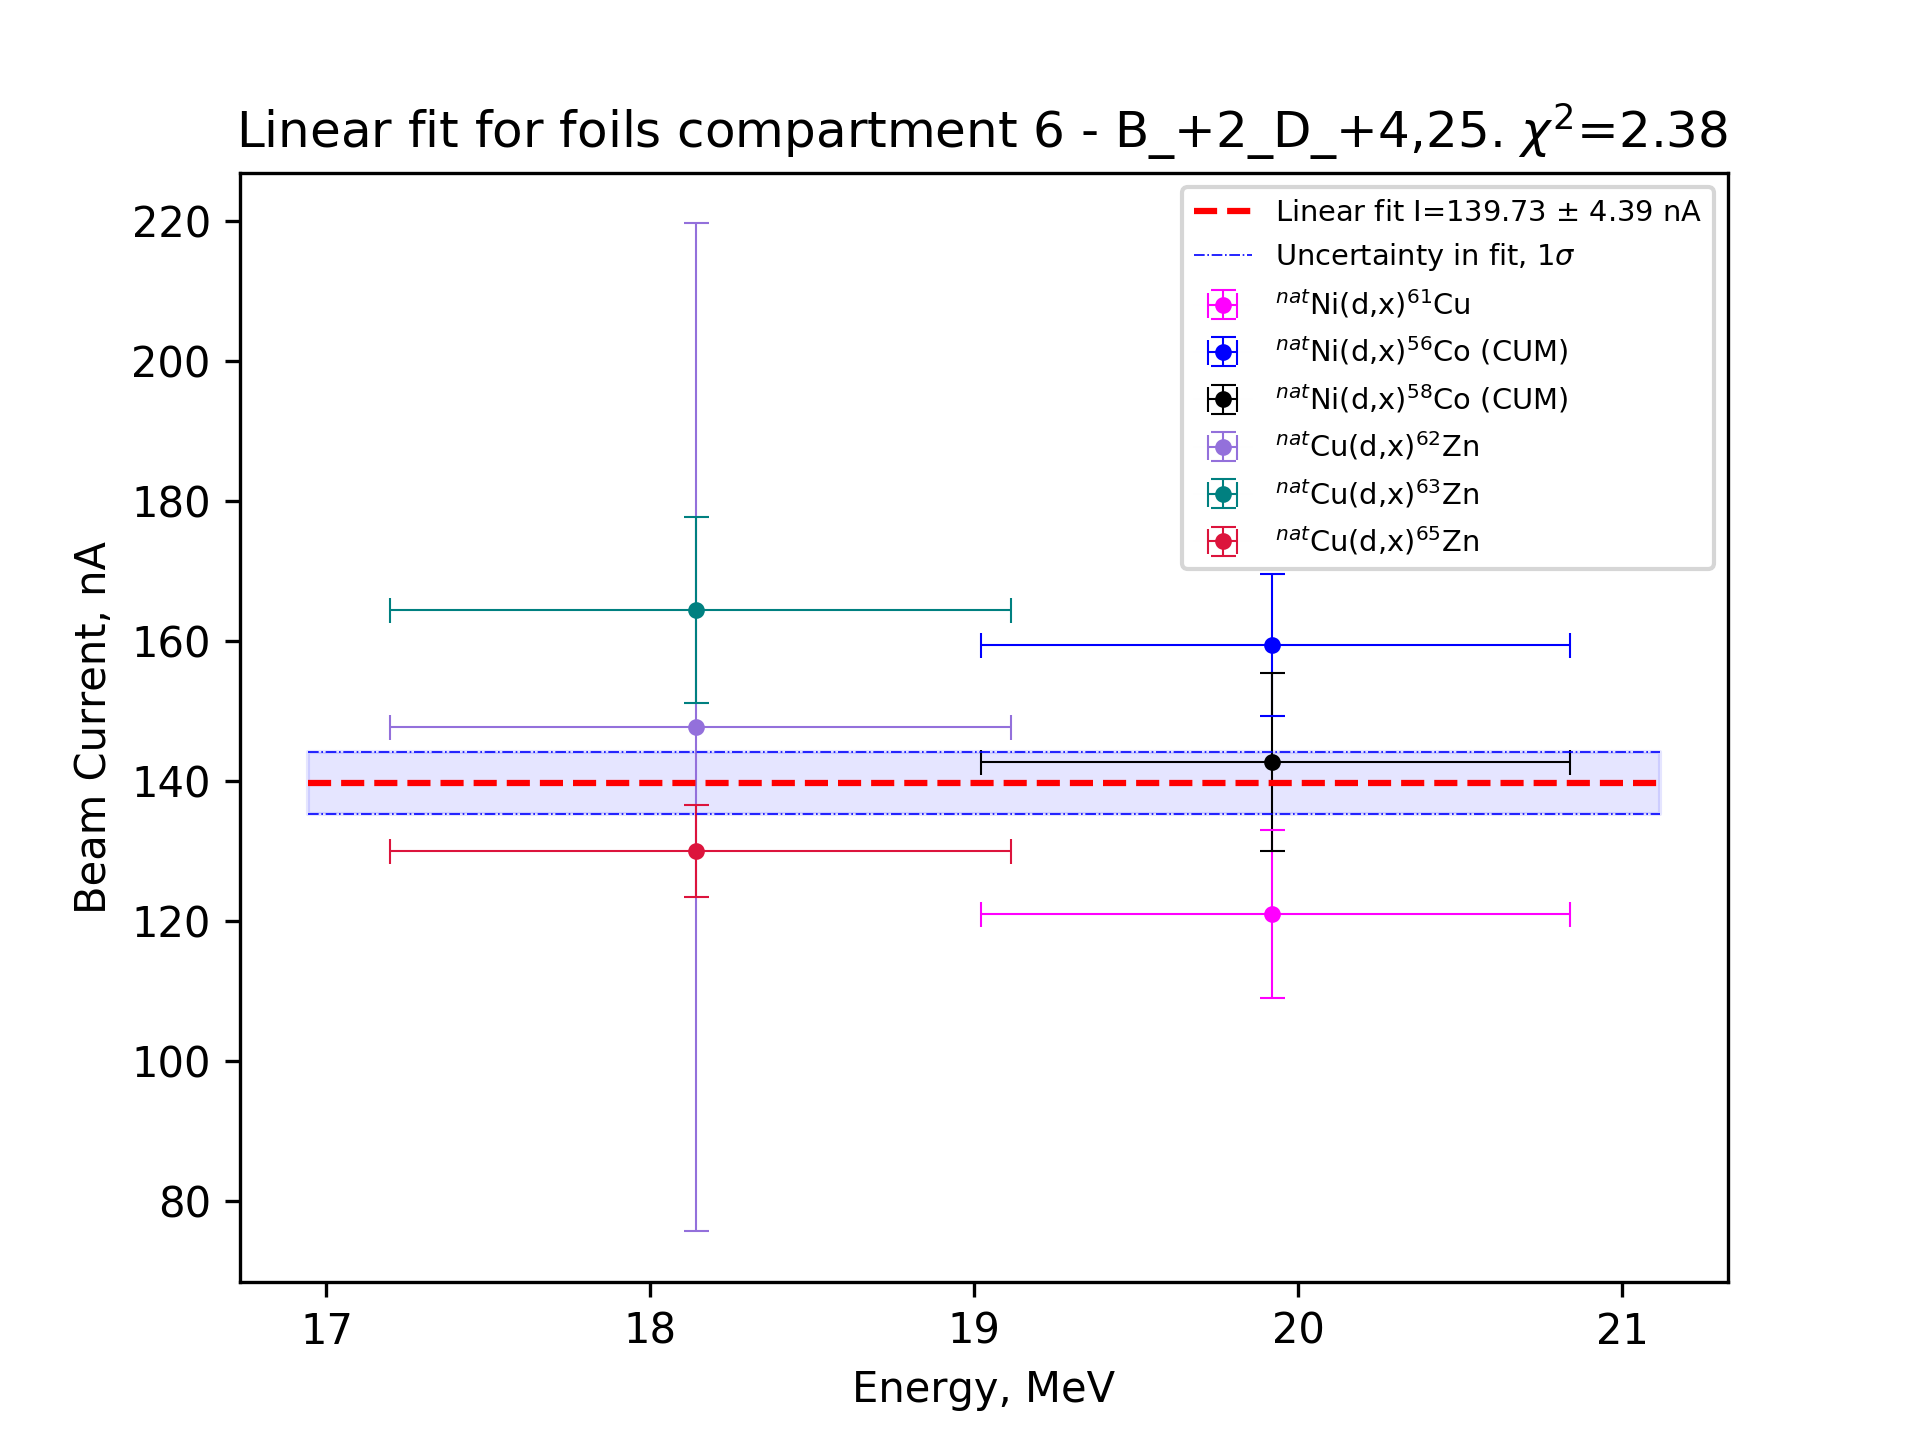
\includegraphics{Analysis/minimization_6_B_+2_D_+4,25.png}
    \caption{Variance minimization in compartment 6.}
    \label{fig:varmin_comp6}
\end{figure}

Assuming constant beam current in one compartment. Hence we can have a linear fit between the beam current measurements. With no current degradation, $y=mx+b$, m=0, b is initial guess of 128.5 nA. 

\begin{figure*}[t!]
  \centering
   \begin{subfigure}[t]{2\textwidth}
        \centering
        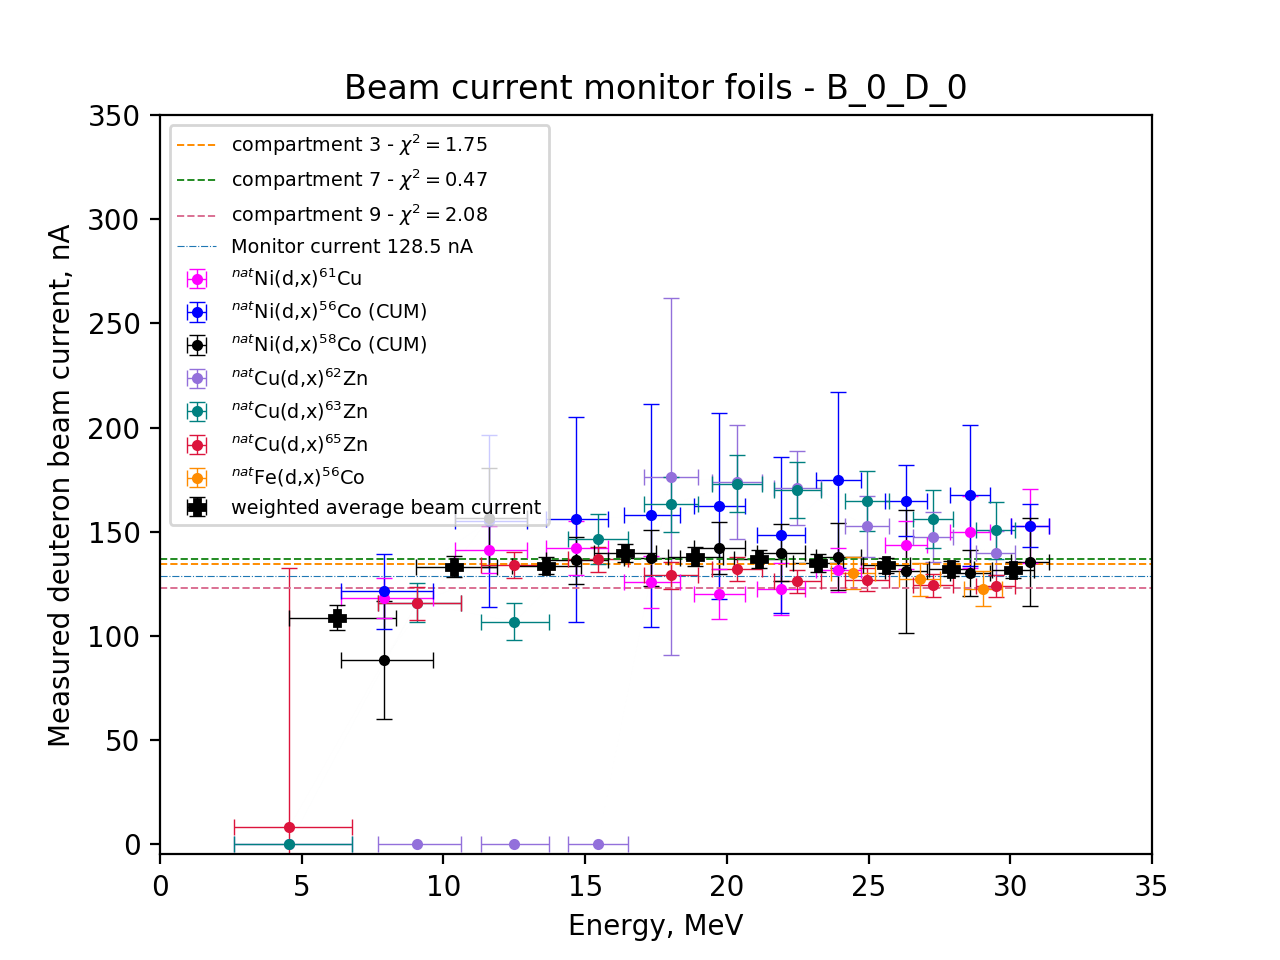
\includegraphics[height=1.2in]{Analysis/B_0_D_0.png}
        \caption{Before variance minimization}
    \end{subfigure}%
    \begin{subfigure}[t]{2\textwidth}
        \centering
        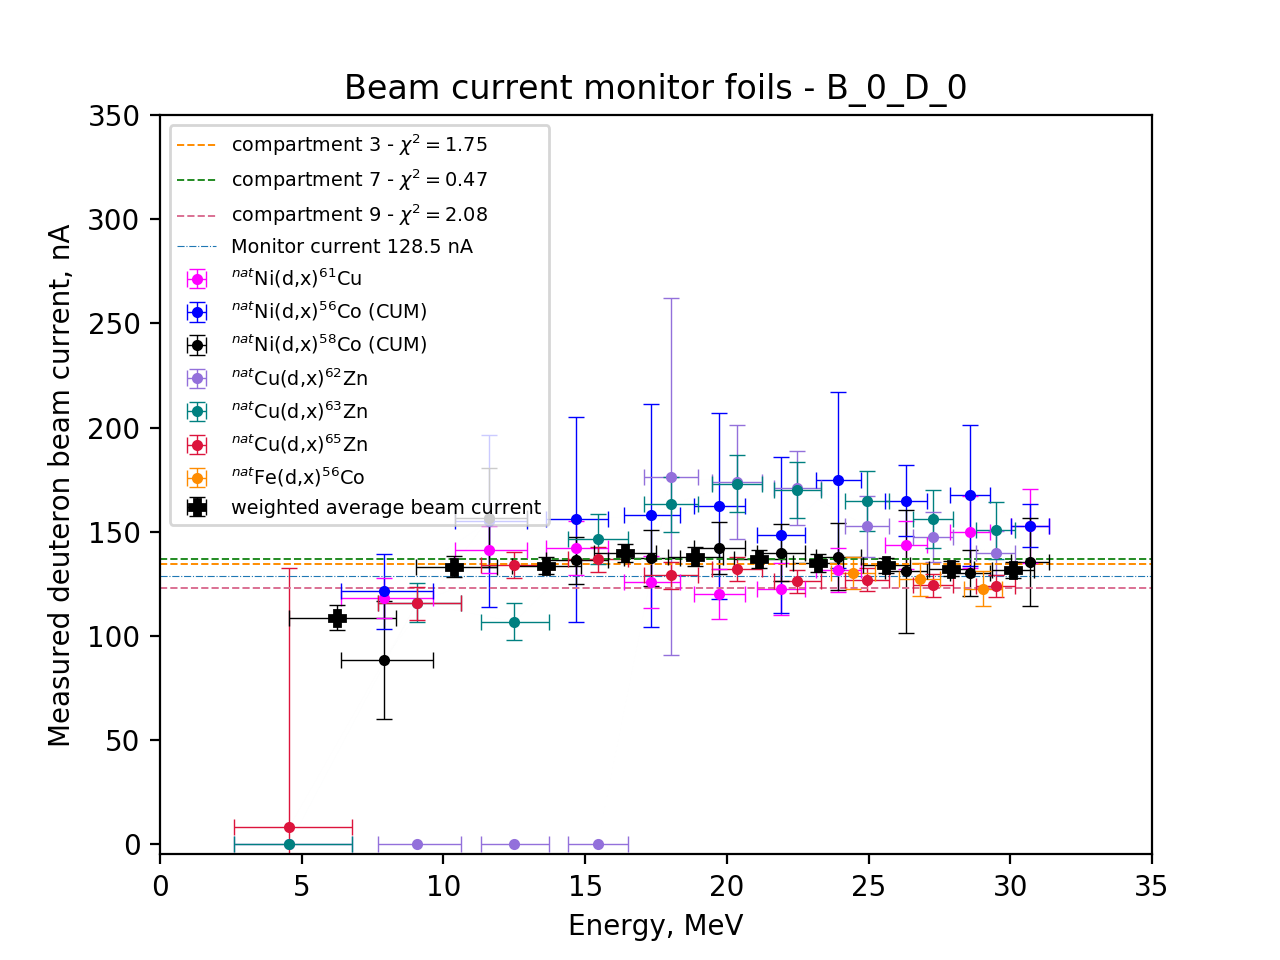
\includegraphics[height=1.2in]{Analysis/B_0_D_0.png}
        \caption{After variance minimization}
    \end{subfigure}
    \caption{Before, the current in the back of the stack is tending to be lower. The $\chi^2$ in the different compartments also tend to be higher. After variance minimization, the values for $\chi^2$ are smaller and the estimated current in each compartment agrees more with each other. We do not expect much of current degradation.}%
    \label{fig:varmin_beamcurrent}%}
\end{figure*}


%\begin{figure}%
%    \centering
%    \begin{subfigure}{.5\textwidth}
%    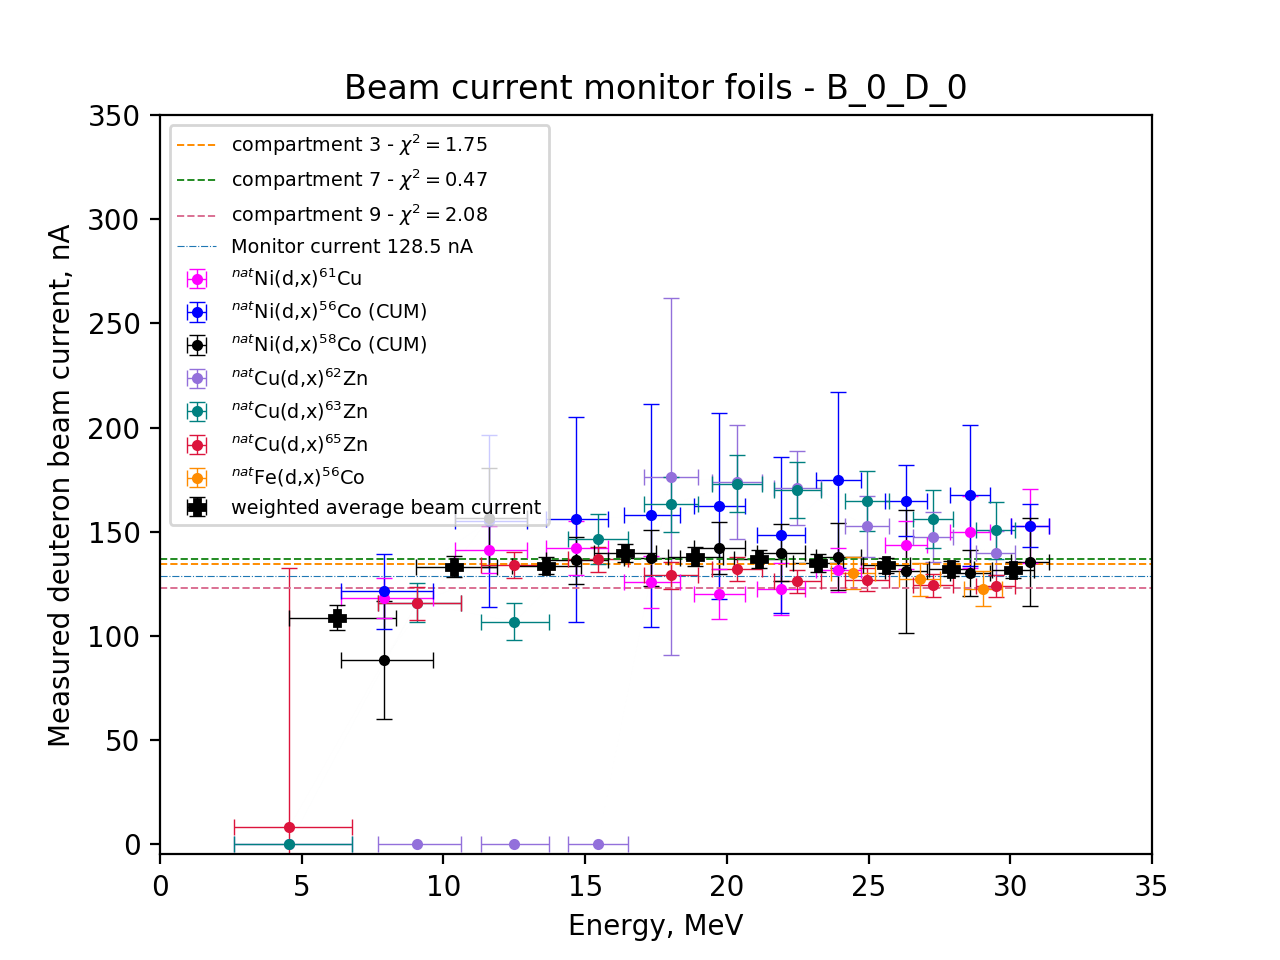
\includegraphics[width=8cm]{Analysis/B_0_D_0.png}
    %\subfloat[Before variance minimization]{{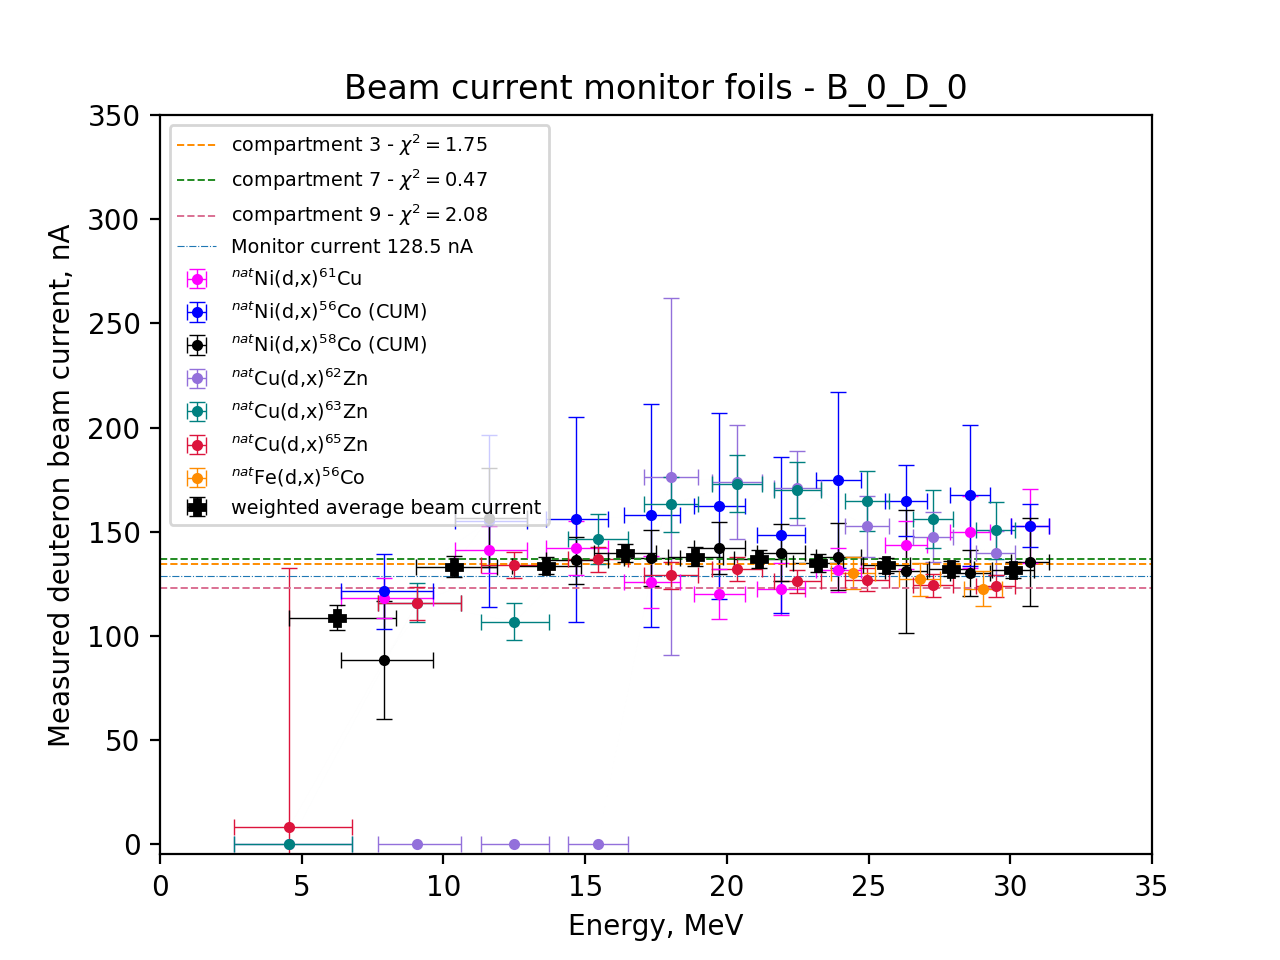
\includegraphics[width=8cm]{Analysis/B_0_D_0.png} }}%
%    \label{Before variance minimization}
%    \end{subfigure}
%    \begin{subfigure}{.5\textwidth}
%    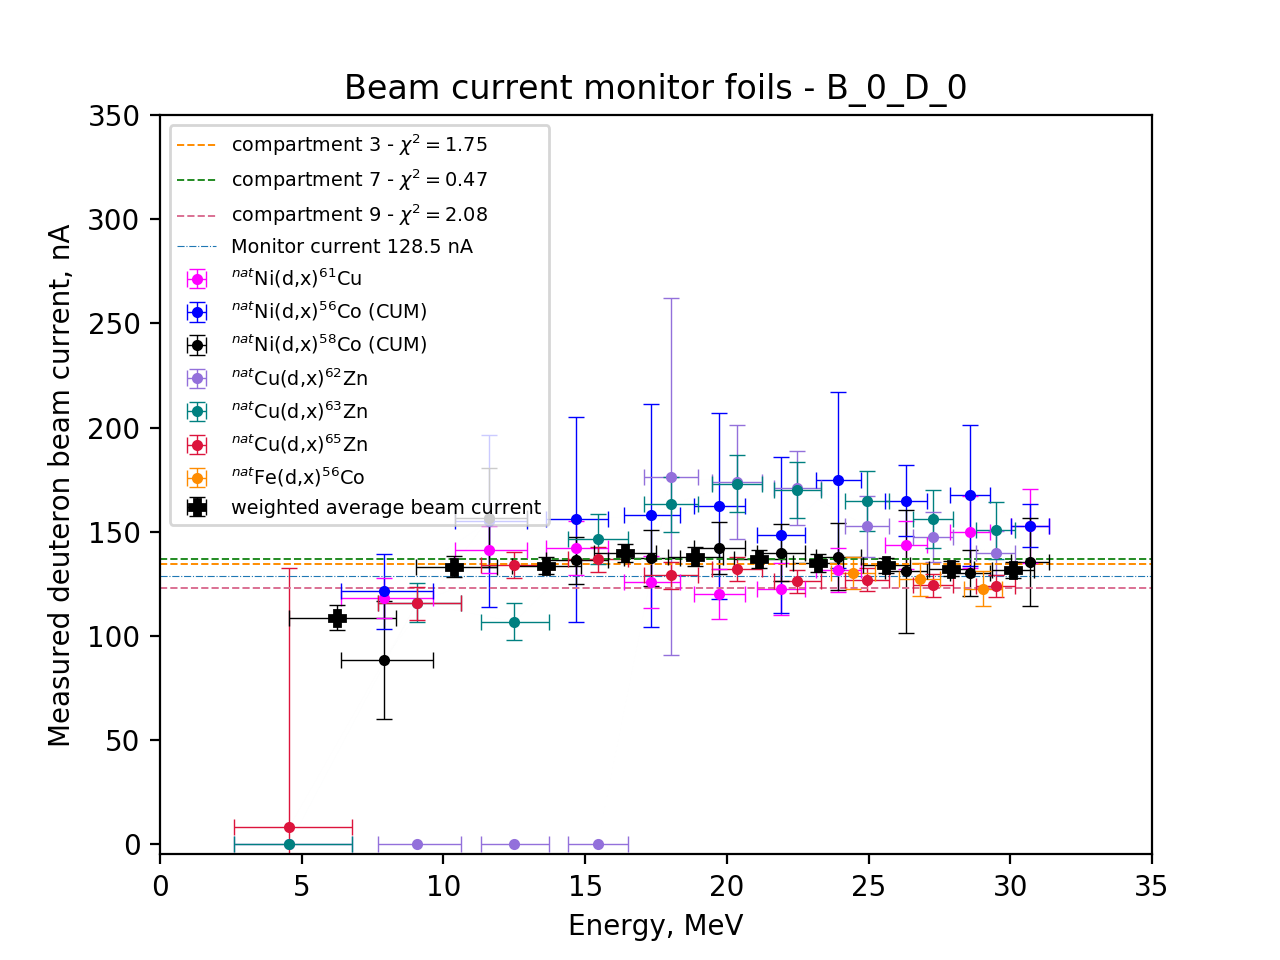
\includegraphics[width=8cm]{Analysis/B_0_D_0.png}
    %\subfloat[Before variance minimization]{{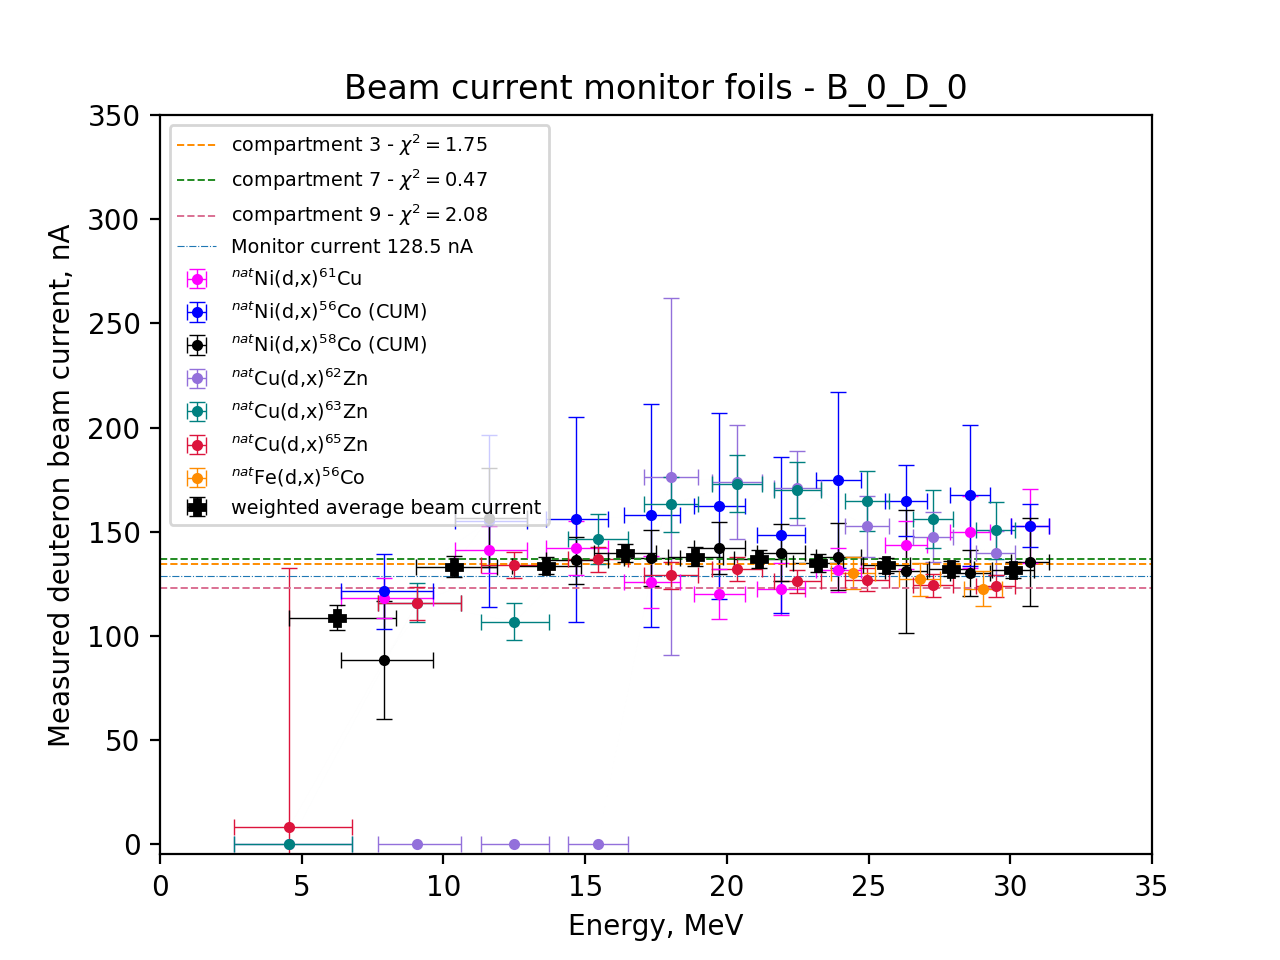
\includegraphics[width=8cm]{Analysis/B_0_D_0.png} }}%
%    \label{After variance minimization}
%    \end{subfigure}    
    %\subfloat[After variance minimization]{{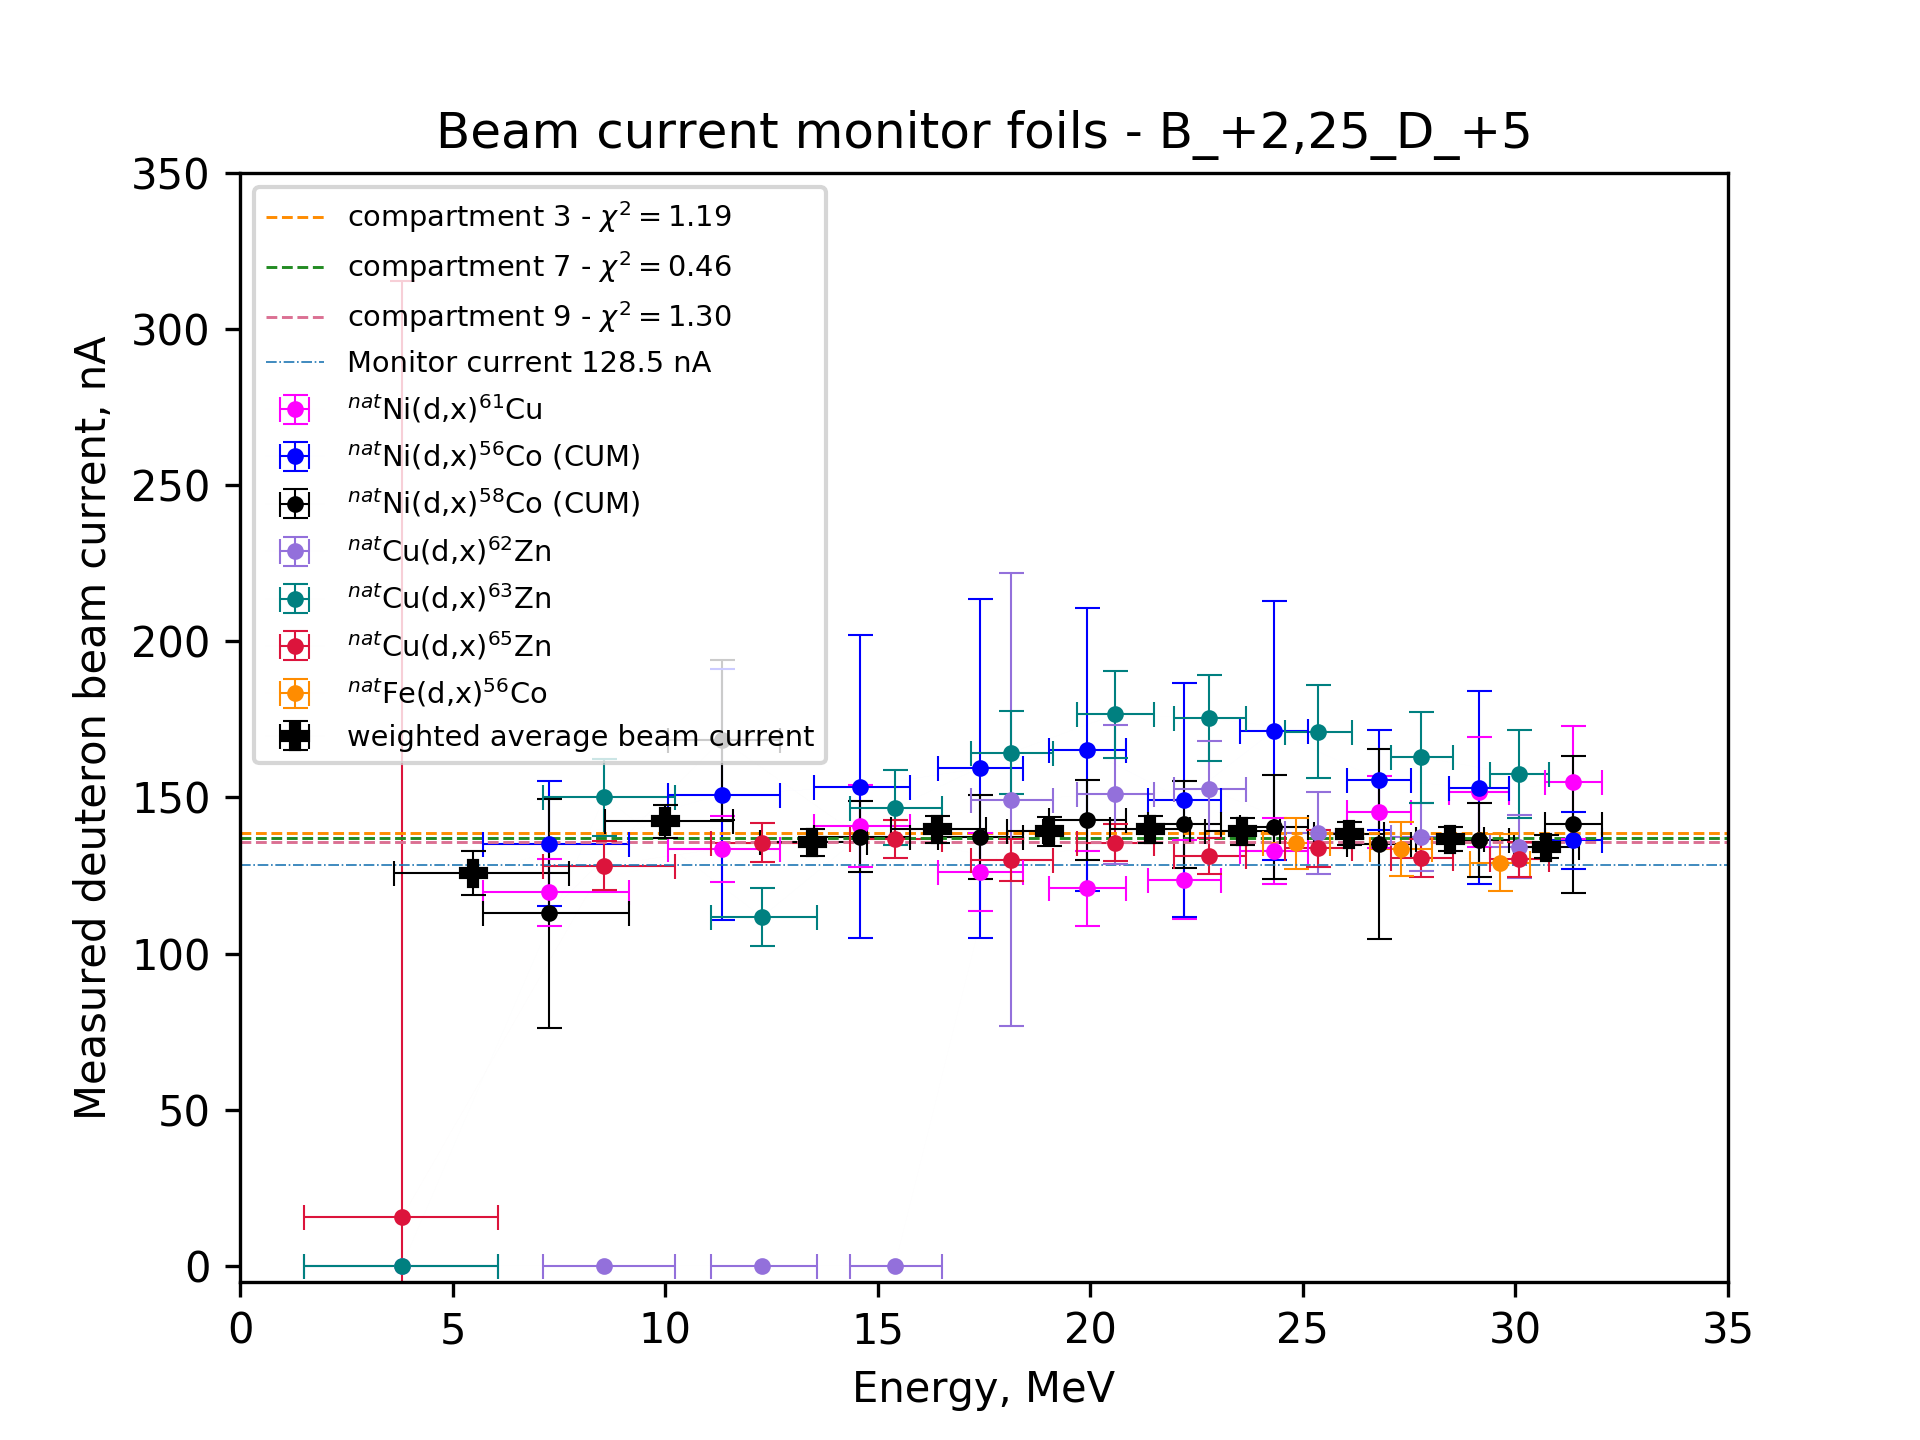
\includegraphics[width=8cm]{Analysis/comp_compared_B_+2,25_D_+5.png} }}%
    
%    \caption{Before, the current in the back of the stack is tending to be lower. The $\chi^2$ in the different compartments also tend to be higher. After variance minimization, the values for $\chi^2$ are smaller and the estimated current in each compartment agrees more with each other. We do not expect much of current degradation.}%
 %   \label{fig:varmin_beamcurrent}%
%\end{figure}


\subsubsection{The weighted averaged beam current, along with uncertainties}

Need to write statistical part first, about covariance matrix. 


Testing: the weighted average beam current for each target foil was used, to estimate the cross section. 

\begin{figure}%
    \centering    \subfloat{{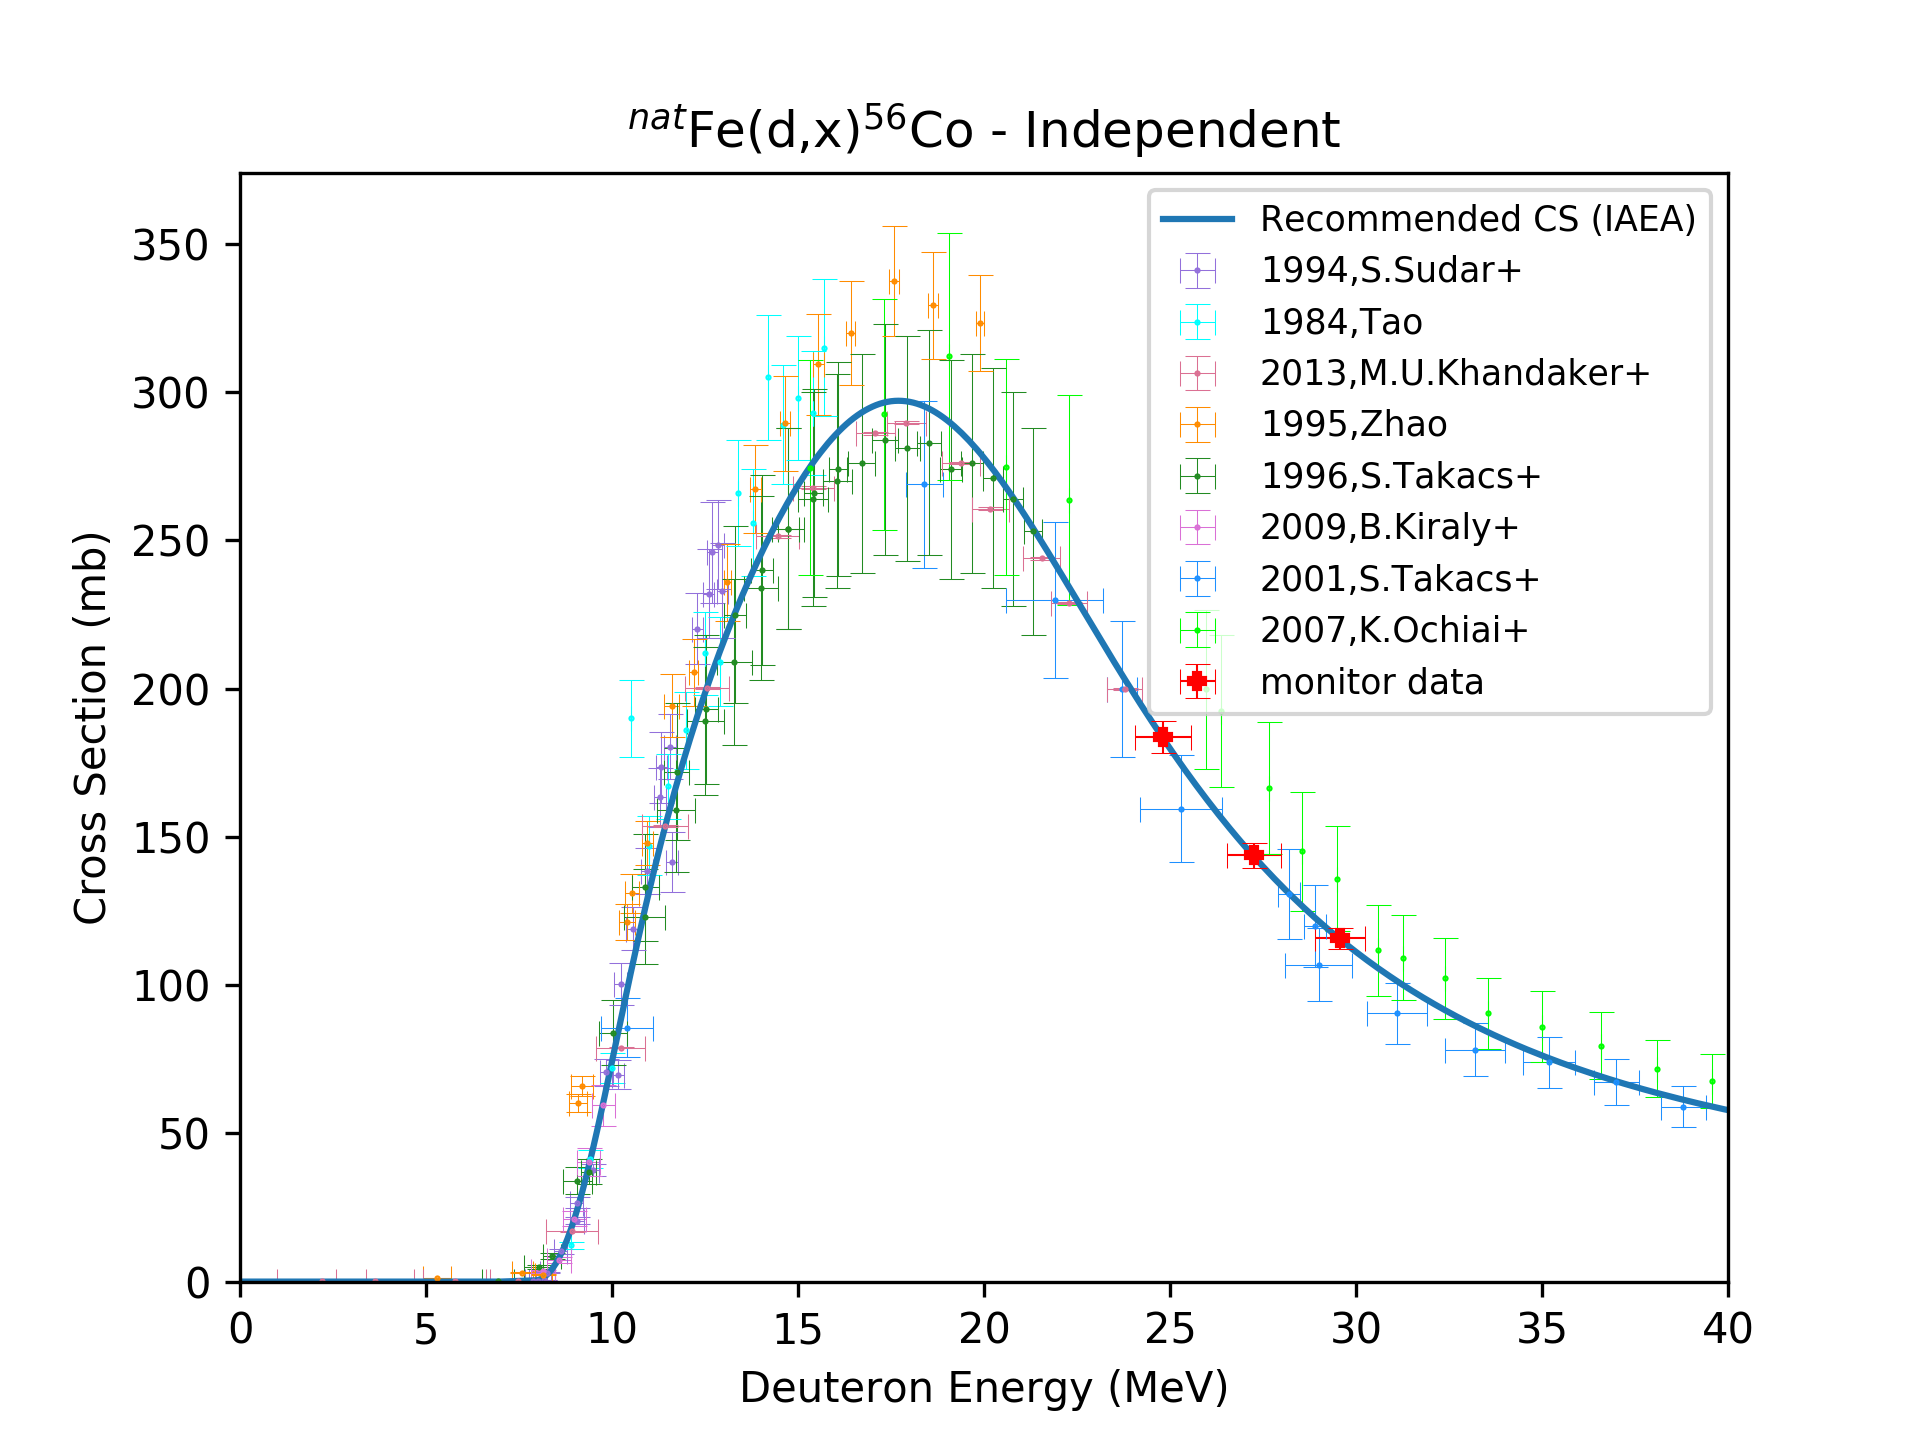
\includegraphics[width=8cm]{Results/Fe_56Co.png} }}%
    %\subcaption{....}
    \quad
    \subfloat{{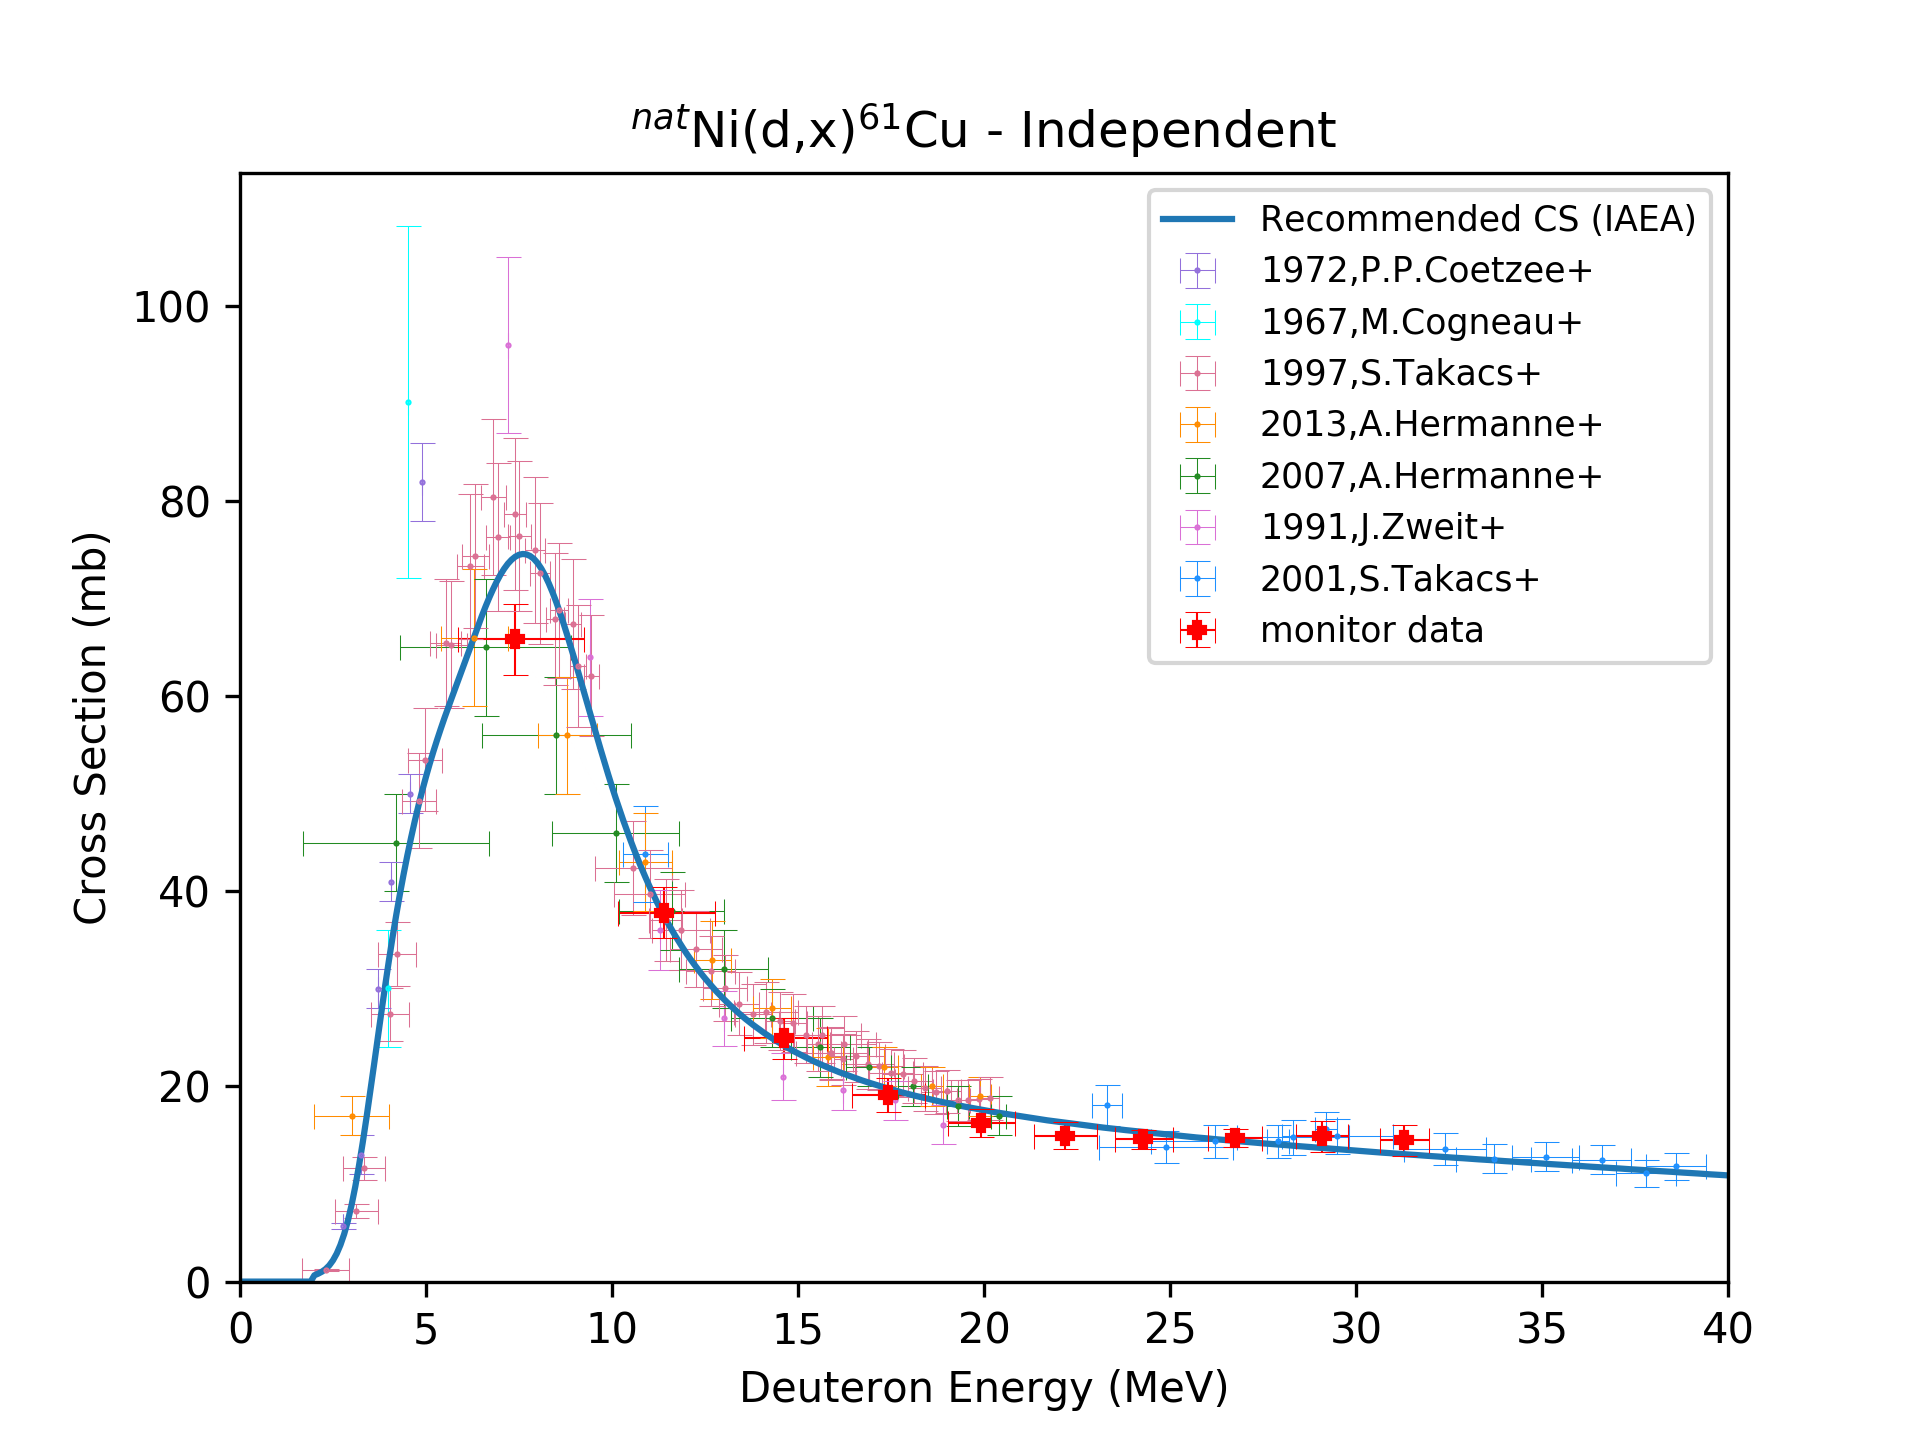
\includegraphics[width=8cm]{Results/Ni_61Cu.png} }}%
    \subfloat{{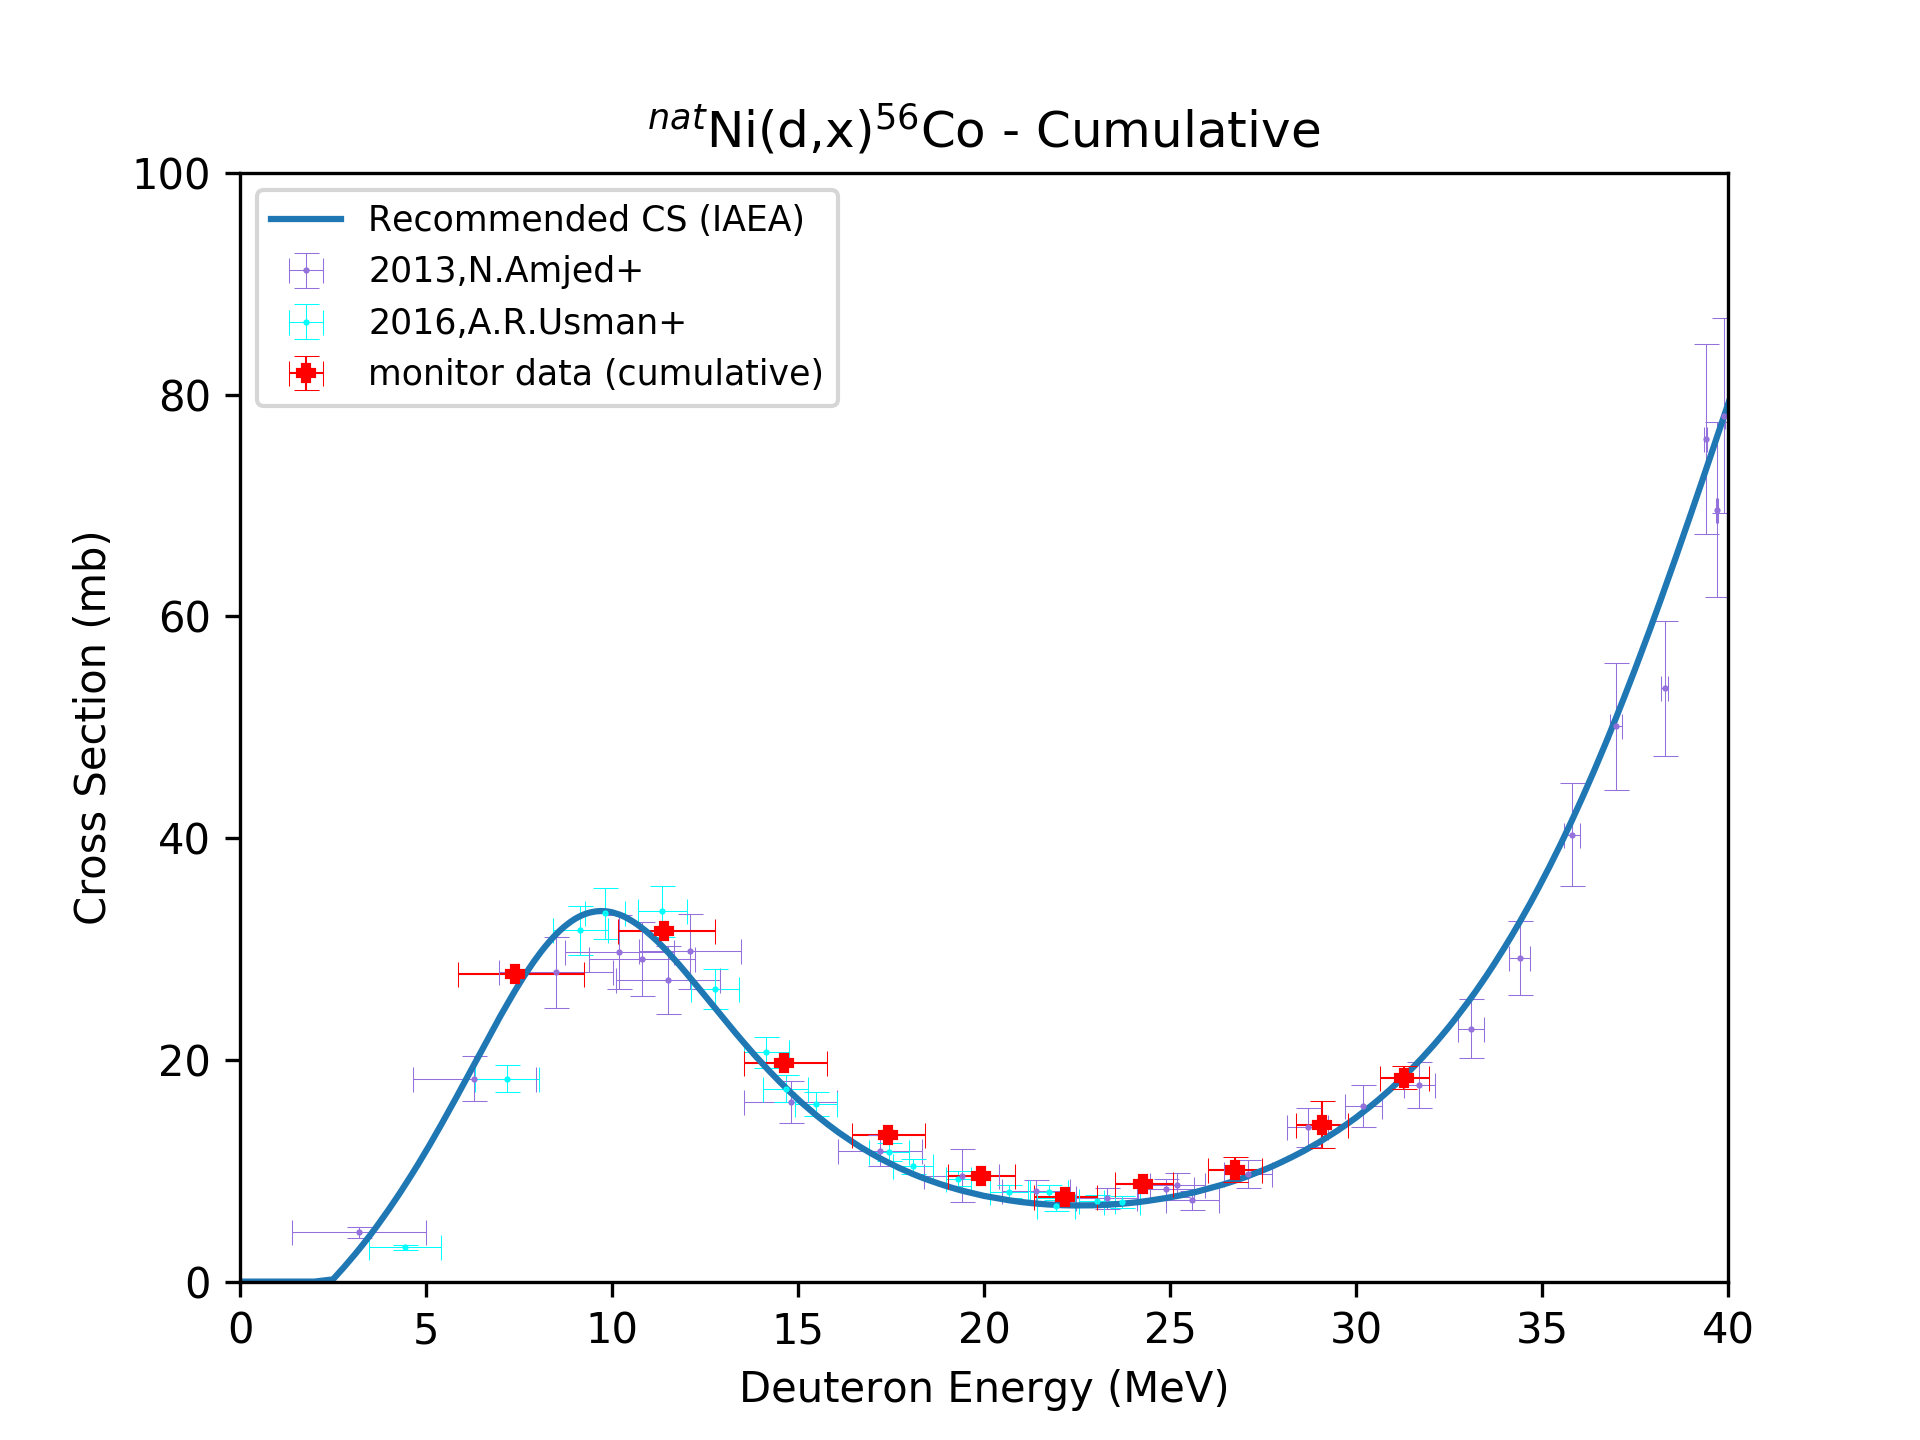
\includegraphics[width=8cm]{Results/Ni_56Co.png} }}%
    \quad
    \subfloat{{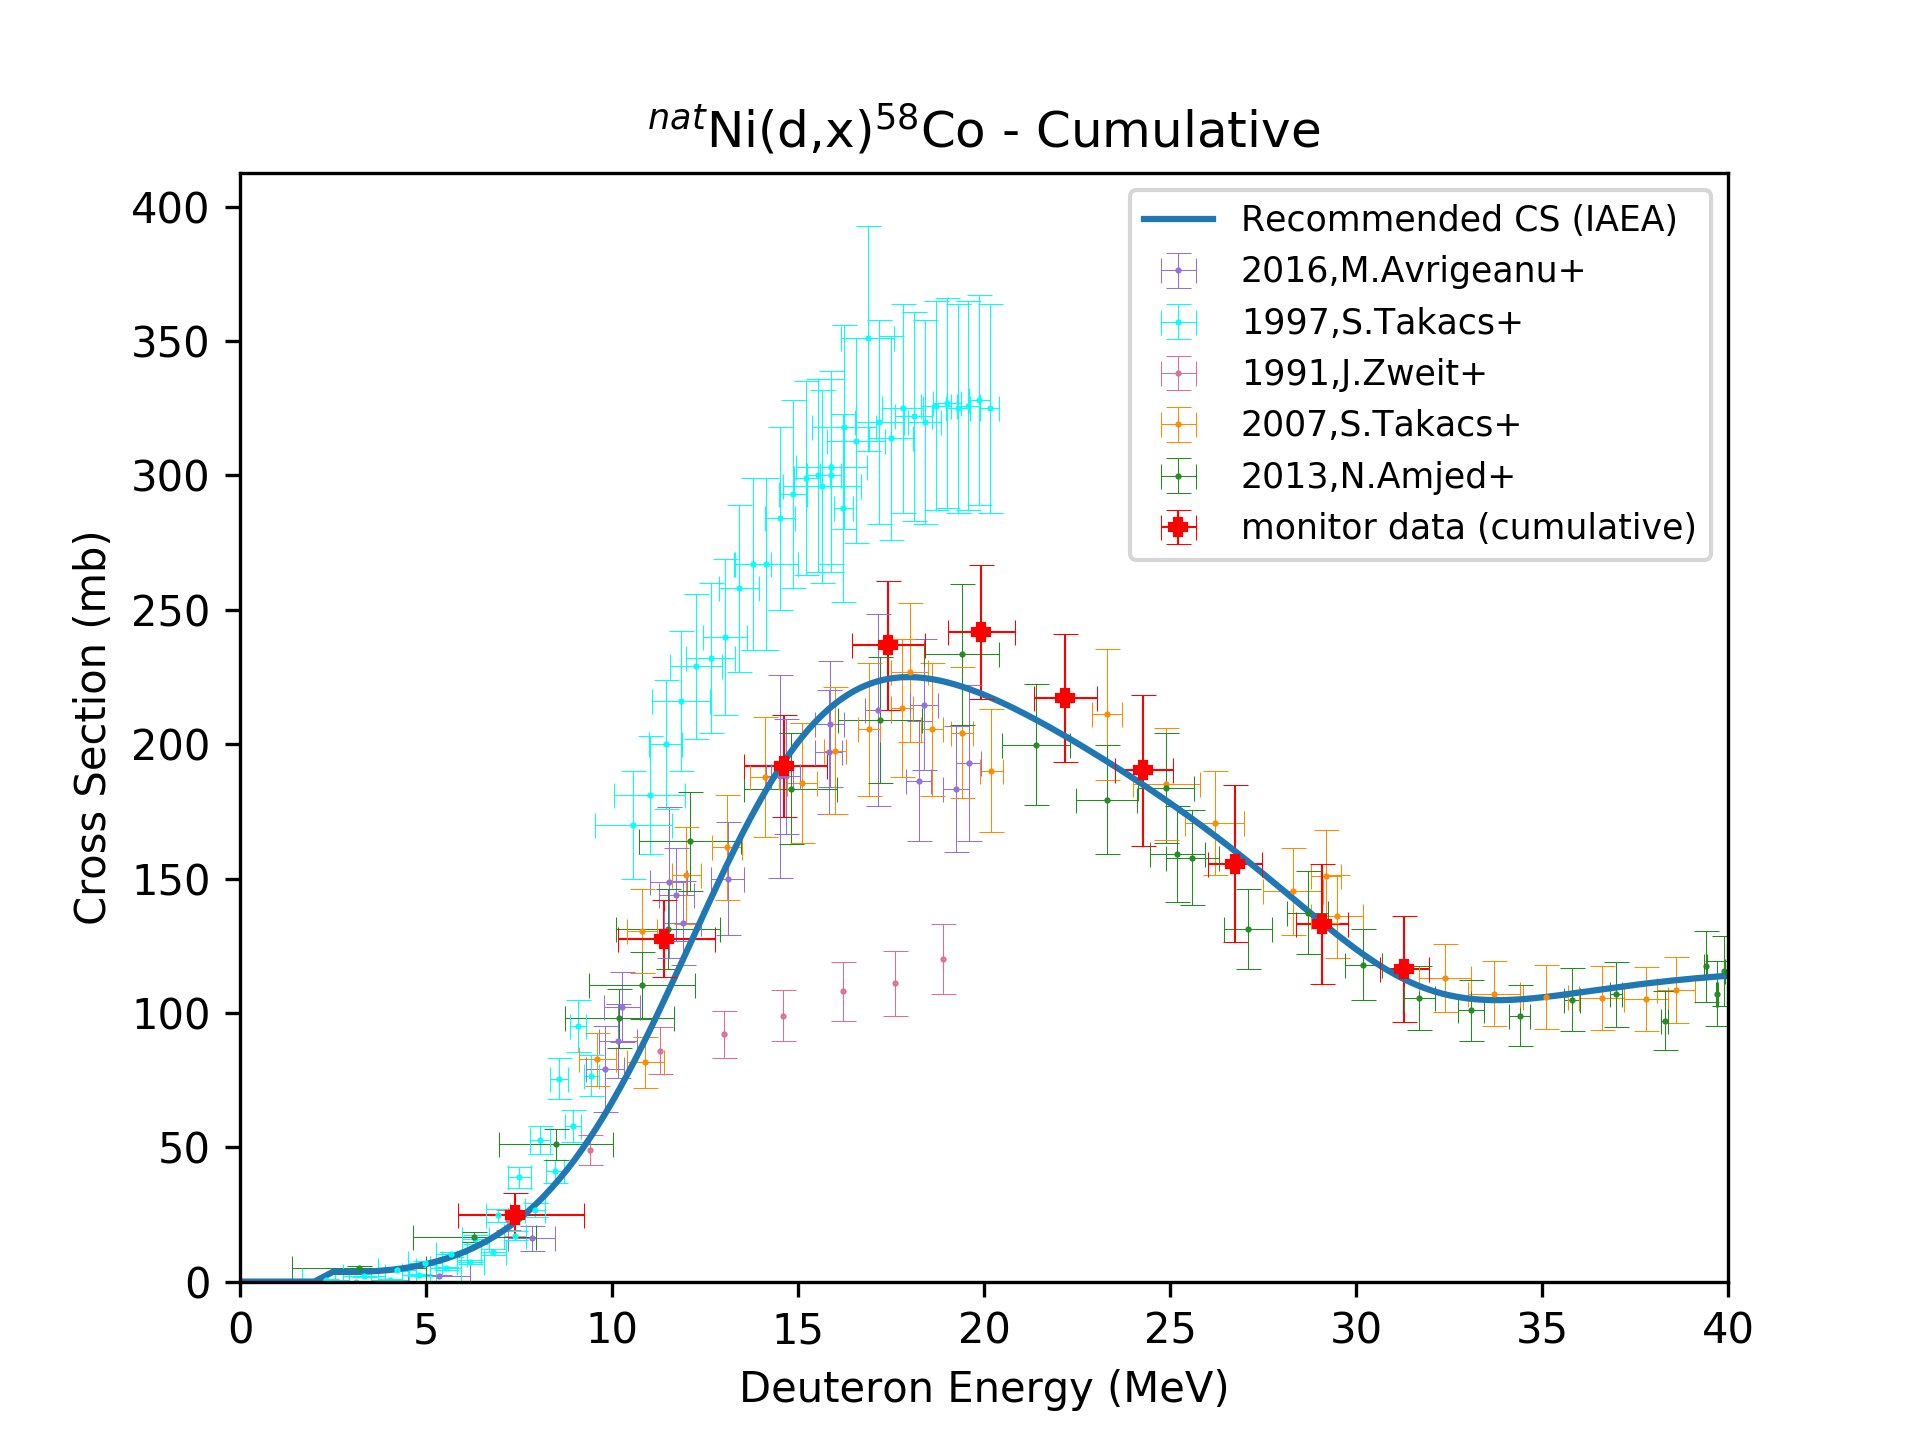
\includegraphics[width=8cm]{Results/Ni_58Co.png} }}%
    \quad
    \subfloat{{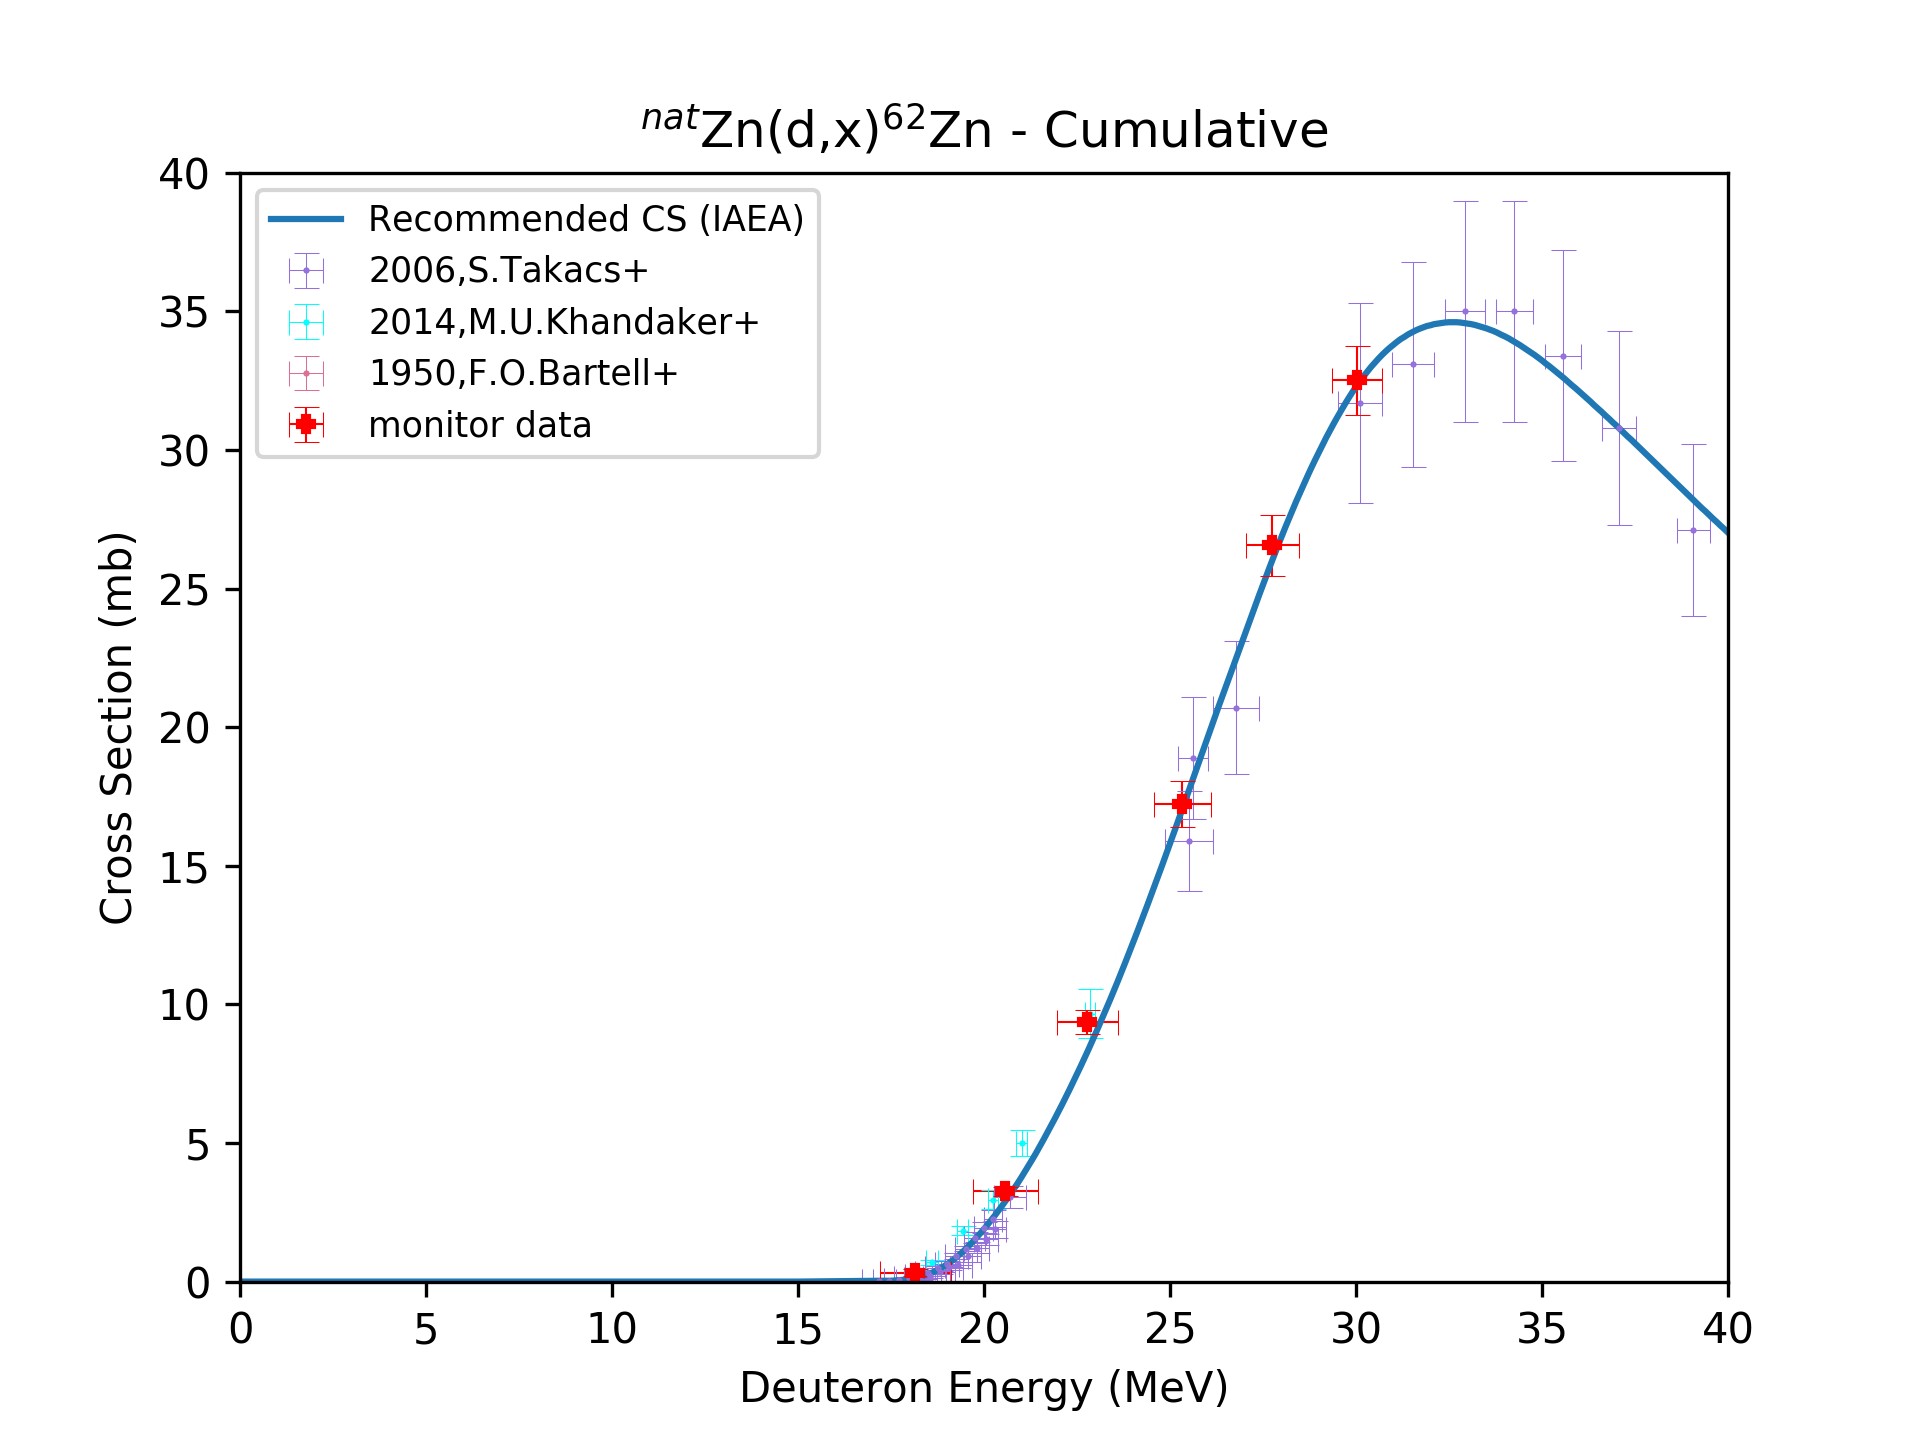
\includegraphics[width=8cm]{Results/Cu_62Zn.png} }}%
    \quad
    \subfloat{{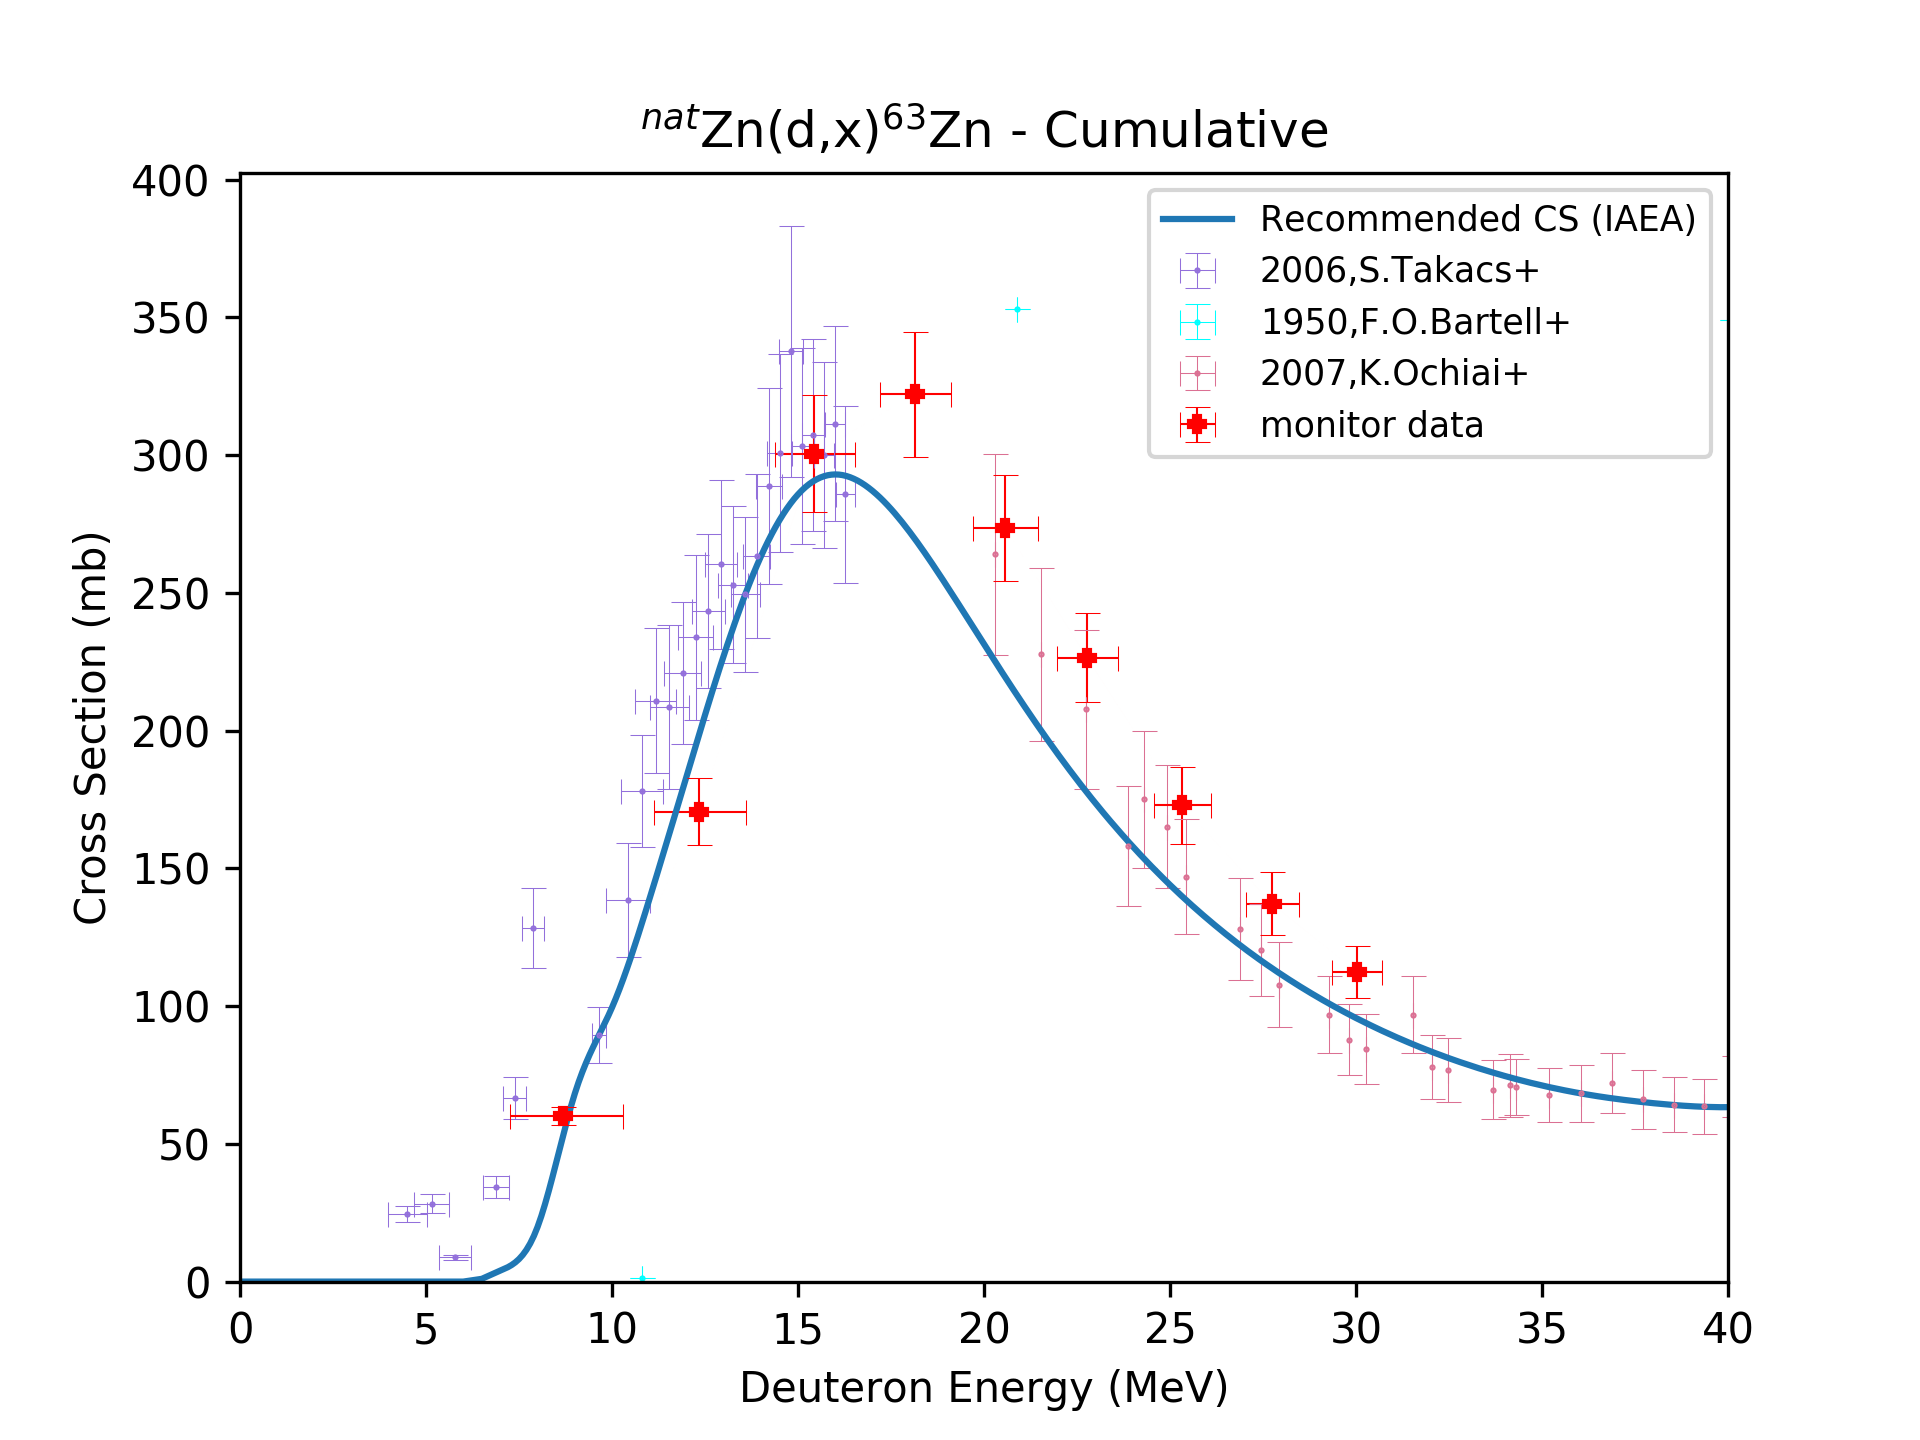
\includegraphics[width=8cm]{Results/Cu_63Zn.png} }}%
    \quad
    \subfloat{{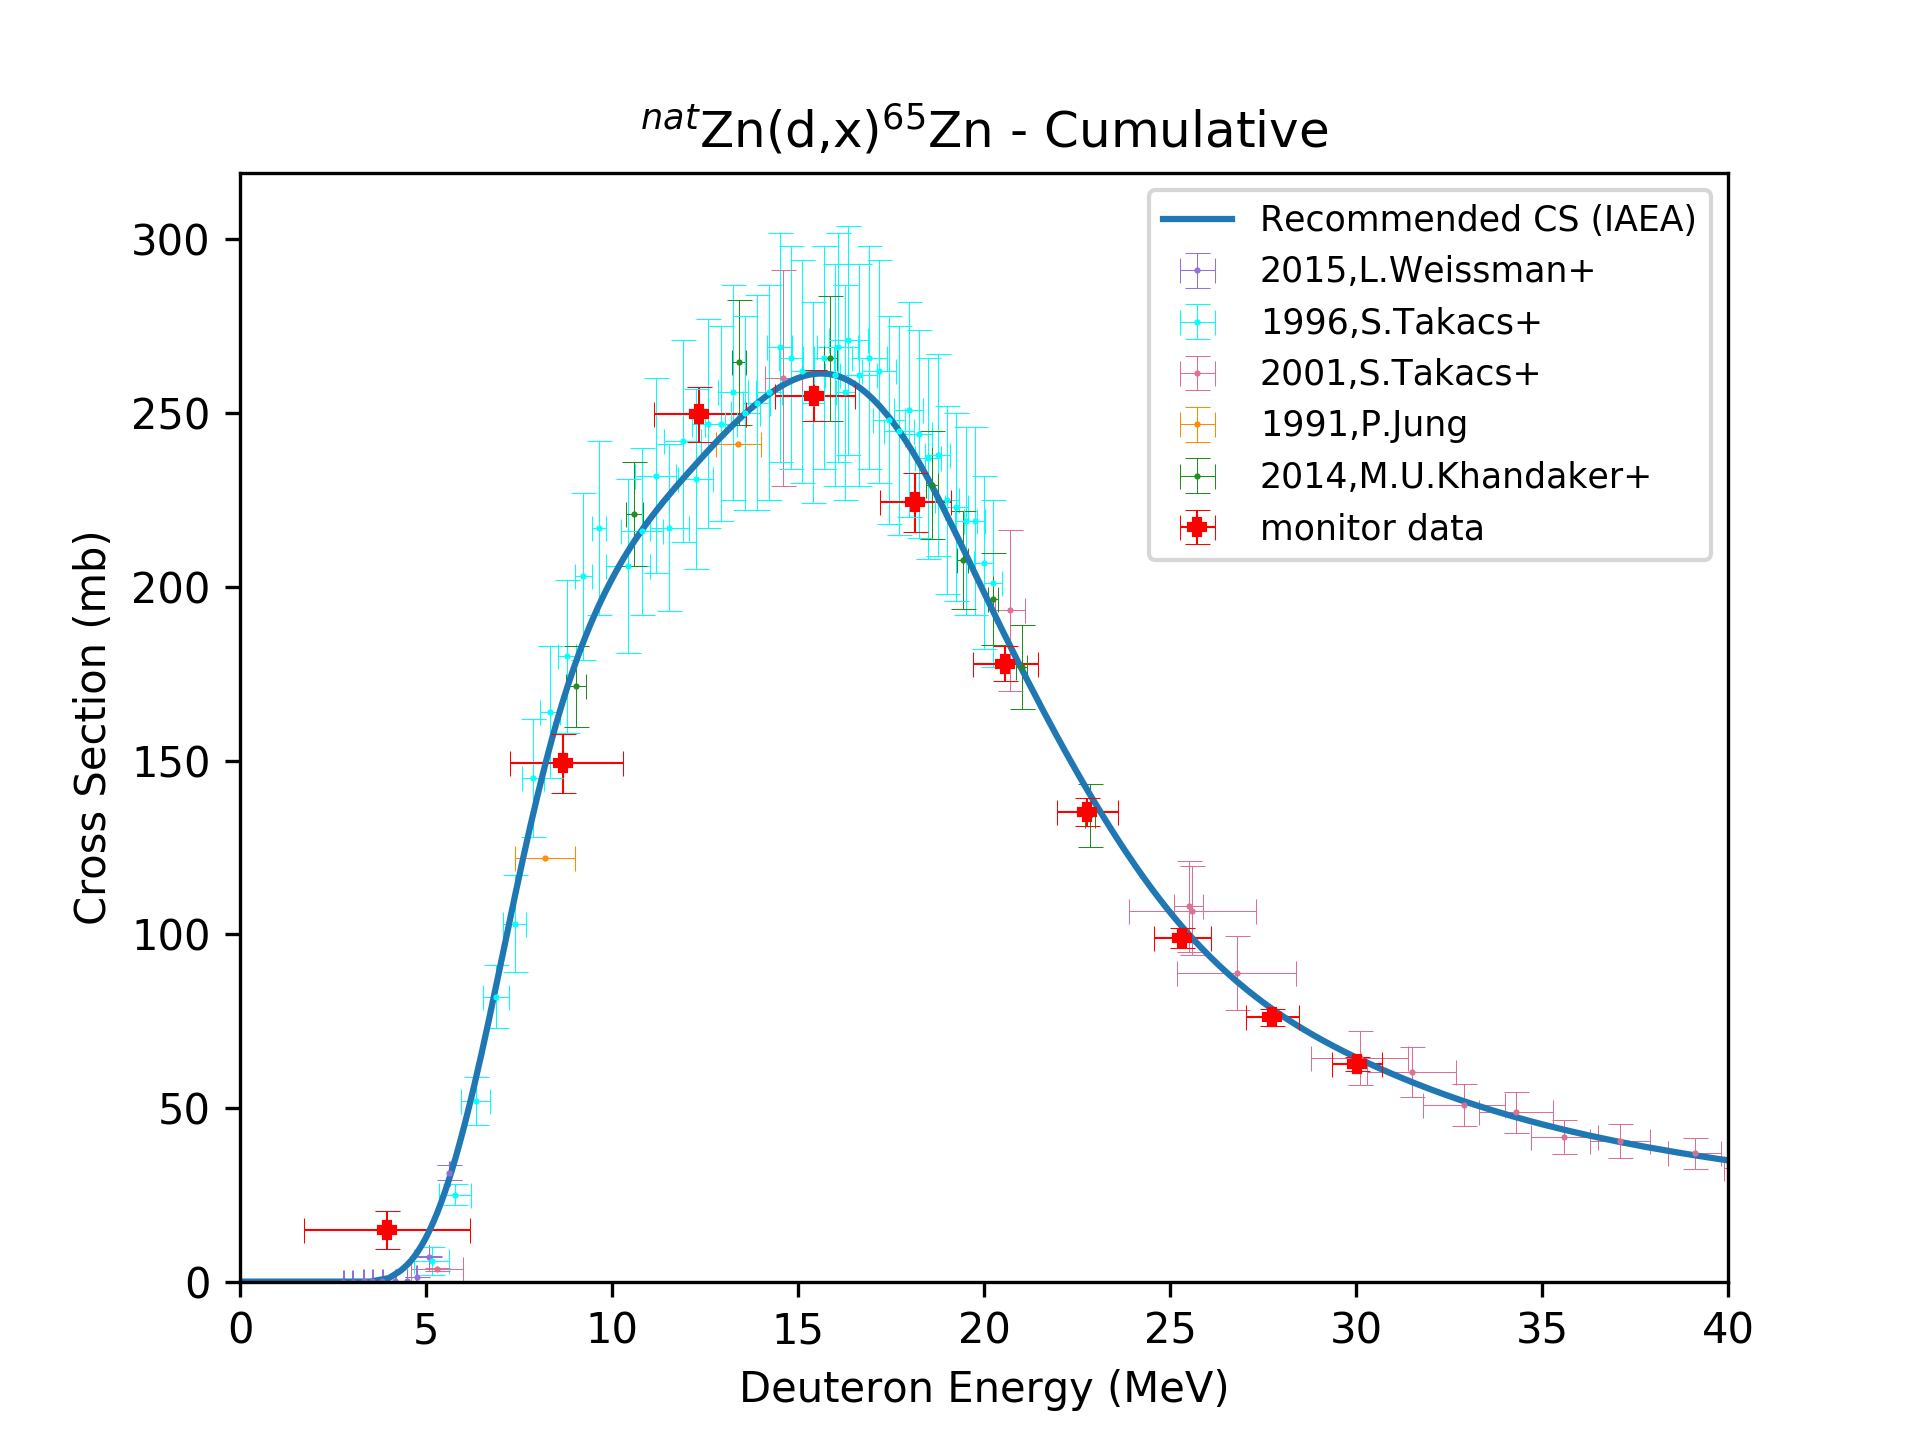
\includegraphics[width=8cm]{Results/Cu_65Zn.png} }}%
    \quad
    \caption{Figure shows the estimation of monitor cross section using the calculated beam current. It is compared along with the monitor data.  }%
    \label{fig:monitor_BC}%
\end{figure}



\subsection{Production Cross sections}

Once the weighted average beam current was estimated, the cross sections were estimated using equation \ref{eq:CS_ch3}. For decay chains, the first observed element was reported as cumulative, unless it was the first entry. If there was independent measurements of the daughter products, they were reported as independent and cumulative along with the parent. \\

\subsubsection{Reaction modeling}
In addition to measurements and experimental data, different reaction modeling packages such as ALICE, TALYS, TENDL, COH and EMPIRE will be plotted. 

}

\chapter{Results}\label{Chapter:Results}
\noindent

\section{Iridium cross sections}

\begin{figure}%
    \centering
    \subfloat{{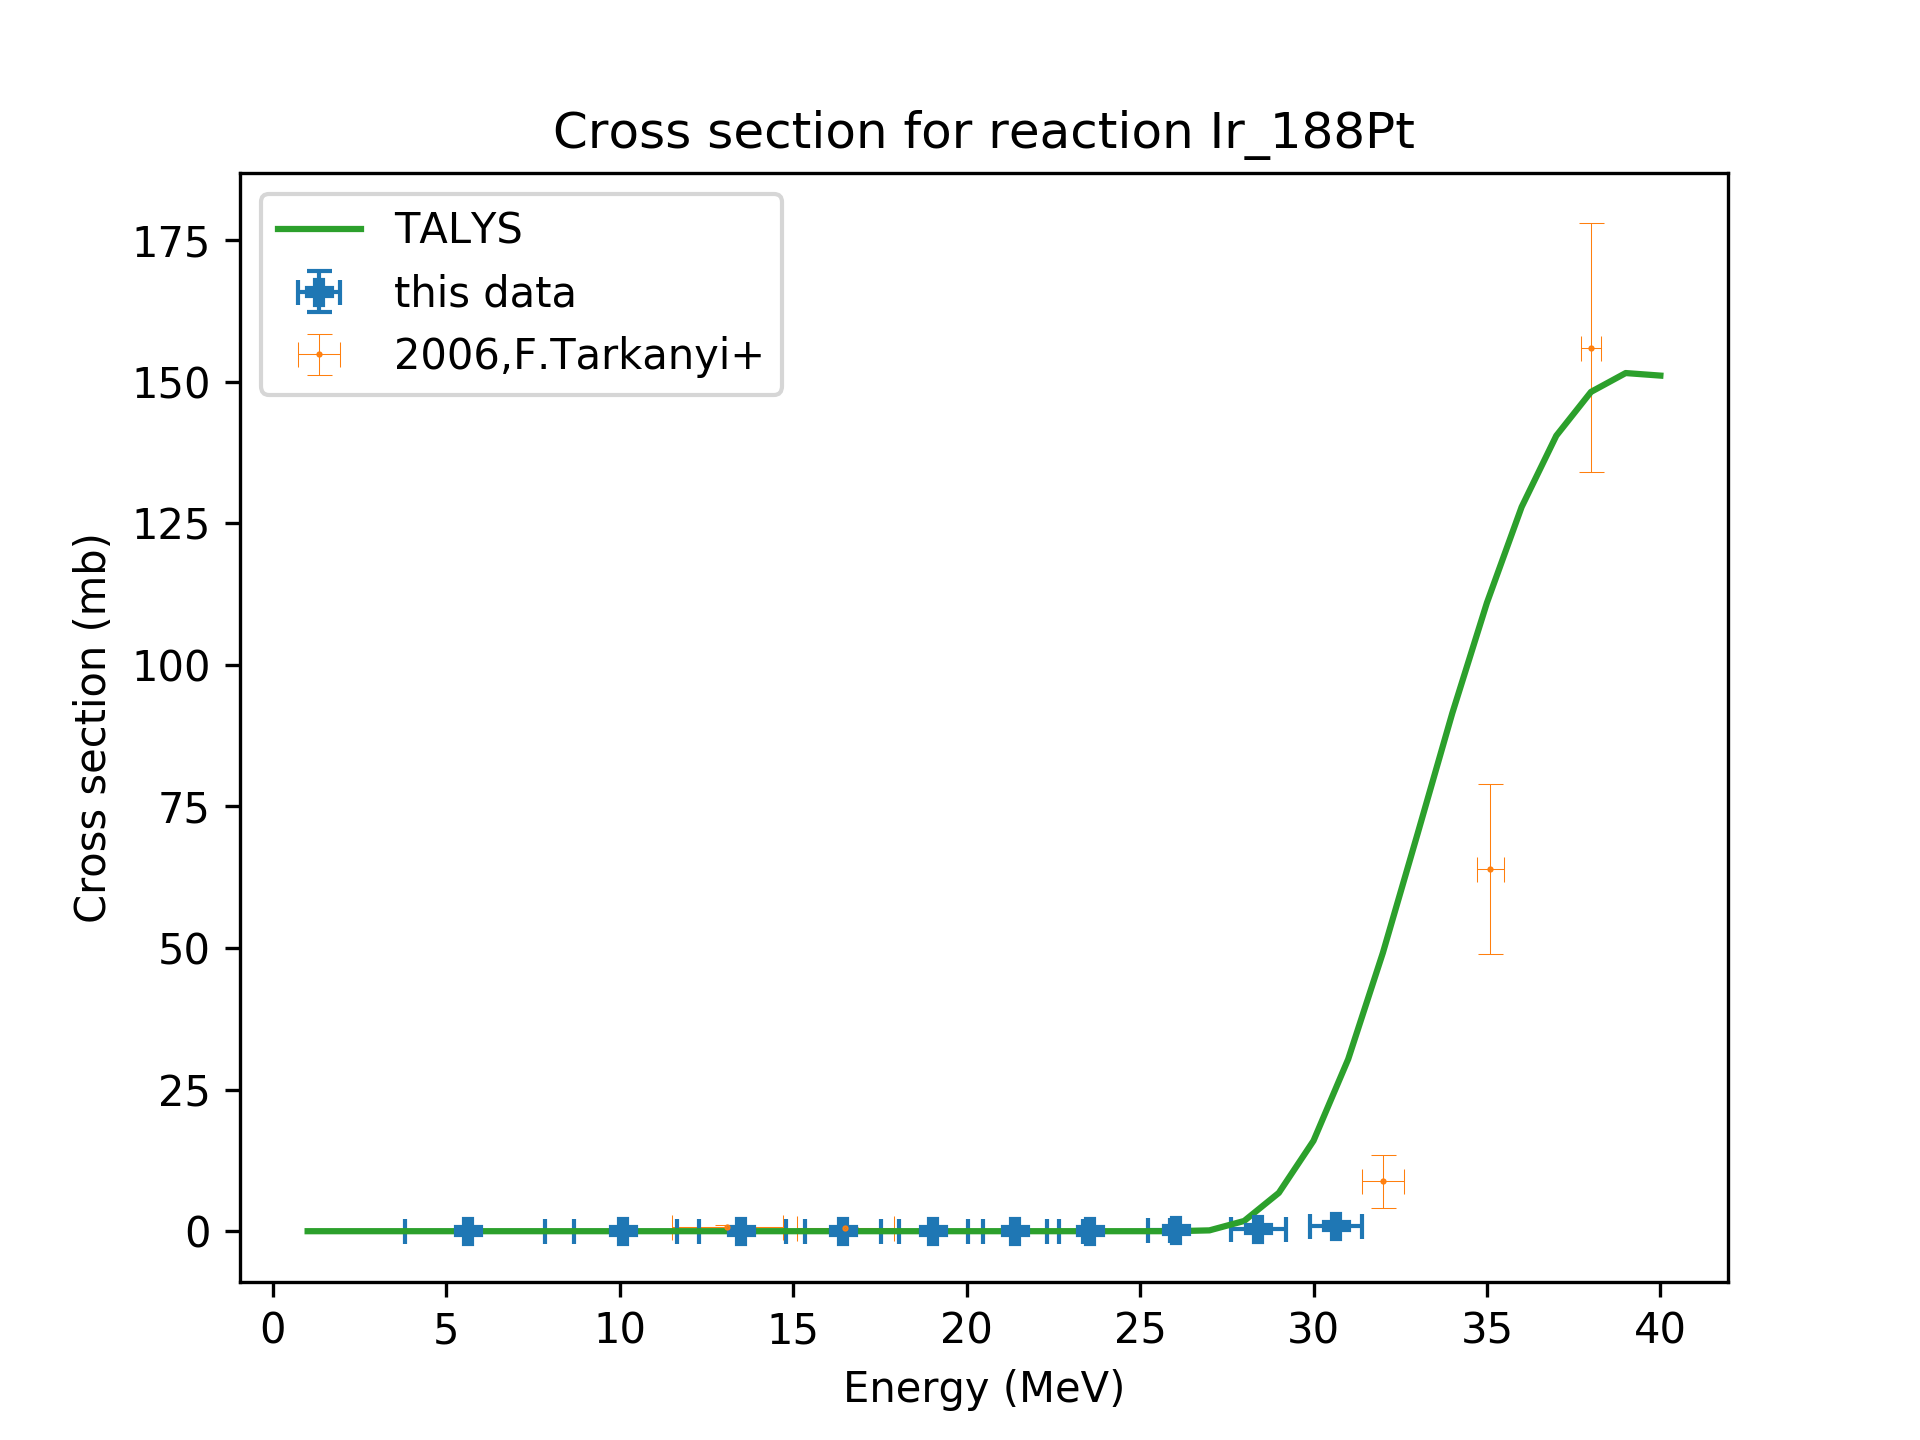
\includegraphics[width=7.5cm]{Results/Ir_188Pt.png}}%
    \subcaption{...}
    \label{subfig:188Pt_plot}
    \quad
    \subfloat{{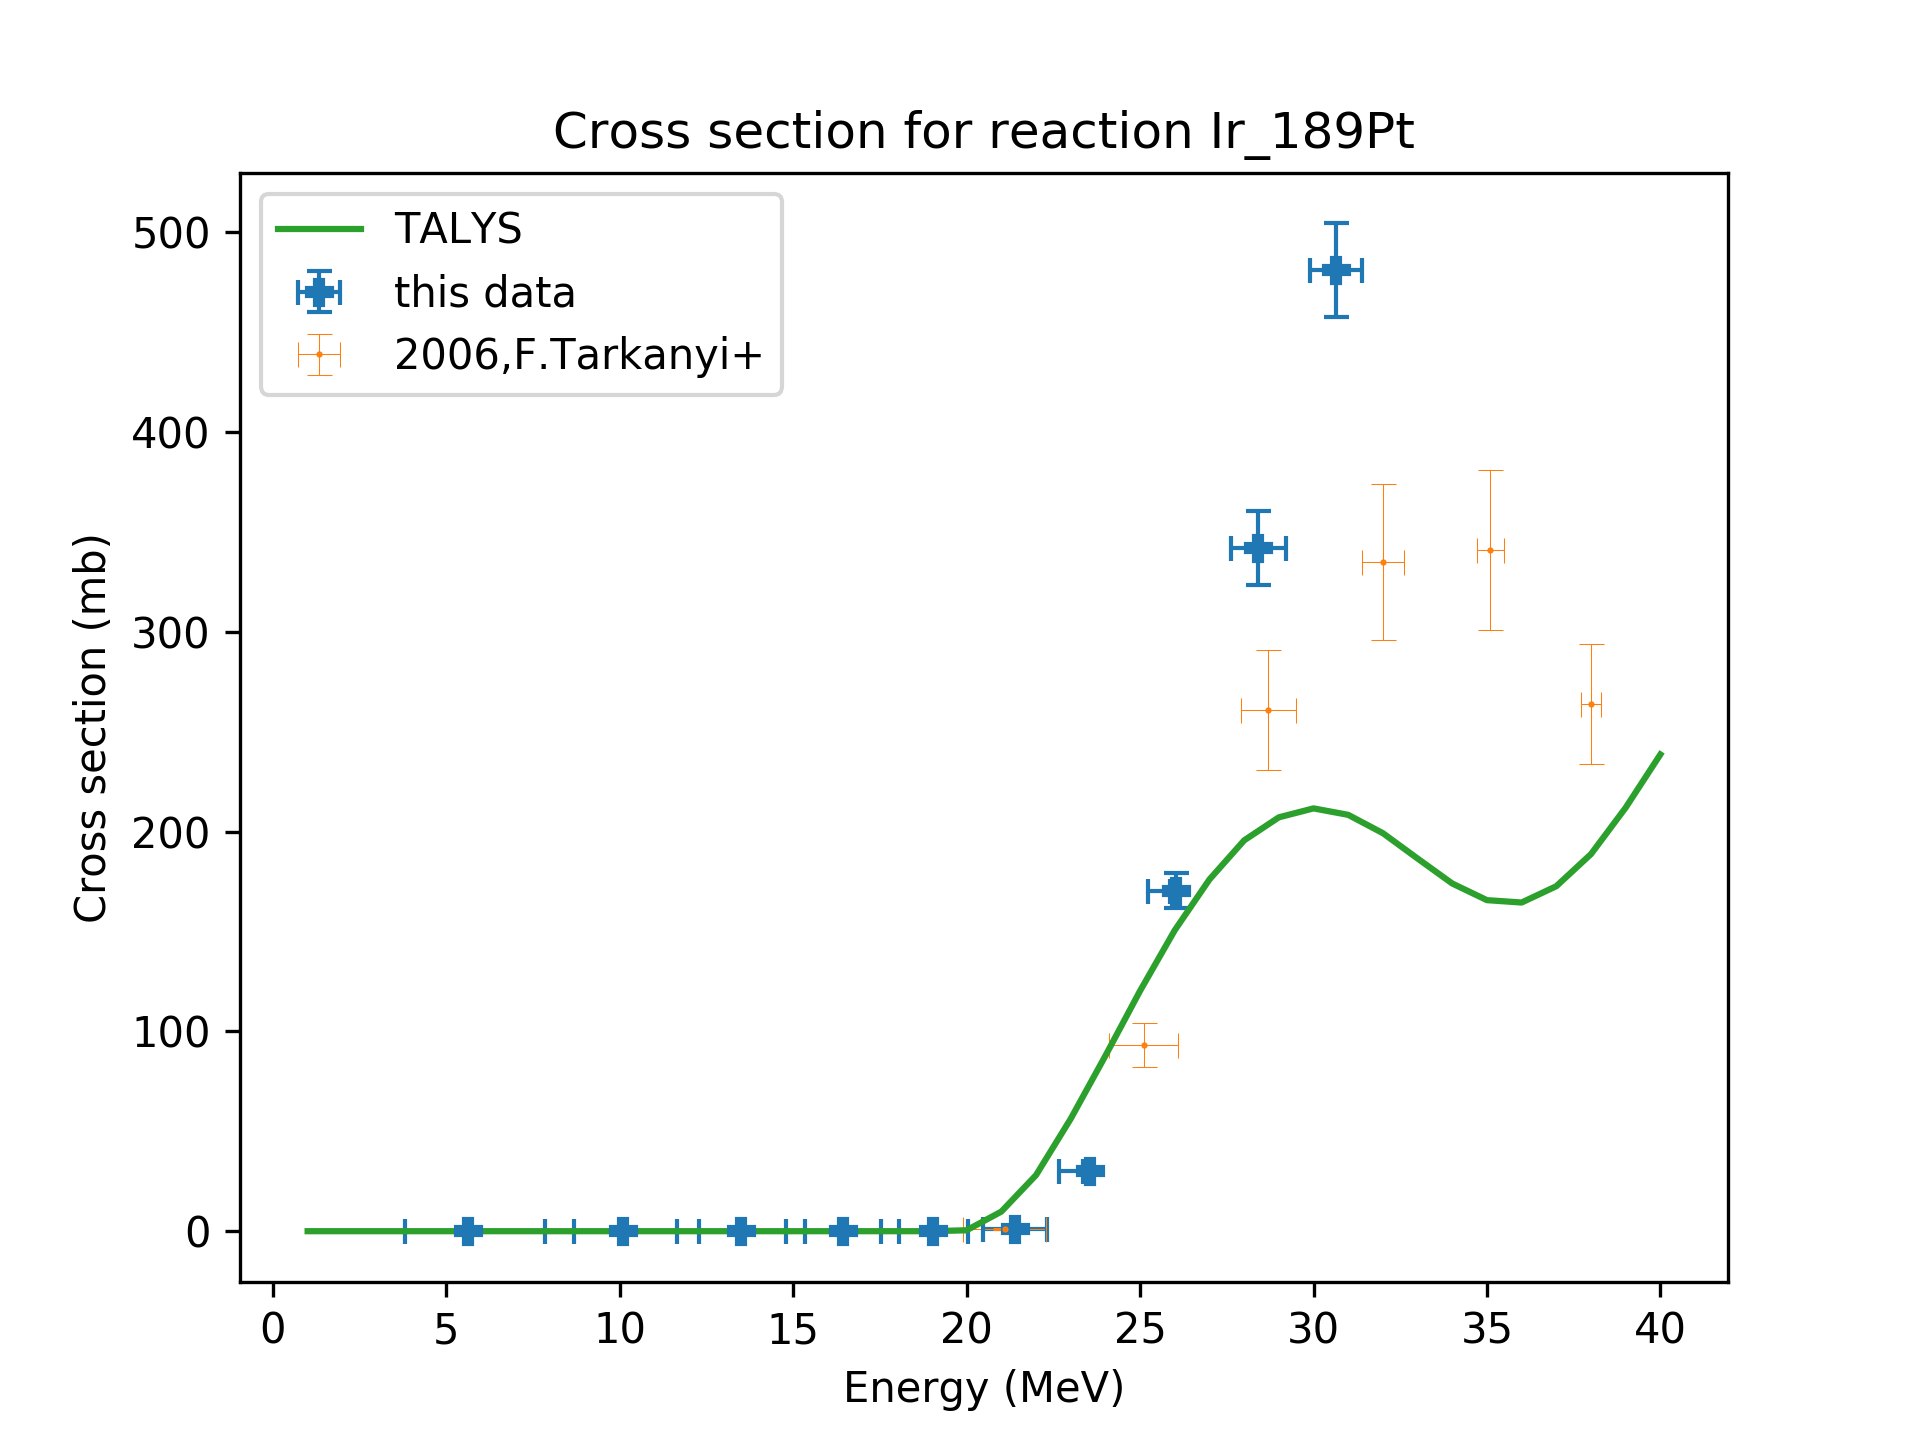
\includegraphics[width=7.5cm]{Results/Ir_189Pt.png} }}%
    \subcaption{...}
    \label{subfig:189Pt_plot}
    \subfloat{{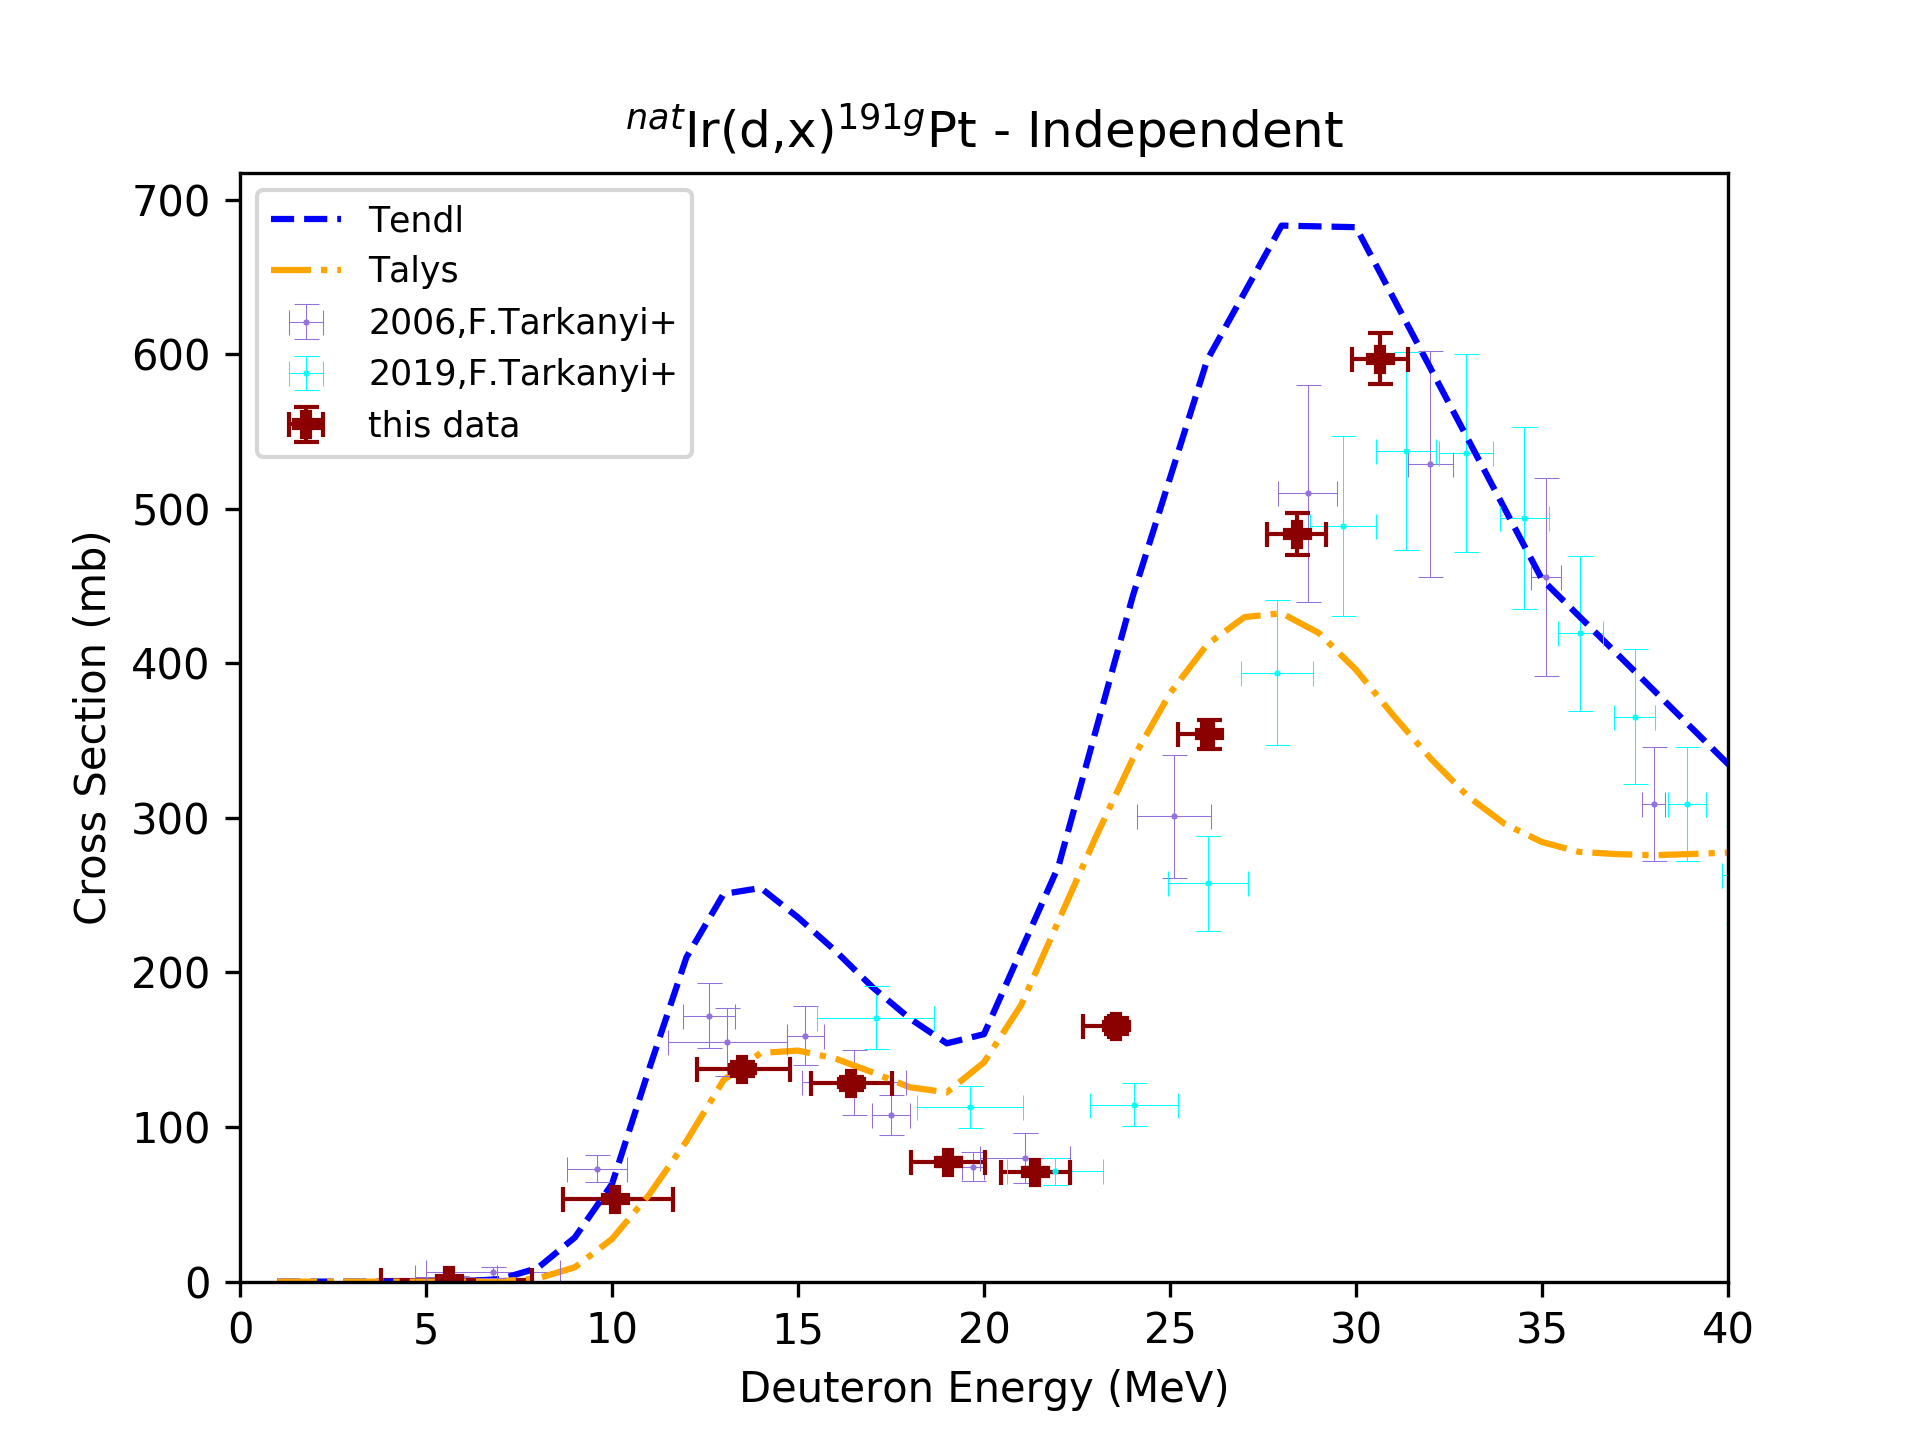
\includegraphics[width=7.5cm]{Results/Ir_191Pt.png} }}%
    \subcaption{...}
    \label{subfig:191Pt_plot}
    \quad
    \subfloat{{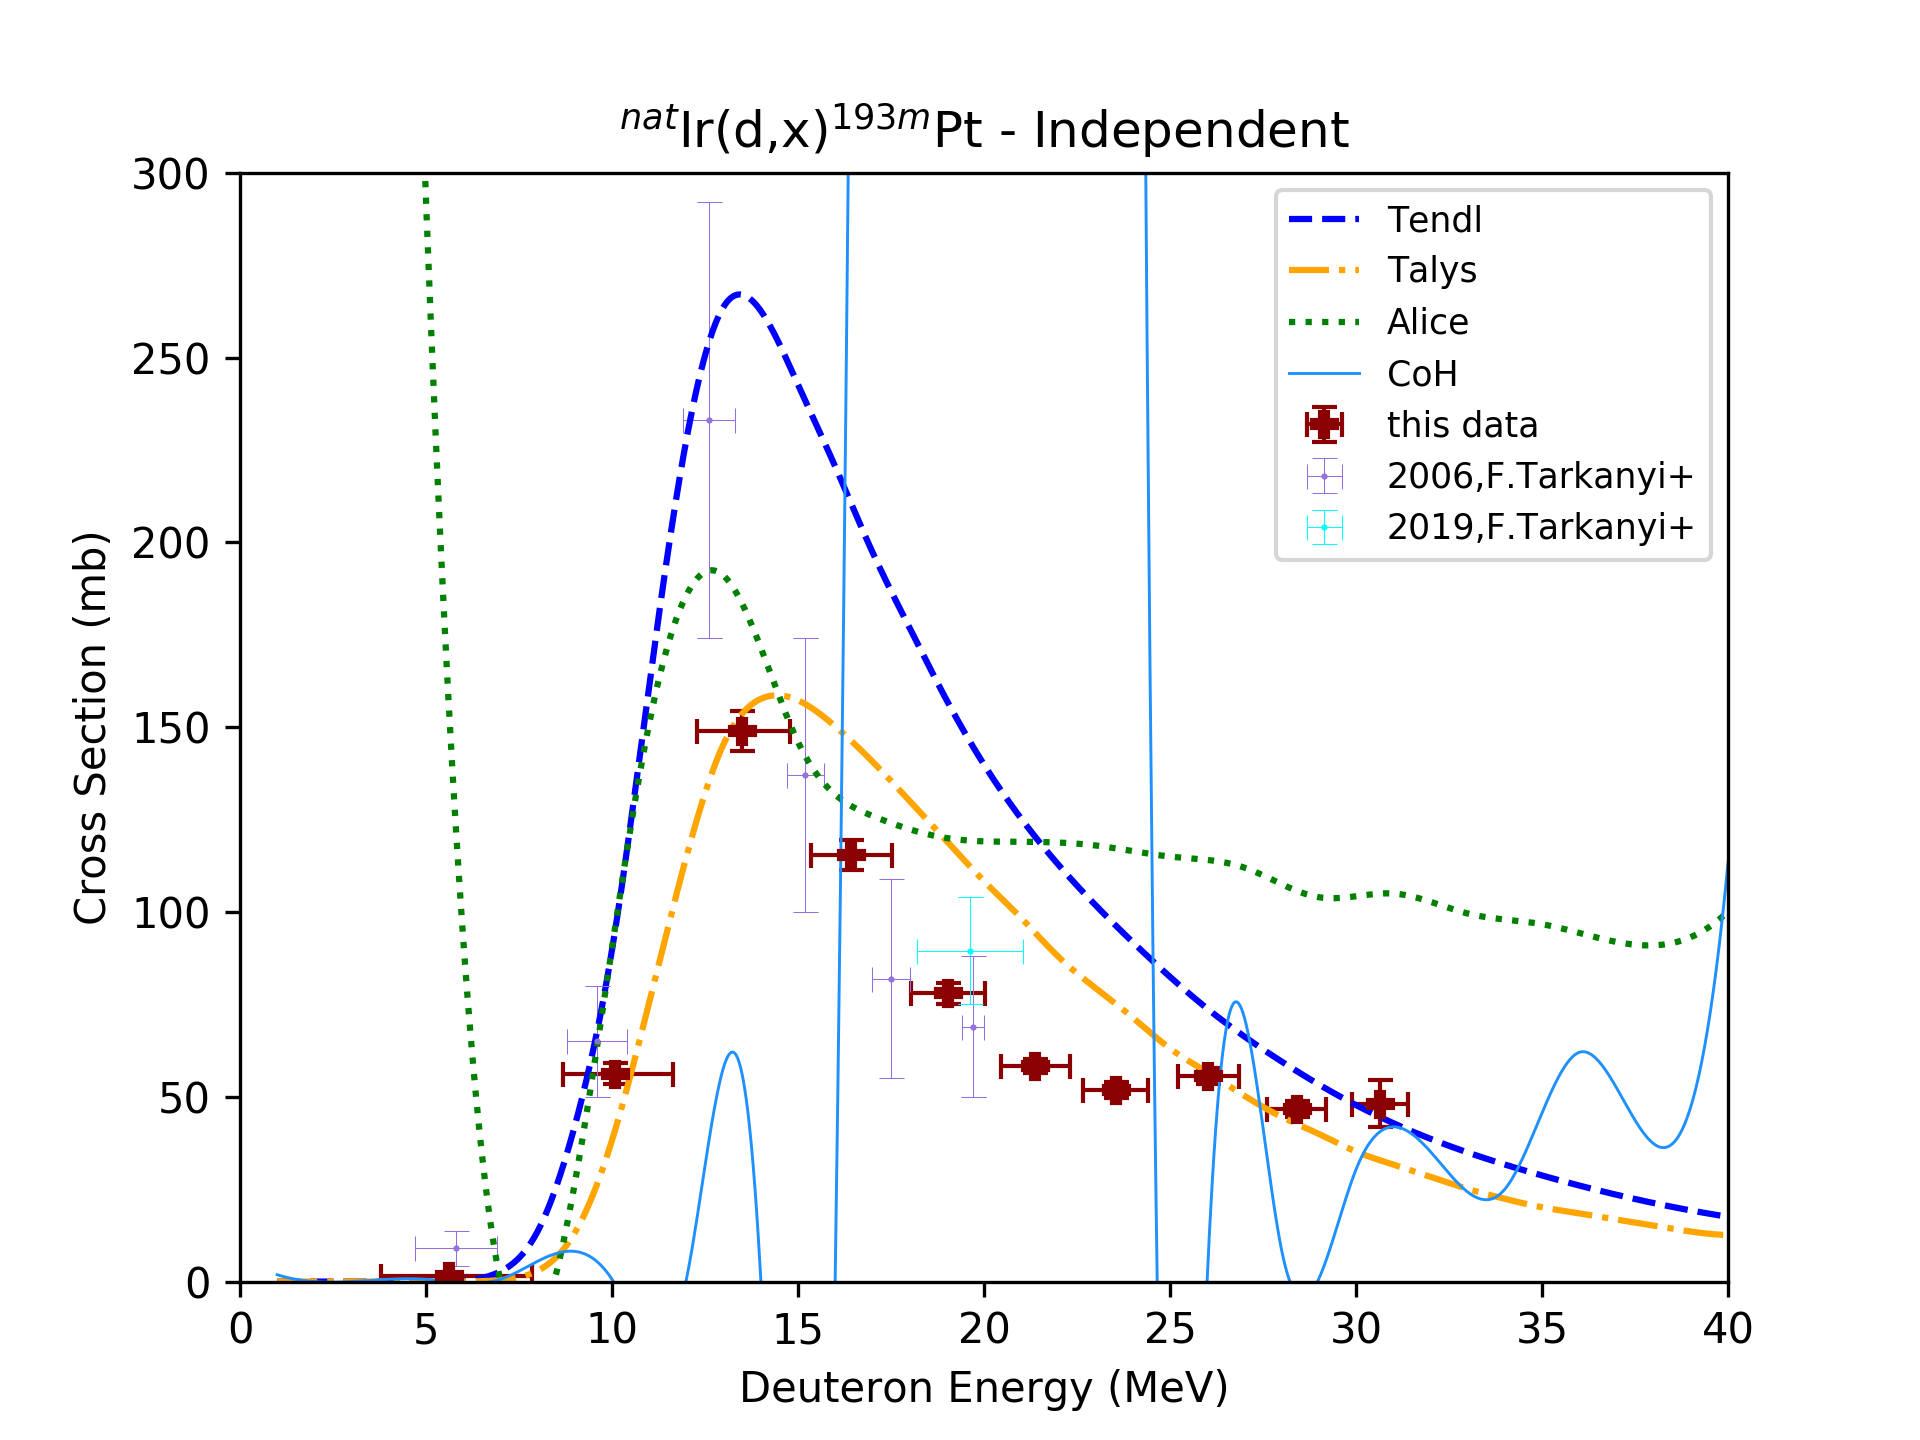
\includegraphics[width=7.5cm]{Results/Ir_193mPt.png} }}%
    \subcaption{...}
    \label{subfig:193mPt_plot}
    \caption{Cross section plots for Pt-product nuclei.  }%
    \label{fig:Pt_CrossSections}%
\end{figure}


\begin{figure}%
    \centering
    \subfloat{{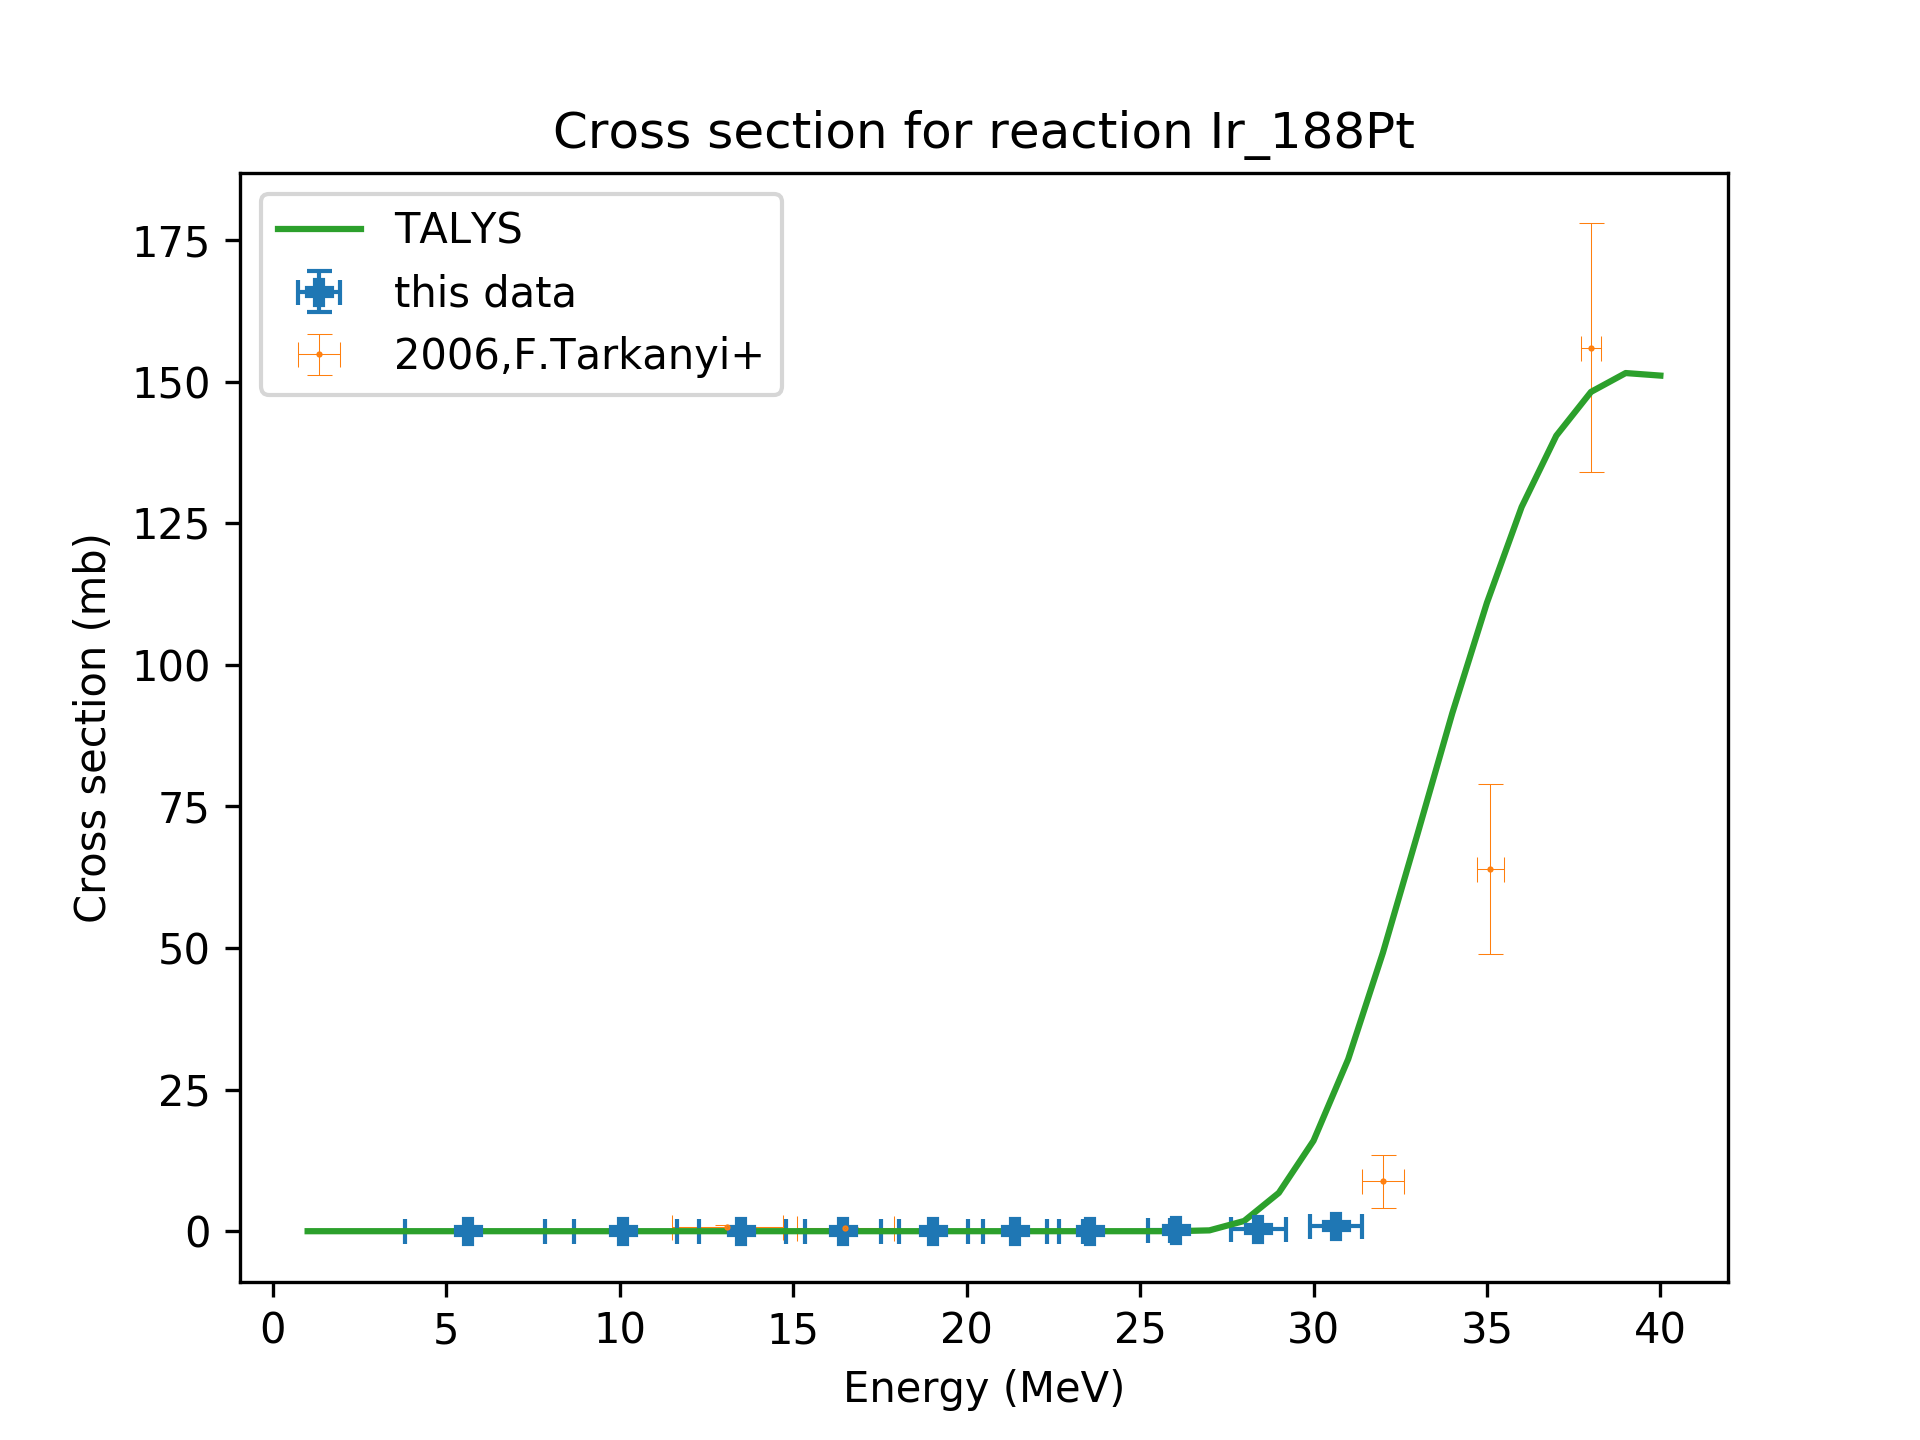
\includegraphics[width=5cm]{Results/Ir_188Pt.png}}%
    \quad
    \subfloat[]{{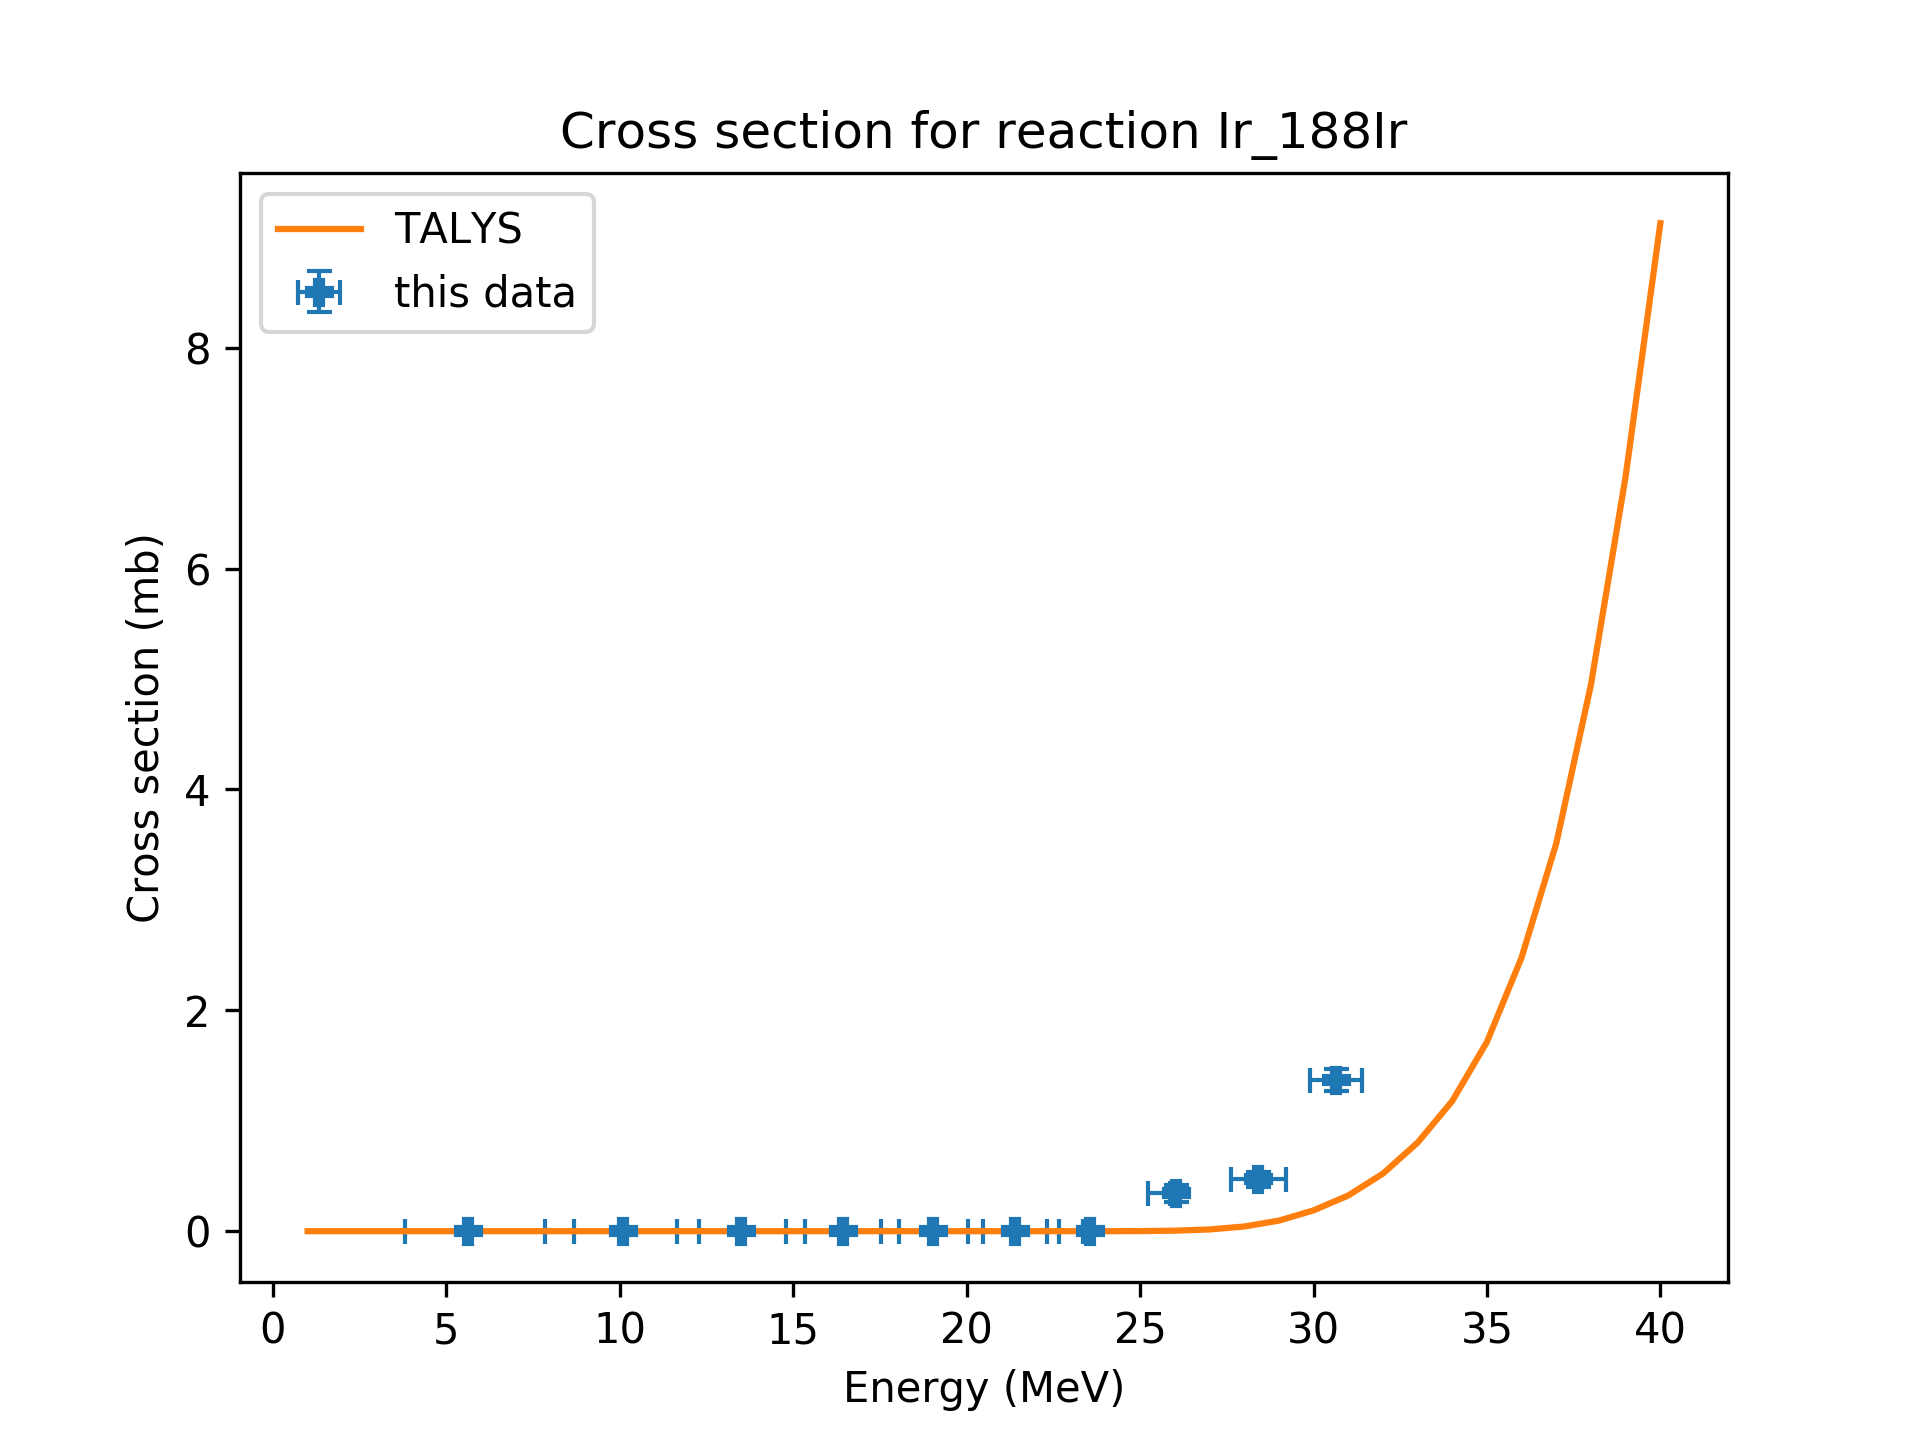
\includegraphics[width=5cm]{Results/Ir_188Ir.png} }}%
    \subfloat[]{{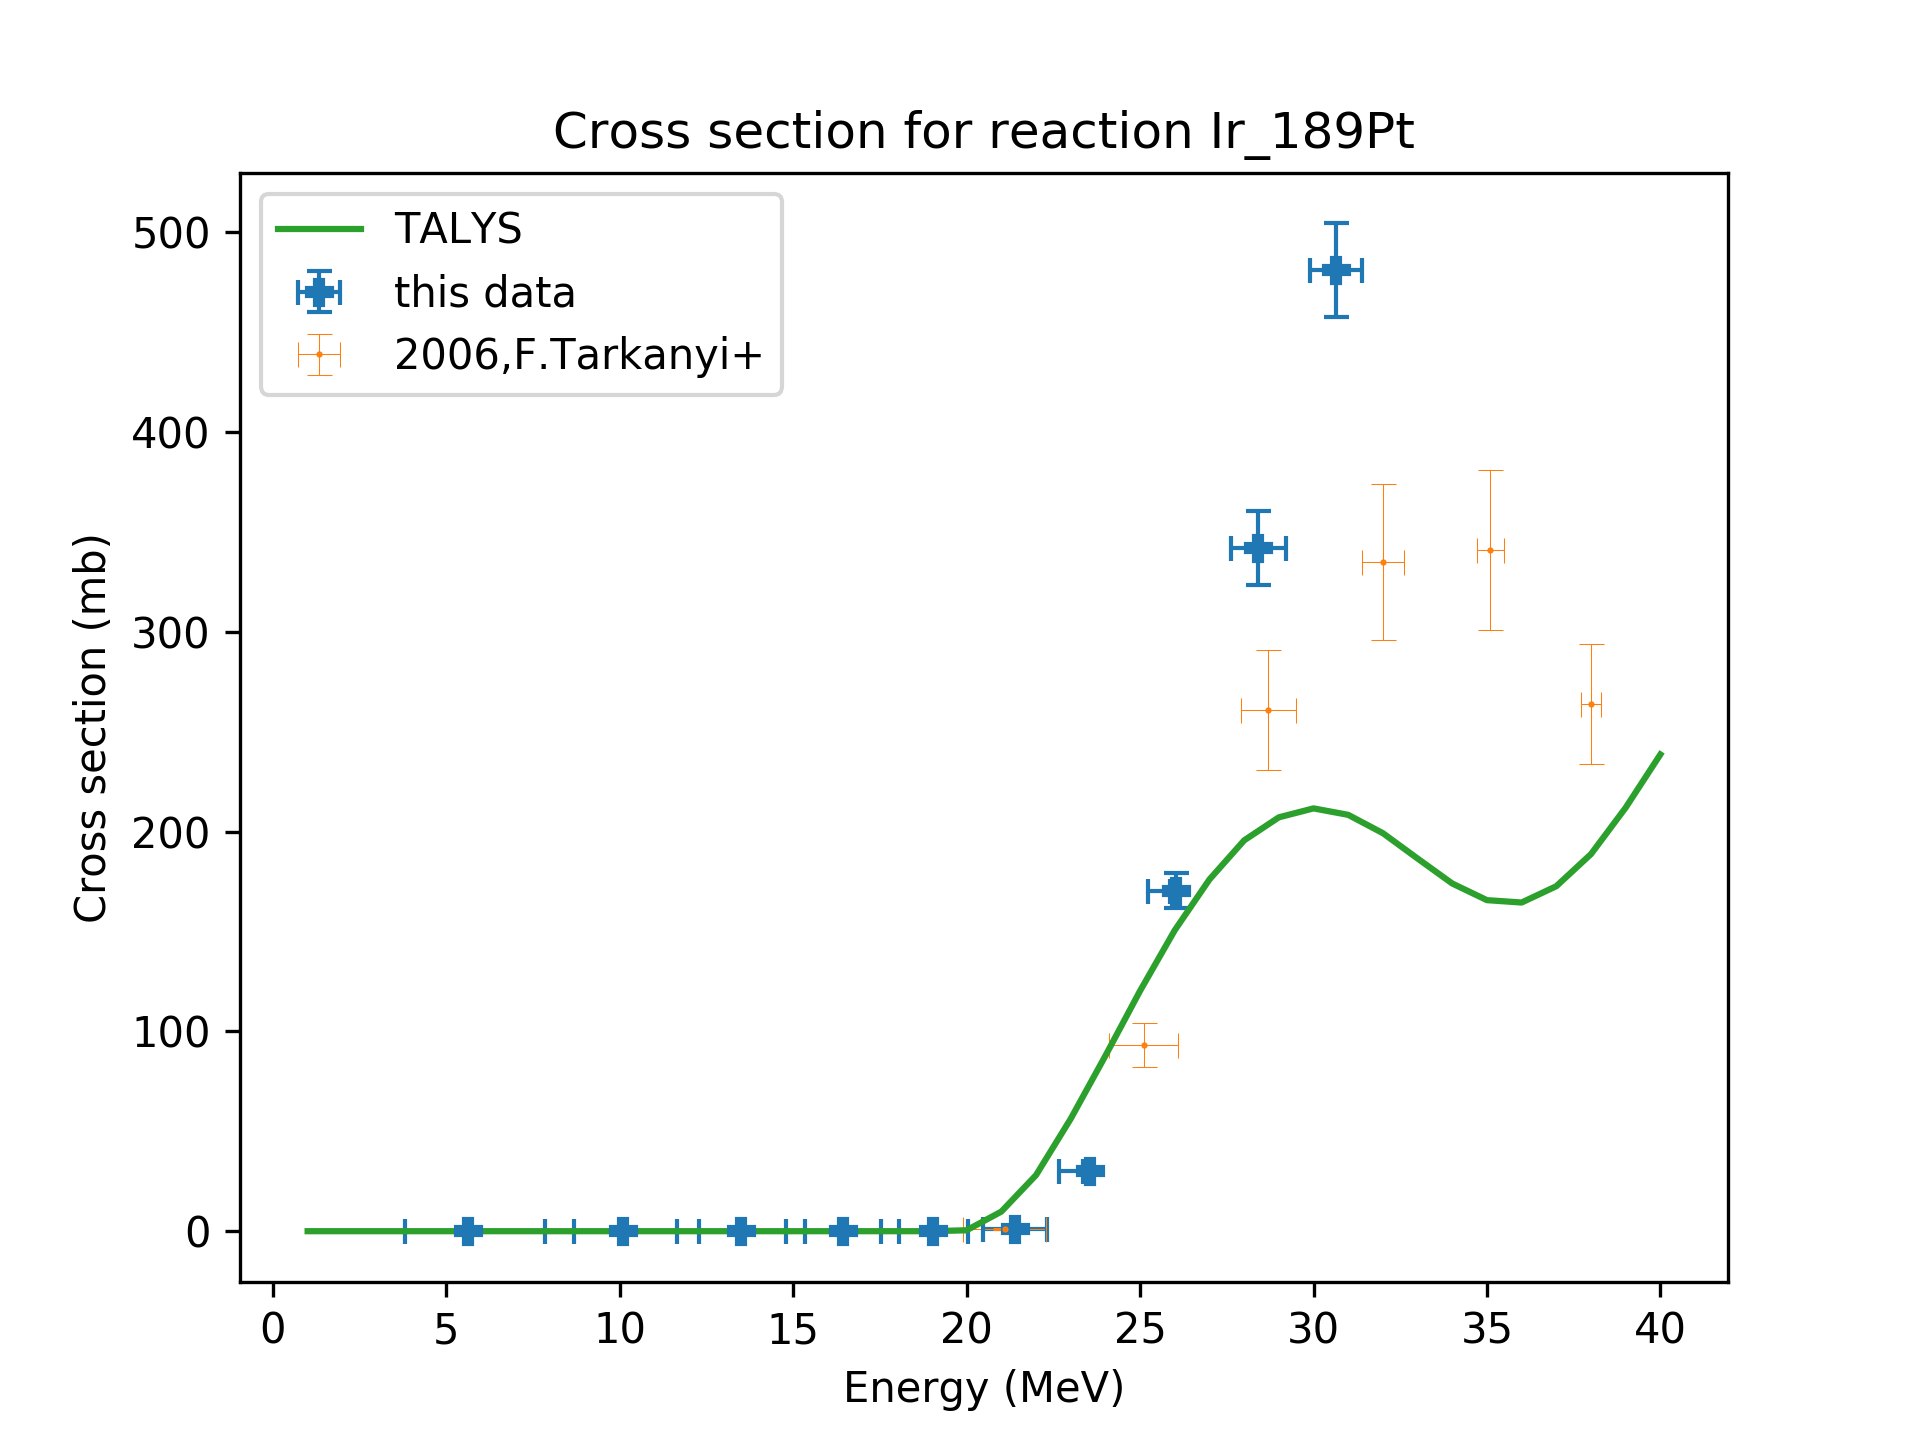
\includegraphics[width=5cm]{Results/Ir_189Pt.png} }}%
    \quad
    \subfloat[]{{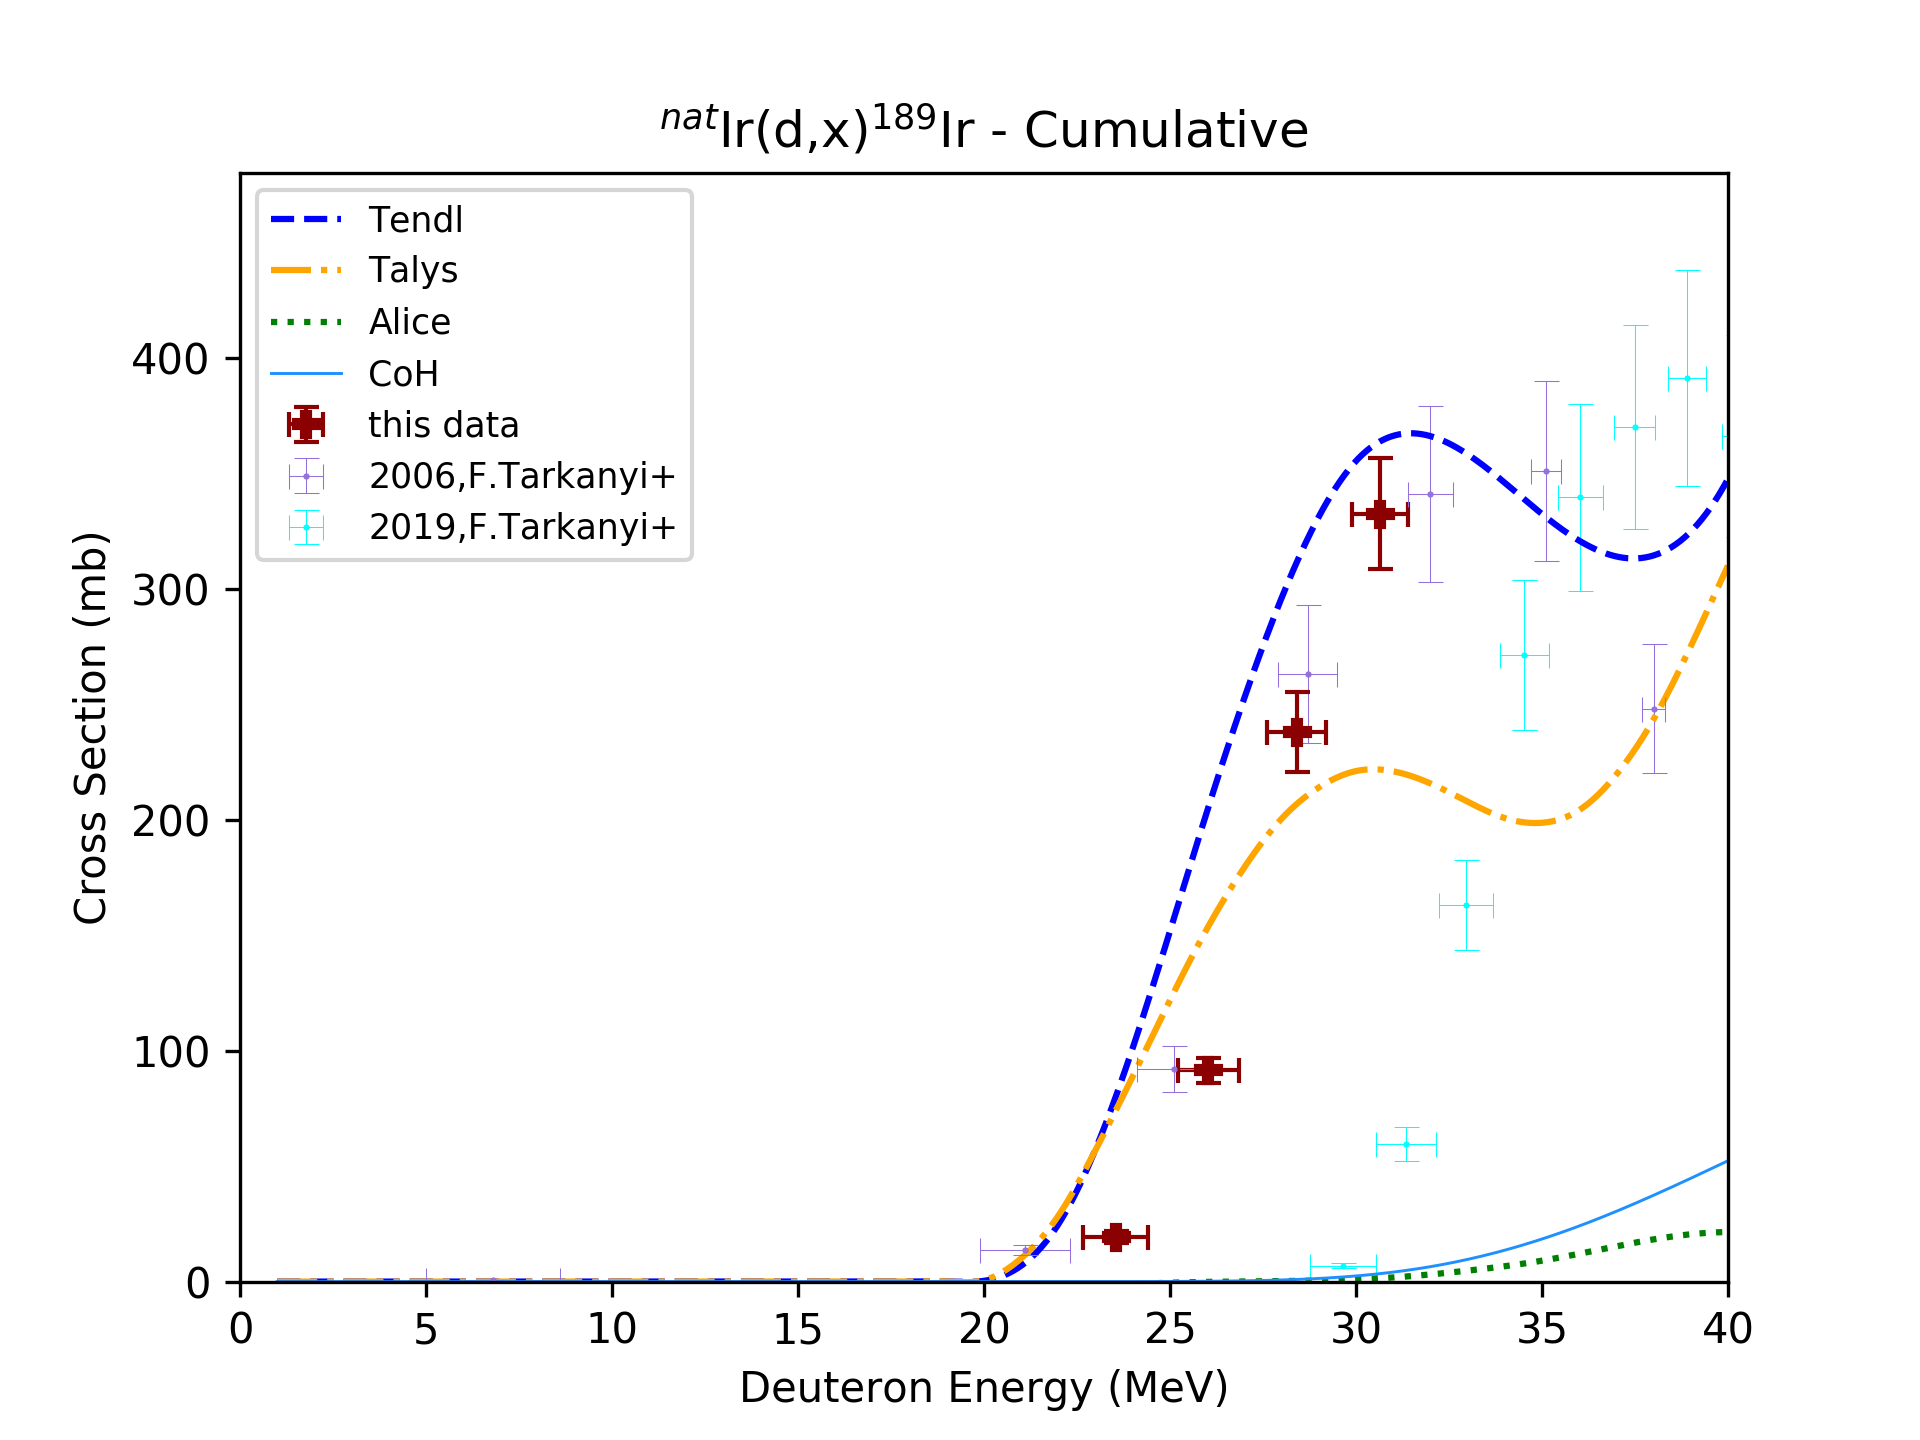
\includegraphics[width=5cm]{Results/Ir_189Ir.png} }}%
    \quad
    \subfloat[]{{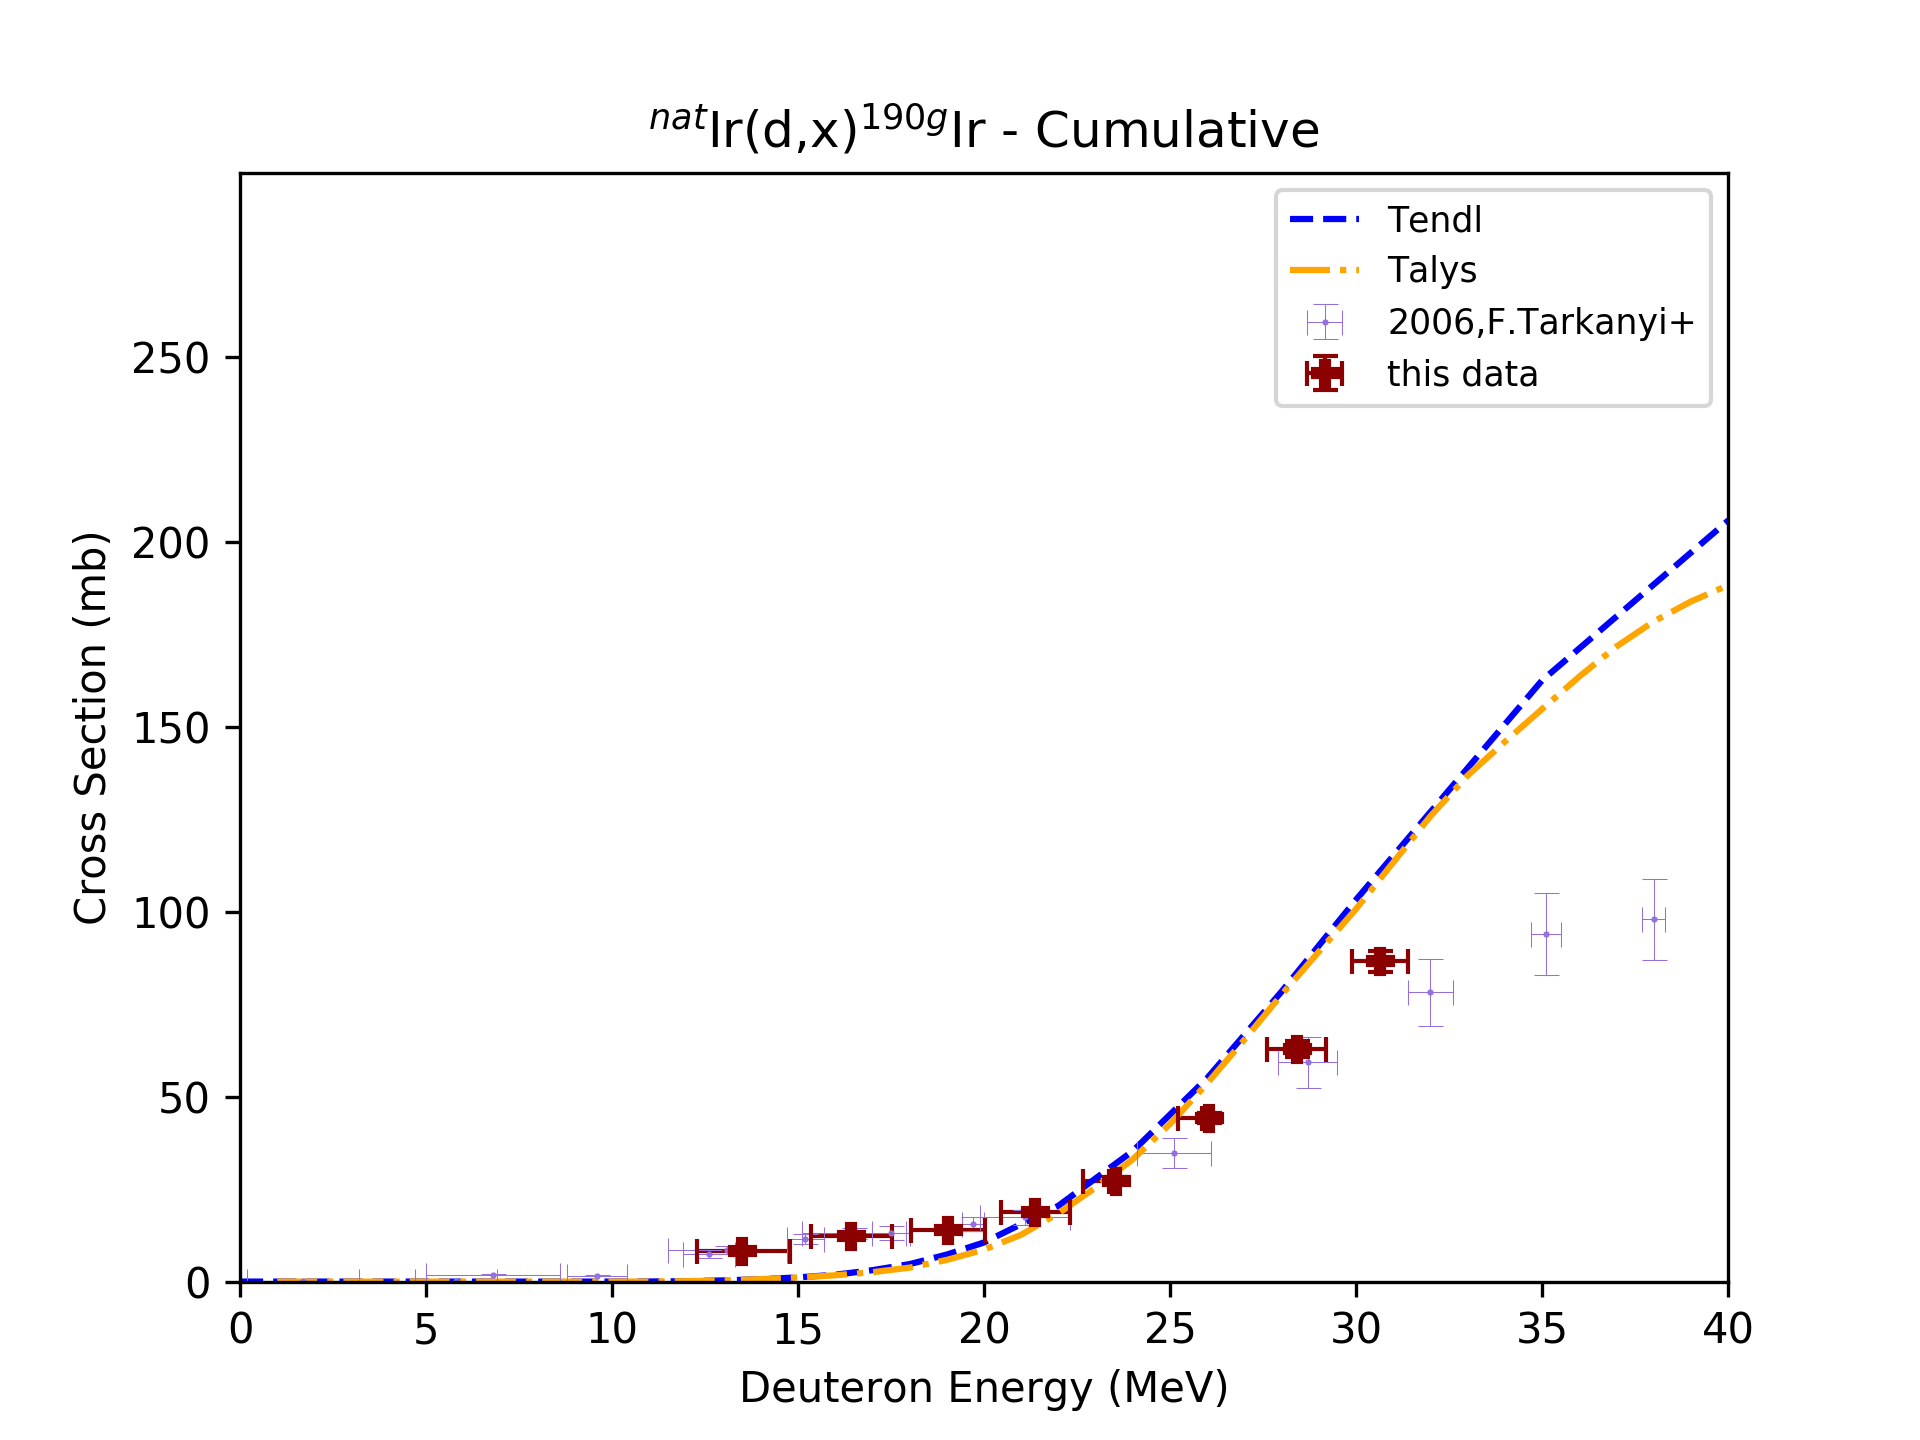
\includegraphics[width=5cm]{Results/Ir_190Ir.png} }}%
    \quad
    \subfloat[caption]{{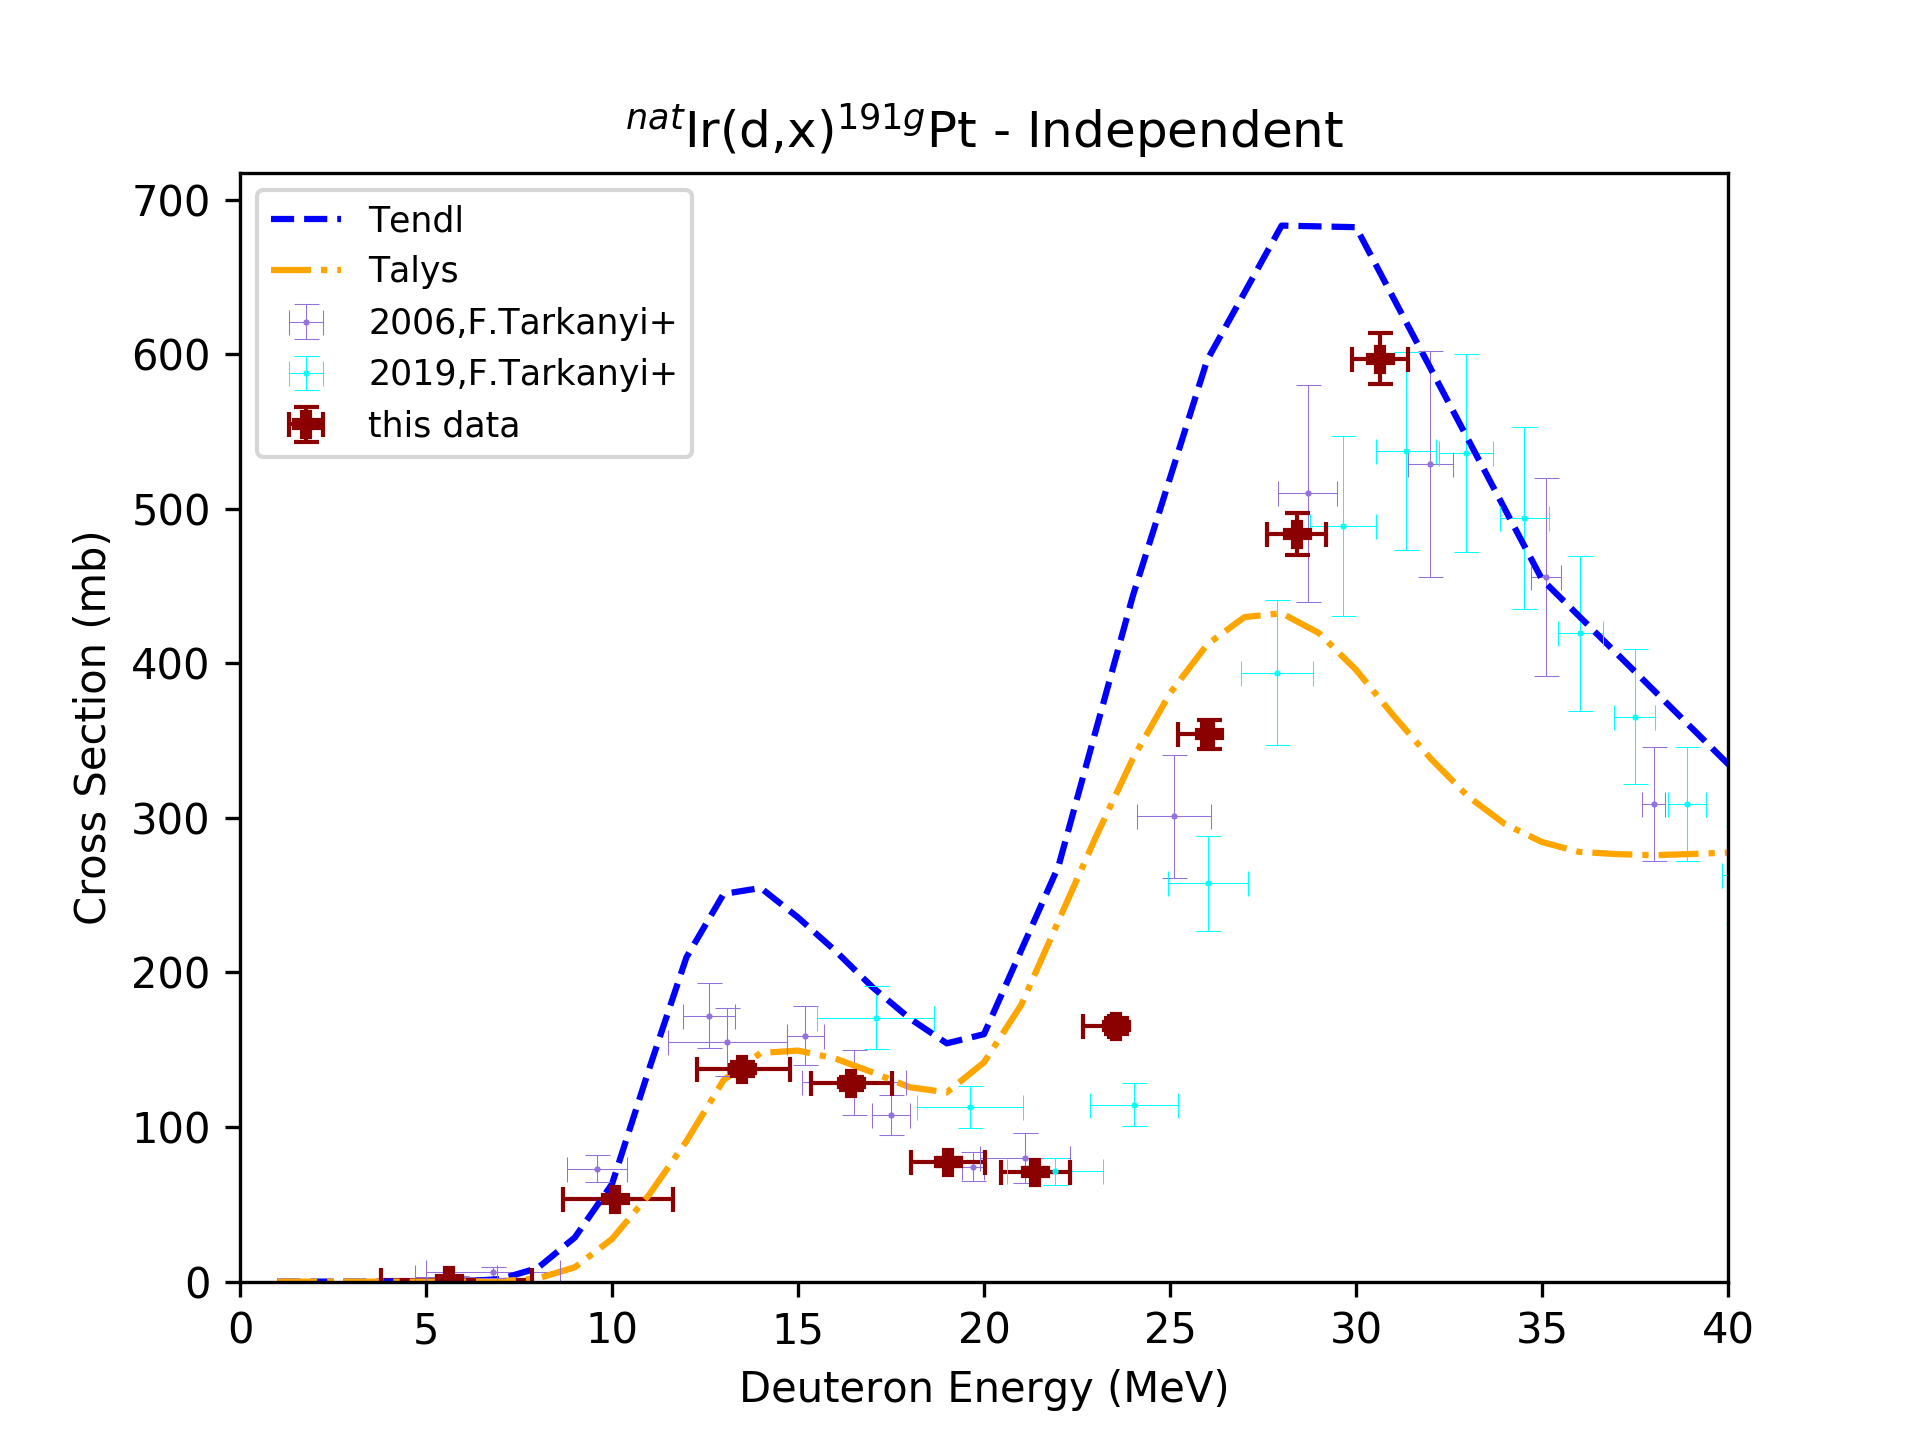
\includegraphics[width=5cm]{Results/Ir_191Pt.png} }}%
    \quad
    \subfloat[]{{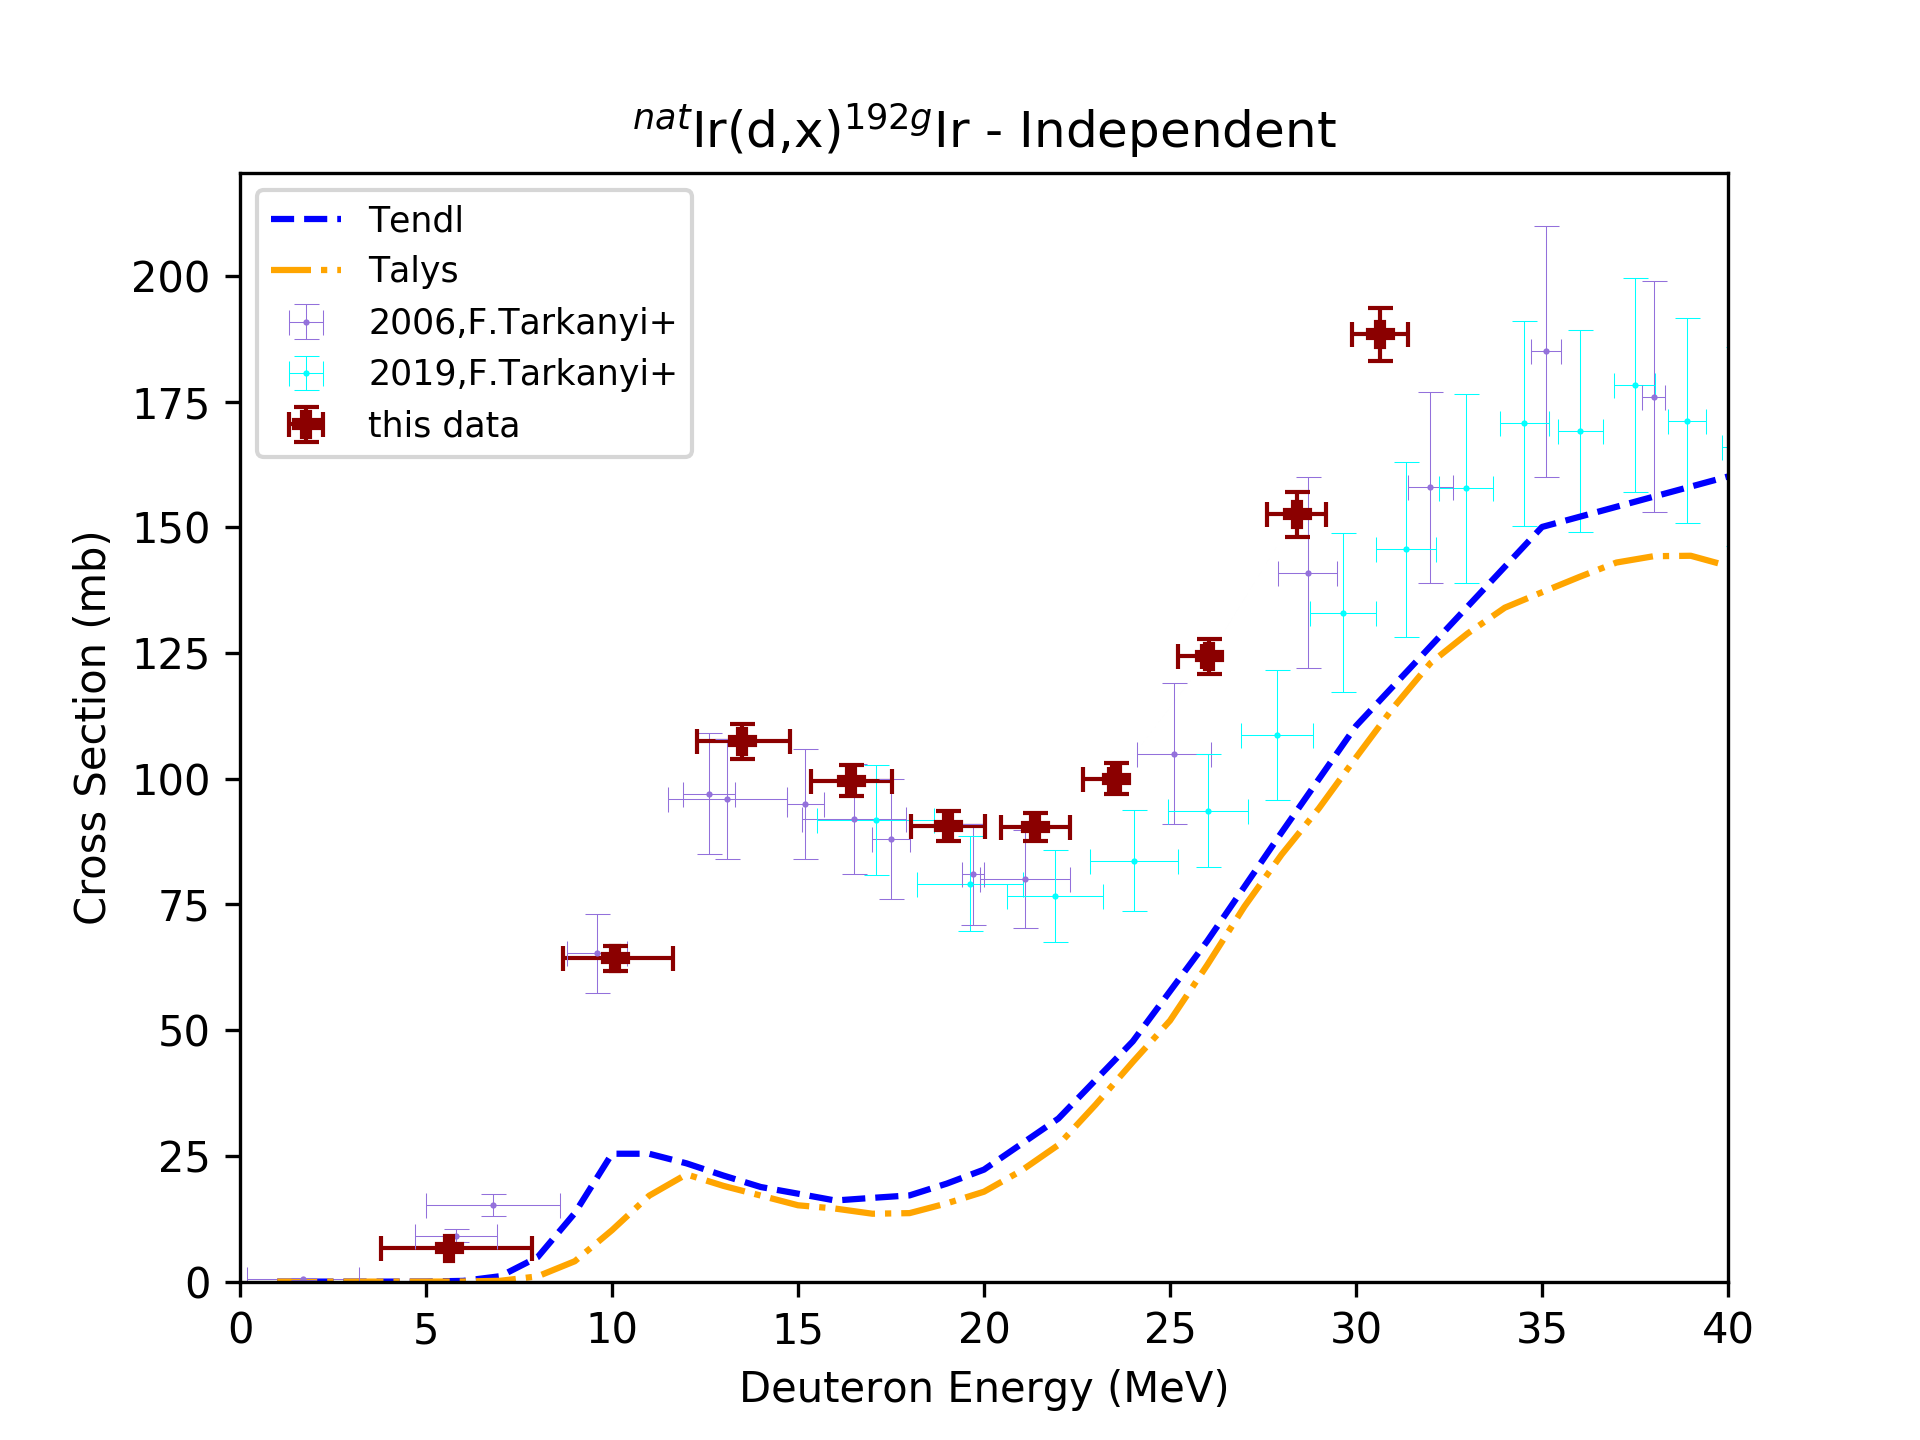
\includegraphics[width=5cm]{Results/Ir_192Ir.png} }}%
    \quad
    \subfloat[]{{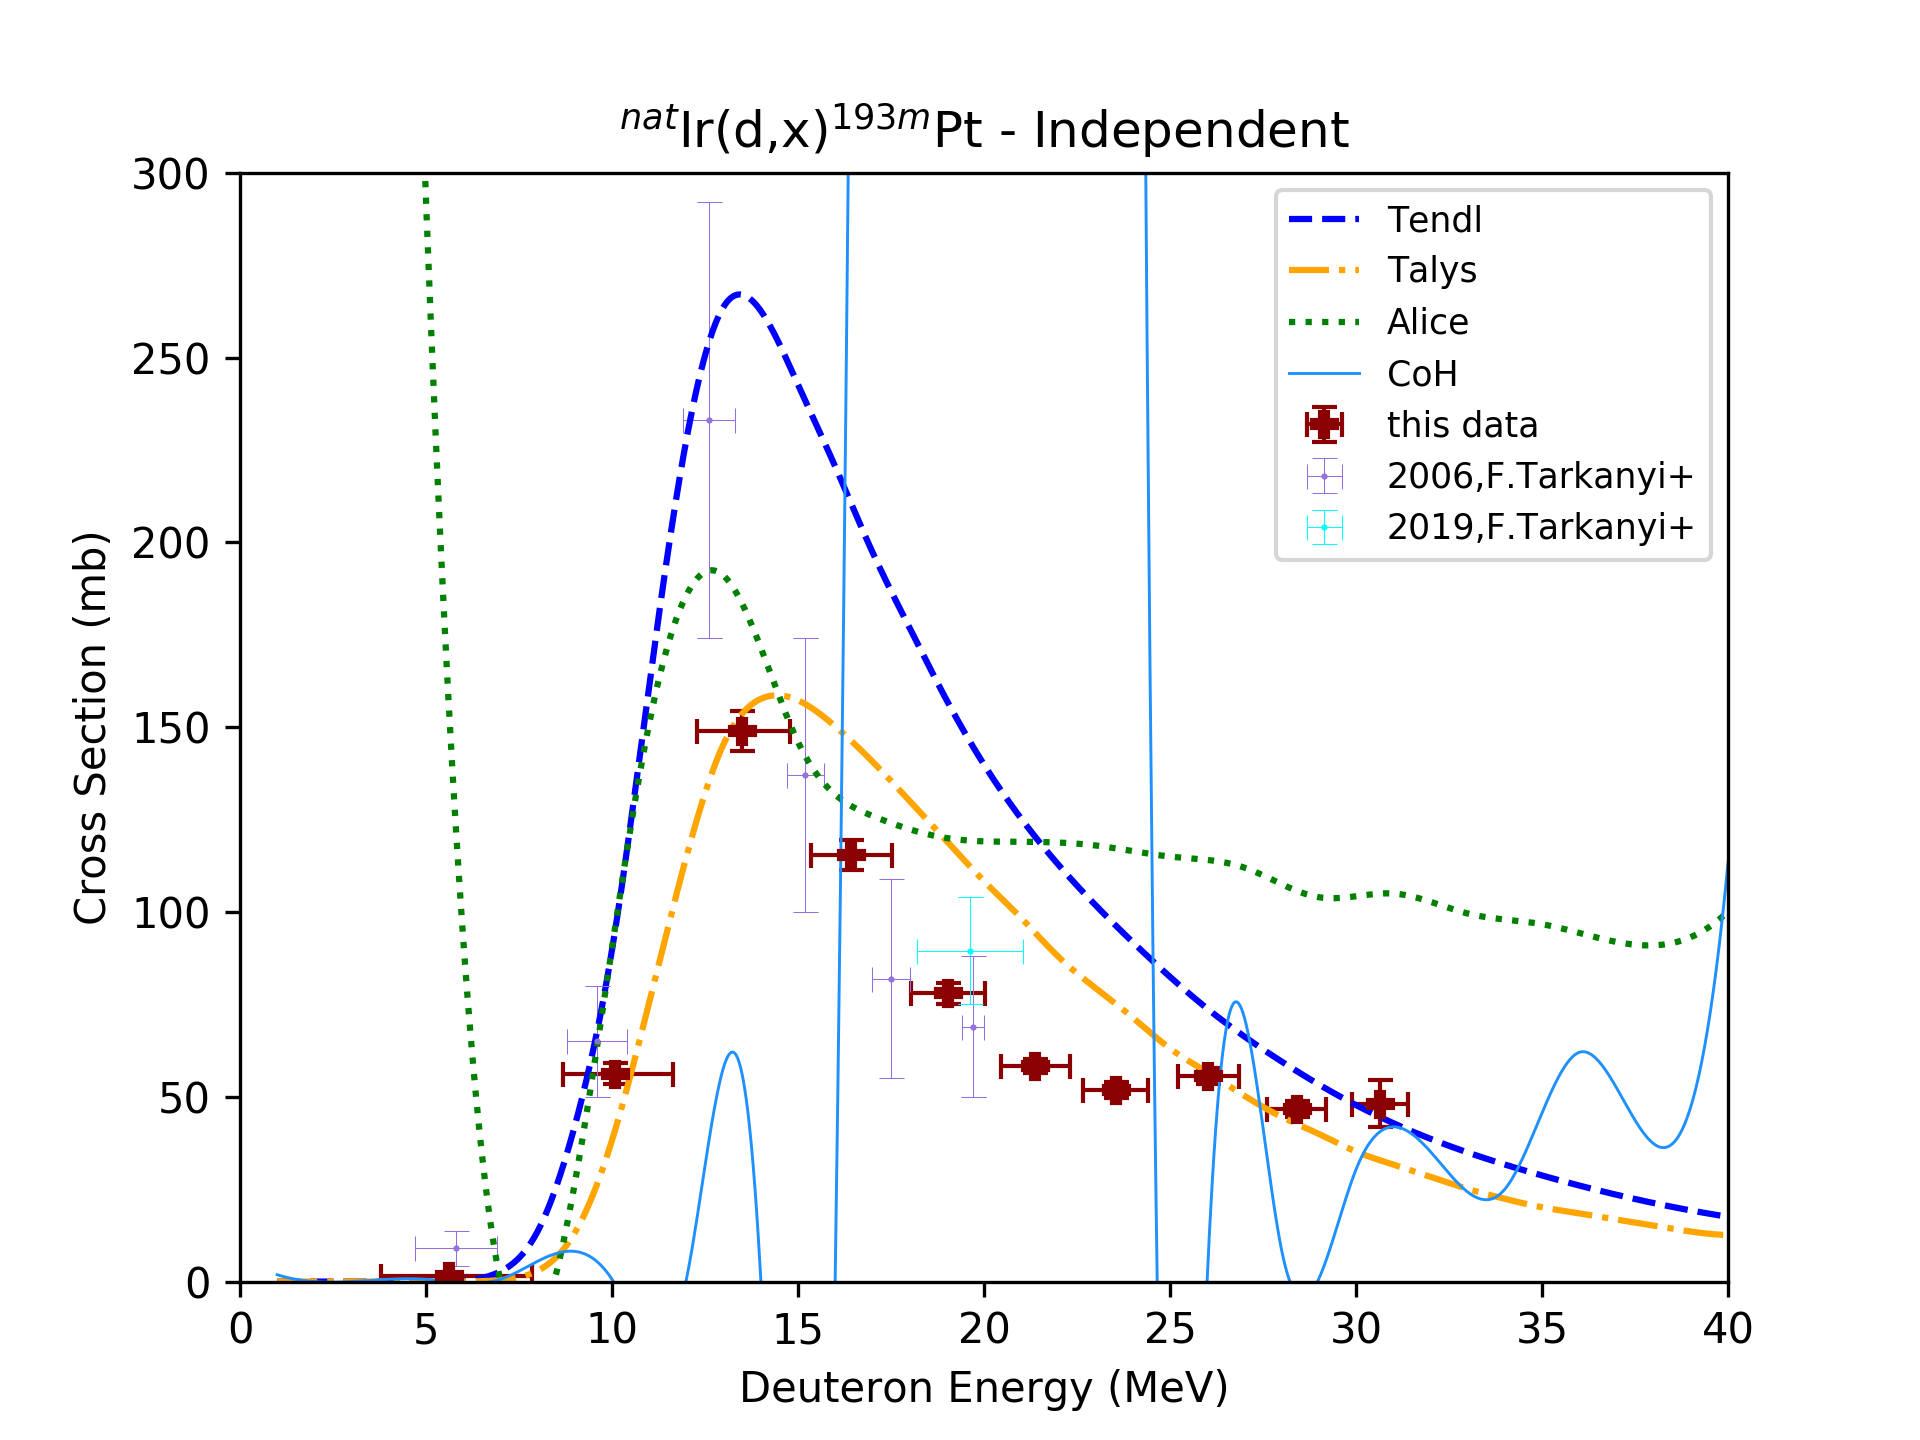
\includegraphics[width=5cm]{Results/Ir_193mPt.png} }}%
    \quad
    \subfloat[]{{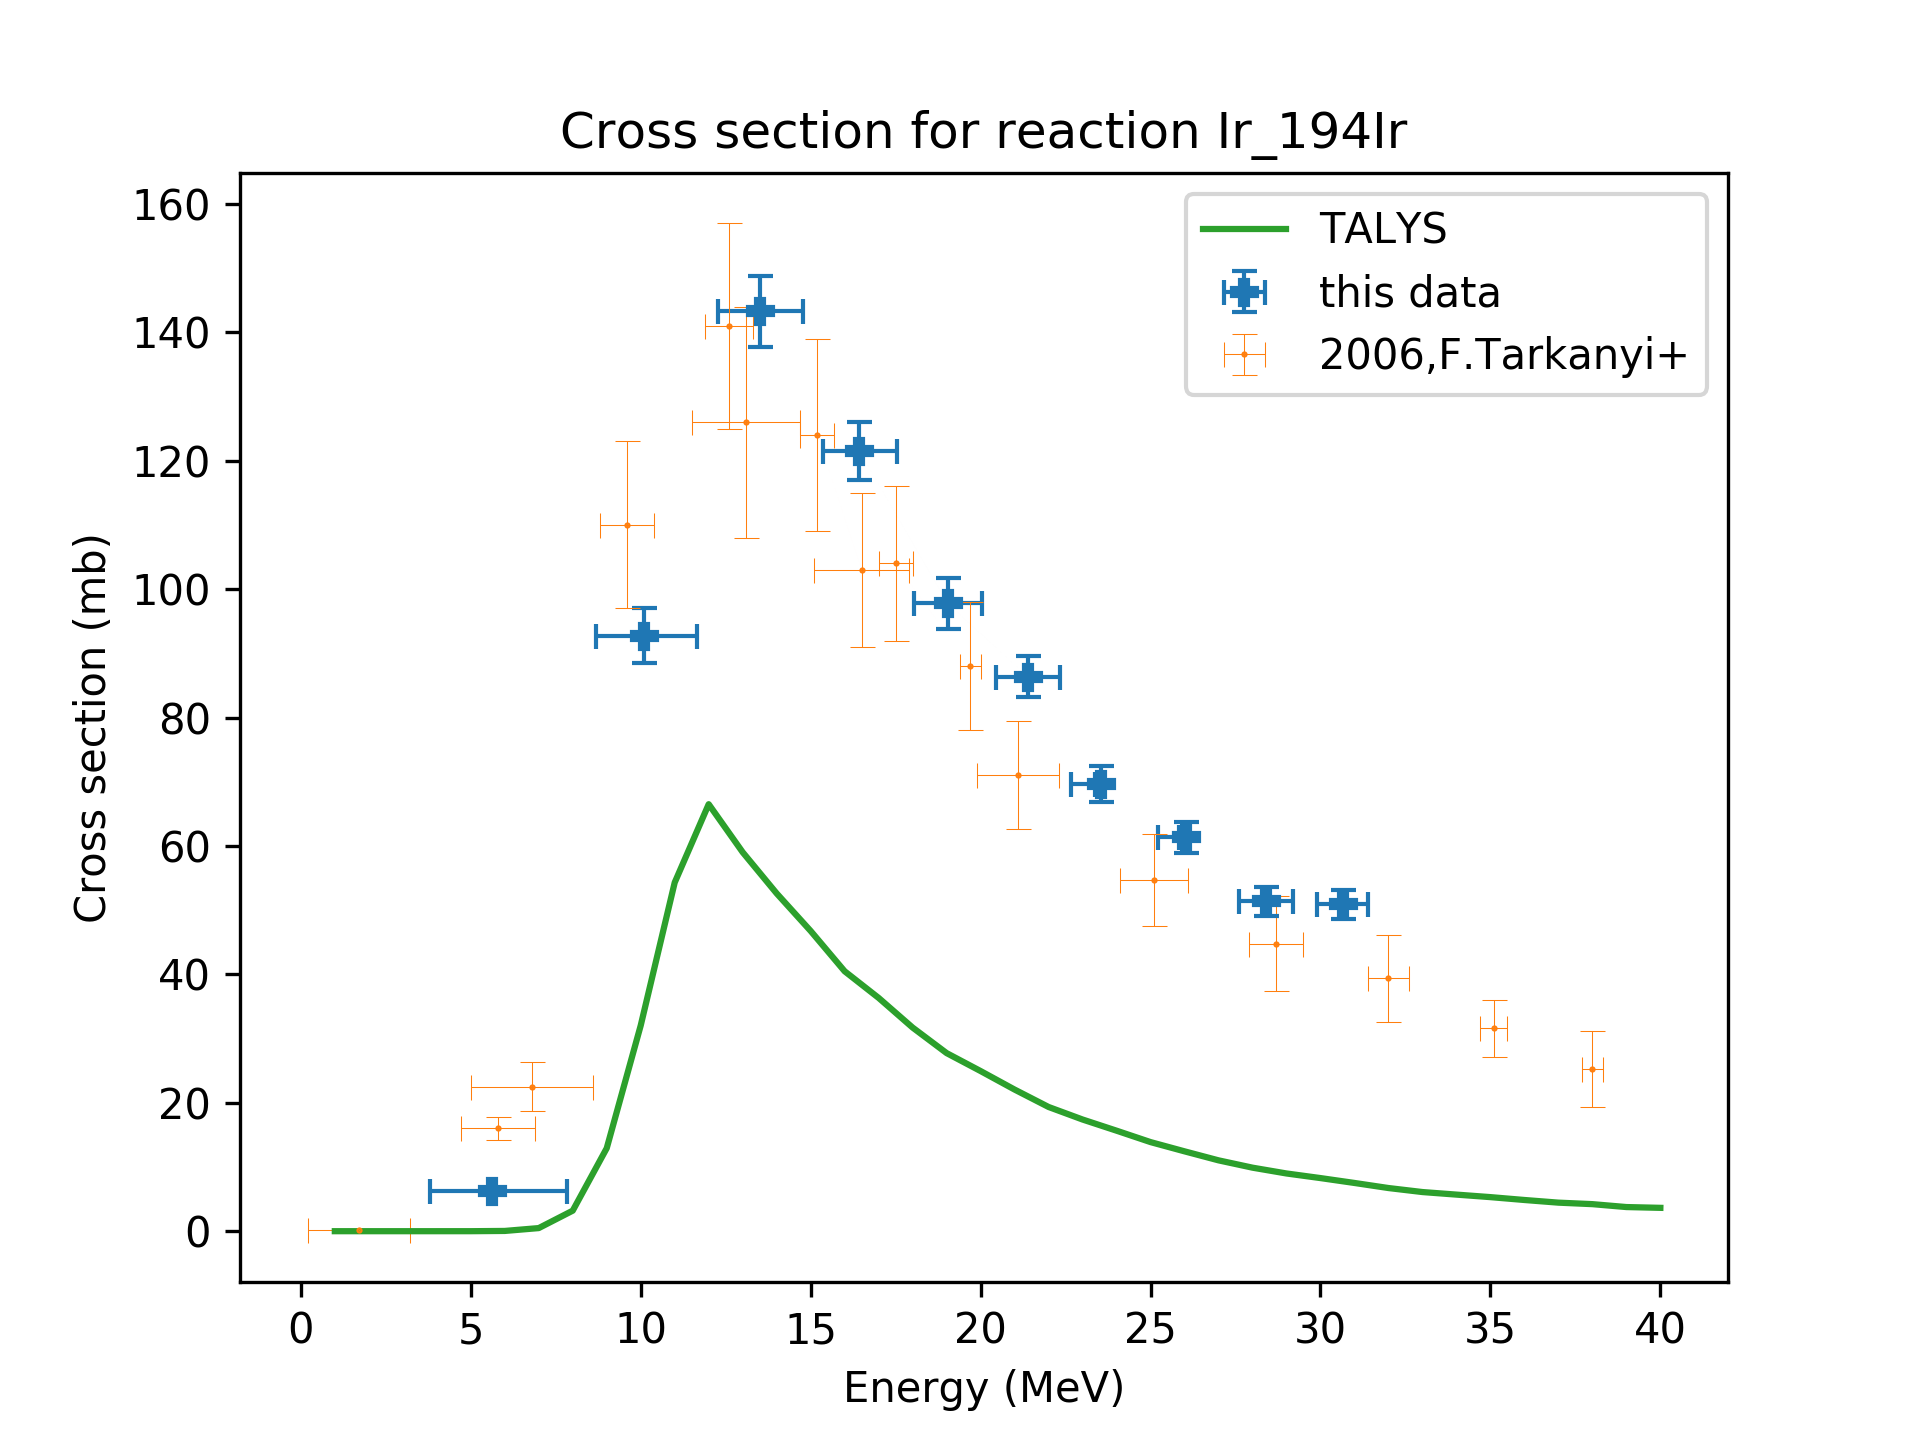
\includegraphics[width=5cm]{Results/Ir_194Ir.png} }}%
    \quad
    \subfloat[]{{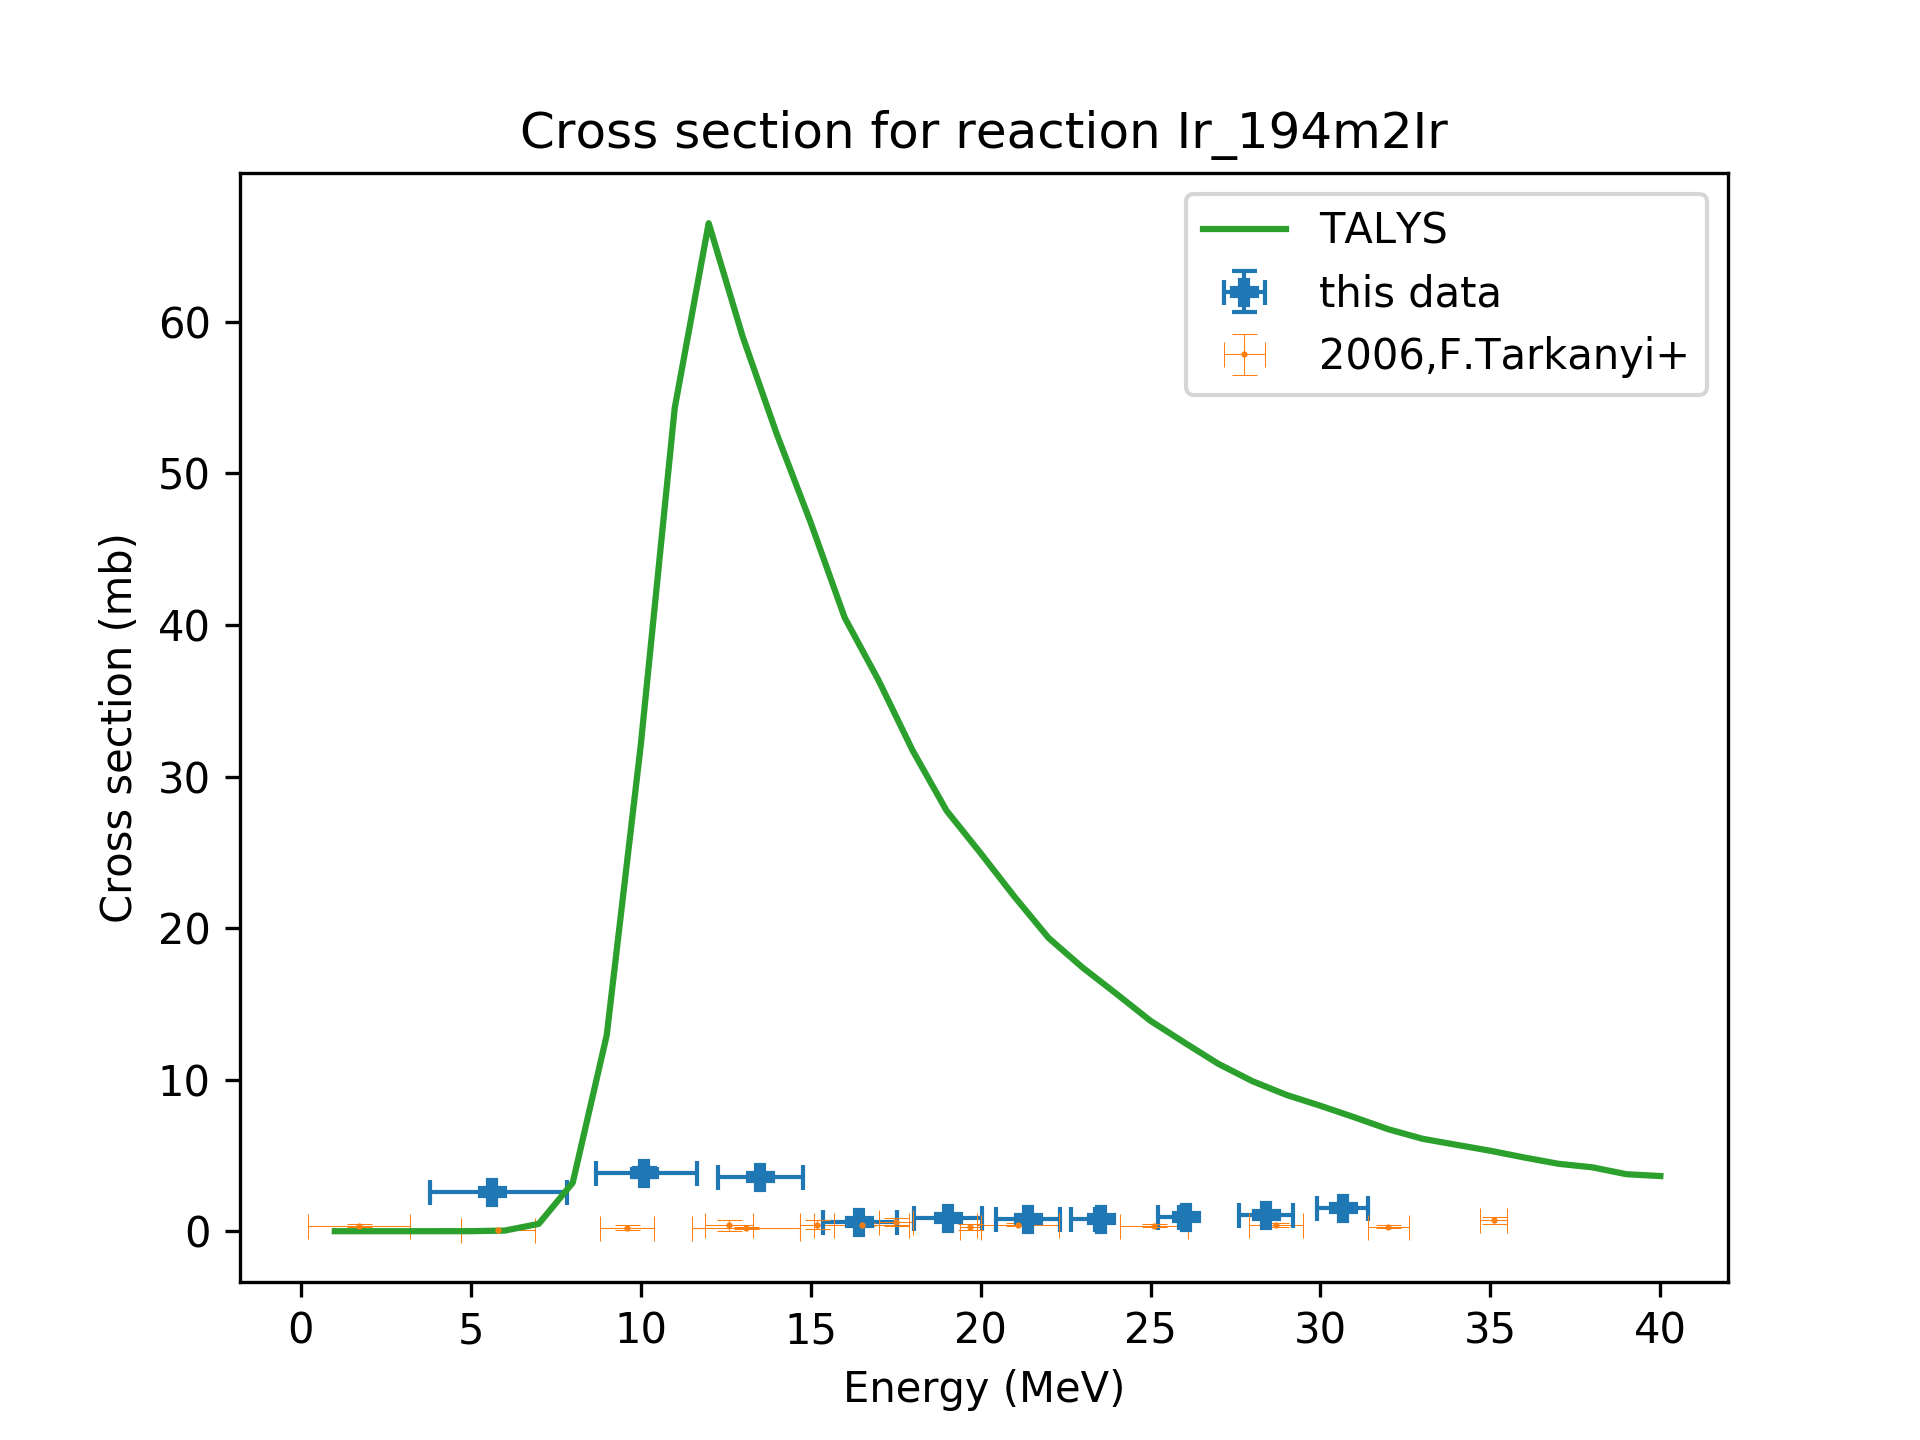
\includegraphics[width=5cm]{Results/Ir_194m2Ir.png} }}%
    \quad
    \caption{Iridium cross sections }%
    \label{fig:Ir_crosssections}%
\end{figure}

\section{Nickel cross sections}

\begin{figure}%
    \centering
    \subfloat[]{{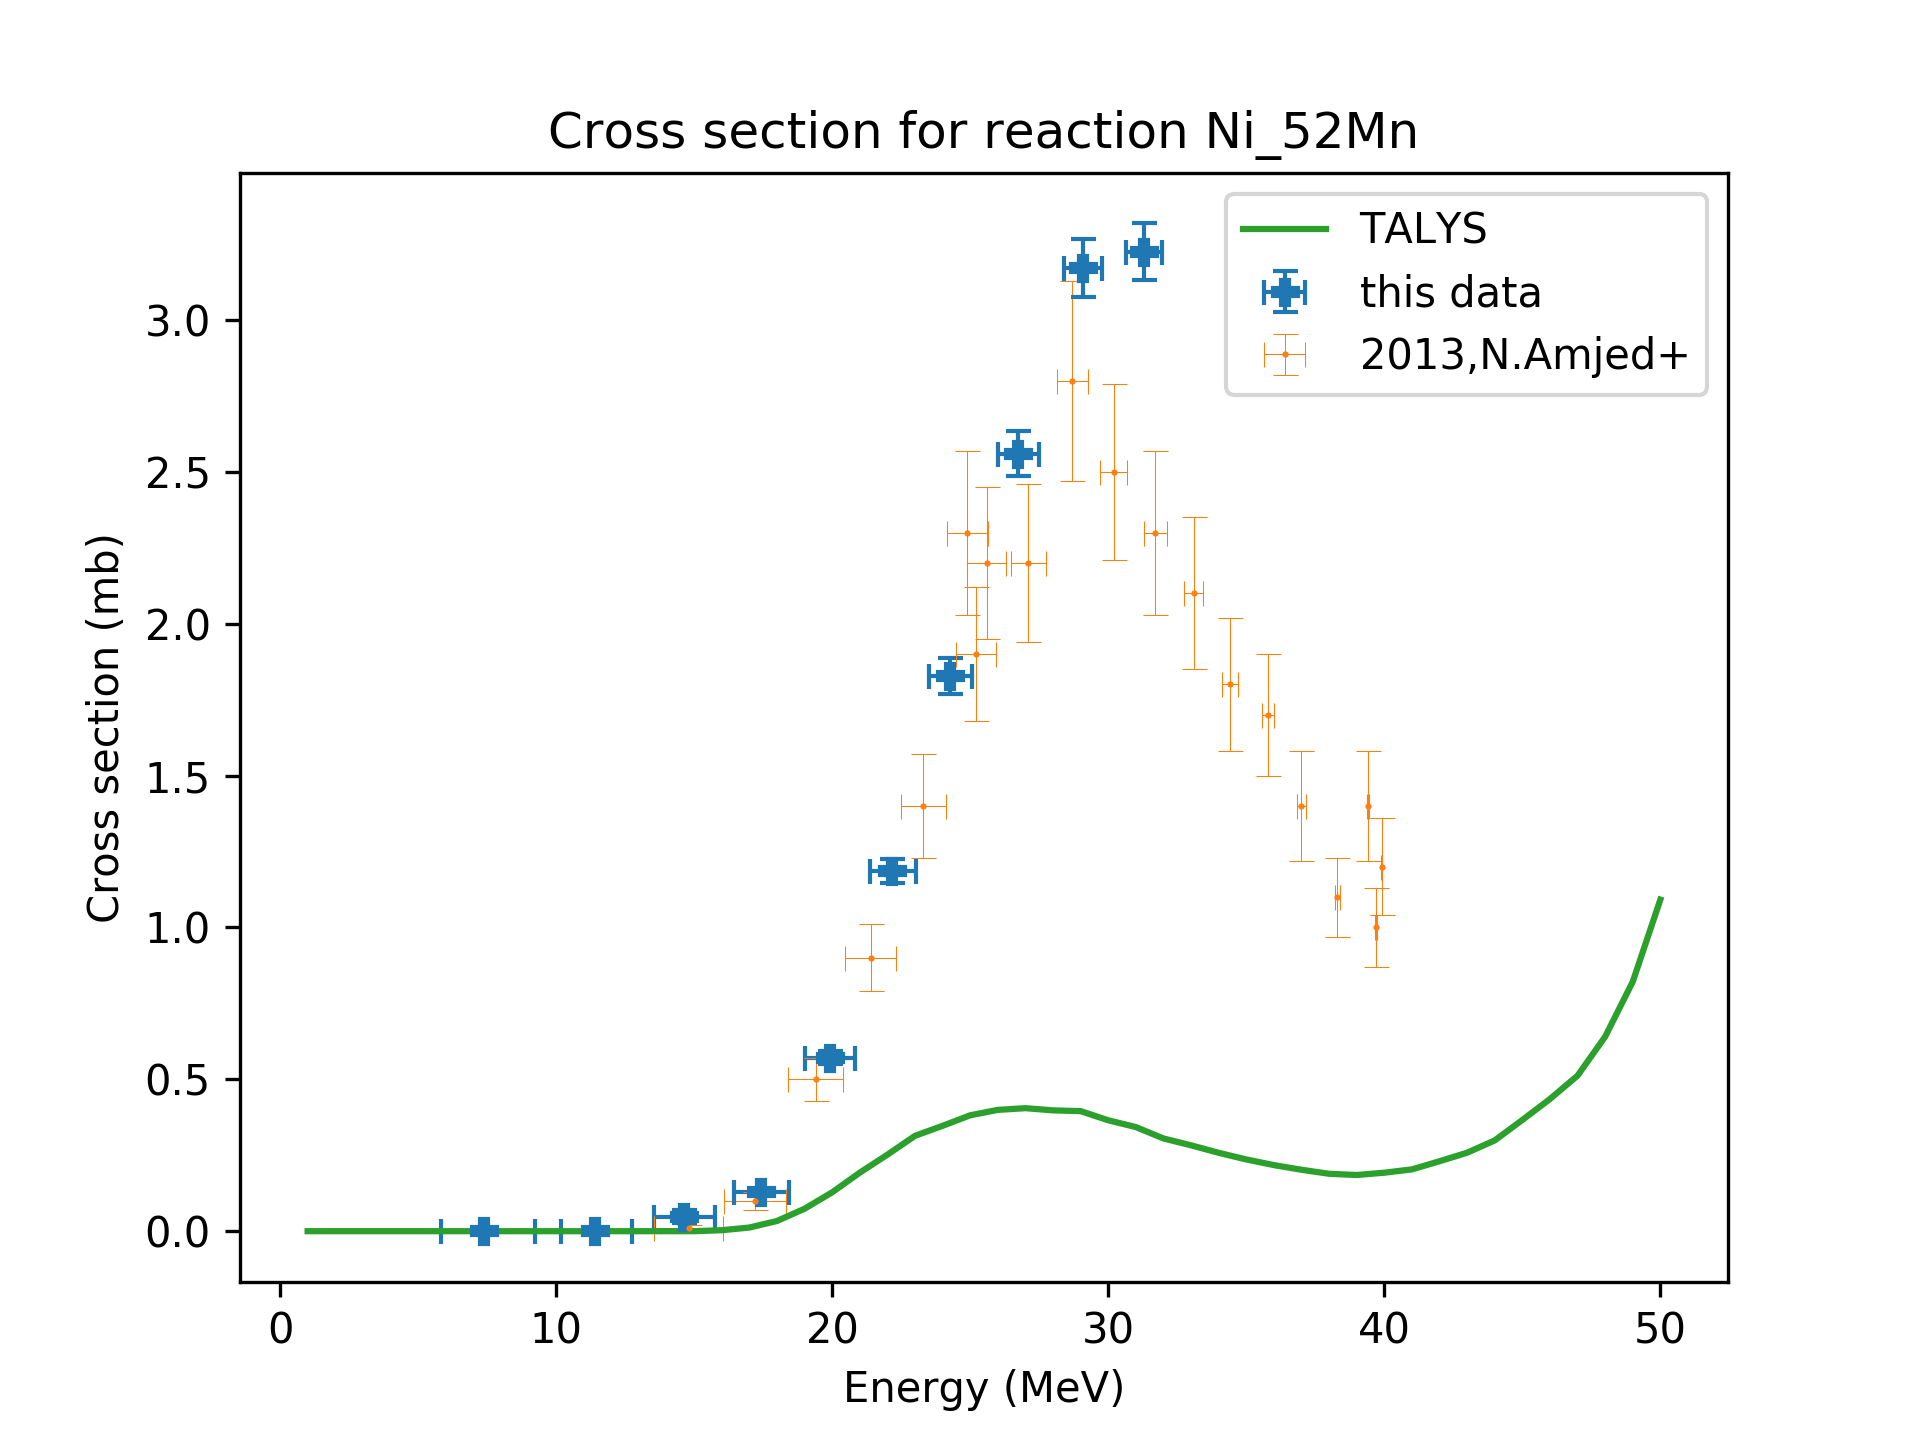
\includegraphics[width=5cm]{Results/Ni_52Mn.png}}%
    \quad
    \subfloat[]{{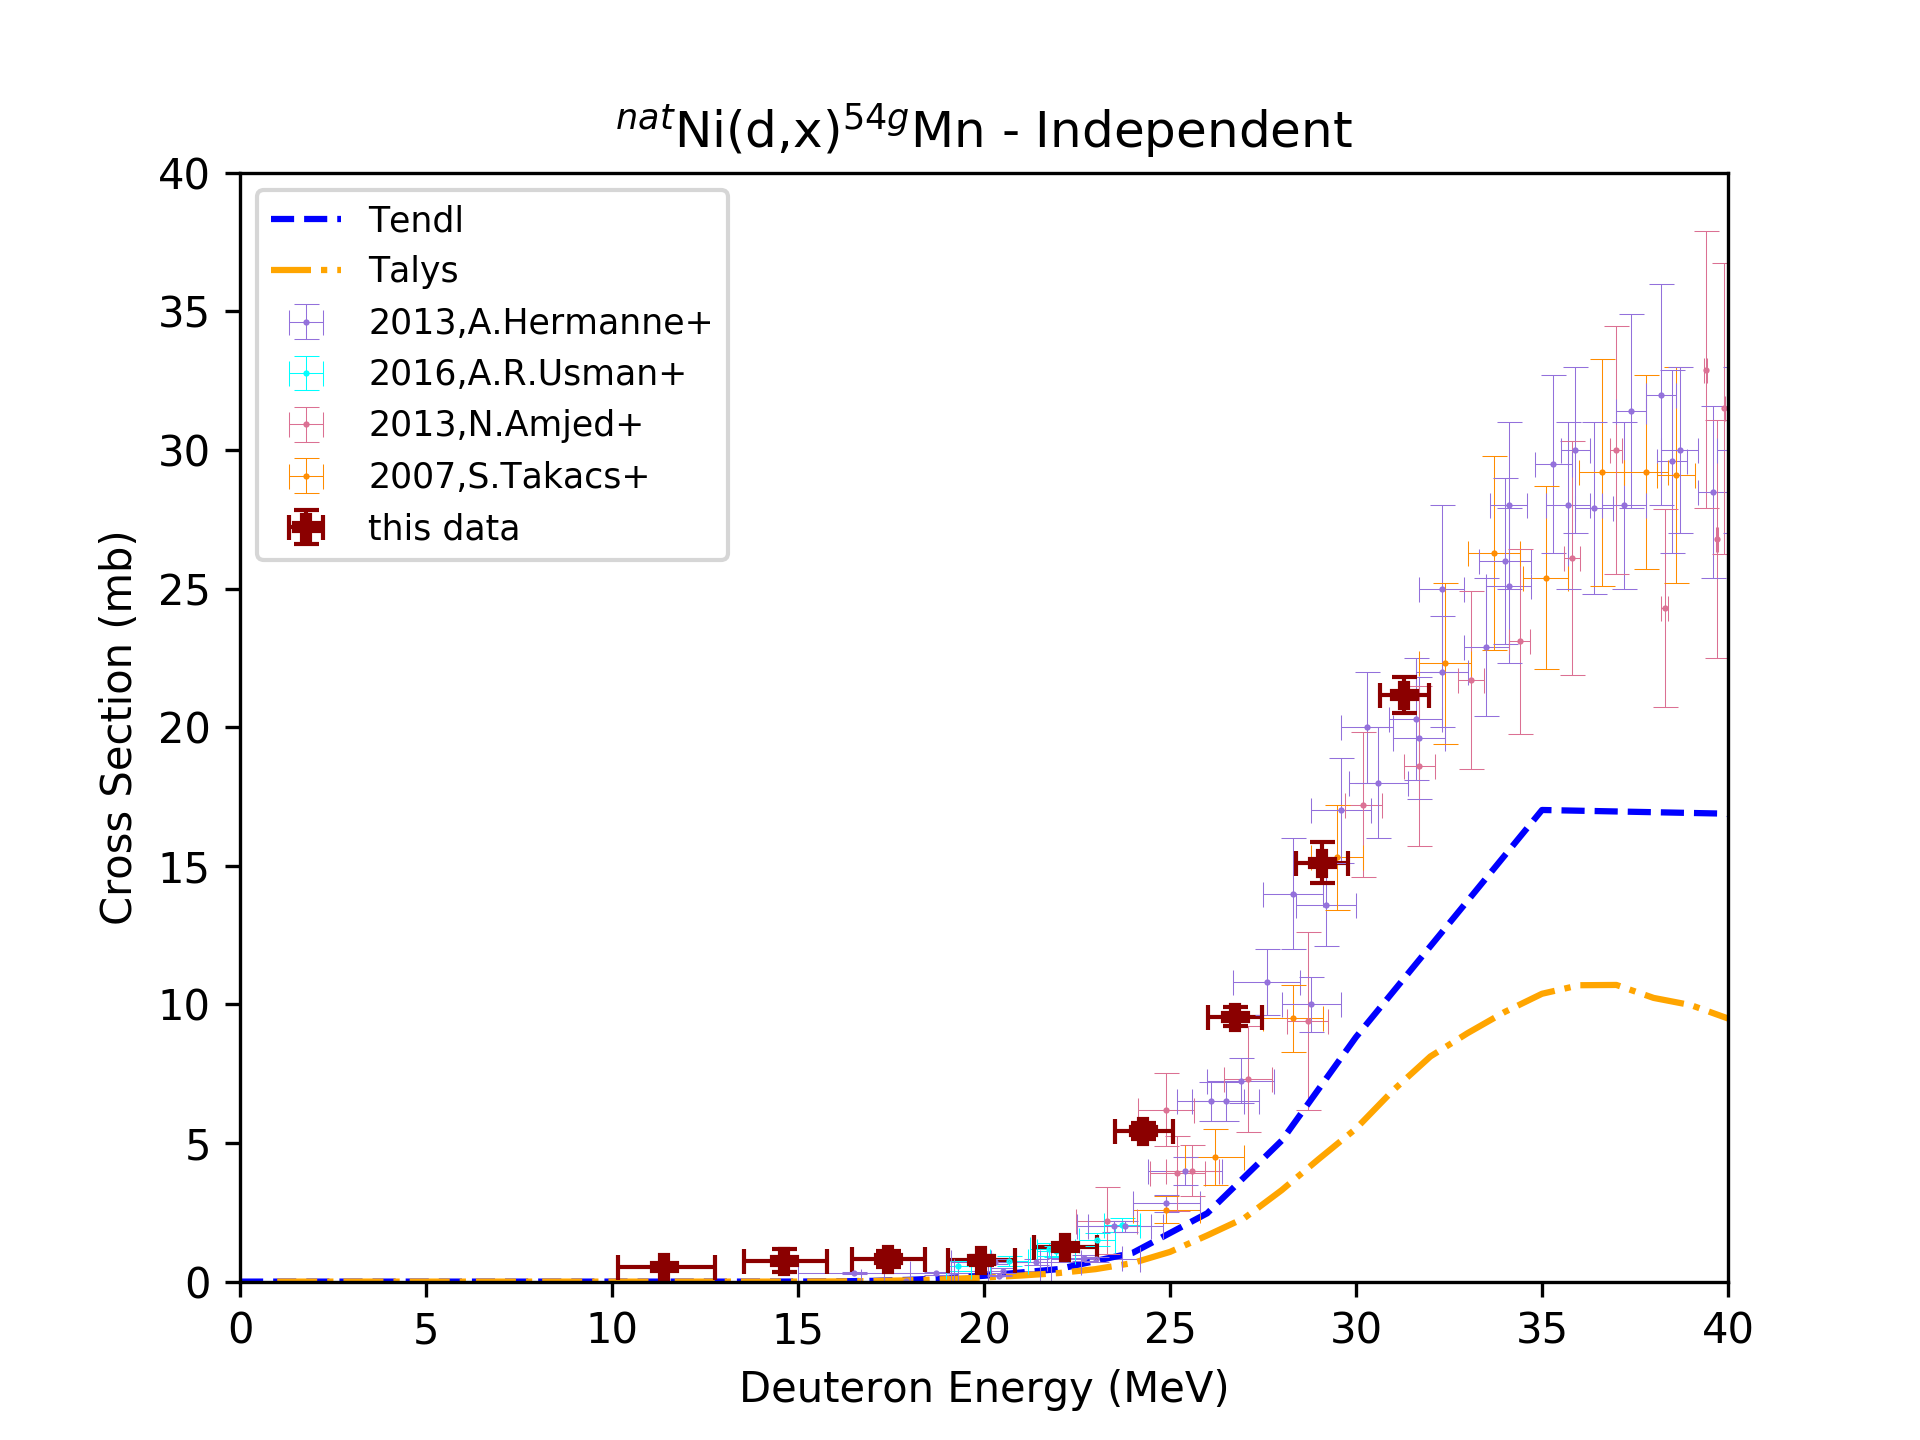
\includegraphics[width=5cm]{Results/Ni_54Mn.png} }}%
    \subfloat[]{{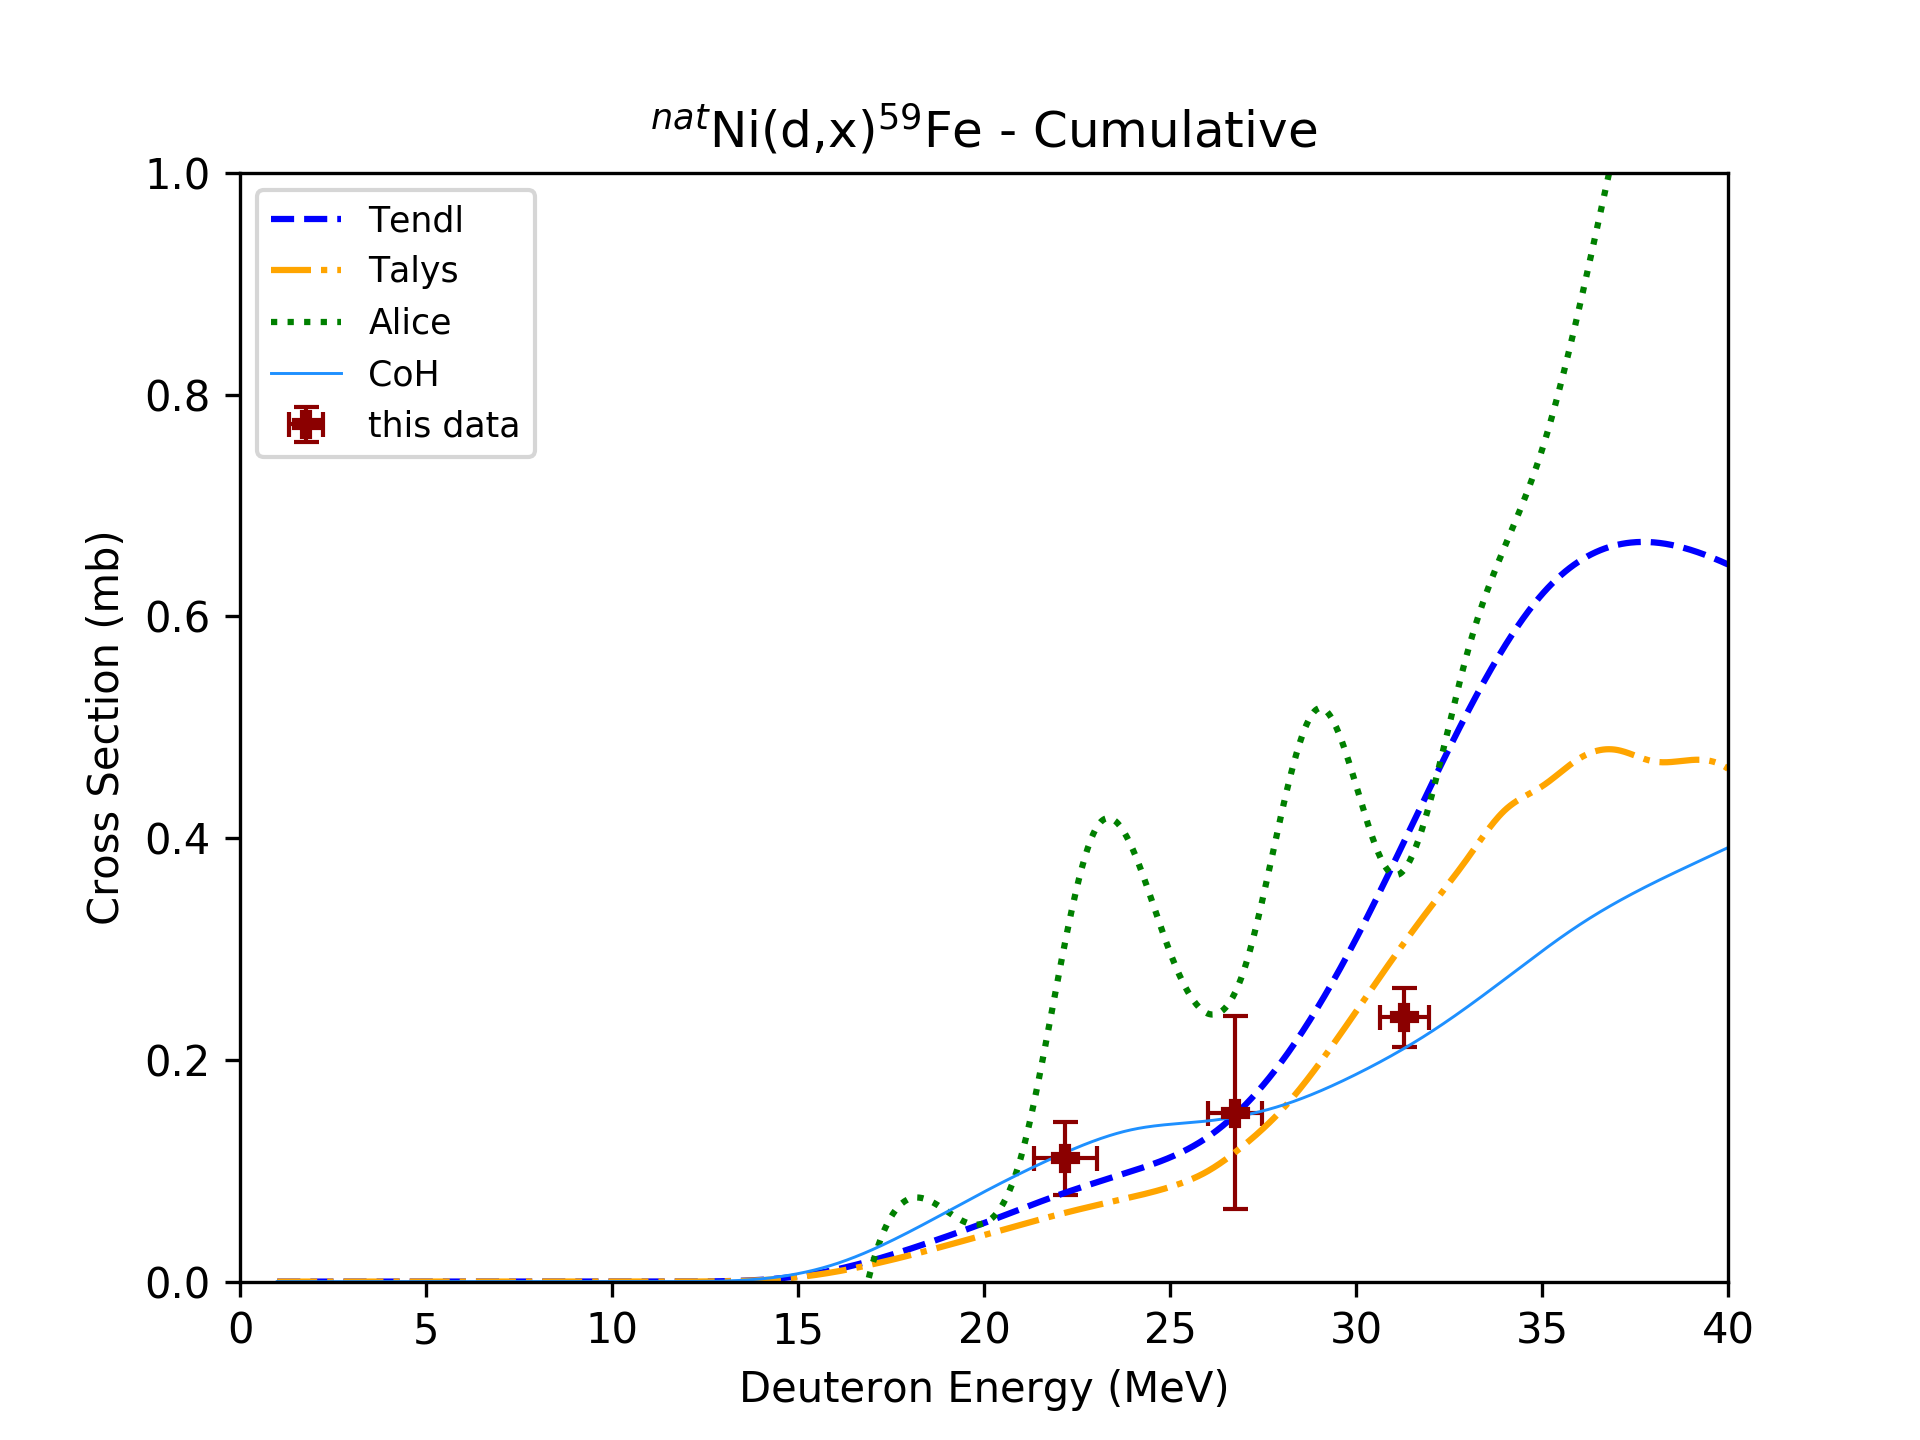
\includegraphics[width=5cm]{Results/Ni_59Fe.png} }}%
    \quad
    \subfloat[]{{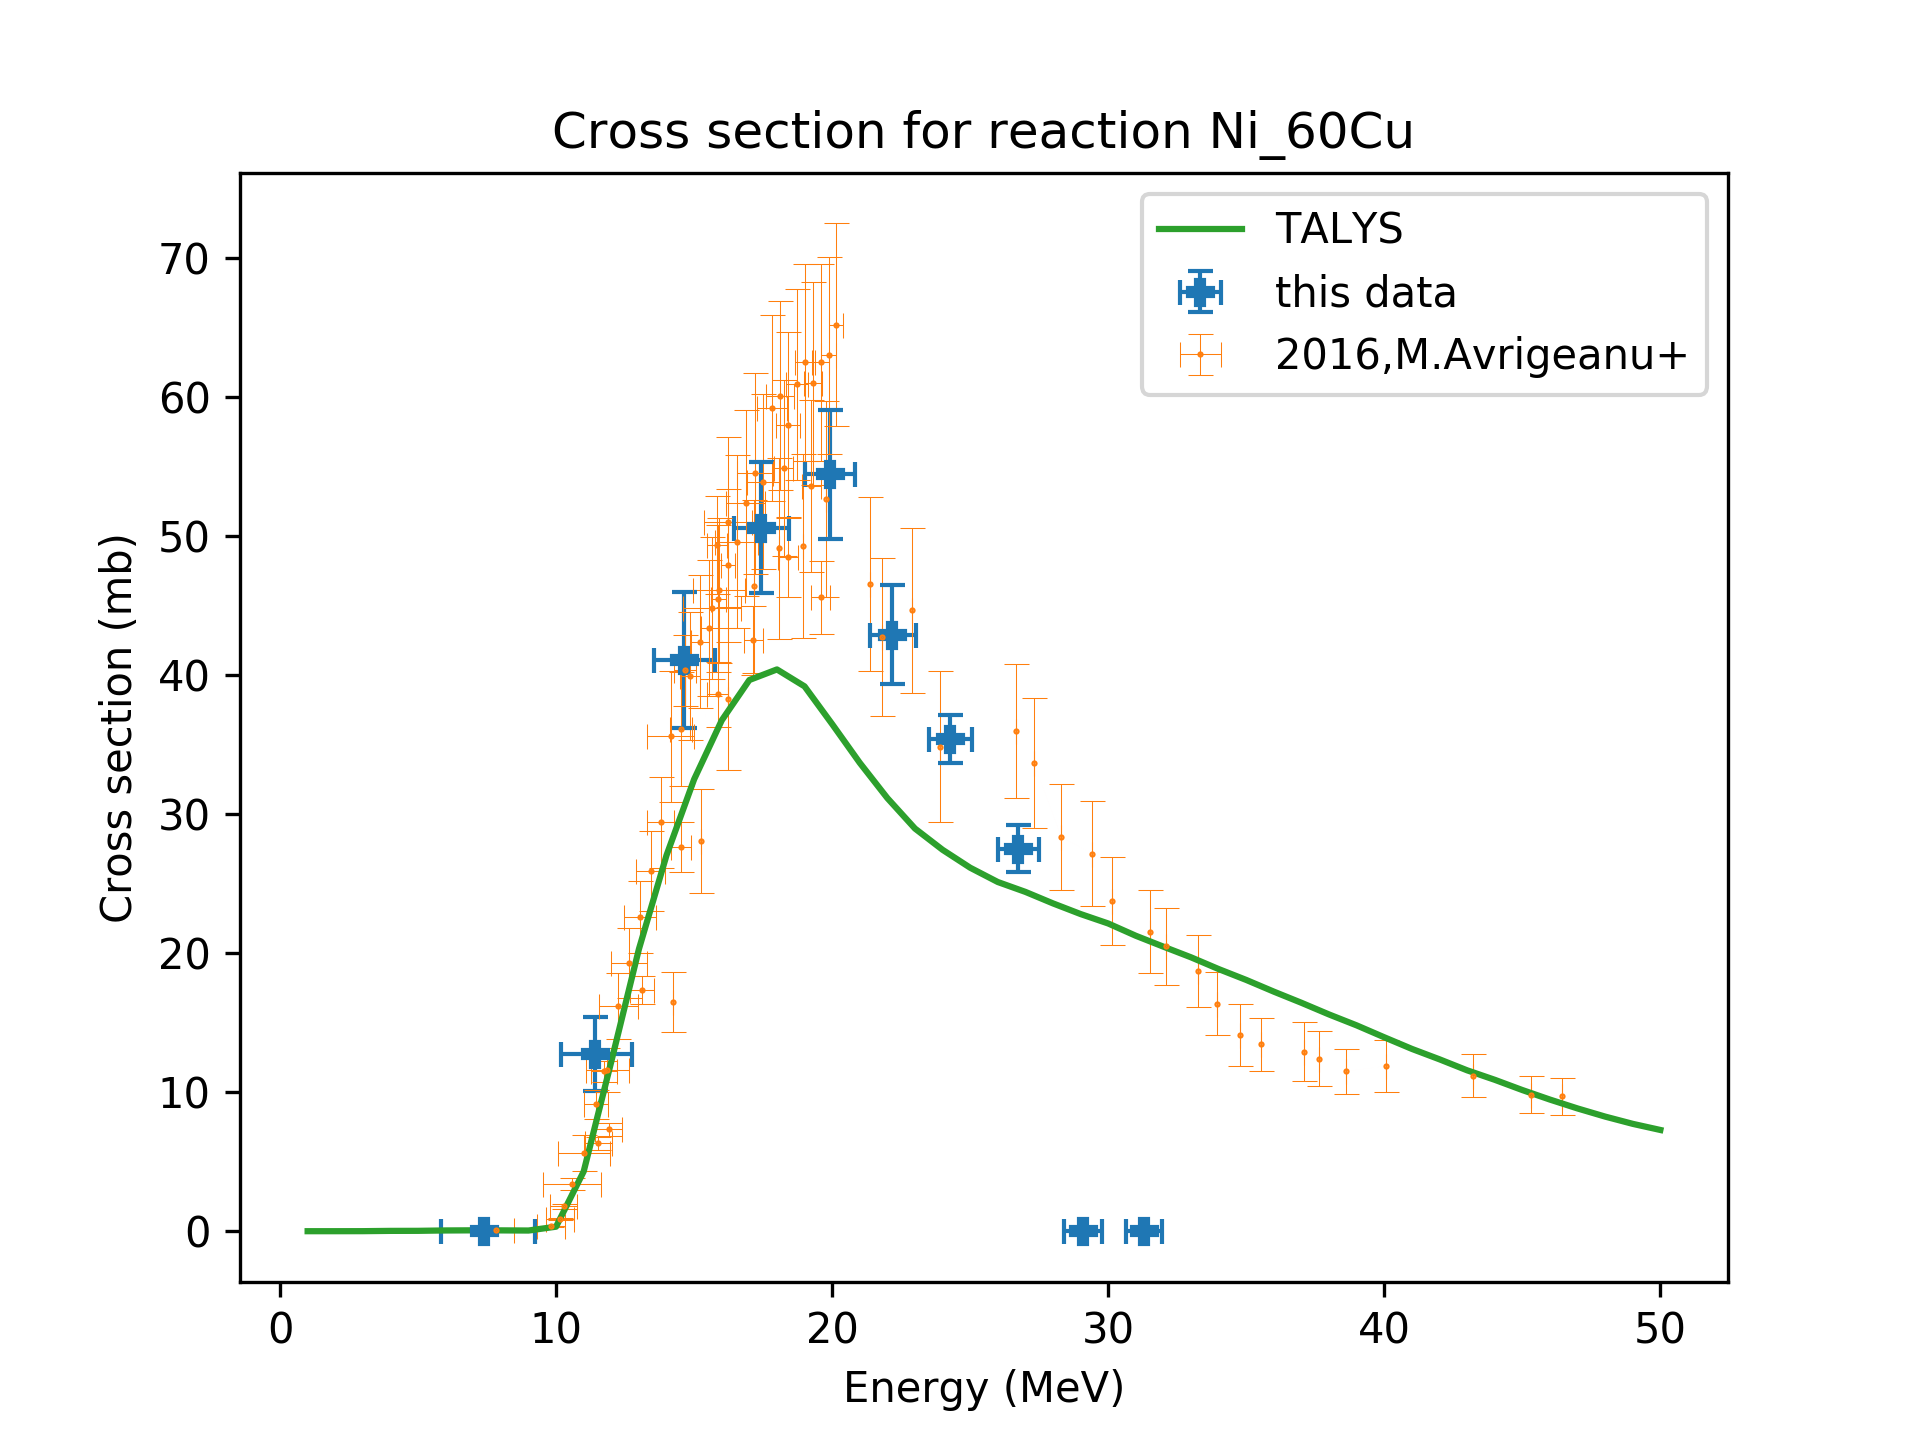
\includegraphics[width=5cm]{Results/Ni_60Cu.png} }}%
    \quad
    \subfloat[]{{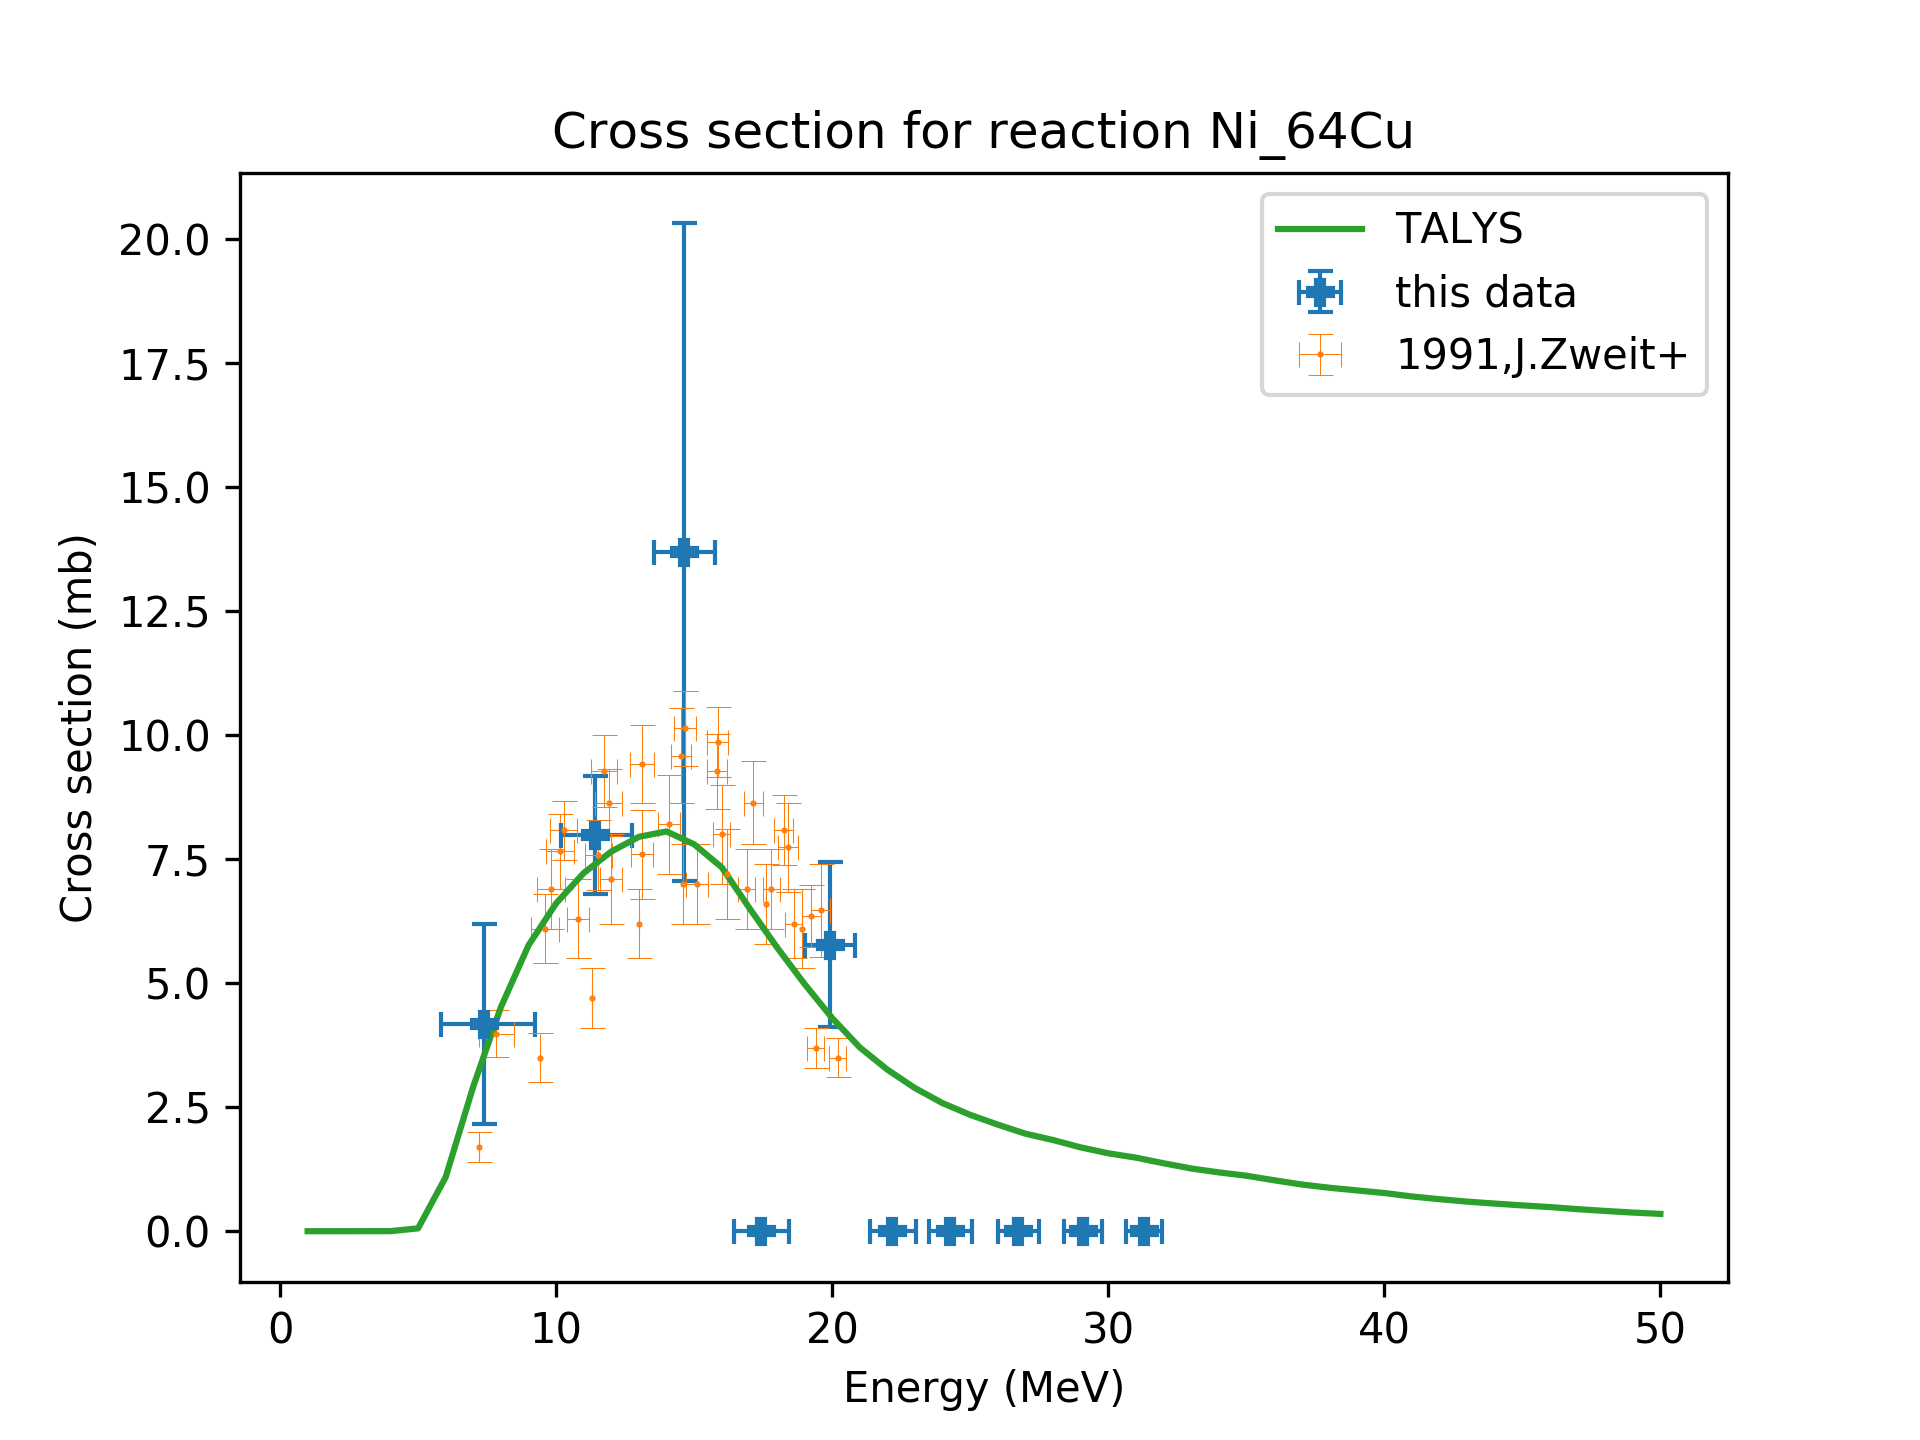
\includegraphics[width=5cm]{Results/Ni_64Cu.png} }}%
    \quad
    \subfloat[caption]{{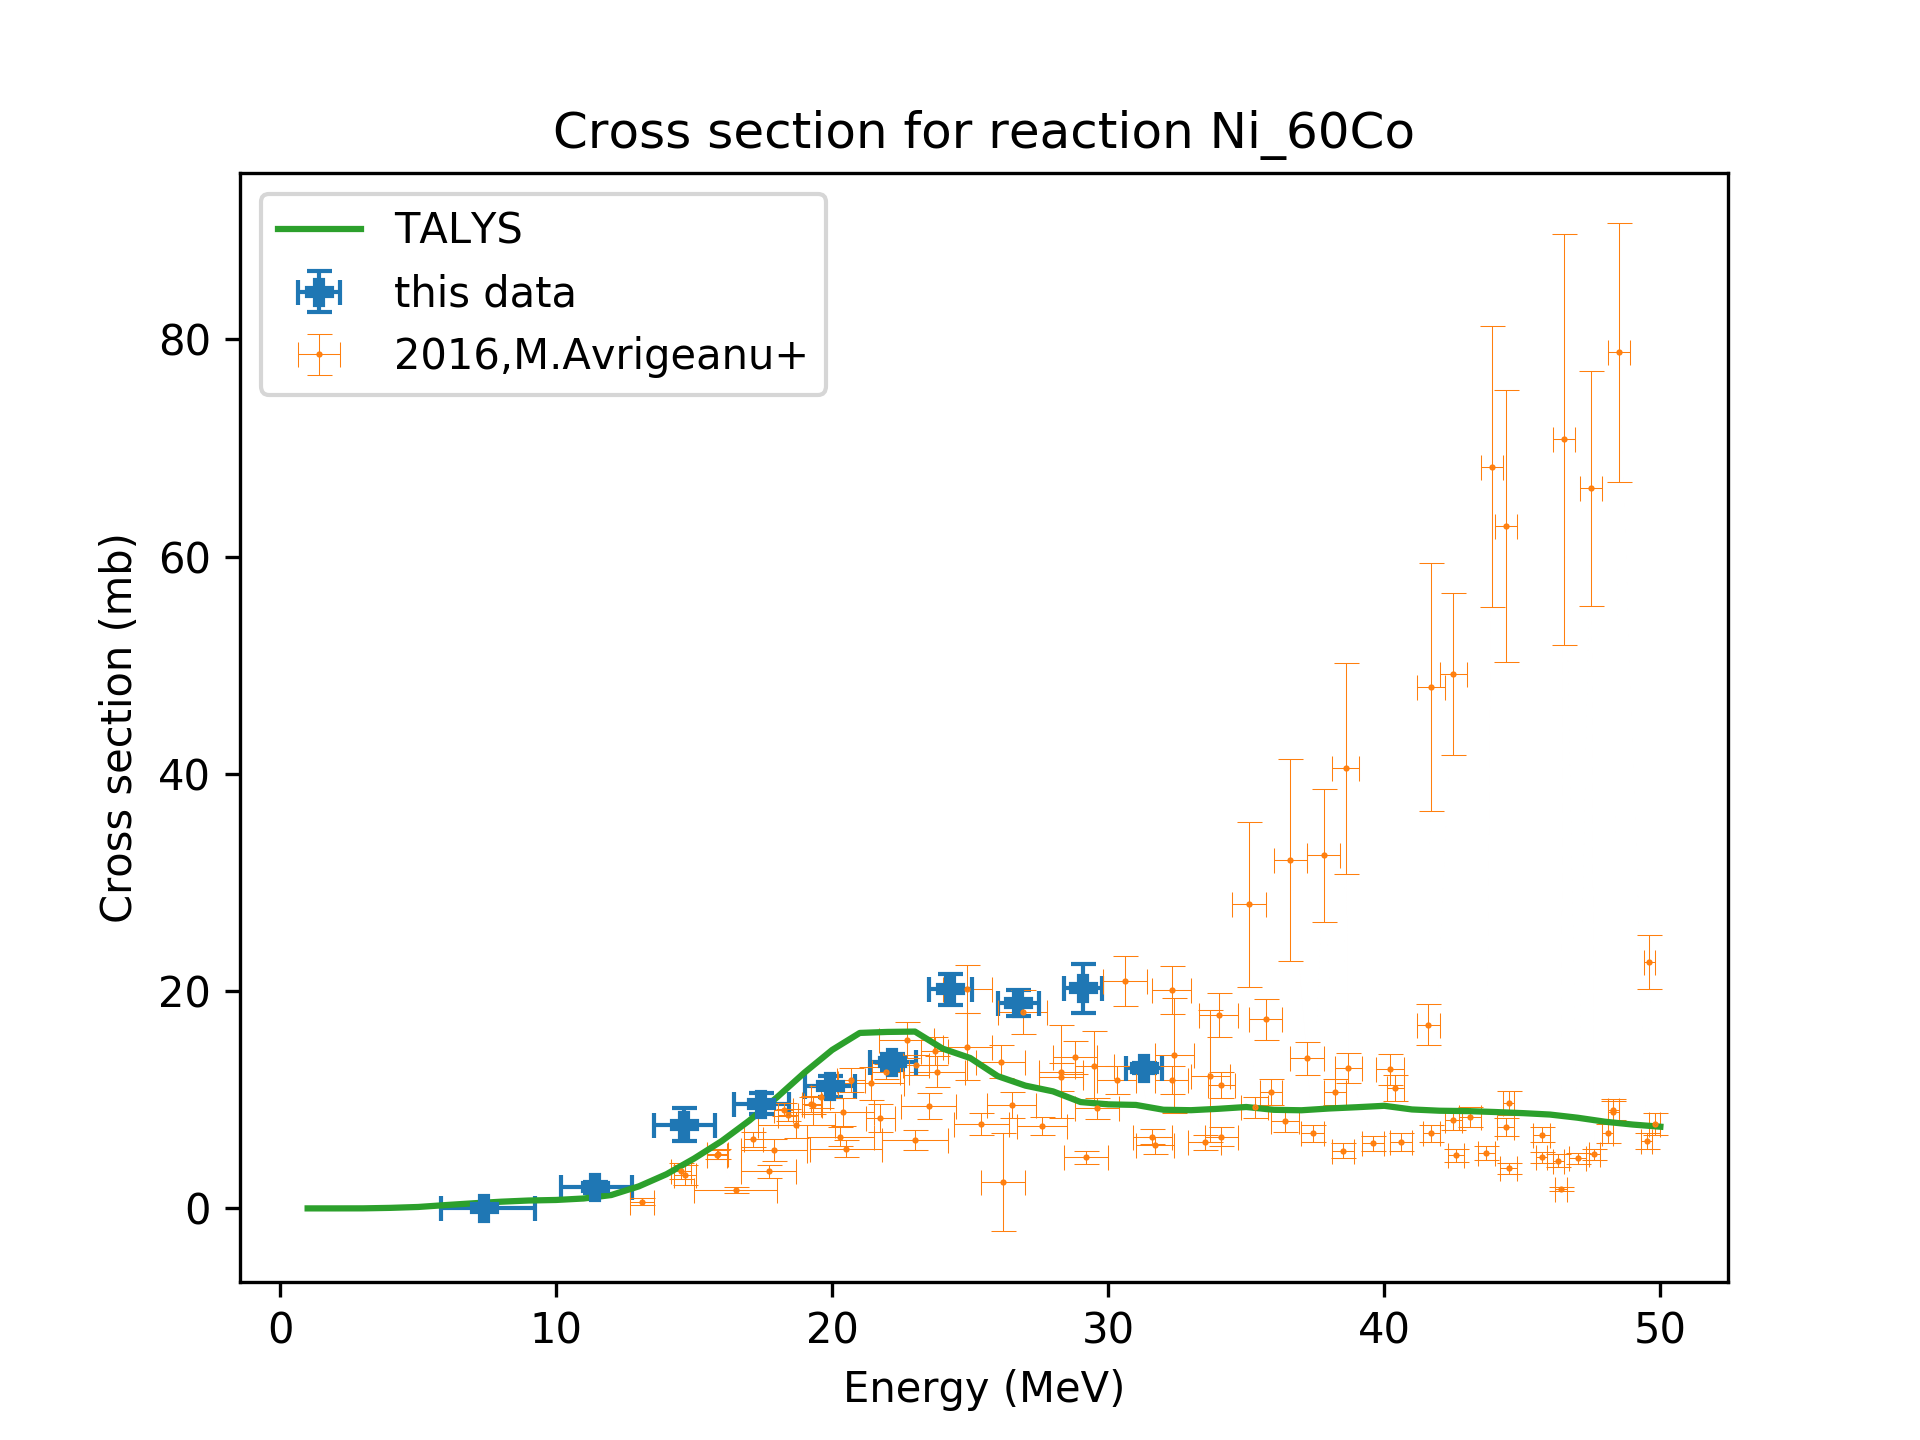
\includegraphics[width=5cm]{Results/Ni_60Co.png} }}%
    \quad
    \subfloat[]{{\includegraphics[width=5cm]{Results/Ni_65Ni.png} }}%
    \quad
    \subfloat[]{{\includegraphics[width=5cm]{Results/Ni_56Ni.png} }}%
    \quad
    \subfloat[]{{\includegraphics[width=5cm]{Results/Ni_55Co.png} }}%
    \quad
    \subfloat[]{{\includegraphics[width=5cm]{Results/Ni_56Mn.png} }}%
    \quad
    \subfloat[]{{\includegraphics[width=5cm]{Results/Ni_57Ni.png} }}%
    \quad
    \caption{Nickel  }%
    \label{fig:Ni_crosssections}%
\end{figure}

\section{Cupper cross sections}

\begin{figure}%
    \centering
    \subfloat[]{{\includegraphics[width=5cm]{Results/Cu_59Fe.png}}%
    \quad
    \subfloat[]{{\includegraphics[width=5cm]{Results/Cu_60Co.png} }}%
    \subfloat[]{{\includegraphics[width=5cm]{Results/Cu_61Co.png} }}%
    \quad
    \subfloat[]{{\includegraphics[width=5cm]{Results/Cu_61Cu.png} }}%
    \quad
    \subfloat[]{{\includegraphics[width=5cm]{Results/Cu_64Cu.png} }}%
    \quad
    \subfloat[caption]{{\includegraphics[width=5cm]{Results/Cu_65Ni.png} }}%
    \quad
    \caption{Cupper cross sections  }%
    \label{fig:Cu_crosssections}%
\end{figure}

\section{Iron cross sections}

\begin{figure}%
    \centering
    \subfloat[]{{\includegraphics[width=5cm]{Results/Fe_48V.png}}%
    \quad
    \subfloat[]{{\includegraphics[width=5cm]{Results/Fe_51Cr.png} }}%
    \subfloat[]{{\includegraphics[width=5cm]{Results/Fe_52Mn.png} }}%
    \quad
    \subfloat[]{{\includegraphics[width=5cm]{Results/Fe_53Fe.png} }}%
    \quad
    \subfloat[]{{\includegraphics[width=5cm]{Results/Fe_54Mn.png} }}%
    \quad
    \subfloat[caption]{{\includegraphics[width=5cm]{Results/Fe_55Co.png} }}%
    \quad
    \subfloat[caption]{{\includegraphics[width=5cm]{Results/Fe_57Co.png} }}%
    \quad
    \subfloat[caption]{{\includegraphics[width=5cm]{Results/Fe_58Co.png} }}%
    \quad
    \subfloat[caption]{{\includegraphics[width=5cm]{Results/Fe_59Fe.png} }}%
    \quad
    \caption{Iron cross sections  }%
    \label{fig:Fe_crosssections}%
\end{figure}


\chapter{Discussion}\label{Chapter:Discussion}
\noindent

Discussion on the different products, eg. iridium we expected more but it did not seem to be working the way we planned.. 


\section{Beamcurrent} 


\section{Iridium products}

To summarize, expected products from platinum and iridium were observed. However, there was no evidence of products from W, Ta, Re or Os. It is not said that we did not produce any isotopes of either, but there is not any reliable observation of the products. It seems like other reactions channels are favoured instead of alpha, or multiple proton emissions. For multiple cases, like $^{183}$Ta

\noindent \textcolor{blue}{The cross sections for the iridium products are listed in table \textcolor{red}{...}. Give a brief discussion on the varios products. And also, give a discussion of what we expected and what we did not see. THIS IS NOT A FINAL VERSION } In this experiment, $^{188}$Pt, $^{189}$Pt, $^{191}$Pt, $^{193m}$Pt, $^{188}$Ir, $^{189}$Ir, $^{190}$Ir, $^{192}$Ir, $^{194}$Ir, $^{194m2}$Ir, $^{188}$Re, $^{189}$Re and $^{190}$Re was observed. The products we did not observe was $^{183}$Ta (t$_{1/2}$=5.1 d), $^{186}$Re (t$_{1/2}$=3.7186 d), $^{186}$Ta (t$_{1/2}$=10.5 m), $^{18}$W (t$_{1/2}$=24.0 h). \\

\noindent $^{183}$Ta has a Q-value equal to 0.0 MeV for $^{191}$Ir(d,d$\alpha$)$^{183}$Ta and 4.020 MeV for $^{193}$Ir(d,nt2$\alpha$)$^{183}$Ta. The strongest gamma-line ($E_\gamma=59.318$ keV, $I_\gamma=42.1\%$) was not observed in any spectrum, and the second strongest gamma-line ($E_\gamma=246.059$ keV, $I_\gamma=27.2\%$) is within 1 keV from a gamma-line belonging to $^{189}$Ir ($E_\gamma=245.1$ keV, $I_\gamma=6.0\%$). Hence, we conclude that $^{183}$Ta was not observed. \\

\noindent $^{186}$Re has a Q-value equal to 0.0 MeV for $^{191}$Ir(d,t$\alpha$)$^{186}$Re and 13.1264 MeV for $^{193}$Ir(d,2nt$\alpha$)$^{183}$Ta. There is no data in the EXFOR database, and the reaction modelled cross sections provided by TALYS predicts that the cross section is \textcolor{red}{very low or zero} in this energy range. The two strongest gamma-lines were observed, ($E_\gamma=122.64$ keV, $I_\gamma=0.603\%$, $E_\gamma=137.157$ keV, $I_\gamma=9.47\%$). However, the activity which was estimated was not looking natural, hence the cross section curve is difficult to interpret \textcolor{red}{Might need some more work.} \\ 

\noindent $^{186}$Ta \\

\noindent $^{187}$W  \\

\noindent $^{188}$Pt has a Q-value equal to 19.593 MeV for $^{191}$Ir(d,4n)^$^{188}$Pt and 33.707 MeV $^{193}$Ir(d,6n). This decay is single step decay.  From experimental cross section data, the cross section is low up to about 37 MeV, and along with values provided from talys, the cross section measurements were expected to be low. However, we are confident that we have a measurement at .... 

\noindent 


\chapter{Conclusion and future aspects}\label{Chapter:Conclusion}
\noindent









\appendix 

\chapter{Statistics} \label{ch_app:statistics}

\noindent \textcolor{red}{Uncertainty in statistics refers to the standard deviation of the data, which gives a number of the spreading of the data from the mean value of the data \textcolor{red}{citation}. The variance is the standard deviation squared, which weights the variables to a higher degree. }

\begin{equation}
    std = \sqrt{\sigma^2}
\end{equation}

\begin{equation}
    \sigma = \sqrt{\frac{1}{N}\sum_{i=1}^N (x_i - \overline{x})^2}
\end{equation}
\noindent
where N is the number of measurements, $x_i$ is a measurement and $\overline{x}$ is the average over all measurements. 


\noindent 
A function $f$ with input $x$ and a set of variables $\vec{\beta}= \beta_1, \beta_2, ..., \beta_n$ and output y can be written on the following form
\begin{equation}
    y = f(x, \vec{\beta})
\end{equation}

\noindent The uncertainty in y is dependent on the uncertainty in the different input variables $ \vec{\beta}$. The matrix expression for error propagation is (Tellinghuisen, Joel, Statistical error propagation)\footnote{A full derivation of the expression can be found in Uncertainty Propagation for Measurements with multiple output quantities, Dobbert, Schrijver}
\begin{equation} \label{eq:variance_full}
    \sigma^2_y = \mathbf{J}\cdot \mathbf{V}\cdot \mathbf{J}^T 
\end{equation} 

\noindent where $\sigma^2_y$ is the variance in y, J is the Jacobian matrix
\begin{equation}
\mathbf{J} = 
    \begin{bmatrix}
       \frac{\partial f}{\partial \beta_1} &  \frac{\partial f}{\partial \beta_2} & \cdots & \frac{ \partial f}{\partial \beta_n}
    \end{bmatrix}
\end{equation}

\noindent and V is the variance-covariance matrix 

\begin{equation}
\mathbf{V} = 
\begin{bmatrix}
  \sigma_0^2 & \sigma_{0,1} & \cdots & \sigma_{0,n} \\
  \sigma_{1,0} & \sigma_{1}^2 & \cdots & \sigma_{1,n} \\
  \vdots  & \vdots  & \ddots & \vdots  \\
  \sigma_{n,0} & \sigma_{n,1} & \cdots & \sigma_{n}^2
 \end{bmatrix}
\end{equation}


\noindent In the cases where the input parameters are uncorrelated, all non-diagonal elements in the variance-covariance matrix is equal to zero, and the expression for the variance is simplified to 

\begin{equation} \label{eq:variance_simplified}
    \sigma_y^2 = \sum_{i=1}^n \Big(\frac{\partial f}{\partial \beta_i } \Big)^2 \sigma_{\beta_i}^2
\end{equation}

\noindent Whenever the input parameters are correlated, which means that $\sigma_{\beta_i, \beta_j}\neq 0$, we have to apply equation \ref{eq:variance_full}, otherwise, the simplification in equation \ref{eq:variance_simplified} will give wrong error propagation. \\

\noindent To evaluate the partial derivatives of f, the computational derivation is applicable

\begin{equation}
    \frac{\partial f}{\partial \beta_i} \simeq\frac{f(x, \beta_i + \frac{\Delta \beta_i}{2}) - f(x, \beta_i-\frac{\Delta \beta_i}{2})}{\Delta \beta_i}
\end{equation}

\noindent where $\Delta\beta_i$ is a small number, like $10^{-8}\beta_i$. \\


\noindent 
For a function $f=xy $, the variance can be expressed from equation \ref{eq:variance_full}, where  $$\mathbf{J}=\begin{bmatrix}y & x \end{bmatrix}$$ and $$\mathbf{V}=\begin{bmatrix} \sigma_x^2 & \sigma_{x,y}\\\sigma_{y,x} & \sigma_{y^2} \end{bmatrix}$$ 

\begin{equation}
    \sigma_f^2 = x^2\sigma_y^2 + y^2\sigma_x^2 + 2 xy \sigma_{x,y}
\end{equation}

\noindent If we multiply each term so that we can collect $f^2$ in the numerator, the variance in f can be expressed as 

\begin{equation}
    \sigma_f^2 = f^2 \big( \frac{\sigma_x^2}{x^2} + \frac{\sigma_y^2}{y^2} + \frac{2\sigma_{x,y}}{xy} \Big)
\end{equation}

\noindent if the variables x and y are uncorrelated, the variance is further simplified, and more terms can be included easily. The simplified standard deviation of a function $f(\vec{\beta})=\beta_1 \cdot \beta_2 \cdots \beta_n $ with uncorrelated variables is thus
\begin{equation} \label{eq:uncertainty_simplification}
    \sigma_f = |f|\sqrt{ \Big( \frac{\sigma_{\beta_1}}{\beta_1}\Big)^2 +  \Big( \frac{\sigma_{\beta_2}}{\beta_2}\Big)^2 + \cdots  \Big( \frac{\sigma_{\beta_n}}{\beta_n}\Big)^2    } 
\end{equation}



\chapter{Tabulated information for each product nuclide}

\chapter{Tables} \label{ch:tables}

Tables \ref{tab:Products_information_FE}, \ref{tab:Products_information_NI}, \ref{tab:Products_information_CU} and \ref{tab:Products_information_IR} containts information regarding products nuclei from iron, nickel, copper and iridium (respectively). The tables contains values such as energy level, half-life, decay mode, production route with the lowest Q value within the energy range of the deuterons. To estimate other production routes, table \ref{tab:decaychannel_particles} provides information on how much to increase the Q value to the desired decaychannel.  Along with the gamma-lines and intensities that were used in the analysis, the tables contain information which is used to describe the excitation function for each product nuclei. 

\begin{table}[]
    \centering
    \caption{The table shows the most common decay channels for the decay routes available in this energy region. $\Delta$ is the binding energy of the alpha particle, which can be calculated using equation \ref{eq:Binding_energy1}, where the mass of the proton is $m_p = 938.28$ MeV/c$^2$ and $m_n=939.57$ MeV/c$^2$. $\Delta$ is thus the difference in in energy-mass between the particle composed of protons and or neutrons, and a equal number of protons and neutrons independent. All parities are positive due to angular momentum $\ell=0$.  }
    \begin{tabular}{|c|c|c|c|c|}
         \hline 
         Particle & \Delta (MeV) &J^\pi & Charge \\
         \hline
         p & - & $\frac{1}{2}^+$ & +1 \\
         n & - & $\frac{1}{2}^+$ & 0 \\
         d & 2.2 & $1^+$ & +1 \\
         t & 8.5 & $\frac{1}{2}^+$ & +1 \\
         ^{3}He & 7.7 & $\frac{1}{2}^+$ & +2 \\
        \alpha & 28.3 & 0^+ & +2 \\
        \hline
    \end{tabular}
    \label{tab:decaychannel_particles}
\end{table}

%\usepackage{longtable}
%\usepackage{tabu, booktabs}

\newpage

\centering
    \begin{longtable}{ccc|cc|cc}
    \caption{Products observed on Iron foils. Iron four five stable isotopes: $^{54}$Fe (5.845\%), $^{56}$Fe (91.754 \%), $^{57}$Fe (2.119\%) and  $^{58}$Fe (0.282\%). If the nucleus has provided energy level, the nucleus is an isomer, if nothing then ground state. \textcolor{red}{The table is inspired by Tarkanyi et al 2019 (ir paper))} } 
    %\begin{tabular}{|c|c|c|cc|cc|}
        \hline
        \thead{\textbf{Nuclide}\\ \textbf{level (keV)}} & \thead{\textbf{Half life}} & \thead{\textbf{Decay mode}} & \thead{\textbf{Reaction route}} & \thead{\textbf{Q value (keV)}} & \thead{$\mathbf{E_\gamma}$ \textbf{(keV)}} & \thead{$\mathbf{I_\gamma}$ \textbf{(\%)}}  \\
        \hline
        \makecell[t]{$^{48}$V \\$\quad$(0.0)} & \makecell[t]{15.9735 d} & \makecell[t]{\epsilon:100\%} & \makecell[t]{$^{54}$Fe(d,2$\alpha$) \\ $^{56}$Fe(d,2n2$\alpha$) \\ $^{57}$Fe(d,3n2$\alpha$)} & \makecell[t]{-3490.9 \\ -23986.1} & \makecell[t]{944.130 \\ 983.525 \\ 1312.106} & \makecell[t]{7.870 \\ 99.98\\98.2} \hline
        
        \makecell[t]{$^{51}$Cr\\$\quad$(0.0) } & \makecell[t]{27.704 d} & \makecell[t]{\epsilon:100\%} & \makecell[t]{$^{54}$Fe(d,d$^3$He) \\ $^{56}$Fe(d,t$\alpha$) \\ $^{57}$Fe(d,nt$\alpha$) \\ $^{58}$Fe(d,2nt$\alpha$) } & \makecell[t]{-19734.3 \\ -13394 \\ -21040.8 \\ -31085.4} & \makecell[t]{320.0824} & \makecell[t]{9.910} \\ \hline
        
        \makecell[t]{$^{52}$Mn\\$\quad$(0.0)} & \makecell[t]{5.591 d d} & \makecell[t]{\epsilon: 100\%} & \makecell[t]{$^{54}$Fe(d,$\alpha$) \\ $^{56}$Fe(d,2n$\alpha$) \\ $^{57}$Fe(d,3n$\alpha$)} & \makecell[t]{5163.6 \\ -15331.6 \\ -22977.7 } & \makecell[t]{346.02 \\ 744.233 \\ 848.18 \\ 935.544 \\ 1246.278 \\ 1333.649 \\ 1434.092} & \makecell[t]{0.980 \\ 90.0 \\ 3.32 \\ 94.5 \\ 4.21 \\ 5.07 \\ 100.0 } \\ \hline        
        \makecell[t]{$^{54}$Mn\\$\quad$(0.0)} & \makecell[t]{312.20 d} & \makecell[t]{\epsilon:100\%} & \makecell[t]{$^{54}$Fe(d,2p) \\ $^{56}$Fe(d,$\alpha$) \\ $^{57}$Fe(d,n$\alpha$) \\ $^{58}$Fe(d,2n$\alpha$)} & \makecell[t]{-2139.1 \\ 5661.4 \\ -1984.7 \\ -12029.3} & \makecell[t]{834.8480} & \makecell[t]{99.9760} \\ \hline
        
        \makecell[t]{$^{53}$Fe\\$\quad$(0.0)} & \makecell[t]{8.51 m ????} & \makecell[t]{\epsilon:100\%} & \makecell[t]{$^{54}$Fe(d,t) \\$^{56}$Fe(d,2nt) } & \makecell[t]{-7121.1 \\  -27616.3} & \makecell[t]{377.9} & \makecell[t]{42\%} \\ \hline
        
        \makecell[t]{$^{59}$Fe\\$\quad$(0.0)} & \makecell[t]{44.490 d} & \makecell[t]{\beta^-: 100\%} & \makecell[t]{$^{58}$Fe(d,p)} & \makecell[t]{4356.44} & \makecell[t]{1099.245 \\ 1291.590} & \makecell[t]{56.5\\43.2} \\ \hline
        
        \makecell[t]{$^{55}$Co\\$\quad$(0.0)} & \makecell[t]{17.53 h} & \makecell[t]{\epsilon:100\%} & \makecell[t]{$^{54}$Fe(d,n) \\ $^{56}$Fe(d,3n) \\ $^{57}$Fe(d,4n)} & \makecell[t]{2839.8 \\ -17655.4 \\ -25301.5} & \makecell[t]{91.9 \\ 477.2 \\ 803.7 \\827.0\\ 931.1 \\ 1316.6 \\ 1370.0 \\ 1408.5  \\ 2177.6 \\ 2872.4 \\ 2938.9 } & \makecell[t]{1.16 \\ 20.2 \\ 1.87 \\ 0.21 \\ 75\\ 7.1 \\ 2.9 \\ 16.9 \\ 0.29 \\ 0.118 \\ 0.057 } \\ \hline
        
        \makecell[t]{$^{56}$Co\\$\quad$(0.0)} & \makecell[t]{77.236 d} & \makecell[t]{\epsilon:100\%} & \makecell[t]{$^{56}$Fe(d,2n)\\$^{57}$Fe(d,3n) \\$^{58}$Fe(d,4n) } & \makecell[t]{-7573 \\ -15219.7 \\ -25264.3 } & \makecell[t]{263.434 \\ 486.55 \\ 733.514 \\ 787.743 \\ 846.770 \\ 852.732 \\ 896.510 \\ 977.372 \\ 996.948 \\ 1037.843 \\ 1140.368 \\ 1159.944 \\ 1175.101 \\ 1198.888 \\ 1238.288 \\ 1335.40 \\ 1360.212 \\ 1771.357 \\ 1963.741 \\ 2015.215 \\ 2034.791 \\ 2212.944 \\ 2276.131 \\ 2598.500} & \makecell[t]{0.0220 \\ 0.0540 \\ 0.191 \\ 0.311 \\ 99.9399 \\ 0.049 \\ 0.073 \\ 1.421 \\ 0.111 \\ 14.05 \\ 0.132 \\ 0.094 \\2.252 \\ 0.049 \\ 66.46 \\ 0.1224 \\ 4.283 \\ 15.41 \\ 0.707 \\ 3.016\\ 7.77 \\ 0.388 \\ 0.118 \\ 16.97 } \\ \hline
        
        \makecell[t]{$^{57}$Co\\$\quad$(0.0)} & \makecell[t]{271.74 d} & \makecell[t]{\epsilon: 100\%} & \makecell[t]{$^{56}$Fe(d,n) \\ $^{57}$Fe(d,2n \\ $^{58}$Fe(d,3n)} & \makecell[t]{3802.9 \\ -3843.2 \\ -13887.8 } & \makecell[t]{122.06065 \\ 136.47356} & \makecell[t]{85.60 \\ 10.68 } \\ \hline
        
        \makecell[t]{$^{58}$Co\\$\quad$(0.0)} & \makecell[t]{70.86} & \makecell[t]{\epsilon:100\%} & \makecell[t]{$^{57}$Fe(d,n) \\ $^{58}$Fe(d,2n)} & \makecell[t]{4729.7 \\ -5314.9} & \makecell[t]{810.7593} & \makecell[t]{99.450} \\ \hline 
        
        %\makecell[t]{\\$\quad$(0.0)} & \makecell[t]{} & \makecell[t]{} & \makecell[t]{} & \makecell[t]{} & \makecell[t]{} & \makecell[t]{} \\ \hline
        
        
        
    %\end{tabular}
    \label{tab:Products_information_FE}
    \end{longtable}
%\end{table}

%\begin{table}
    \centering
    \begin{longtable}{ccc|cc|cc}
    \caption{Products observed on Nickel foils. Nickel has five stable isotopes: $^{58}$Ni (68.077\%), $^{60}$Ni (26.223 \%), $^{61}$Ni (1.1399\%), $^{62}$Ni (3.6346\%) and $^{64}$Ni (0.9255\%). If the nucleus has provided energy level, the nucleus is an isomer, if nothing then ground state. \textcolor{red}{The table is inspired by Tarkanyi et al 2019 (ir paper))} } 
    %\begin{tabular}{|c|c|c|cc|cc|}
        \hline
        \thead{\textbf{Nuclide}\\ \textbf{level (keV)}} & \thead{\textbf{Half life}} & \thead{\textbf{Decay mode}} & \thead{\textbf{Reaction route}} & \thead{\textbf{Q value (keV)}} & \thead{$\mathbf{E_\gamma}$ \textbf{(keV)}} & \thead{$\mathbf{I_\gamma}$ \textbf{(\%)}}  \\
        \hline
        \makecell[t]{$^{52}$Mn\\ $\quad$(0.0) } &\makecell[t]{5.591 d \\ 21.1 m} & \makecell[t]{$\epsilon: 100\% $} & \makecell[t]{$^{58}$Ni(d,2$\alpha$) \\ $^{60}$Ni(d,2n2$\alpha$ \\ $^{61}$Ni(d,3n2$\alpha$)}   & \makecell[t]{-1235.6 \\ -21622.6 \\ -29442.7} & \makecell[t]{744.233 \\ 935.544 \\ 1246.278 \\ 1434.092} & \makecell[t]{90.0 \\ 94.5\\4.21 \\100.0} \\
        %\makecell{$^{52m}$Mn \\ $\quad$(377.7495)} & 21.1 m & \makecell{\epsilon: 98.22\% \\ IT: 1.78\% } & & & & \\ 
        \hline

        \makecell[t]{$^{54}$Mn \\ $\quad$(0.0) } & \makecell[t]{312.20 d} & \makecell[t]{\epsilon:100\%} & \makecell[t]{$^{58}$Ni(d,2p$\alpha$) \\ $^{60}$Ni(d,2$\alpha$) \\  $^{61}$Ni(d,n2$\alpha$) \\ $^{62}$Ni(d,2n2$\alpha$)} & \makecell[t]{ -8538.3 \\ -629.6 \\ -8449.7 \\ -19045.4 }& 834.848 & 99.9760 \\
        \hline 
        
        \makecell[t]{$^{59}$Fe\\ $\quad$(0.0)} & \makecell[t]{44.490 d} & \makecell[t]{\beta^-: 100\%} & \makecell[t]{$^{60}$Ni(d,3p) \\ $^{61}$Ni(d,p$^3$He) \\ $^{62}$Ni(d,p$\alpha$) \\ $^{64}$Ni(d,t$\alpha$) } & \makecell[t]{-12539.5 \\ -12641.6 \\ -2659.7 \\ -10673.1}   & 1291.590 & 43.2 \\
        \hline
        
        \makecell[t]{$^{55}$Co\\ $\quad$(0.0)} & \makecell[t]{17.53 h} & \makecell[t]{\epsilon: 100\% } & \makecell[t]{$^{58}$Ni(d,n$\alpha$) \\ $^{60}$Ni(d,3n$\alpha$) \\ $^{61}$Ni(d,4n$\alpha$) } & \makecell[t]{-3559.4 \\ -23946.4 \\ -31766.5} & \makecell[t]{91.9 \\ 385.4 \\ 477.2 \\ 520.0 \\ 803.7 \\ 827.0 \\ 931.1 \\ 984.6 \\1212.8 \\ 1316.6 \\ 1370.0 \\ 1408.5 \\ 1792.1 \\ 2177.6 \\ 2872.4 } & \makecell[t]{1.16\\0.54 \\ 20.2 \\ 0.83 \\ 1.87 \\ 0.21 \\ 75 \\ 0.52 \\ 0.26 \\ 7.1 \\ 2.9 \\ 16.9 \\ 0.082 \\ 0.29 \\ 0.118} \\
        \hline
        
        \makecell[t]{$^{56}$Co \\ $\quad$(0.0)} & \makecell[t]{77.236 d} & \makecell[t]{\epsilon:100\%} & \makecell[t]{$^{58}$Ni(d,$\alpha$) \\ $^{61}$Ni(d,2n$\alpha$) \\ $^{61}$Ni(d,3n$\alpha$) \\$^{62}$Ni(d,4n$\alpha$)} & \makecell[t]{6522.5 \\ -13864.5 \\ -21684.6 \\ -32280.4} & \makecell[t]{787.743 \\846.770\\ 977.372 \\ 1175.101 \\ 1963.741 \\ 2015.215 \\ 2034.791} & \makecell[t]{0.3111 \\ 99.9399 \\ 1.421 \\ 2.252 \\ 0.707 \\ 3.016 \\ 7.77}\\ 
        \hline
        
       \makecell[t]{$^{58}$Co \\ $\quad$(0.0) } & \makecell[t]{70.86 d} & \makecell[t]{\epsilon:100\%} & \makecell[t]{$^{58}$Ni(d,2n) \\ $^{60}$Ni(d,$\alpha$) \\ $^{61}$Ni(d,n$\alpha$) \\ $^{62}$Ni(d,2n$\alpha$) \\ $^{64}$Ni(d,4n$\alpha$)}  & \makecell[t]{-1823.8 \\ 6084.9 \\-1735.3 \\-12331.0\\ -28826.2}   & \makecell[t]{810.7593\\ 863.951 \\1674.725 } & \makecell[t]{99.450 \\ 0.686 \\ 0.517}\\
        %\makecell{$^{58m}$Co \\ $\quad$(24.88921) } & \makecell{70.86 d} & \makecell{IT:100\%} & & & & \\ 
        \hline
        
        \makecell[t]{$^{60}$Co \\ $\quad$(0.0)} & \makecell[t]{1925.28 d} & \makecell[t]{$\beta^-$: 100\%} & \makecell[t]{$^{60}$Ni(d,2p)  \\ $^{61}$Ni(d,$^3$He) \\ $^{62}$Ni(d,$\alpha$) \\ $^{64}$Ni(d,2n$\alpha$)}  & \makecell[t]{-4265.0 \\ -4367.09 \\ 5614.8 \\ -10880.4 } &\makecell[t]{1173.228 \\ 1332.492} & \makecell[t]{99.85 \\ 99.9826} \\
        \hline
        
        \makecell[t]{$^{56}$Ni\\$\quad$(0.0)} & \makecell[t]{6.075 d} & \makecell[t]{\epsilon: 100\%} & \makecell[t]{$^{58}$Ni(d,nt)} & \makecell[t]{-16206.6} & \makecell[t]{158.38 \\ 480.44 \\ 749.95 \\ 811.85 \\ 1561.80} & \makecell[t]{98.8 \\ 36.5 \\ 49.5 \\ 86.0 \\ 14.0 } \\ 
        \hline 
        
        
        
        \makecell[t]{$^{57}$Ni\\ $\quad$(0.0)} & \makecell[t]{35.60 h} & \makecell[t]{\beta^+: 100\%} & \makecell[t]{$^{58}$Ni(d,t) \\ $^{60}$Ni(d,2nt)} & \makecell[t]{-5959.0 \\ -26346.0} & \makecell[t]{ 379.94 \\ 673.44 \\ 906.98 \\ 1046.68 \\ 1224.00 \\ 1377.63 \\ 1730.44 \\ 1757.55 \\ 1897.42 \\ 1919.52 \\ 2133.04 \\ 2804.20 \\ } & \makecell[t]{0.0670 \\ 0.0491 \\ 0.0613 \\ 0.134 \\ 0.063 \\ 81.7 \\ 0.052 \\ 5.75 \\ 0.028 \\ 12.3 \\ 0.0286 \\ 0.098 } \\
        \hline
         
         \makecell[t]{$^{65}$Ni \\ $\quad$(0.0)} & \makecell[t]{2.51719 h} & \makecell[t]{\beta^-: 100\% } & \makecell[t]{$^{64}$Ni(d,p)} & \makecell[t]{3873.51} &  \makecell[t]{366.27 \\ 1481.84 \\ 1623.42 \\ 1724.92} & \makecell[t]{4.81 \\ 23.59 \\ 0.498 \\ 0.399 } \\
         \hline
         
         \makecell[t]{$^{60}$Cu\\ $\quad$(0.0)} & \makecell[t]{23.7 m } & \makecell[t]{\epsilon: 100\%} & \makecell[t]{$^{60}$Ni(d,2n) \\ $^{61}$Ni(2,3n) \\ $^{62}$Ni(d,4n) } & \makecell[t]{-9134.9 \\ -16955.0 \\ -27550.7 } & \makecell[t]{467.3 \\ 497.9 \\ 643.2 \\ 952.4 \\ 1035.2 \\ 1110.5 \\ 1293.7 \\ 1791.6 \\ 1861.6 \\ 1936.9 \\ 2061.0 \\ 2158.9 \\ 2403.3 \\ 2687.9 \\ 2746.1} & \makecell[t]{3.52 \\ 1.67 \\ 0.97 \\ 2.73 \\3.70 \\ 1.06\\ 1.85 \\ 45.4 \\ 4.8 \\ 2.20 \\ 0.79 \\ 3.34 \\ 0.77 \\ 0.44 \\ 1.06}    \\
         \hline
         
         \makecell[t]{$^{61}$Cu} & \makecell[t]{3.339 h} & \makecell{\epsilon:100\%} & \makecell[t]{$^{60}$Ni(d,n) \\ $^{61}$Ni(d,2n) \\ $^{62}$Ni(d,3n) \\ $^{64}$Ni(d,5n)} & \makecell[t]{2575.3 \\ -5244.8 \\ -15840.5 \\ -32335.7 } & \makecell[t]{282.956 \\ 373.050 \\ 529.169\\ 588.605 \\ 625.605 \\ 656.008 \\ 816.692 \\ 841.211 \\ 902.294 \\ 1032.162 \\ 1073.465 \\ 1132.351 \\ 1185.234 \\ 1446.492} & \makecell[t]{12.2 \\ 2.1 \\ 0.38 \\ 1.17 \\ 0.040 \\ 10.8 \\ 0.31 \\ 0.21 \\ 0.083 \\ 0.043 \\ 0.033 \\ 0.090 \\ 3.7 \\ 0.045} \\ 
         \hline
        
        \makecell[t]{$^{64}$Cu} & \makecell[t]{12.701 h} & \makecell[t]{\epsilon:100\% \\ \beta^-:38.5\%} & \makecell[t]{$^{64}$Ni(d,2n)} & \makecell[t]{-4681.3} & \makecell[t]{1345.77} & \makecell[t]{0.475}   \\
        \hline
         %\thead{$^{52m}$Mn \\ (377.7495)} &\makecell{5.591 d} & \makecell{$\epsilon: 100\% $} & $^{58}$Ni(d,2$\alpha$)$^{52}$Mn & -1235.6 & 1278.5 &         
    %\end{tabular}
    \label{tab:Products_information_NI}
    \end{longtable}
%\end{table}





\newpage
\centering
    \begin{longtable}{ccc|cc|cc}
    \caption{Products observed on Cupper foils. Cupper has two stable isotopes: $^{63}$Cu (69.15\%) and $^{65}$Cu (30.85 \%).If the nucleus has provided energy level, the nucleus is an isomer, if nothing then ground state. \textcolor{red}{The table is inspired by Tarkanyi et al 2019 (ir paper))} } 
    %\begin{tabular}{|c|c|c|cc|cc|}
        \hline
        \thead{\textbf{Nuclide}\\ \textbf{level (keV)}} & \thead{\textbf{Half life}} & \thead{\textbf{Decay mode}} & \thead{\textbf{Reaction route}} & \thead{\textbf{Q value (keV)}} & \thead{$\mathbf{E_\gamma}$ \textbf{(keV)}} & \thead{$\mathbf{I_\gamma}$ \textbf{(\%)}}  \\
        \hline
        
        \makecell[t]{$^{59}$Fe\\$\quad$(0.0)} & \makecell[t]{44.490 d} & \makecell[t]{\beta^-: 100\%} & \makecell[t]{$^{63}$Cu(d,2p$\alpha$) \\ $^{65}$Cu(d,2$\alpha$)} & \makecell[t]{-8782.1 \\ 1687.0} & \makecell[t]{1099.245 \\ 1291.590} & \makecell[t]{56.5 \\43.2 } \\ \hline
        
        \makecell[t]{$^{60}$Co\\$\quad$(0.0)} & \makecell[t]{1925.28 d} & \makecell[t]{\beta^-:100\%} & \makecell[t]{$^{63}$Cu(d,p$\alpha$) \\ $^{65}$Cu(d,t$\alpha$)} & \makecell[t]{-507.6 \\ -9852.4} & \makecell[t]{1173.228 \\ 1332.492} & \makecell[t]{99.85 \\ 99.9826 } \\ \hline
        
        \makecell[t]{$^{61}$Co\\$\quad$(0.0)} & \makecell[t]{1.649 h} & \makecell[t]{\beta^-:100\%} & \makecell[t]{$^{63}$Cu(d,p$^3$He) \\ $^{65}$Cu(d,d$\alpha$)} & \makecell[t]{-11766.2 \\ -9015.1 } & \makecell[t]{67.412} & \makecell[t]{84.7} \\ \hline
        
        \makecell[t]{$^{65}$Ni\\$\quad$(0.0)} & \makecell[t]{2.51719 h} & \makecell[t]{\beta^-:100\%} & \makecell[t]{$^{65}$Cu(d,2p)} & \makecell[t]{-3580.2} & \makecell[t]{1481.84} & \makecell[t]{23.59} \\ \hline
        
        \makecell[t]{$^{61}$Cu\\$\quad$(0.0)} & \makecell[t]{3.339 h} & \makecell[t]{\epsilon:100\%} & \makecell[t]{$^{63}$Cu(d,nt) \\ $^{65}$Cu(d,3nt)} & \makecell[t]{-13481.1 \\ -31307.6} & \makecell[t]{282.956 \\ 656.008 \\ 1185.234} & \makecell[t]{12.2\\10.8 \\3.7} \\ \hline
        
        \makecell[t]{$^{64}$Cu\\$\quad$(0.0)} & \makecell[t]{12.701 h} & \makecell[t]{\epsilon:61.5\% \\ \beta^-: 38.5} & \makecell[t]{$^{63}$Cu(d,p) \\$^{65}$Cu(d,t)} & \makecell[t]{5691.54 \\ -3653.2} & \makecell[t]{1345.77} & \makecell[t]{0.475} \\ \hline
        
        \makecell[t]{$^{62}$Zn\\$\quad$(0.0)} & \makecell[t]{9.193 h} & \makecell[t]{\epsilon:100\%} & \makecell[t]{$^{63}$Zn(d,3n) \\ $^{65}$Cu(d,5n)} & \makecell[t]{-15490.0 \\ -33316.6 } & \makecell[t]{40.85 \\ 243.36 \\ 246.95 \\ 260.43 \\ 304.88 \\ 394.03 \\ 548.35 \\ 596.56 \\ 637.41} &  \makecell[t]{25.5 \\ 2.52 \\ 1.90 \\ 1.35 \\ 0.29 \\ 2.24 \\ 15.3 \\ 26.0 \\ 0.25} \\ \hline
        
        \makecell[t]{$^{63}$Zn\\$\quad$(0.0)} & \makecell[t]{38.47 m} & \makecell[t]{\epsilon:100\%} & \makecell[t]{$^{63}$Cu(d,2n) \\ $^{65}$Cu(d,4n)} & \makecell[t]{-6373.3 \\ -24199.8 } & \makecell[t]{449.93 \\ 669.62 \\ 962.06} & \makecell[t]{0.236 \\ 8.2 \\6.5 } \\ \hline
        
        \makecell[t]{$^{65}$Zn\\$\quad$(0.0)} & \makecell[t]{243.93 d} & \makecell[t]{\epsilon:100\%} & \makecell[t]{$^{65}$Cu(d,2n)} & \makecell[t]{-4358.6} & \makecell[t]{1115.539} & \makecell[t]{50.04} \\ \hline
        
        %\makecell[t]{\\$\quad$(0.0)} & \makecell[t]{} & \makecell[t]{} & \makecell[t]{} & \makecell[t]{} & \makecell[t]{} & \makecell[t]{} \\ \hline
        
        
        
    %\end{tabular}
    \label{tab:Products_information_CU}
    \end{longtable}

\newpage
\centering
    \begin{longtable}{ccc|cc|cc}
    \caption{Products observed in Iridium foils. Iridium has two stable isotopes: $^{191}$Ir (37.3\%) and $^{93}$Ir (62.7 \%).If the nucleus has provided energy level, the nucleus is an isomer, if nothing then ground state. \textcolor{red}{The table is inspired by Tarkanyi et al 2019 (ir paper))} } 
    %\begin{tabular}{|c|c|c|cc|cc|}
        \hline
        \thead{\textbf{Nuclide}\\ \textbf{level (keV)}} & \thead{\textbf{Half life}} & \thead{\textbf{Decay mode}} & \thead{\textbf{Reaction route}} & \thead{\textbf{Q value (keV)}} & \thead{$\mathbf{E_\gamma}$ \textbf{(keV)}} & \thead{$\mathbf{I_\gamma}$ \textbf{(\%)}}  \\
        \hline
        
        \makecell[t]{$^{188}$Ir\\$\quad$(0.0)} & \makecell[t]{41.5 h} & \makecell[t]{\epsilon:100\%} & \makecell[t]{$^{191}$Ir(d,2nt)\\$^{193}$Ir(d,4nt) } & \makecell[t]{-16321.0\\-30291.0} & \makecell[t]{1209.80 \\ 1715.67 \\ 2059.65} & \makecell[t]{6.9 \\6.2 \\ 7.0} \\ \hline
        
        \makecell[t]{$^{189}$Ir\\$\quad$(0.0)} & \makecell[t]{13.2 d} & \makecell[t]{\epsilon:100\%} & \makecell[t]{$^{191}$Ir(d,nt) \\ $^{193}$Ir(d,3nt)} & \makecell[t]{-8145.0 \\-22115.0} & \makecell[t]{95.23 \\ 216.7 \\ 233.5 \\ 245.1} & \makecell[t]{0.38 \\ 0.52 \\ 0.30\\6.0} \\ \hline
        
        \makecell[t]{$^{190}$Ir\\$\quad$(0.0)} & \makecell[t]{11.78 d} & \makecell[t]{\epsilon:100\%} & \makecell[t]{$^{191}$Ir(d,t)\\ $^{193}$Ir(d,2nt)} & \makecell[t]{-1769.3\\-15739.4} & \makecell[t]{294.75\\380.03 \\1036.05} & \makecell[t]{6.6\\ 2.03 \\2.42} \\ \hline
        
        \makecell[t]{$^{190m2}$Ir\\$\quad$(376.4)} & \makecell[t]{3.087 h} & \makecell[t]{IT:8.6\% \\ \epsilon:91.4\%} & \makecell[t]{..} & \makecell[t]{..} & \makecell[t]{361.2 \\ 502.5 \\ 616.5} & \makecell[t]{86.72\\89.38\\90.14} \\ \hline
        
        \makecell[t]{$^{192}$Ir\\$\quad$(0.0)} & \makecell[t]{73.829 d} & \makecell[t]{\epsilon:4.76\% \\ \beta^-:95.24\%} & \makecell[t]{$^{191}$Ir(d,p) \\ $^{193}$Ir(d,t)} & \makecell[t]{3973.55 \\-1514.76} & \makecell[t]{201.3112 \\ 295.95650 \\ 374.4852 \\ 416.4688 \\ 468.06885 \\ 489.06 \\ 612.46215 \\ 1061.49 } & \makecell[t]{0.471 \\ 28.71 \\ 0.727 \\ 0.670 \\ 47.84\\0.438 \\ 5.34 \\ 0.0531} \\ \hline
        
        \makecell[t]{$^{194}$Ir\\$\quad$(0.0)} & \makecell[t]{19.28 h} & \makecell[t]{\beta^-:100\%} & \makecell[t]{$^{194}$Ir(d,p)} & \makecell[t]{3842.22} & \makecell[t]{293.541 \\ 300.741 \\ 589.179 \\ 938.69 \\ 1150.75 \\ 1468.91} & \makecell[t]{2.5\\ 0.35 \\ 0.140 \\ 0.60 \\ 0.60 \\ 0.19} \\ \hline
        
        \makecell[t]{$^{194m2}$Ir\\$\quad$(190+X)} & \makecell[t]{171 d} & \makecell[t]{\beta^-:100\%} & \makecell[t]{..} & \makecell[t]{..} & \makecell[t]{338.8 \\482.6 \\ 562.4\\ 687.8} & \makecell[t]{55\\97 \\ 35 \\3.6} \\ \hline
        
        \makecell[t]{$^{188}$Pt\\$\quad$(0.0)} & \makecell[t]{10.16 d} & \makecell[t]{\epsilon:99.999974\% \\ \alpha:2.6E-5\%} & \makecell[t]{$^{191}$Pt(d,2n) } & \makecell[t]{-26109.0 } & \makecell[t]{195.05 \\ 381.43} & \makecell[t]{18.4 \\ 7.4 } \\ \hline
        
        \makecell[t]{$^{189}$Pt\\$\quad$(0.0)} & \makecell[t]{10.87 h} & \makecell[t]{\epsilon:100\%} & \makecell[t]{$^{191}$Ir(d,4n) } & \makecell[t]{-19389.0} & \makecell[t]{94.34 \\ 113.82 \\ 243.50 \\ 317.65 \\ 721.38} & \makecell[t]{6.5 \\ 2.5 \\ 5.9 \\ 2.8 \\ 7.9 } \\ \hline
        
        \makecell[t]{$^{191}$Pt\\$\quad$(0.0)} & \makecell[t]{2.802 d} & \makecell[t]{\epsilon:100\%} & \makecell[t]{$^{191}$Ir(d,2n) \\ $^{193}$Ir(d,4n) } & \makecell[t]{-4017.0 \\ -17988.0} & \makecell[t]{178.96 \\351.17 \\ 409.44 \\ 456.47 \\ 538.87 \\ 624.06} & \makecell[t]{12.5 \\42.6 \\ 100 \\ 42 \\ 181 \\ 18.5} \\ \hline
        
        \makecell[t]{$^{193m}$Pt\\$\quad$(149.783)} & \makecell[t]{4.33 d} & \makecell[t]{IT:100\%} & \makecell[t]{$^{193}$Ir(d,2n)} & \makecell[t]{-3063.5}  & \makecell[t]{66.831 \\ 135.5 } & \makecell[t]{7.21 \\ 0.1145475} \\ \hline
        
        %\makecell[t]{\\$\quad$(0.0)} & \makecell[t]{} & \makecell[t]{} & \makecell[t]{} & \makecell[t]{} & \makecell[t]{} & \makecell[t]{} \\ \hline
        
        
        
    %\end{tabular}
    \label{tab:Products_information_IR}
    \end{longtable}
%\end{table}



%\subfile{Radioactivity}
%\subfile{Theory}
%\subfile{Experimental_setup}
%\subfile{Data_analysis}
%\subfile{Results_discussion}
%\subfile{Summary}

%\bibliography{Master_thesis}
%\bibliographystyle{plain}

%\begin{thebibliography}{}
%\bibitem{figure_internal_external}
%National Research Council (US) and Institute of Medicine (US) Committee on State of the Science of Nuclear Medicine. Advancing Nuclear Medicine Through Innovation. Washington (DC): National Academies Press (US); 2007. 4, Targeted Radionuclide Therapy. Available from: https://www.ncbi.nlm.nih.gov/books/NBK11464/

%\end{thebibliography}

%\appendix
%\subfile{Char_Ir_foils}
%\subfile{Char_Cu_foils}
%\subfile{Char_Ni_foils}
%\subfile{Char_Fe_foils}

%\input{chapters/appendix}

\end{document}